%%%%%%%%%%%%%%%%%%%%%%%%%%%%%%%%%%%%%%%%%%%%%%%%%%%%%%%%%%%
%  MAIN — Técnicas Radiológicas
%
%  ESTRUCTURA:
%    main.tex
%    rad.cls
%    secciones/
%      torax.tex
%      abdomen.tex
%      columna.tex
%      pelvis_cadera.tex
%      miembros_superiores.tex
%      miembros_inferiores.tex
%      craneo.tex
%%%%%%%%%%%%%%%%%%%%%%%%%%%%%%%%%%%%%%%%%%%%%%%%%%%%%%%%%%%

\documentclass{rad}

\doctype{Técnicas Radiológicas 3}
\title{Resumen de Enfoques Radiológicos}
\organization{Licenciatura en Imagenología}
\theday{}

\begin{document}
	
	%----------------------------------------------------------
	% Carátula — una columna
	%----------------------------------------------------------
	\maketitle
	
	%----------------------------------------------------------
	% Índice — una columna
	%----------------------------------------------------------
	\thispagestyle{portada}
	\tableofcontents
	\newpage
	
	%----------------------------------------------------------
	% Contenido — dos columnas
	%----------------------------------------------------------
	\twocolumn
	\pagestyle{contenido}
	
	\clearpage
\onecolumn
\thispagestyle{empty}
\vspace*{\fill}
\begin{center}
	{\color{radblue}\rule{\linewidth}{2pt}}\par
	\vspace{6mm}
	{\Huge\bfseries\color{radblue} Consideraciones Generales}\par
	\vspace{6mm}
	{\color{radblue}\rule{\linewidth}{2pt}}
\end{center}
\vspace*{\fill}
\clearpage
\twocolumn
\pagestyle{contenido}%%%%%%%%%%%%%%%%%%%%%%%%%%%%%%%%%%%%%%%%%%%%%%%%%%%%%%%%%%%




%  SECCIÓN: Consideraciones Generales
%  Archivo: secciones/consideraciones_generales.tex
%  Sin preámbulo ni \begin{document} — lo maneja main.tex
	%%%%%%%%%%%%%%%%%%%%%%%%%%%%%%%%%%%%%%%%%%%%%%%%%%%%%%%%%%%
	
	\section{Consideraciones Generales}
	
	%----------------------------------------------------------
	\subsection{Dato Clínico y Enfoques Complementarios}
	%----------------------------------------------------------
	
	Una vez realizado el par radiológico se pueden realizar enfoques complementarios, los cuales sirven para despejar dudas y aportar información diferente. El dato clínico determina cuál es el enfoque complementario correspondiente en caso de ser necesario.
	
	\textbf{Datos clínicos más comunes:}
	\begin{itemize}
		\item Traumatismo
		\item Fractura
		\item Luxación
		\item Dolor
		\item Derrame articular
		\item Osteoporosis
		\item Gota
		\item Metástasis
		\item Tumores
	\end{itemize}
	
	%----------------------------------------------------------
	\subsection{Valor Diagnóstico}
	%----------------------------------------------------------
	
	Se deben cumplir ciertos requisitos para otorgarle valor diagnóstico a la radiografía:
	\begin{itemize}
		\item Marca de la derecha
		\item Región comprendida
		\item Posición lograda
		\item Técnica adecuada
	\end{itemize}
	
	El valor diagnóstico de la radiografía siempre está relacionado al dato clínico.
	
	\textbf{Importante:} Una Rx cortada no tiene valor diagnóstico ya que no cumple con la región comprendida, pero siempre se debe relacionar la Rx con su dato clínico para determinar si se le otorga o no valor.
	
	%----------------------------------------------------------
	\subsection{Parámetros de Exposición en Radiografía Convencional}
	%----------------------------------------------------------
	
	\textbf{kVp (kilovoltaje pico):} determina la calidad del haz de rayos X, es decir, su poder de penetración. Un aumento del kVp produce fotones de mayor energía, lo que amplía la escala de grises y disminuye el contraste. Valores bajos de kVp generan una escala de grises corta, resultando en alto contraste (``escala corta''). El kVp influye además en la cantidad de radiación dispersa producida: a mayor kVp, mayor dispersión, lo que deteriora la calidad de imagen si no se adoptan medidas correctoras.
	
	\textbf{mAs (carga eléctrica):} gobierna la cantidad de radiación, es decir, la dosis que recibe el paciente. El uso de alto kVp permite reducir los mAs necesarios para un ennegrecimiento adecuado, disminuyendo la dosis al paciente; mientras que el uso de bajo kVp obliga a incrementar los mAs para compensar la menor penetración del haz, con el consiguiente aumento de dosis.
	
	\textbf{Bucky (rejilla antidifusora):} se emplea cuando el espesor de la región anatómica genera cantidad significativa de radiación dispersa. Al eliminar los fotones dispersos, mejora y aumenta el contraste. Sin embargo, absorbe también una fracción de la radiación primaria útil, exigiendo mayor dosis de exposición. Además, introduce una leve reducción de la definición espacial por la trama de sus láminas. Su uso solo está justificado cuando el espesor de la parte explorada realmente lo amerita.
	
	\textbf{Correcciones en la práctica clínica:}
	\begin{itemize}
		\item \textbf{Imagen sobreexpuesta:} se corrige reduciendo los mAs o, si el contraste lo permite, aumentando el kVp.
		\item \textbf{Imagen subexpuesta:} se corrige principalmente aumentando los mAs, ya que la cantidad de radiación que llegó al detector fue insuficiente.
	\end{itemize}
	
	%----------------------------------------------------------
	\subsection{Marcación Radiológica}
	%----------------------------------------------------------
	
	La marca radiológica identifica el lado del paciente. Como regla universal, al montar la imagen en el negatoscopio siguiendo la convención estándar, la marca queda invariablemente a la \textbf{izquierda del observador}, independientemente de la proyección utilizada.
	
	\subsubsection*{Altura}
	
	La marca se coloca \textbf{arriba} cuando el paciente está en bipedestación o a 45°, y \textbf{abajo} cuando está sentado o en decúbito supino.
	
	\subsubsection*{Perfiles}
	
	El perfil derecho se marca \textbf{anterior} y el perfil izquierdo se marca \textbf{posterior}. En el par radiológico solo se marca el frente.
	
	\subsubsection*{Particularidades Anatómicas}
	
	\begin{itemize}
		\item \textbf{Mano (PA):} marca del lado del pulgar para la mano izquierda; del lado del meñique para la mano derecha.
		\item \textbf{Antebrazo (AP):} marca del lado del radio (externo) para el derecho; del lado del cúbito (interno) para el izquierdo.
		\item \textbf{Pierna (AP):} marca del lado del peroné (externo) para el derecho; del lado de la tibia (interno) para el izquierdo.
		\item \textbf{Hombro (AP):} marca en el lado externo para el derecho; en el lado interno para el izquierdo.
		\item \textbf{Tórax (PA):} marca del lado contrario a la silueta cardíaca.
	\end{itemize}
	
	%----------------------------------------------------------
	\subsection{Procedimientos Generales}
	%----------------------------------------------------------
	
	Previo a llamar al paciente, se debe alinear el tubo con el Bucky, luego con el paciente y finalmente el rayo central (RC) en el punto de incidencia correspondiente. Este procedimiento aplica tanto para el Bucky de pared como para la mesa.
	
	\begin{enumerate}
		\item Llamar al paciente por nombre y apellido, verificando su identidad junto con la cédula de identidad.
		\item Hacerlo pasar, saludarlo y presentarse, dirigiéndose de forma cordial y profesional.
		\item Verificar que el pedido sea correcto: confirmar la región a estudiar y, en caso de que no especifique lateralidad, consultársela al paciente. Se puede indagar brevemente sobre el motivo de consulta.
		\item Medir el espesor de la región a explorar.
		\item Mientras el paciente se cambia, calcular la técnica radiográfica.
		\item Posicionar al paciente y darle las indicaciones previas a la exposición: no moverse, mantener la posición durante la apnea o respiración indicada, entre otras.
		\item Cerrar la bandeja del chasis.
		\item Cerrar las puertas del gabinete.
		\item Realizadas las exposiciones, indicar al paciente que puede relajarse y acomodarse según corresponda al estudio.
	\end{enumerate}
	
	\subsubsection*{Pregunta de Embarazo}
	
	A toda paciente de sexo femenino en edad fértil, comprendida aproximadamente entre los 12 y 50 años, se le debe consultar por protocolo si existe posibilidad de embarazo. La pregunta se formula de forma discreta: \textit{``Disculpe, es por protocolo: ¿hay alguna posibilidad de embarazo?''}
	
	En caso de respuesta afirmativa, se le consultará si el médico solicitante fue informado y si le explicó los riesgos asociados al estudio. Cuando la paciente sea menor de edad y se encuentre acompañada por un familiar, se solicitará amablemente que el acompañante se retire por unos minutos antes de realizar la consulta.
	
	\subsubsection*{Preparación del Paciente}
	
	Se solicitará al paciente que retire todos los elementos que puedan generar artefactos en la imagen:
	\begin{itemize}
		\item Anillos y relojes. De no poder retirarlos, el paciente deberá lavarse con agua y jabón.
		\item Prendas con elementos metálicos: chapas, brillos, lentejuelas y estampados metálicos.
		\item Corpiños con aro, verificando siempre que el paciente haya cumplido con la indicación.
		\item Pantalones de jean, dado que la cremallera genera artefactos significativos. Los pantalones deportivos o de tela pueden mantenerse puestos.
	\end{itemize}
	
	\subsubsection*{Consideraciones Prácticas}
	
	\begin{itemize}
		\item \textbf{Paciente con dolor:} mantenerlo tranquilo, hablarle con calma e informarle que el estudio es rápido y necesario para el diagnóstico.
		\item \textbf{Paciente pediátrico acompañado por madre embarazada:} la madre debe retirarse. Ingresará otro acompañante, a quien se le colocará el chaleco plomado para permanecer durante la exposición. Es frecuente que los niños lloren durante el procedimiento; forma parte del manejo habitual.
		\item \textbf{Limpieza del chasis y la mesa radiográfica:} cuando se haya apoyado material potencialmente contaminado (pie diabético, lesiones infectadas, entre otros) se debe limpiar el chasis y la mesa con algodón embebido en alcohol. No se debe verter alcohol directamente sobre el chasis. En lo posible, limpiar siempre delante del paciente.
		\item \textbf{Uso de guantes:} si se utilizan guantes durante la atención al paciente, deben retirarse antes de manipular el tubo de rayos X.
	\end{itemize}
	
	%----------------------------------------------------------
	\subsection{Leyes de Proyección}
	%----------------------------------------------------------
	
	Las leyes de proyección describen el comportamiento geométrico del haz de rayos X al interactuar con el objeto y el receptor de imagen, condicionando la fidelidad y las limitaciones inherentes a toda imagen radiológica.
	
	\begin{itemize}
		\item \textbf{Proyección cónica:} los rayos X se originan en un foco puntual y se expanden en forma de abanico. La imagen resultante es siempre mayor que el objeto real, fenómeno conocido como \textbf{magnificación}, aunque en condiciones estándar esta es mínima.
		
		\item \textbf{Superposición y sumación:} la imagen radiológica proyecta un objeto tridimensional sobre un plano bidimensional. Todas las estructuras atravesadas por el RC se aplanan en un único plano, generando superposición de estructuras y sumación de densidades. Ejemplo representativo: superposición de los cuerpos vertebrales con el contenido toracoabdominal y mediastínico.
		
		\item \textbf{Ley de las tangencias:} el contorno de una estructura solo se visualiza con nitidez cuando el RC incide de forma tangente a su superficie. Esta ley se cumple siempre. En la proyección de pelvis, la rotación interna de los fémures permite que el RC pase tangencial al cuello femoral, visualizando sus bordes óseos con precisión. En la columna panorámica, se cumple en los bordes de los cuerpos vertebrales.
		
		\item \textbf{Ley de conservación de la forma:} para evitar la distorsión geométrica, el RC debe mantener una relación ortogonal (a 90°) con el receptor de imagen. Cuando esta condición se cumple, la forma del objeto se conserva de manera fiel, con la única limitación de una magnificación mínima inherente a la proyección cónica.
		
		\item \textbf{Ángulo de incidencia:} se aplica cuando se requiere elongar una estructura o desplazar una superposición mediante la angulación deliberada del RC. En condiciones estándar, donde el RC incide perpendicular al receptor, esta ley no se aplica y se prioriza la conservación de la forma anatómica.
	\end{itemize}
	
	%----------------------------------------------------------
	\subsection{Examen: Enfoques y DC Frecuentes}
	%----------------------------------------------------------
	
	Al ingresar al examen, las tres imágenes ya se encuentran colocadas y el DC es comunicado de forma oral por el evaluador. Se recomienda seguir estrictamente los puntos indicados en la rúbrica para evitar preguntas complementarias.
	
	\textbf{Enfoques y diagnósticos clínicos relevados como frecuentes en instancias previas:}
	\begin{itemize}
		\item Frente de tórax con catéter venoso central
		\item Hueso nasal perfil
		\item Vértices pulmonares (DC: tuberculosis)
		\item Perfil de sacro-cóccix
		\item Maxilar inferior desenfilado
		\item Perfil de tórax
		\item Perfil de silla turca
		\item Frente de columna cervical (mal posicionado, DC: traumatismo)
		\item Outlet
		\item Oblicua de vejiga
		\item Caldwell modificado
		\item Frente de lumbosacra (tornillos)
		\item Columna lumbosacra perfil
		\item Frente de cráneo (mal posicionado)
		\item Funcional de lumbar en flexión (hiperflexión)
		\item Abdomen de pie (DC: oclusión intestinal)
		\item Waters (DC: traumatismo)
		\item Pelvis AP común (prótesis derecha)
		\item Cigomático unilateral
		\item Hirtz modificado para cigomático
		\item Frente de sacro
		\item Caldwell a 15°
		\item Frente de abdomen
		\item Pie (DC: traumatismo)
		\item Perfil de columna cervical
		\item Waters-Mahoney
		\item Abdomen en decúbito
		\item Panorámica
		\item Schüller
		\item Omalgia (ambas rotaciones)
		\item Desfiladero
		\item Alar y obturatriz
	\end{itemize}
	
	\textbf{Importante:} Si te preguntan si se puede mejorar, siempre responder que sí, ya que siempre algo en la Rx se puede mejorar.
	
\clearpage
	\clearpage
\onecolumn
\thispagestyle{empty}
\vspace*{\fill}
\begin{center}
	{\color{radblue}\rule{\linewidth}{2pt}}\par
	\vspace{6mm}
	{\Huge\bfseries\color{radblue} Tórax}\par
	\vspace{6mm}
	{\color{radblue}\rule{\linewidth}{2pt}}
\end{center}
\vspace*{\fill}
\clearpage
\twocolumn
\pagestyle{contenido}


%%%%%%%%%%%%%%%%%%%%%%%%%%%%%%%%%%%%%%%%%%%%%%%%%%%%%%%%%%%
%  SECCIÓN: Tórax
%  Archivo: secciones/torax.tex
%  Sin preámbulo ni \begin{document} — lo maneja main.tex
	%%%%%%%%%%%%%%%%%%%%%%%%%%%%%%%%%%%%%%%%%%%%%%%%%%%%%%%%%%%
	
	\section{Tórax}
	
	\subsection{Tórax Frente PA}
	
	\subsubsection*{1. Identificación}
	
	\textbf{Tipo:} Proyección básica estándar. Forma par con la Proyección Lateral de Tórax.
	
	\textbf{Indicaciones clínicas principales:}
	\begin{itemize}
		\item Neumonía, bronquitis e infecciones del tracto respiratorio inferior
		\item Neumotórax (se complementa con proyección en espiración forzada)
		\item Evaluación de silueta cardiaca: cardiomegalia, derrame pericárdico
		\item Derrame pleural y engrosamiento pleural
		\item Lesiones mediastínicas y masas pulmonares
		\item Control post-quirúrgico, post-intubación y seguimiento de patologías crónicas
	\end{itemize}
	
	\subsubsection*{2. Técnica Base}
	
	\textbf{Receptor de imagen:} 35 × 43 cm. Orientación \textbf{transversal} en paciente hiperesténico y esténico; \textbf{longitudinal} en asténico e hipoesténico. Borde superior 4 a 5 cm por encima de los hombros.
	
	\textbf{DFRI:} 180 a 200 cm. Minimiza la magnificación de estructuras mediastínicas por divergencia del haz y optimiza la radioprotección.
	
	\textbf{Técnica:} Ultra homogeneizada (5 o 6 homogenizaciones). Produce escala de grises larga para visualizar simultáneamente trama pulmonar, mediastino y estructuras óseas, minimizando contraste innecesario y dosis al paciente.
	
	\textbf{Factores técnicos:} kVp \textbf{110} --- mAs \textbf{2,5}. Espesor medido a los \textbf{2/3 del tórax} (plano de los pechos). Fórmula base: mAs = 10 × 3,24 × 3,5 $\approx$ 114, dividido por 2 en cada homogenización. La pérdida de mAs se compensa con Bucky y mayor DFRI.
	
	\textbf{Bucky:} Bucky mural (vertical) con grilla antidifusora.
	
	\subsubsection*{3. Posicionamiento}
	
	\paragraph{Paciente}
	Bipedestación o sedestación. Plano medio sagital perpendicular al receptor y centrado en su línea media. Siempre en PA: el corazón y el mediastino quedan cerca del receptor reduciendo su magnificación; protege tiroides, tejido mamario y esternón (órgano hematopoyético primario). Pies bien apoyados y separados. El ortostatismo desciende el diafragma por gravedad, evita la ingurgitación vascular pulmonar y permite demostrar niveles hidroaéreos.
	
	\paragraph{Región de interés}
	Hombros descendidos y en contacto firme con el receptor, ambos en el mismo plano transversal, descendiendo las clavículas y despejando los vértices. Brazos en jarra: dorso de las manos sobre las caderas, codos orientados hacia el receptor; esto rota internamente los húmeros y desplaza las escápulas fuera de los campos pulmonares. Mentón extendido levemente hacia arriba para no bloquear vías aéreas ni vértices. En pacientes con mamas voluminosas, pedirle que las eleve y separe lateralmente para despejar las bases pulmonares.
	
	% TODO: \usepackage{graphicx} required
	\begin{figure}[h]
		\centering
		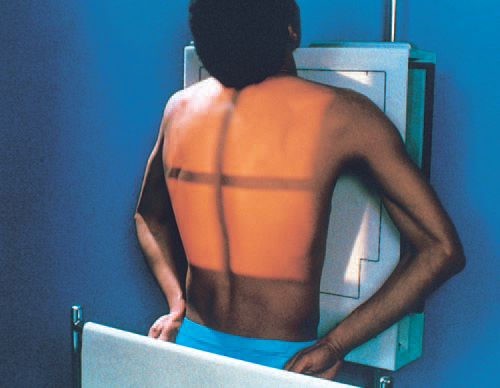
\includegraphics[width=0.7\linewidth]{imagenes/torax position}
		\caption{}
		\label{fig:torax-position}
	\end{figure}
	
	
	\paragraph{Rayo Central}
	Perpendicular al plano del receptor (0°). Punto de entrada: \textbf{T7}, usando el ángulo inferior de las escápulas como reparo anatómico.
	
	\paragraph{Receptor de imagen}
	Centrado en T7. Borde superior 4 a 5 cm por encima de los hombros para incluir los vértices. El plano medio sagital del paciente coincide con la línea media del receptor.
	
	\paragraph{Respiración}
	Inspiración forzada máxima, sostenida durante la exposición. Garantiza la máxima expansión del tórax en los tres ejes y el descenso del diafragma. En sospecha de neumotórax: dos exposiciones, una al final de inspiración forzada y otra al final de espiración forzada. La comparación evidencia aire libre pleural oculto en inspiración; también demuestra movilidad diafragmática, cuerpo extraño y atelectasia.
	
	\subsubsection*{4. Anatomía Visible}
	
	Tráquea aireada en línea media. Ambos campos pulmonares completos desde vértices hasta ángulos costofrénico y cardiofrénico. Cúpulas diafragmáticas. Silueta cardiaca y botón aórtico. Trama vascular pulmonar y árbol bronquial. Costillas, clavículas, escápulas proyectadas fuera de los campos y columna torácica. La trama pulmonar debe ser visible a través de la silueta cardiaca. Los ángulos costofrénico y cardiofrénico deben visualizarse íntegros.
	
	\subsubsection*{5. Criterios de Evaluación}
	
	\textbf{Posicionamiento correcto:} campos pulmonares íntegros incluyendo vértices y ángulos costofrénico y cardiofrénico; \textbf{9 a 10 arcos costales posteriores} (horizontales) y \textbf{6 a 7 arcos costales anteriores} (curvos) visibles por encima de las cúpulas; contornos definidos del corazón y el diafragma; marcas pulmonares desde el hilio a la periferia; marca de lado derecho en la imagen.
	
	\textbf{Ausencia de rotación:} extremidades mediales de ambas clavículas equidistantes de la columna (si la izquierda parece más corta, el paciente está rotado hacia la izquierda); apófisis espinosas centradas en la línea media; tráquea en la línea media.
	
	\textbf{Penetración y contraste:} trama pulmonar visible a través de la silueta cardiaca, confirmando la técnica ultra homogeneizada. Pulmones, mediastino y estructuras óseas diferenciados en la misma imagen.
	
	\subsubsection*{6. Puntos Críticos}
	
	\textbf{Rotación del paciente:} asimetría de clavículas y distorsión de la sombra cardiaca. Corrección: pedir que adelante el hombro más alejado del Bucky y lo presione hasta que ambos queden en contacto firme y parejo. Si una clavícula aparece más alta, indicarle que al inspirar no eleve los hombros y los relaje en un plano horizontal paralelo al piso.
	
	\textbf{Escápulas superpuestas a los campos:} ocurre cuando los brazos no están en jarra o los codos no se orientan hacia adelante. La rotación interna del húmero es la que desplaza las escápulas.
	
	\textbf{Inspiración insuficiente:} menos de 9 costillas posteriores visibles, campos condensados y corazón aparentemente agrandado. Indicador de inspiración correcta: 9--10 costillas posteriores y 6--7 anteriores, con trama pulmonar visible a través del corazón.
	
	\textbf{Corte de ángulos:} pérdida de información diagnóstica crítica; repetir siempre que sea posible.
	
	\textbf{Adaptaciones:} paciente que no puede estar de pie: AP en sedestación o decúbito, la mayor magnificación cardiaca es esperada y debe consignarse. Mamas voluminosas: elevarlas y separarlas. Clavícula congénitamente más alta: no confundir con rotación.
	
	\textbf{Trucos:} espesor medido a los 2/3 del tórax, no en el punto más grueso. La DFRI larga compensa la pérdida de mAs de las homogenizaciones. Si no se ve trama a través del corazón, el kVp o las homogenizaciones fueron insuficientes. La PA magnifica menos el corazón que la AP, relevante para medir el índice cardiotorácico.
	
	
	\clearpage
	
	\begin{figure*}[h]
		\centering
		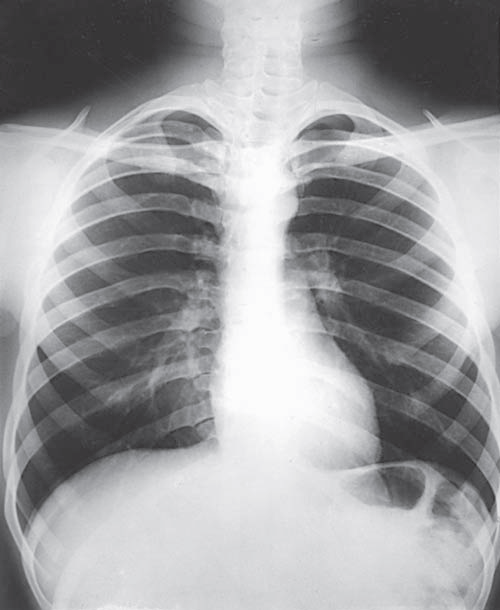
\includegraphics[width=0.7\linewidth]{imagenes/image}
		\caption[]{Torax PA}
		\label{fig:frentedetoraxPA}
	\end{figure*}
	
\clearpage
	%----------------------------------------------------------
	%  Para agregar otro enfoque duplicá el bloque
	%  desde \subsection hasta \textbf{Trucos}
	%----------------------------------------------------------


%%%%%%%%%%%%%%%%%%%%%%%%%%%%%%%%%%%%%%%%%%%%%%%%%%%%%%%%%%%
%  SECCIÓN: Tórax
%  Archivo: secciones/torax.tex
%  Sin preámbulo ni \begin{document} — lo maneja main.tex
	%%%%%%%%%%%%%%%%%%%%%%%%%%%%%%%%%%%%%%%%%%%%%%%%%%%%%%%%%%%
	
	\section{Tórax}
	
	\subsection{Proyección Lateral de Tórax (D o I)}
	
	\subsubsection*{1. Identificación}
	
	\textbf{Tipo:} Proyección básica. Forma par con la proyección posteroanterior (PA) de tórax.
	
	\textbf{Indicaciones clínicas principales:}
	\begin{itemize}
		\item Demostración de patologías situadas por detrás del corazón, grandes vasos y el esternón.
		\item Demostración de fisuras interlobulares y diferenciación de lóbulos pulmonares.
		\item Localización de lesiones pulmonares (complementa la proyección frontal).
		\item Hemotórax (presencia de sangre en cavidad pleural).
		\item Neumotórax (pérdida de trama pulmonar).
	\end{itemize}
	
	\subsubsection*{2. Técnica Base}
	
	\textbf{Receptor de imagen:} 35 × 43 cm. Orientación \textbf{longitudinal (vertical)}, con el borde superior ubicado 4 a 5 cm por encima de los hombros.
	
	\textbf{DFRI:} 180 a 200 cm. Distancia aumentada para minimizar la magnificación de las estructuras mediastínicas (reducir la divergencia del haz) y mejorar el detalle óseo de las estructuras torácicas. Contribuye además a la radioprotección del paciente.
	
	\textbf{Técnica:} Ultra homogeneizada (5 o 6 homogenizaciones). Permite obtener una escala de grises larga, reduciendo el contraste y posibilitando la visualización simultánea del parénquima pulmonar, el mediastino y las estructuras óseas, incluyendo la trama pulmonar detrás de las costillas y el corazón.
	
	\textbf{Factores técnicos:} kVp \textbf{igual al utilizado en la proyección frontal} --- mAs \textbf{= mAs del frente × 4} (factor 3,5 estándar; factor 4 en pacientes obesos). El factor de multiplicación compensa el mayor espesor que debe atravesar el rayo central en la proyección lateral.
	
	\textbf{Bucky:} Bucky mural con grilla. Obligatorio dado el espesor de la región y la técnica de alta tensión utilizada.
	
	\subsubsection*{3. Posicionamiento}
	
	\paragraph{Paciente}
	Paciente en bipedestación o sedestación. Plano medio sagital (PMS) paralelo al receptor de imagen. El peso corporal se distribuye de manera equitativa entre ambas piernas. La posición vertical favorece el descenso del diafragma por acción de la gravedad, permitiendo mejor visualización de los campos pulmonares y los ángulos costofrénicos, facilita la demostración de niveles hidroaéreos y evita la ingurgitación de los vasos sanguíneos pulmonares.
	
	\paragraph{Región de interés}
	Se coloca el hombro adyacente al receptor apoyado sobre el mismo. Se indica al paciente que levante los brazos por encima de la cabeza, agarrándose los codos entre sí o sosteniéndose de un soporte, para evitar que las partes blandas de los miembros superiores se superpongan a los campos pulmonares. En pacientes inestables se coloca un soporte auxiliar. Se indica elevar el mentón y mirar hacia adelante. El plano medio coronal se centra en la línea media del receptor para evitar rotaciones.
	
	\paragraph{Rayo Central}
	Perpendicular al plano del receptor. Punto de entrada: \textbf{plano medio coronal a la altura de T7 (equivalente al ángulo inferior de las escápulas)}.
	
	\paragraph{Receptor de imagen}
	Centrado a nivel de T7. Borde superior 4 a 5 cm por encima de los hombros, para incluir los vértices pulmonares. La región abarcada comprende desde las clavículas hasta los ángulos costofrénicos, incluyendo ambos campos pulmonares y el mediastino completo.
	
	\paragraph{Respiración}
	Exposición al final de una inspiración forzada (máxima). Garantiza la máxima expansión del tórax en los tres ejes, permitiendo correcta visualización de los campos pulmonares y los ángulos costofrénicos. Luego del disparo se indica al paciente que retome la respiración con normalidad.
	
	\begin{figure}[h]
		\centering
		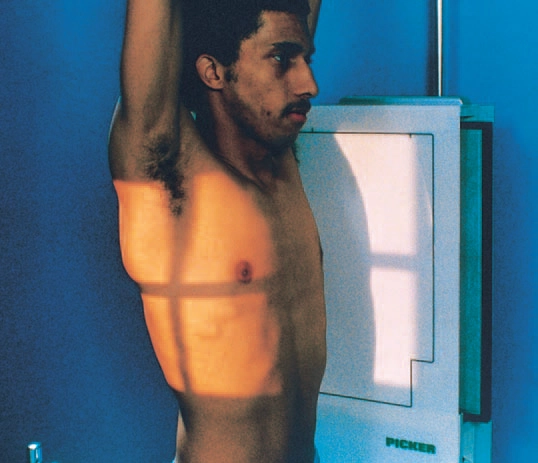
\includegraphics[width=0.7\linewidth]{imagenes/posicion torax perfil}
		\caption{}
		\label{fig:posicion-torax-perfil}
	\end{figure}
	
	
	
	
	
	\subsubsection*{4. Anatomía Visible}
	
	Corazón y aorta. Fisuras interlobulares (diferenciación de lóbulos pulmonares). Campos pulmonares en toda su extensión vertical. Mediastino anterior y posterior. Esternón de perfil. Cuerpos vertebrales torácicos con espacios intervertebrales y agujeros intervertebrales. Hilios pulmonares (ubicados aproximadamente en el centro de la radiografía). Ángulos costofrénicos. Hemidiafragmas. Arcos costales posteriores superpuestos a la columna vertebral.
	
	\subsubsection*{5. Criterios de Evaluación}
	
	\textbf{Posicionamiento correcto:} Esternón en posición de perfil verdadero. Eje largo de los campos pulmonares demostrado en posición vertical, sin inclinación anterior ni posterior. Ángulos costofrénicos y porción inferior de los vértices pulmonares incluidos. Brazos y partes blandas de los miembros superiores sin superponerse a la porción superior de los campos pulmonares. Hilios ubicados en el centro aproximado de la imagen.
	
	\textbf{Ausencia de rotación:} Arcos costales posteriores superpuestos a los cuerpos vertebrales. El lado alejado del receptor puede aparecer mínimamente por detrás del lado apoyado por efecto de la divergencia del haz (hallazgo normal esperado). Bordes posteriores de las vértebras visibles como una línea única. Espacios intervertebrales torácicos abiertos y agujeros intervertebrales visualizables (excepto en pacientes con escoliosis). Contornos nítidos del corazón y el diafragma.
	
	\textbf{Penetración y contraste:} Escala de grises larga que permita visualizar simultáneamente el parénquima pulmonar, el mediastino y las estructuras óseas. Penetración adecuada de los campos pulmonares y del corazón.
	
	\subsubsection*{6. Puntos Críticos}
	
	\textbf{Rotación del paciente:} Distorsiona la sombra cardíaca y compromete la evaluación del mediastino. Corrección: recolocar los hombros de modo que el PMS quede paralelo al receptor y el plano medio coronal perpendicular al mismo.
	
	\textbf{Brazos no elevados correctamente:} Las partes blandas de los miembros superiores se superponen a los vértices pulmonares, enmascarando patología. Corrección: indicar al paciente que lleve los brazos bien por encima de la cabeza, agarrándose los codos o sosteniéndose de un soporte.
	
	\textbf{Adaptaciones:} En pacientes con trauma o imposibilidad de bipedestación se realiza en sedestación o en decúbito lateral con rayo horizontal. En pacientes inestables se utiliza soporte auxiliar (gotero, barra) para mantener la posición de los brazos.
	
	\textbf{Trucos:} La proyección lateral izquierda es el estándar de referencia: el corazón queda más próximo al receptor, minimizando su magnificación y permitiendo mejor evaluación de la silueta cardíaca. Solo se realiza lateral derecha cuando está específicamente indicado (por ejemplo, para evaluar el pulmón derecho en detalle). El factor de multiplicación de mAs (×4) se aplica siempre respecto a los mAs de la proyección frontal, no de forma independiente.
	
	%----------------------------------------------------------
	%  Para agregar otro enfoque duplicá el bloque
	%  desde \subsection hasta \textbf{Trucos}
	%----------------------------------------------------------


\begin{figure*}[h]
	\centering
	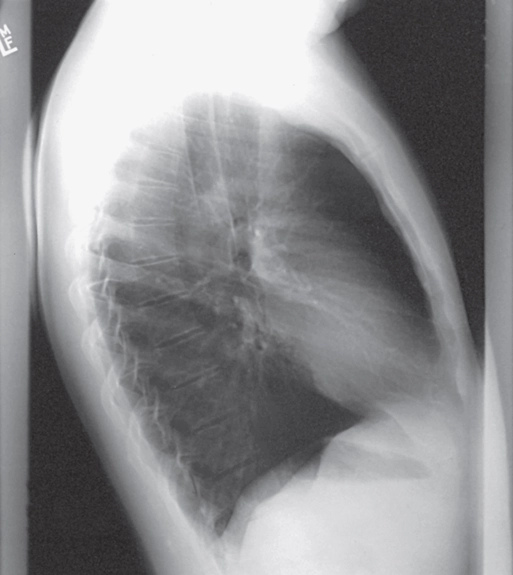
\includegraphics[width=0.7\linewidth]{imagenes/torax perfil rx}
	\caption{}
	\label{fig:torax-perfil-rx}
\end{figure*}




\clearpage
	
%%%%%%%%%%%%%%%%%%%%%%%%%%%%%%%%%%%%%%%%%%%%%%%%%%%%%%%%%%%
%  SECCIÓN: Tórax
%  Archivo: secciones/torax.tex
%  Sin preámbulo ni \begin{document} — lo maneja main.tex
	%%%%%%%%%%%%%%%%%%%%%%%%%%%%%%%%%%%%%%%%%%%%%%%%%%%%%%%%%%%
	
	\section{Tórax}
	
	\subsection{Tórax Portátil (Proyección AP)}
	
	\subsubsection*{1. Identificación}
	
	\textbf{Tipo:} Proyección de emergencia/adaptada. Sustituto de la proyección PA estándar cuando el paciente no puede ser trasladado.
	
	\textbf{Indicaciones clínicas principales:}
	\begin{itemize}
		\item Pacientes críticos o no colaborativos en UCI o sala de internación.
		\item Control de posición de dispositivos médicos (sondas, catéteres, tubo endotraqueal).
		\item Seguimiento de patología torácica en pacientes con imposibilidad de bipedestación.
		\item Sospecha de derrame pleural, neumotórax o consolidación en contexto de urgencia.
	\end{itemize}
	
	\subsubsection*{2. Técnica Base}
	
	\textbf{Receptor de imagen:} 35 × 43 cm. Orientación \textbf{transversal} en pacientes hiperesténicos y esténicos; \textbf{longitudinal} en pacientes asténicos e hipoesténicos, para incluir correctamente el eje longitudinal del tórax según el hábito corporal. Borde superior 4 a 5 cm por encima de los hombros.
	
	\textbf{DFRI:} La mayor distancia que permita el equipo y la situación clínica. \textbf{Mínima de 100 cm.} A menor distancia se incrementa la magnificación del mediastino; con la distancia habitual de trabajo portátil se genera una magnificación aproximada del 15\% respecto a la proyección PA estándar.
	
	\textbf{Técnica:} Ajustada a la distancia real de trabajo y a la ausencia de Bucky. Se reduce el kVp respecto a la técnica estándar para disminuir la radiación secundaria por efecto Compton, compensando la falta de grilla y mejorando el contraste de la imagen.
	
	\textbf{Factores técnicos:} kVp \textbf{reducido respecto a la técnica estándar} --- mAs \textbf{ajustado a la distancia utilizada}. Sin método de medición de espesor estandarizado; se ajusta según las condiciones del paciente y el equipo disponible.
	
	\textbf{Bucky:} No disponible. La ausencia de Bucky y de grilla es una limitación inherente a la técnica portátil; genera mayor ruido y menor contraste respecto a la técnica estándar.
	
	\subsubsection*{3. Posicionamiento}
	
	\paragraph{Paciente}
	Paciente lo más erguido posible, idealmente a 90° en la camilla (sedestación o semisentado). La posición vertical favorece la detección de derrames pleurales, neumotórax y niveles hidroaéreos. En posición supina o con escasa elevación estas patologías son más difíciles de detectar por pérdida del efecto gravitacional.

	\paragraph{Región de interés}
	Se indica rodar los hombros del paciente hacia adelante, rotando los brazos medial o internamente, para alejar las escápulas de los campos pulmonares. Se centra al paciente respecto al rayo central y al receptor, verificando la alineación visionando al paciente desde la parte superior, cerca del tubo.


	\paragraph{Rayo Central}
	Perpendicular al receptor y al esternón. Si es necesario, se angula caudalmente (aproximadamente ±5°) hasta lograr la perpendicularidad respecto al eje longitudinal del esternón, para impedir que las clavículas oculten los vértices pulmonares. Punto de entrada: \textbf{T7, aproximadamente 8 a 10 cm por debajo de la escotadura yugular}.
	
	\paragraph{Receptor de imagen}
	Colocado detrás del tórax del paciente, centrado a nivel de T7. Borde superior 4 a 5 cm por encima de los hombros. Orientación adaptada al hábito corporal del paciente (ver sección Técnica Base).
	
	\paragraph{Respiración}
	Idealmente suspendida al final de una inspiración completa. Dado que muchos pacientes no pueden colaborar plenamente, se recomienda visualizar el tórax del paciente y disparar en el momento de mayor volumen respiratorio visible.
	
	
	\begin{figure}[h]
		\centering
		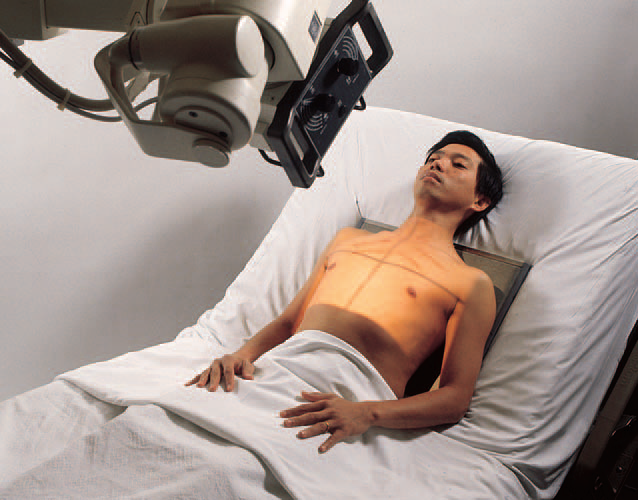
\includegraphics[width=0.7\linewidth]{imagenes/torax portatil}
		\caption{}
		\label{fig:torax-portatil}
	\end{figure}
	
	
	\subsubsection*{4. Anatomía Visible}
	
	Campos pulmonares. Silueta cardíaca (con magnificación inherente a la técnica). Mediastino. Estructuras óseas torácicas (costillas, clavículas, esternón proyectado). Hemidiafragmas y ángulos costofrénicos (con limitaciones en posición supina). Dispositivos médicos en caso de estar presentes.
	
	\subsubsection*{5. Criterios de Evaluación}
	
	\textbf{Posicionamiento correcto:} Escápulas alejadas de los campos pulmonares. Tórax centrado respecto al receptor. Inclusión de ambos ángulos costofrénicos y vértices pulmonares. Borde superior del receptor 4 a 5 cm por encima de los hombros.
	
	\textbf{Ausencia de rotación:} Simetría de las articulaciones esternoclaviculares respecto a la columna vertebral. Columna vertebral centrada en la imagen.
	
	\textbf{Penetración y contraste:} Se deben mantener los mismos criterios de valor diagnóstico que en la radiografía estándar. Se aceptan tres variaciones inherentes a la técnica: (1) silueta cardíaca magnificada por el menor DFRI y el aumento de la distancia objeto-receptor; (2) posible ocultamiento de la trama vascular por derrame pleural; (3) visualización de solo 8 a 9 costillas posteriores por inspiración incompleta, con pulmones de mayor densidad aparente al no estar completamente ventilados.
	
	\subsubsection*{6. Puntos Críticos}
	
	\textbf{Magnificación del mediastino:} Consecuencia directa del menor DFRI y de la proyección AP. No es un error técnico sino una limitación estructural de la técnica; debe tenerse en cuenta al evaluar el índice cardiotorácico.
	
	\textbf{Ausencia de Bucky:} Genera mayor ruido y menor contraste. Se compensa reduciendo el kVp para disminuir la radiación secundaria por efecto Compton.
	
	\textbf{Adaptaciones:} En pacientes en decúbito supino estricto se realiza la proyección en esa posición, asumiendo las limitaciones diagnósticas para derrame pleural, neumotórax y niveles hidroaéreos. En pacientes con múltiples dispositivos médicos se solicita ayuda al personal del área para posicionar el receptor sin traccionar ni desconectar los dispositivos.
	
	\textbf{Trucos:} La calidad de imagen de una radiografía portátil nunca debe aceptarse como inferior por el solo hecho de serlo; el objetivo sigue siendo alcanzar los mismos criterios diagnósticos de la proyección estándar dentro de las limitaciones del contexto. Visualizar al paciente desde arriba (cerca del tubo) antes de disparar permite verificar la alineación sin movilizarlo.
	
	
	\begin{figure*}[h]
		\centering
		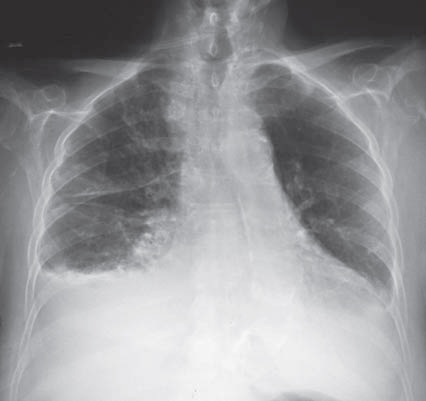
\includegraphics[width=0.7\linewidth]{imagenes/torax portatil 2}
		\caption{}
		\label{fig:torax-portatil-2}
	\end{figure*}
	
	\clearpage
	
	%----------------------------------------------------------
	%  Para agregar otro enfoque duplicá el bloque
	%  desde \subsection hasta \textbf{Trucos}
	%----------------------------------------------------------
	
	
	%%%%%%%%%%%%%%%%%%%%%%%%%%%%%%%%%%%%%%%%%%%%%%%%%%%%%%%%%%%
	%  SECCIÓN: Tórax
	%  Archivo: secciones/torax.tex
	%  Sin preámbulo ni \begin{document} — lo maneja main.tex
		%%%%%%%%%%%%%%%%%%%%%%%%%%%%%%%%%%%%%%%%%%%%%%%%%%%%%%%%%%%
		
		\section{Tórax}
		
		\subsection{Vértices Pulmonares (Método de Lindblom / Posición Lordótica)}
		
		\subsubsection*{1. Identificación}
		
		\textbf{Tipo:} Proyección complementaria. Debe realizarse luego de la proyección PA y perfil de tórax convencionales.
		
		\textbf{Indicaciones clínicas principales:}
		\begin{itemize}
			\item Tuberculosis pulmonar (bacilo de Koch) y sospecha de focos apicales
			\item Nódulos, masas o tumores en vértices pulmonares
			\item Casquetes apicales y calcificaciones en región de los vértices
			\item Descartar patología pulmonar superior no visible en PA convencional por superposición clavicular
		\end{itemize}
		
		\subsubsection*{2. Técnica Base}
		
		\textbf{Receptor de imagen:} 35 × 43 cm. Orientación \textbf{longitudinal}. Borde superior del chasis ubicado 7--8 cm por encima de los hombros.
		
		\textbf{DFRI:} 180 cm. Igual que en tórax convencional, para reducir la magnificación del corazón y estructuras mediastínicas.
		
		\textbf{Técnica:} Ultra homogeneizada, igual que en tórax PA. Debe ser \textbf{ligeramente mayor} que en la PA convencional, dado el mayor espesor del tórax en posición oblicuada, que requiere mayor penetración para visualizar tejido pulmonar retroóseo.
		
		\textbf{Factores técnicos:} kVp \textbf{similar a tórax PA, levemente aumentado} --- mAs \textbf{levemente aumentado respecto a PA}. Espesor medido con el tórax en posición lordótica.
		
		\textbf{Bucky:} Bucky de pared con grilla, dado el espesor de la región.
		
		\subsubsection*{3. Posicionamiento}
		
		\paragraph{Paciente}
		Bipedestación a unos 30 cm del receptor. Plano medio sagital perpendicular al receptor. Posición AP: el paciente se inclina lentamente hacia atrás, apoyando hombros, cuello y nuca contra el Bucky de pared, manteniendo los pies fijos en el piso.
		
		\paragraph{Región de interés}
		Ambas manos sobre las caderas con las palmas hacia afuera y los hombros proyectados hacia adelante. El dorso de las escápulas queda en contacto con el receptor. La hiperextensión del tórax proyecta las clavículas hacia arriba, liberando los vértices pulmonares de su superposición.
		
		\paragraph{Rayo Central}
		\textbf{Opción preferida (paciente apto):} Perpendicular al plano del receptor. Punto de entrada: \textbf{zona media del esternón}.\\
		\textbf{Opción alternativa (paciente no logra lordosis):} Angulado \textbf{15--20° en sentido cefálico}, centrado en el \textbf{manubrio esternal}. Regla general: \textbf{siempre evitar angular cuando sea posible}.
		
		\paragraph{Receptor de imagen}
		Centrado en los vértices pulmonares. Borde superior 7--8 cm por encima de los hombros. Colimar \textbf{exclusivamente a los vértices pulmonares}, sin necesidad de incluir la totalidad de los campos pulmonares.
		
		\paragraph{Respiración}
		Inspiración máxima. Expande los pulmones y maximiza la visualización del tejido pulmonar apical.
		
		\begin{figure}[h]
			\centering
			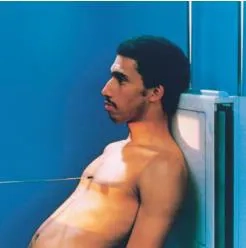
\includegraphics[width=0.7\linewidth]{imagenes/torax vertices}
			\caption{}
			\label{fig:torax-vertices}
		\end{figure}
		
		
		\begin{figure}[h]
			\centering
			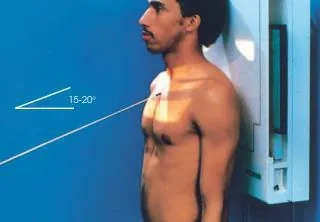
\includegraphics[width=0.7\linewidth]{imagenes/torax vertices 2}
			\caption[]{Variante}
			\label{fig:torax-vertices-2}
		\end{figure}
		
		
		\subsubsection*{4. Anatomía Visible}
		
		Vértices pulmonares bilaterales libres de superposición clavicular. Clavículas proyectadas por encima de los vértices en disposición horizontal. Primeras y segundas costillas con sus extremos mediales superpuestos a los extremos mediales de las clavículas. Segmentos anterior y posterior de las costillas superpuestos y distorsionados por la oblicuación del tórax. Región apical del parénquima pulmonar despejada para evaluar nódulos, infiltrados o calcificaciones.
		
		\subsubsection*{5. Criterios de Evaluación}
		
		\textbf{Posicionamiento correcto:} Clavículas situadas por encima de los vértices pulmonares, sin superponerse sobre el tejido pulmonar apical.
		
		\textbf{Ausencia de rotación:} Extremos mediales de ambas clavículas equidistantes respecto a la columna vertebral. Clavículas en disposición horizontal y simétrica.
		
		\textbf{Penetración y contraste:} Técnica ultra homogeneizada que permita visualizar el tejido pulmonar a través de la densidad ósea superpuesta. Los segmentos anteriores y posteriores de las costillas deben verse distorsionados y superpuestos, confirmando la correcta posición lordótica.
		
		\subsubsection*{6. Puntos Críticos}
		
		\textbf{Paciente no logra la posición lordótica:} Las clavículas permanecen superpuestas a los vértices. Corrección: angular el RC 15--20° en sentido cefálico, centrando en el manubrio. Introduce distorsión geométrica de la región.
		
		\textbf{Colimación excesiva:} Incluir la totalidad de los campos pulmonares implica irradiación innecesaria. Al ser proyección complementaria, la colimación debe restringirse a los vértices.
		
		\textbf{Adaptaciones:} En pacientes con dolor torácico agudo o limitación de movilidad, optar directamente por la angulación del RC (15--20° cefálico) sin forzar la posición lordótica.
		
		\textbf{Trucos:} Regla práctica de angulación: en AP (paciente frente al tubo) → ángulo craneal para elevar las clavículas; en PA → ángulo caudal para el mismo efecto. La técnica debe aumentarse respecto a la PA convencional por el mayor espesor efectivo del tórax oblicuado.
		
		
		
		\begin{figure*}[h]
			\centering
			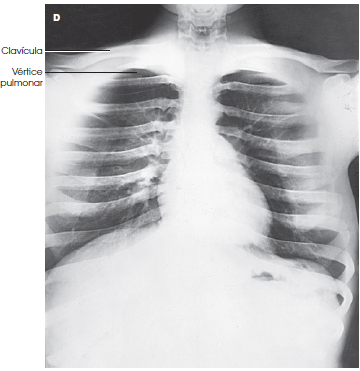
\includegraphics[width=0.7\linewidth]{imagenes/torax vertice 3}
			\caption{}
			\label{fig:torax-vertice-3}
		\end{figure*}
		
		\clearpage
		
		
		%----------------------------------------------------------
		%  Para agregar otro enfoque duplicá el bloque
		%  desde \subsection hasta \textbf{Trucos}
		%----------------------------------------------------------
	
	%%%%%%%%%%%%%%%%%%%%%%%%%%%%%%%%%%%%%%%%%%%%%%%%%%%%%%%%%%%
	%  SECCIÓN: Tórax
	%  Archivo: secciones/torax.tex
	%  Sin preámbulo ni \begin{document} — lo maneja main.tex
		%%%%%%%%%%%%%%%%%%%%%%%%%%%%%%%%%%%%%%%%%%%%%%%%%%%%%%%%%%%
		
		\section{Tórax}
		
		\subsection{Oblicuas Anteriores de Corazón y Grandes Vasos (OAD / OAI)}
		
		\subsubsection*{1. Identificación}
		
		\textbf{Tipo:} Proyecciones complementarias. Forman par entre sí: la OAD y la OAI se
		solicitan conjuntamente según la indicación clínica. \textbf{Solo se realizan oblicuas
			anteriores} para corazón y grandes vasos; las oblicuas posteriores están contraindicadas
		(mayor magnificación y exposición frontal del paciente al haz primario).
		
		\textbf{Nomenclatura:} Se nombran según el lado del cuerpo que se apoya contra el RI.
		
		  \begin{tcolorbox}[colback=red!5!white, colframe=red!80!black, fonttitle=\bfseries, title=Importante]
			\begin{itemize}
				\item \textbf{OAD} (Oblicua Anterior Derecha): hombro anterior \textbf{derecho} apoyado en el RI.
				\item \textbf{OAI} (Oblicua Anterior Izquierda): hombro anterior \textbf{izquierdo} apoyado en el RI.
			\end{itemize}
		\end{tcolorbox}
		
		\textbf{Principio de visualización:} El lado de interés diagnóstico es el más \textbf{alejado}
		del RI. Para ver la hemitórax izquierda (cayado aórtico, campo pulmonar izquierdo) → OAI;
		para ver la hemitórax derecha → OAD.
		
		\textbf{Indicaciones clínicas principales:}
		\begin{itemize}
			\item Bloque quirúrgico: control de stent, malla endovascular o aorta con contraste.
			\item Esofagograma y estudio gastroduodenal con contraste baritado (desplegar el esófago retrocardiaco).
			\item Valoración del cayado aórtico y aorta descendente (preferentemente OAI).
			\item Estudio del mediastino: separar la columna vertebral de las estructuras mediastínicas
			superpuestas en el frente PA estándar.
			\item Evaluación del campo pulmonar completo libre de superposición cardiaca o columnar.
		\end{itemize}
		
		\subsubsection*{2. Técnica Base}
		
		\textbf{Receptor de imagen:} 35 × 43 cm. Orientación \textbf{longitudinal} en todo tipo de paciente,
		para incluir ambos pulmones desde los vértices hasta los ángulos costofrénicos.
		
		\textbf{DFRI:} \textbf{180 cm}. La distancia foco-receptor incrementada reduce la magnificación
		de las estructuras mediastínicas, que en proyección PA quedan alejadas del RI, mejorando la
		nitidez geométrica y la fidelidad de tamaño.
		
		\textbf{Técnica:} Ultra-homogeneizada con \textbf{alto kVp} (escala larga de grises). Permite
		visualizar simultáneamente el parénquima pulmonar y el mediastino, que de otro modo quedarían
		enmascarados por la superposición ósea y la densidad cardiaca. Variantes según paciente:
		\begin{itemize}
			\item \textit{Paciente obeso:} técnica intermedia; mayor radiación dispersa, puede requerirse
			incremento controlado de mAs.
			\item \textit{Control de stent o malla metálica:} kVp muy alto para ``atravesar'' la densidad
			cardiaca y revelar el metal con claridad, priorizando transparencia.
		\end{itemize}
		
		\textbf{Factores técnicos:} kVp \textbf{alto} --- mAs según hábito corporal.
		Espesor medido a nivel del tórax en su diámetro AP.
		
		\textbf{Bucky:} Sí. Bucky mural (vertical) con grilla, dado el espesor del tórax y la
		producción significativa de radiación dispersa.
		
		\subsubsection*{3. Posicionamiento}
		
		\paragraph{Paciente}
		Bipedestación (de pie) o, si no es posible, sedestación erguida. Posición PA: el tórax
		enfrenta el RI y la espalda queda dirigida hacia el tubo, lo que protege las estructuras
		radiosensibles anteriores (radioprotección activa). El mentón elevado, mirando hacia adelante,
		sin rotar la cabeza.
		
		\begin{figure}[h]
			\centering
			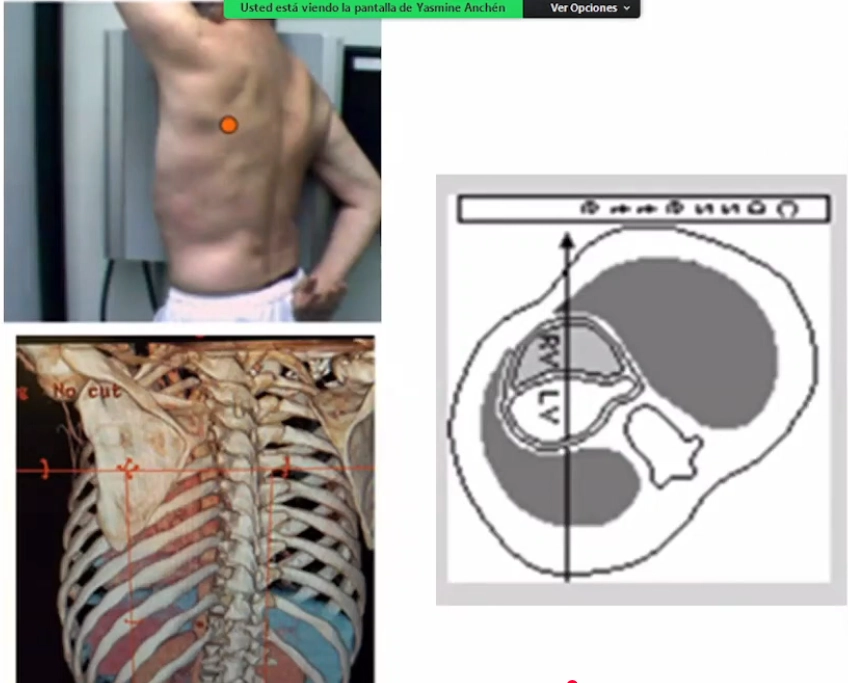
\includegraphics[width=0.7\linewidth]{imagenes/grandes vasos OAD}
			\caption[]{OAD grandes vasos}
			\label{fig:grandes-vasos-oad}
		\end{figure}
		
		\begin{figure}[h]
			\centering
			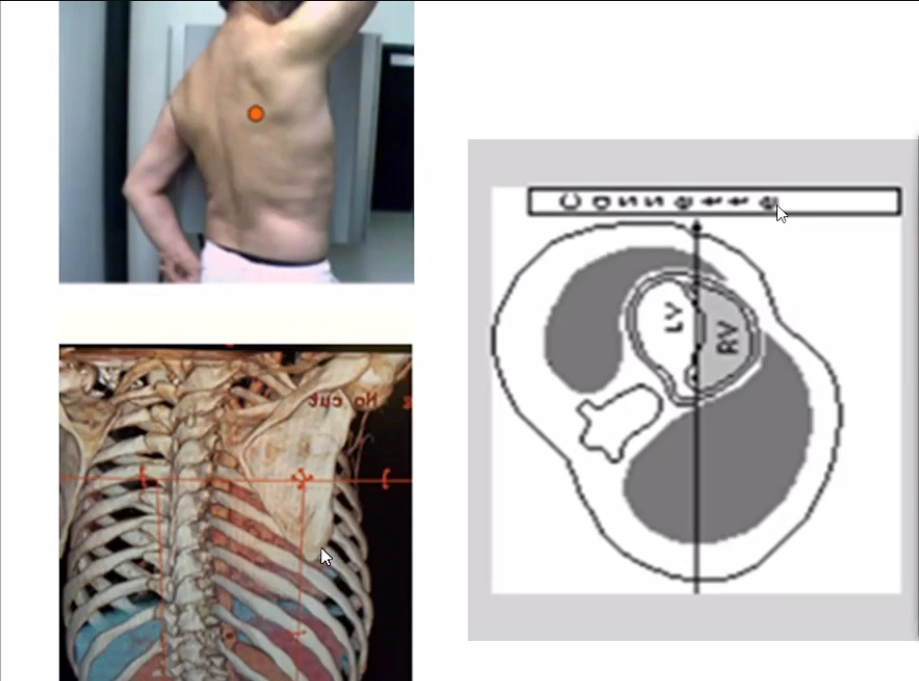
\includegraphics[width=0.7\linewidth]{imagenes/grandes vasos OAI}
			\caption[]{OAI grandes vasos}
			\label{fig:grandes-vasos-oai}
		\end{figure}
		
		
		\paragraph{Región de interés}
		Rotación del tórax sobre su eje longitudinal alejando el lado de interés del RI:
		\textbf{45°} para estudio del \textbf{pulmón} y \textbf{60°} para estudio del
		\textbf{corazón y grandes vasos}, medidos desde el plano frontal.
		\begin{itemize}
			\item \textit{OAD:} se aleja el hombro izquierdo; el hombro anterior derecho queda apoyado en el RI.
			\item \textit{OAI:} se aleja el hombro derecho; el hombro anterior izquierdo queda apoyado en el RI.
		\end{itemize}
		Posición de los miembros superiores: del \textit{lado apoyado}, la mano se coloca sobre la
		cadera con la palma hacia afuera; del \textit{lado alejado}, el paciente eleva el brazo hasta
		la altura del hombro y apoya la mano sobre la cabeza para no tapar el campo pulmonar.
		Variante: ambos codos tomados por encima de la cabeza. Los hombros deben quedar en un mismo
		plano horizontal.
		
		\paragraph{Rayo Central}
		Perpendicular al plano del RI, sin angulación. Punto de entrada:
		\begin{itemize}
			\item \textbf{OAD:} ángulo inferior de la escápula \textbf{izquierda} (lado alejado).
			\item \textbf{OAI:} ángulo inferior de la escápula \textbf{derecha} (lado alejado).
		\end{itemize}
		Referencia alternativa equivalente: \textbf{T7}, aproximadamente 8--10 cm por debajo de la
		escotadura yugular (referenciando C7).
		
		\paragraph{Receptor de imagen}
		Centrado respecto al eje del tórax del paciente. Borde superior situado
		\textbf{4--5 cm por encima de C7} (vértebra prominente). Debe incluir ambos pulmones completos:
		desde los vértices pulmonares hasta los ángulos costofrénicos inferiores, y la totalidad de
		las estructuras mediastínicas (tráquea, cayado aórtico, silueta cardiaca).
		
		\paragraph{Respiración}
		\textbf{Inspiración máxima sostenida} (``Respire todo lo que pueda y aguante el aire'').
		Desciende el diafragma, expande los campos pulmonares y aumenta el contraste aire/tejido blando,
		mejorando la visualización del parénquima y las estructuras vasculares. Control: deben contarse
		\textbf{9--10 arcos costales posteriores} por encima de la cúpula diafragmática (los arcos
		posteriores son más horizontales y más fáciles de identificar). Si solo se observan 8,
		la inspiración fue insuficiente y debe repetirse.
		
		\subsubsection*{4. Anatomía Visible}
		
		\textbf{En OAD:} silueta cardiaca de morfología \textbf{triangular}; espacio aéreo
		retroesternal anterior con forma triangular; cayado aórtico \textit{sin desplegar}
		(superpuesto); tráquea llena de aire y árbol bronquial \textbf{izquierdo} completamente
		desplegado; cámara gástrica \textbf{alejada} de la columna (``posición de esgrimista'');
		campo pulmonar izquierdo en mayor extensión.
		
		\textbf{En OAI:} silueta cardiaca de morfología \textbf{en pera} (ventrículo izquierdo
		proyectado hacia la izquierda inferior); \textbf{cayado aórtico desplegado} con aorta
		ascendente, cayado y aorta descendente separados y nítidos; espacio aéreo anterior de
		morfología \textbf{rectangular}; cámara gástrica \textbf{próxima} a la columna
		(``posición de boxeador''); campo pulmonar derecho en mayor extensión; esófago retrocardiaco
		visible cuando se usa contraste baritado.
		
		En ambas proyecciones: bifurcación traqueal (carina) proyectada \textbf{sobre la silueta
			cardiaca}, nunca sobre la columna vertebral.
		
		\subsubsection*{5. Criterios de Evaluación}
		
		\textbf{Posicionamiento correcto:} OAD → corazón triangular, espacio aéreo anterior
		triangular, cámara gástrica alejada de la columna, árbol bronquial izquierdo desplegado.
		OAI → corazón en pera, cayado aórtico desplegado, espacio aéreo anterior rectangular,
		cámara gástrica próxima a la columna. En ambas: carina sobre la silueta cardiaca y hombros
		en el mismo plano horizontal.
		
		\textbf{Ausencia de rotación:} la columna vertebral no debe superponerse al campo pulmonar
		contralateral (exceso de rotación); el corazón no debe quedar encimado a la columna (falta
		de rotación). La tráquea debe mostrar un perfil aéreo nítido y continuo.
		
		\textbf{Penetración y contraste:} escala larga de grises que permita visualizar
		simultáneamente el parénquima pulmonar y el mediastino. La trama vascular debe ser visible
		hasta la periferia. El corazón no debe ser completamente radiopaco: deben poder evaluarse
		las estructuras retrocardiacas. 9--10 arcos costales posteriores visibles sobre el diafragma
		confirman inspiración adecuada.
		
		\subsubsection*{6. Puntos Críticos}
		
		\textbf{Corazón encimado a la columna (OAI):} falta de rotación; el mediastino no se despliega.
		Corrección: aumentar la rotación hasta 60° y verificar posición de hombros.
		
		\textbf{Columna tapando el campo pulmonar contralateral:} rotación excesiva (demasiado de
		perfil). Corrección: reducir el grado de rotación.
		
		\textbf{Corazón muy radiopaco sin poder atravesarlo:} kVp insuficiente. Corrección: subir kVp
		para obtener escala larga de grises.
		
		\textbf{Imagen con apariencia de parrilla costal:} técnica ósea aplicada erróneamente;
		no se ve la trama pulmonar. Corrección: técnica ultra-homogeneizada con alto kVp.
		
		\textbf{Adaptaciones:} en pacientes con limitación para la bipedestación, realizar en
		sedestación erguida. En bloque quirúrgico (control de stent o malla), priorizar alto kVp
		con escala muy larga para revelar el material metálico a través de la densidad cardiaca.
		
		\textbf{Trucos:}
		\begin{itemize}
			\item Para desplegar el cayado aórtico: siempre OAI. En OAD el cayado queda superpuesto
			y no es valorable.
			\item Nemotecnia: \textit{esgrimista} = OAD (cámara gástrica alejada de la columna);
			\textit{boxeador} = OAI (cámara gástrica próxima a la columna).
			\item Contar arcos \textbf{posteriores} para evaluar la inspiración, no los anteriores;
			son más horizontales y más fáciles de identificar.
			\item Si en un examen preguntan si se realiza oblicua \textit{posterior} para corazón
			→ \textbf{FALSO}: solo se realizan oblicuas anteriores.
		\end{itemize}
		
		\begin{figure*}[t]
			\centering
			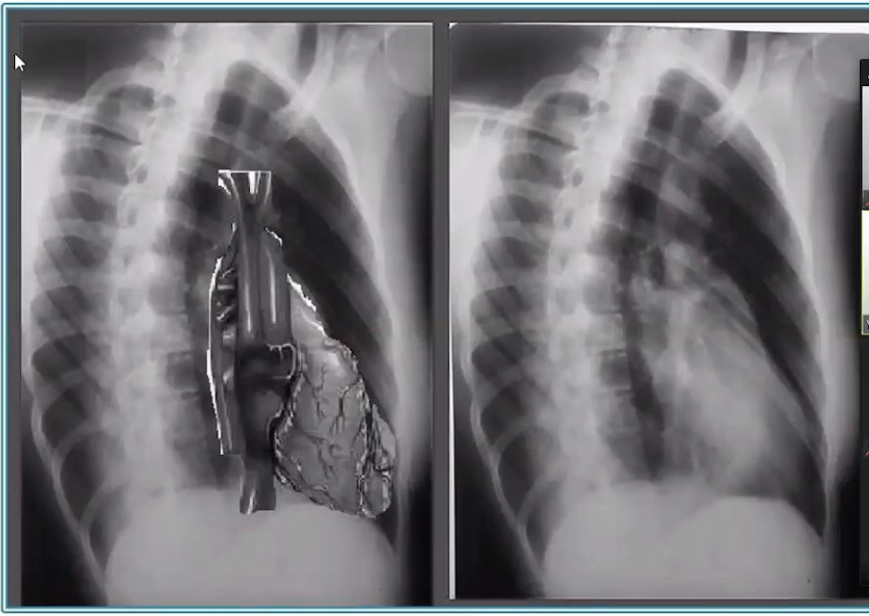
\includegraphics[width=0.7\linewidth]{imagenes/grandes vasos RX OAD}
			\caption[]{OAD de grandes vasos}
			\label{fig:grandes-vasos-rx-oad}
		\end{figure*}
		
	\clearpage
	
		\begin{figure*}[t]
			\centering
			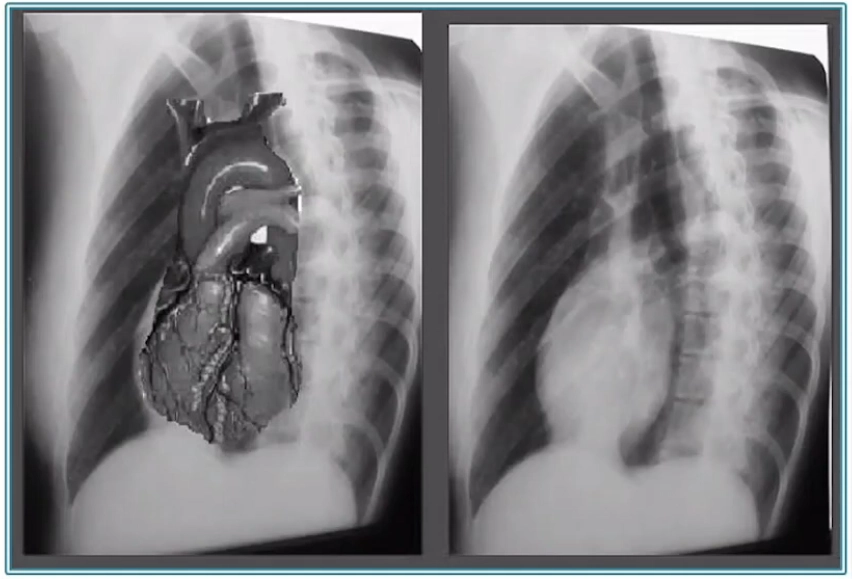
\includegraphics[width=0.7\linewidth]{imagenes/grandes vasos RX OAI}
			\caption[]{OAI de grandes vasos}
			\label{fig:grandes-vasos-rx-oai}
		\end{figure*}
		
\clearpage
		
		%----------------------------------------------------------
		%  Para agregar otro enfoque duplicá el bloque
		%  desde \subsection hasta \textbf{Trucos}
		%----------------------------------------------------------
		
		

	
	%%=========================================================
	%%  ENFOQUE 1: Parrilla Costal — Frente (Supra diafragmática)
	%%=========================================================
	\section{Tórax}
	\subsection{Parrilla Costal Frente Supra Diafragmática}
	
	\subsubsection*{1. Identificación}
	
	\textbf{Tipo:} Proyección básica. Primer estudio de la parrilla costal supra diafragmática; forma par con la proyección oblicua costal correspondiente.
	
	\textbf{Indicaciones clínicas principales:}
	\begin{itemize}
		\item Traumatismo de parrilla costal con sospecha de fractura de arcos costales superiores (1.º--10.º)
		\item Dolor costal agudo o crónico de localización superior al diafragma
		\item Evaluación post-protocolo de tórax PA para descartar neumotórax o hemotórax
	\end{itemize}
	
	\textbf{Nota de anamnesis:} Antes de iniciar el estudio verificar: (1) naturaleza y mecanismo del traumatismo; (2) localización exacta del dolor; (3) presencia de dificultad respiratoria; (4) capacidad del paciente para la bipedestación.
	
	\subsubsection*{2. Técnica Base}
	
	\textbf{Receptor de imagen:} 35 $\times$ 43 cm. Orientación \textbf{longitudinal}.
	
	\textbf{DFRI:} 100 cm. Distancia estándar de tórax; reduce la ampliación geométrica y permite incluir la totalidad de la caja torácica superior.
	
	\textbf{Técnica:} \textbf{Homogeneizada o intermedia} (de preferencia según biotipo del paciente). Las costillas supra diafragmáticas están rodeadas de parénquima pulmonar aireado, por lo que no se requiere técnica básica de alta diferenciación de partes blandas.
	
	\textbf{Factores técnicos:} kVp \textbf{65--70}. Un kVp relativamente bajo mantiene el contraste radiológico y permite visualizar las costillas a través del pulmón lleno de aire. Si la lesión se proyecta sobre la silueta cardíaca, incrementar el kVp para obtener mayor penetración en esa región.
	
	\textbf{Bucky:} Bucky mural con grilla.
	
	\subsubsection*{3. Posicionamiento}
	
	\paragraph{Paciente}
	Bipedestación. La posición de pie favorece el descenso gravitacional del diafragma a su posición más baja, ampliando el campo pulmonar y facilitando una inspiración profunda. La orientación del estudio depende de la región a evaluar:
	\begin{itemize}
		\item \textbf{Arcos posteriores}: posición AP (dorso apoyado contra el receptor).
		
		\item \textbf{Arcos anteriores}: posición PA (tórax apoyado contra el receptor; los arcos anteriores quedan más próximos al receptor mejorando el detalle).
	\end{itemize}
	
	\paragraph{Región de interés}
	Plano medio sagital perpendicular al receptor e isocentrado. Se apoya siempre la región que se desea radiografiar para reducir la distancia objeto-receptor y minimizar la ampliación.
	

	
\paragraph{Rayo Central}
Perpendicular al plano del receptor.

\textbf{Bilateral:} centrado en \textbf{T7} (equivalente a la mitad del esternón).

\textbf{Unilateral:} centrado en la \textbf{línea medio clavicular} del hemitórax de interés, a la misma altura.
	
	\paragraph{Receptor de imagen}
	Centrado en T7 para estudios bilaterales, o en la línea medio clavicular ipsilateral para estudios unilaterales. El borde superior del receptor debe superar los ápices pulmonares y el borde inferior incluir hasta por debajo del diafragma.
	
	\paragraph{Respiración}
	\textbf{Inspiración profunda y apnea.} El descenso del diafragma expande los campos pulmonares y proyecta el diafragma por debajo de la 9.ª--10.ª costilla posterior, evitando la superposición sobre los arcos costales superiores. En pacientes con dolor intenso la inspiración puede ser limitada, por lo que en ocasiones solo se visualizan 8--9 costillas posteriores por encima del diafragma.
	
	\subsubsection*{4. Anatomía Visible}
	
	\textbf{Arcos costales posteriores del 1.º al 10.º} por encima del diafragma, proyectados a través del parénquima pulmonar. En la proyección PA se obtiene mejor detalle de los arcos anteriores por su proximidad al receptor. Los arcos costales anteriores presentan una imagen "cortada" en su porción cartilaginosa, ya que el cartílago no calcificado es radiotransparente. La mayor concentración de fracturas se localiza en el \textbf{borde axilar} de los arcos, zona que puede requerir proyecciones oblicuas adicionales para su correcta evaluación.
	
	\subsubsection*{5. Criterios de Evaluación}
	
	\textbf{Posicionamiento correcto:} Visualización de los arcos costales posteriores del 1.º al 10.º por encima del diafragma. En estudios unilaterales, las costillas contralaterales pueden estar incompletas sin pérdida diagnóstica.
	
	\textbf{Ausencia de rotación:} Simetría bilateral de las estructuras torácicas; distancias claviculares equidistantes respecto a la columna vertebral.
	
	\textbf{Penetración y contraste:} Visualización nítida de los arcos costales a través del parénquima pulmonar con contraste adecuado entre hueso y tejido pulmonar aireado.
	
	\subsubsection*{6. Puntos Críticos}
	
	\textbf{Técnica incorrecta (kVp excesivo):} Sobreexposición con pérdida de contraste óseo; los arcos costales se pierden en el fondo del parénquima. Utilizar kVp 65--70 como valor de referencia.
	
	\textbf{Fase respiratoria incorrecta (espiración):} El diafragma asciende y superpone sobre los arcos costales inferiores, reduciendo el número de costillas visibles. Instruir correctamente al paciente para inspiración profunda y apnea.
	
	\textbf{Adaptaciones:} En pacientes con dolor intenso que impide la bipedestación, realizar en decúbito supino (AP acostado); tener en cuenta que el diafragma asciende y puede superponerse sobre los arcos inferiores. Si el dolor impide una inspiración profunda, documentar la limitación y aceptar la imagen con 8--9 costillas visibles.
	
	\textbf{Trucos:} Recordar el \textbf{protocolo obligatorio de dos pasos}: primero radiografía de tórax PA para descartar neumotórax o hemotórax, luego el estudio específico de costillas. La localización del dolor determina si se realiza estudio supra o infra diafragmático.
	
		\begin{figure*}[t]
		\centering
		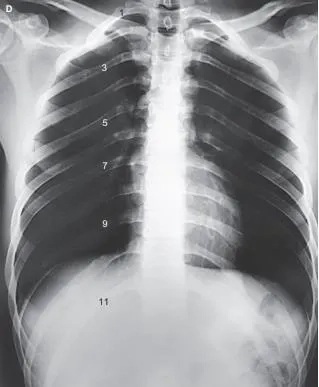
\includegraphics[width=0.7\linewidth]{imagenes/costilla supra}
		\caption{Arcos costales supra diafragmaticos}
		\label{fig:costilla-supra}
	\end{figure*}
	
\clearpage
	
	%----------------------------------------------------------
	
	%%=========================================================
	%%  ENFOQUE 2: Parrilla Costal — Frente (Infra diafragmática)
	%%=========================================================
	
	\subsection{Parrilla Costal Frente Infra Diafragmática}
	
	\subsubsection*{1. Identificación}
	
	\textbf{Tipo:} Proyección básica. Primer estudio de la parrilla costal infra diafragmática; forma par con la proyección oblicua costal inferior correspondiente.
	
	\textbf{Indicaciones clínicas principales:}
	\begin{itemize}
		\item Traumatismo con sospecha de fractura de arcos costales inferiores (9.ª--12.ª costilla)
		\item Dolor costal agudo o crónico de localización inferior al diafragma
		\item Evaluación post-protocolo de tórax PA para descartar neumotórax o hemotórax
	\end{itemize}
	
	\subsubsection*{2. Técnica Base}
	
	\textbf{Receptor de imagen:} 35 $\times$ 43 cm. Orientación \textbf{longitudinal}.
	
	\textbf{DFRI:} 100 cm. Distancia estándar que permite incluir la región abdominal superior con las costillas inferiores.
	
	\textbf{Técnica:} \textbf{Básica o contrastada} (en pacientes de gran contextura). Las costillas infra diafragmáticas están rodeadas de estructuras abdominales densas y el diafragma muscular, lo que genera mayor dispersión y requiere mayor contraste entre hueso y tejidos blandos.
	
	\textbf{Factores técnicos:} kVp \textbf{70--80}. Un kVp medio garantiza la penetración adecuada a través del diafragma muscular y las estructuras abdominales densas.
	
	\textbf{Bucky:} Bucky mural con grilla.
	
	\subsubsection*{3. Posicionamiento}
	
	\paragraph{Paciente}
	\textbf{Decúbito supino} (preferible al de pie para la región infra diafragmática). En decúbito, el diafragma se eleva a su posición más alta, reduciendo el espesor abdominal efectivo y mejorando la visualización de las costillas inferiores a través de las estructuras abdominales.
	
	\paragraph{Región de interés}
	Plano medio sagital perpendicular al receptor e isocentrado. Se apoya la región posterior para los arcos posteriores.
	
	\paragraph{Rayo Central}
	Perpendicular al plano del receptor. \\
	\textbf{Bilateral:} centrado a nivel de la \textbf{apófisis xifoides}. \\
	\textbf{Unilateral:} centrado en la \textbf{línea medio clavicular} del hemitórax de interés, a la misma altura.
	
	\paragraph{Receptor de imagen}
	Centrado a nivel de la apófisis xifoides para estudios bilaterales. El \textbf{borde inferior de la imagen debe llegar a nivel de las crestas ilíacas} para incluir las costillas 11.ª y 12.ª en su totalidad.
	
	\paragraph{Respiración}
	\textbf{Espiración y apnea.} El ascenso del diafragma lo posiciona a nivel de la 7.ª--8.ª costilla posterior, proporcionando una densidad uniforme sin interfase aire-partes blandas por debajo del diafragma. La ausencia de esta interfase evita artefactos que pueden simular fracturas costales.
	
	\subsubsection*{4. Anatomía Visible}
	
	\textbf{11.ª y 12.ª costillas} (costillas flotantes) por debajo del diafragma, proyectadas a través de las estructuras abdominales. La región abdominal circundante (hígado, bazo, riñones) se visualiza como densidad de partes blandas. El borde inferior de la imagen incluye las crestas ilíacas como referencia de margen inferior.
	
	\subsubsection*{5. Criterios de Evaluación}
	
	\textbf{Posicionamiento correcto:} Visualización de la 11.ª y 12.ª costilla por debajo del diafragma; borde inferior de la imagen a nivel de las crestas ilíacas.
	
	\textbf{Ausencia de rotación:} Simetría bilateral de las estructuras abdominales; columna vertebral centrada en la imagen.
	
	\textbf{Penetración y contraste:} Visualización de los arcos costales inferiores con contraste adecuado a través de la densidad abdominal; sin sobreexposición de partes blandas.
	
	\subsubsection*{6. Puntos Críticos}
	
	\textbf{Fase respiratoria incorrecta (inspiración):} El diafragma desciende y genera una interfase aire-partes blandas que puede simular fracturas costales y dificulta la evaluación. Instruir correctamente al paciente para espiración y apnea.
	
	\textbf{kVp insuficiente:} Subexposición con arcos costales inferiores no visibles a través de la densidad abdominal. Asegurar kVp 70--80 para adecuada penetración.
	
	\textbf{Adaptaciones:} Si el paciente no puede mantenerse en decúbito supino, considerar la bipedestación; tener presente que en esa posición el diafragma desciende y el abdomen se engrosa, pudiendo requerir ajuste de kVp. En pacientes de gran contextura usar técnica contrastada.
	
	\textbf{Trucos:} El cambio de posición (decúbito para infra, bipedestación para supra) responde a la lógica del diafragma: se necesita que esté \textbf{alto} para la región infra y \textbf{bajo} para la región supra. La fase respiratoria es opuesta a la de la proyección supra diafragmática por la misma razón.
	
	
	\begin{figure*}[t]
		\centering
		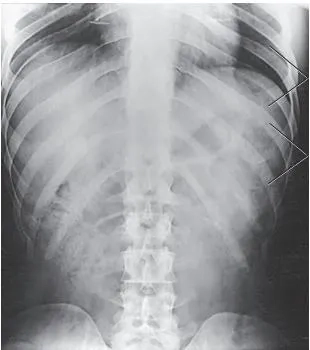
\includegraphics[width=0.7\linewidth]{imagenes/costillas infra}
		\caption[]{Arcos costales infra diafragmaticos}
		\label{fig:costillas-infra}
	\end{figure*}
	
\clearpage
	%----------------------------------------------------------
	%  Para agregar otro enfoque duplicá el bloque
	%  desde \subsection hasta \textbf{Trucos}
	%----------------------------------------------------------


%%%%%%%%%%%%%%%%%%%%%%%%%%%%%%%%%%%%%%%%%%%%%%%%%%%%%%%%%%%
%  SECCIÓN: Parrilla Costal
%  Archivo: secciones/parrilla_costal.tex
%  Sin preámbulo ni \begin{document} — lo maneja main.tex
	%%%%%%%%%%%%%%%%%%%%%%%%%%%%%%%%%%%%%%%%%%%%%%%%%%%%%%%%%%%
	
	\section{Tórax}
	
	\subsection{Parrilla Costal - Oblicua Anterior PA - Porción Axilar (OAD / OAI)}
	
	\subsubsection*{1. Identificación}
	
	\textbf{Tipo:} Proyección complementaria. Forma par según el lado afectado:
	\textbf{OAI} (hombro anterior izquierdo apoyado) para desplegar la curva axilar
	\textbf{derecha}; \textbf{OAD} (hombro anterior derecho apoyado) para visualizar las
	porciones medias y anteriores del lado \textbf{derecho}. Se realizan siempre luego
	de la radiografía de tórax PA estándar a 1{,}80~m, cuyo objetivo es descartar
	neumotórax, hemotórax o hemoneumotórax y priorizar el hemitórax a estudiar.
	
	\textbf{Indicaciones clínicas principales:}
	\begin{itemize}
		\item Golpe en el borde axilar del tórax.
		\item Lesiones, fisuras o traumatismo costal con dolor localizado post-trauma.
		\item Puntada o dolor en el costado de origen traumático.
	\end{itemize}
	
	\subsubsection*{2. Técnica Base}
	
	\textbf{Receptor de imagen:} 35 $\times$ 43~cm. Orientación \textbf{longitudinal}
	(eje mayor del receptor paralelo al eje mayor de la región costal).
	
	\textbf{DFRI:} \textbf{100~cm} (1~metro). Distancia estándar para radiografía
	costal oblicua.
	
	\textbf{Técnica:} Básica o intermedia con \textbf{interés óseo}. Se utiliza
	\textbf{bajo kVp} para obtener alto contraste, permitiendo visualizar las
	costillas de extremo a extremo con su cortical ósea sin que el contraste del
	aire pulmonar enmascare posibles fisuras o fracturas.
	
	\textbf{Factores técnicos:} kVp \textbf{bajo} (técnica de alto contraste) ---
	mAs según espesor del hemitórax. El espesor se mide en la región de interés.
	
	\textbf{Bucky:} Bucky de pared con grilla. Se utiliza por el espesor de la
	región y para reducir la radiación dispersa.
	
	\subsubsection*{3. Posicionamiento}
	
	\paragraph{Paciente}
	De pie (bipedestación) en posición PA frente al Bucky de pared, o en decúbito
	semiprono si el paciente no puede estar de pie. El \textbf{lado afectado se
		aleja del receptor} a 45\textdegree. El paciente mira hacia adelante durante
	toda la exposición.
	
	\begin{figure}[h]
		\centering
		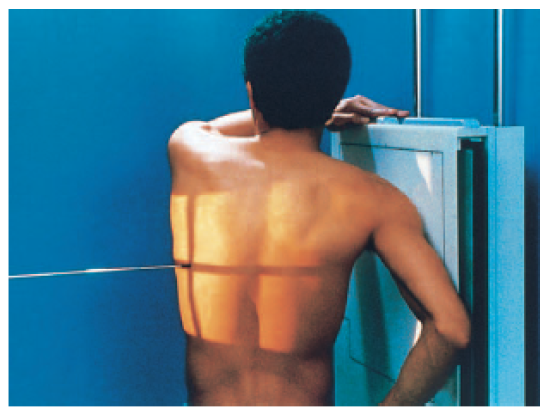
\includegraphics[width=0.7\linewidth]{imagenes/OA costillas}
		\caption{OAD}
		\label{fig:oa-costillas}
	\end{figure}
	
	\begin{figure}
		\centering
		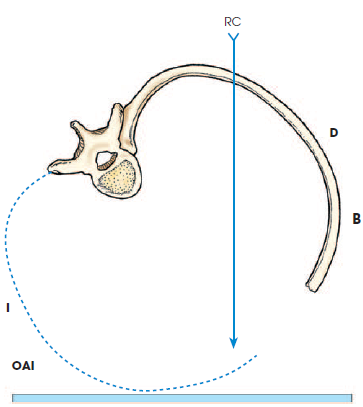
\includegraphics[width=0.7\linewidth]{imagenes/OA1}
		\caption{}
		\label{fig:oa1}
	\end{figure}
	
	
	
	\paragraph{Región de interés}
	Rotación del cuerpo de \textbf{45\textdegree} respecto al plano del receptor:
	\begin{itemize}
		\item \textbf{OAI:} hombro anterior \textbf{izquierdo} apoyado contra el RI;
		el lado afectado (derecho) queda alejado a 45\textdegree. El brazo
		izquierdo (lado apoyado) con el codo flexionado y la mano sobre la
		cadera con la palma hacia afuera. El brazo derecho (lado alejado)
		elevado hasta la altura del hombro o tomado a la parte superior del
		Bucky para no tapar los pulmones.
		\item \textbf{OAD:} hombro anterior \textbf{derecho} apoyado contra el RI;
		el lado afectado (izquierdo) queda alejado a 45\textdegree. El brazo
		derecho (lado apoyado) con el codo flexionado y la mano sobre la
		cadera con la palma hacia afuera. El brazo izquierdo (lado alejado)
		elevado hasta la altura del hombro o tomado a la parte superior del
		Bucky.
	\end{itemize}
	
	\paragraph{Rayo Central}
	Perpendicular al plano del receptor. Punto de entrada: \textbf{T7}, equivalente
	a \textbf{8--10~cm por debajo de la escotadura yugular} (por debajo del nivel
	de la vértebra prominente C7).
	
	\paragraph{Receptor de imagen}
	El borde superior del receptor se coloca \textbf{4~cm por encima del borde
		superior del hombro}. La región a incluir abarca el \textbf{hemitórax de
		interés desde los vértices costales hasta los ángulos costofrénicos}.
	
	\paragraph{Respiración}
	\begin{itemize}
		\item \textbf{Costillas supra-diafragmáticas:} suspensión al final de una
		\textbf{inspiración profunda}, para descender el diafragma y liberar
		los arcos costales superiores.
		\item \textbf{Costillas infra-diafragmáticas:} suspensión al final de una
		\textbf{espiración profunda}, para elevar el diafragma y descubrir
		los arcos costales inferiores.
	\end{itemize}
	
	\subsubsection*{4. Anatomía Visible}
	
	Porción axilar de las costillas del hemitórax de interés desplegada y libre de
	superposición. Las costillas son visibles \textbf{a través del pulmón o del
		abdomen} según la región estudiada (supra o infra-diafragmática). La columna
	vertebral queda separada del borde lateral costal, generando una \textbf{doble
		distancia} entre la columna y el borde lateral de las costillas del lado
	afectado respecto al lado contralateral.
	
	\begin{itemize}
		\item \textbf{OAI:} despliega la curva axilar y los arcos costales anteriores
		\textbf{derechos}.
		\item \textbf{OAD:} visualiza las porciones \textbf{medias y anteriores del
			lado derecho} con mayor nitidez para la búsqueda de fracturas.
	\end{itemize}
	
	\subsubsection*{5. Criterios de Evaluación}
	
	\textbf{Posicionamiento correcto:} La porción axilar de las costillas del lado
	afectado se observa libre de superposición y desplegada. Distancia doble entre
	la columna vertebral y el borde lateral costal del lado afectado en comparación
	con el lado contralateral. Para costillas supra-diafragmáticas: se visualizan
	\textbf{8--9 arcos costales posteriores} por encima del diafragma y las
	costillas anteriores de la 5.ª a la 7.ª en su totalidad por encima del
	diafragma.
	
	\textbf{Ausencia de rotación:} A nivel de la columna, las bases de los cuerpos
	vertebrales presentan \textbf{un único borde}, lo que confirma que la rotación
	no supera los 45\textdegree. Si se visualiza doble borde en los cuerpos
	vertebrales, el paciente está rotado más de 45\textdegree (casi de perfil).
	
	\textbf{Penetración y contraste:} Las costillas se visualizan con su
	\textbf{cortical ósea nítida} a través del parénquima pulmonar o del abdomen.
	El alto contraste obtenido con bajo kVp permite identificar fisuras o fracturas
	sin que el contraste del aire enmascare los detalles óseos.
	
	\subsubsection*{6. Puntos Críticos}
	
	\textbf{Exceso de rotación ($>$45\textdegree):} El paciente queda casi de perfil.
	Radiológicamente se identifica porque las bases de los cuerpos vertebrales
	presentan \textbf{doble borde}. Corrección: verificar que el plano medio sagital
	forme exactamente 45\textdegree con el receptor antes de exponer.
	
	\textbf{Brazo del lado alejado mal posicionado:} El húmero y la escápula
	proyectan \textbf{demasiado hacia arriba} sobre el campo de interés porque el
	paciente no levantó el brazo ni lo alejó correctamente del cuerpo. Corrección:
	indicar al paciente que eleve el brazo hasta la altura del hombro o que lo
	apoye en la parte superior del Bucky de pared.
	
	\textbf{Adaptaciones:} En pacientes con trauma agudo que no toleran la
	bipedestación, realizar la proyección en \textbf{decúbito semiprono} con el
	mismo criterio de rotación de 45\textdegree. Ajustar la técnica si el paciente
	usa inmovilizador costal.
	
	\textbf{Trucos:}
	\begin{itemize}
		\item La nomenclatura de las oblicuas se da por el lado que \textbf{pega}
		contra el receptor, no por el lado afectado: recordar siempre que para
		ver un lado se apoya el \textbf{lado contrario}.
		\item Para la porción anterior y medial de los arcos costales, la oblicua
		estándar es insuficiente: se debe agregar una \textbf{segunda oblicua
			del mismo lado afectado} (acercando el lado afectado al receptor).
		\item Siempre anteceder las oblicuas con la \textbf{Rx de tórax PA a
			1{,}80~m} para descartar complicaciones pleuropulmonares antes de
		focalizar en la parrilla costal.
	\end{itemize}
	
\begin{figure*}
	\centering
	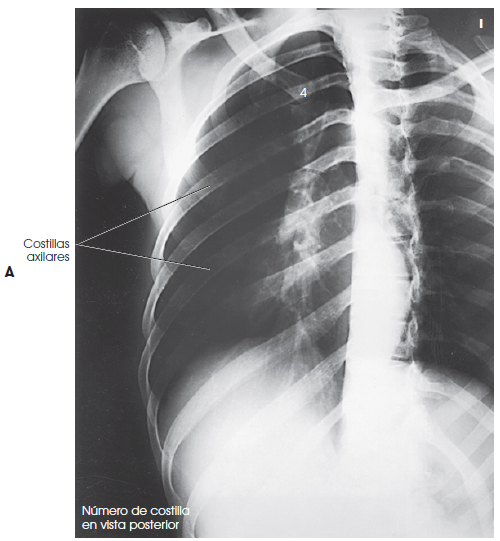
\includegraphics[width=0.7\linewidth]{imagenes/OA2}
	\caption{OAI - OPD}
	\label{fig:oa2}
\end{figure*}

\clearpage

%%%%%%%%%%%%%%%%%%%%%%%%%%%%%%%%%%%%%%%%%%%%%%%%%%%%%%%%%%%
%  SECCIÓN: Parrilla Costal — Oblicuas Posteriores
%  Archivo: secciones/torax.tex
%  Sin preámbulo ni \begin{document} — lo maneja main.tex
	%%%%%%%%%%%%%%%%%%%%%%%%%%%%%%%%%%%%%%%%%%%%%%%%%%%%%%%%%%%
	
	\section{Tórax}
	
	\subsection{Parrilla Costal - Oblicua Posterior AP - Porción Axilar (OPD / OPI)}
	
	\subsubsection*{1. Identificación}
	
	\textbf{Tipo:} Proyección complementaria. Forma par con las oblicuas anteriores (OAD / OAI) para completar el estudio de la parrilla costal.
	
	\textbf{Indicaciones clínicas principales:}
	\begin{itemize}
		\item Traumatismo costal con dolor axilar y/o posterior (ej.: caída de costado hacia atrás).
		\item Sospecha de fractura costal en arcos posteriores o borde axilar.
		\item Lesiones costales no visualizadas en la proyección PA estándar.
		\item Siempre complementar con radiografía de tórax PA estándar previa para descartar neumotórax, hemotórax o hemoneumotórax.
	\end{itemize}
	
	\subsubsection*{2. Técnica Base}
	
	\textbf{Receptor de imagen:} $35 \times 43$ cm. Orientación \textbf{longitudinal} (eje mayor vertical) en relación al eje mayor de la región.
	
	\textbf{DFRI:} 100 cm (1 metro).
	
	\textbf{Técnica:} Básica o intermedia para paciente estándar.
	
	\textbf{Factores técnicos:} kVp y mAs según técnica básica / intermedia según biotipo del paciente.
	
	\textbf{Bucky:} Sí, con grilla.
	
	\subsubsection*{3. Posicionamiento}
	
	\paragraph{Paciente}
	De pie (bipedestación) o en decúbito supino. El \textbf{lado afectado} se apoya contra el receptor de imagen. El plano medio sagital forma un ángulo de \textbf{45°} con respecto al plano del receptor.
	
	\paragraph{Región de interés}
	Se rota el cuerpo 45° sobre su eje longitudinal, de modo que el \textbf{hombro posterior del lado afectado} quede en contacto con el receptor:
	\begin{itemize}
		\item \textbf{OPD} (Oblicua Posterior Derecha): se acerca el lado derecho al receptor; el hombro posterior derecho apoya contra el RI. Se utiliza para visualizar los arcos costales posteriores \textbf{derechos}.
		\item \textbf{OPI} (Oblicua Posterior Izquierda): se acerca el lado izquierdo al receptor; el hombro posterior izquierdo apoya contra el RI. Se utiliza para visualizar los arcos costales posteriores \textbf{izquierdos} y el borde axilar izquierdo.
	\end{itemize}
	El \textbf{brazo del lado afectado} (más cercano al receptor) se levanta con la mano apoyada sobre la cabeza, para retirar la escápula del campo de interés. El \textbf{brazo contralateral} se abduce con la mano apoyada en la cadera.
	
	\begin{figure}[h]
		\centering
		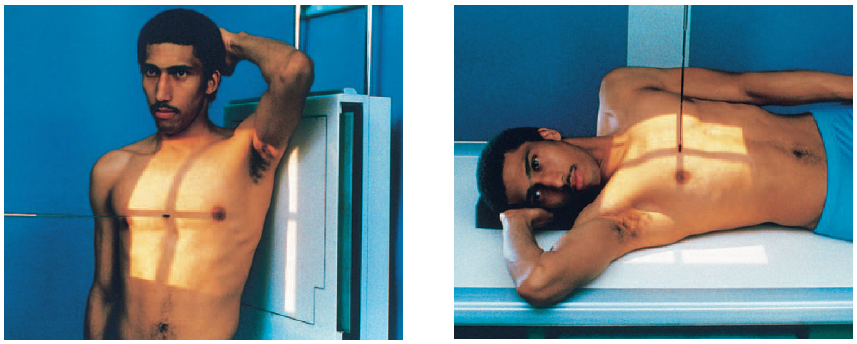
\includegraphics[width=0.7\linewidth]{imagenes/OP1}
		\caption{}
		\label{fig:op1}
	\end{figure}
	
	\begin{figure}
		\centering
		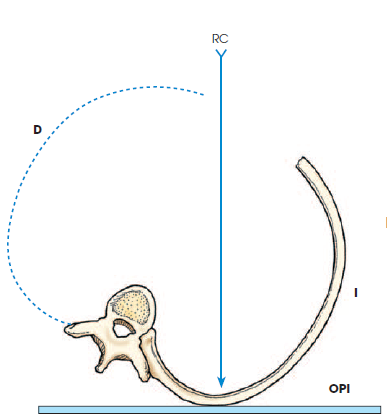
\includegraphics[width=0.7\linewidth]{imagenes/OP3}
		\caption{OP}
		\label{fig:op3}
	\end{figure}
	
	
	\paragraph{Rayo Central}
	Perpendicular al plano del receptor. Punto de entrada: \textbf{T7} (a nivel de la séptima vértebra torácica), centrado en la mitad de la región de interés.
	
	\paragraph{Receptor de imagen}
	El borde superior del receptor se coloca \textbf{2 cm por encima de la vértebra prominente} (C7). De este modo se incluye la totalidad de los arcos costales de interés.
	
	\paragraph{Respiración}
	\begin{itemize}
		\item \textbf{Costillas supradiafragmáticas:} suspensión al final de una \textbf{inspiración profunda} (desciende el diafragma, se liberan las costillas superiores).
		\item \textbf{Costillas infradiafragmáticas:} suspensión al final de una \textbf{espiración profunda} (asciende el diafragma, permitiendo visualizar las costillas bajas sin superposición).
	\end{itemize}
	
	\subsubsection*{4. Anatomía Visible}
	
	Porción axilar de los arcos costales del lado afectado, libre de superposición y elongada. Arcos costales posteriores del hemitórax correspondiente (OPD para arcos derechos, OPI para arcos izquierdos). Las costillas deben ser visibles a través del parénquima pulmonar (región supradiafragmática) o a través del abdomen (región infradiafragmática) según la zona de estudio. Perfil de la tráquea rellena de aire como referencia de posicionamiento. Columna vertebral separada de la región de interés por la rotación de 45°.
	
	\subsubsection*{5. Criterios de Evaluación}
	
	\textbf{Posicionamiento correcto:} La porción axilar de las costillas del lado afectado aparece libre de superposición y alargada. La distancia entre la columna vertebral y el borde lateral de las costillas del lado afectado es aproximadamente el doble que la del lado contralateral. La escápula del lado afectado queda desplazada lateralmente, fuera del campo costal.
	
	\textbf{Ausencia de rotación excesiva:} Si las costillas aparecen acortadas con curvatura cerrada sobre sí mismas, el paciente está demasiado de perfil (más de 45°); se debe reducir la rotación. Si la columna superpone excesivamente el parénquima del lado afectado, la rotación también es excesiva.
	
	\textbf{Penetración y contraste:} Las costillas deben ser visibles tanto en la zona pulmonar como en la zona abdominal según la región estudiada. La técnica básica o intermedia debe garantizar visualización ósea con contraste adecuado.
	
	\subsubsection*{6. Puntos Críticos}
	
	\textbf{Rotación excesiva (más de 45°):} Las costillas se acortan y muestran curvatura cerrada, perdiendo el despliegue axilar buscado. Corrección: reducir el ángulo de rotación hasta 45° o menos.
	
	\textbf{Escápula superpuesta al borde costal externo:} Ocurre cuando el brazo del lado afectado no se levanta correctamente. Corrección: indicar al paciente que eleve el brazo con la mano sobre la cabeza para desplazar lateralmente la escápula fuera del campo.
	
	\textbf{Columna superpuesta al parénquima del lado afectado:} Indica rotación excesiva. Corrección: recolocar el paciente con rotación de 45° o menos.
	
	\textbf{Adaptaciones:} En pacientes con trauma severo o imposibilidad de bipedestación, la proyección puede realizarse en decúbito supino con el lado afectado elevado sobre el receptor. En ese caso, se mantiene la rotación de 45° con apoyo de cuñas o almohadillas radiolúcidas.
	
	\textbf{Trucos:}
	\begin{itemize}
		\item Regla mnemotécnica de nomenclatura: la oblicua se nombra según el lado que \textbf{pega} contra el receptor. OPD = lado derecho pegado al receptor.
		\item Para las oblicuas posteriores, siempre se \textbf{acerca el lado afectado}. Para las anteriores, se \textbf{aleja el lado afectado} (principio inverso).
		\item La OAD es equivalente a la OPI y viceversa (el cuerpo vertebral apunta hacia el mismo lado en ambas).
		\item Verificar la marca del lado en la imagen: debe coincidir con el lado de las apófisis espinosas visibles (OPD/OPI comparten este criterio con OAD/OAI respectivamente).
		\item Siempre comenzar el estudio costal con una PA de tórax a 1,80 m para descartar complicaciones pleurales antes de realizar las oblicuas.
	\end{itemize}
	
	\clearpage
	
	
	\begin{figure*}[h]
		\centering
		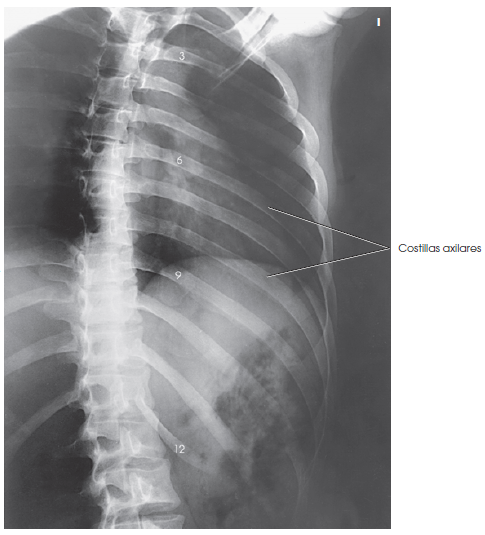
\includegraphics[width=0.7\linewidth]{imagenes/OP2}
		\caption{OPI - OAD}
		\label{fig:op2}
	\end{figure*}


\clearpage

	%----------------------------------------------------------
	%  Para agregar otro enfoque duplicá el bloque
	%  desde \subsection hasta \textbf{Trucos}
	%----------------------------------------------------------
	
\section{Tórax}

\subsection{Proyección Oblicua Anterior Derecha de Esternón (OAD)}

\subsubsection*{1. Identificación}

\textbf{Tipo:} Proyección de elección para el estudio del esternón. Complementa con lateral de esternón cuando se requiere.

\textbf{Indicaciones clínicas principales:}
\begin{itemize}
	\item Fractura esternal (contexto postraumático)
	\item Dolor retroesternal o dolor medio del pecho
	\item Procesos inflamatorios o infecciosos esternales
	\item Control de osteosíntesis esternal
\end{itemize}

\subsubsection*{2. Técnica Base}

\textbf{Receptor de imagen:} 24 × 30 cm. Orientación \textbf{longitudinal} en relación al eje mayor del esternón.

\textbf{DFRI:} 100 cm. Distancia estándar para proyecciones de tórax con Bucky mural.

\textbf{Técnica:} básica o intermedia. Se utiliza \textbf{kVp bajo} para obtener \textbf{alto contraste}, lo que permite resaltar la estructura ósea del esternón a través de la silueta cardiaca, aprovechando la densidad homogénea del mediastino como fondo.

\textbf{Factores técnicos:} kVp \textbf{bajo} --- mAs según espesor del tórax medido a nivel del esternón.

\textbf{Bucky:} sí, se utiliza Bucky con grilla.

\subsubsection*{3. Posicionamiento}

\paragraph{Paciente}
De pie (preferible) o en semidecúbito prono con ligera rotación. Brazo derecho al lado del cuerpo; brazo izquierdo elevado por encima de la cabeza.

\begin{figure}[h]
	\centering
	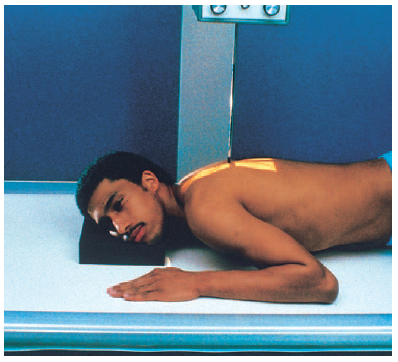
\includegraphics[width=0.7\linewidth]{imagenes/esternon1}
	\caption{}
	\label{fig:esternon1}
\end{figure}



\paragraph{Región de interés}
Paciente rotado \textbf{15 a 20°} hacia el lado derecho, alejando el lado izquierdo del receptor. La rotación varía según biotipo: tórax ancho requiere \textbf{menor} rotación; tórax delgado requiere \textbf{mayor} rotación. Para determinar el grado correcto, se puede colocar una mano sobre el esternón y otra sobre la apófisis espinosa correspondiente.

\paragraph{Rayo Central}
Perpendicular al plano del receptor. Punto de entrada: \textbf{centro del esternón}, a \textbf{2,5 cm a la izquierda de la línea media del paciente}.

\paragraph{Receptor de imagen}
Centrado en el esternón. El borde superior del receptor se ubica \textbf{4 cm por encima de la escotadura yugular} para asegurar la inclusión del manubrio.

\paragraph{Respiración}
Suspendida en \textbf{espiración}. La espiración eleva el diafragma y reduce el campo pulmonar superpuesto, mejorando el contraste sobre el esternón.

\begin{figure}[h]
	\centering
	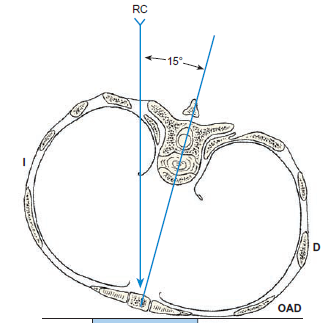
\includegraphics[width=0.7\linewidth]{imagenes/esternon2}
	\caption{}
	\label{fig:esternon2}
\end{figure}


\subsubsection*{4. Anatomía Visible}

Estructuras principales: manubrio, cuerpo y apéndice xifoides del esternón; articulaciones esternoclaviculares; articulaciones costoesternales. El esternón debe proyectarse sobre la silueta cardiaca, libre de superposición de vértebras dorsales. La superposición sobre el mediastino es una ventaja: su densidad homogénea actúa como fondo uniforme que facilita la detección de alteraciones en el contorno y la cortical esternal.

\subsubsection*{5. Criterios de Evaluación}

\textbf{Posicionamiento correcto:} el esternón aparece superpuesto con la silueta cardiaca, sin contacto con las vértebras dorsales. Todo el eje longitudinal, desde el manubrio hasta el xifoides, debe estar visible en la imagen.

\textbf{Ausencia de rotación incorrecta:} el esternón no debe proyectarse sobre el campo pulmonar derecho; si se observa trama pulmonar superpuesta al hueso, la rotación es insuficiente o está invertida.

\textbf{Penetración y contraste:} técnica adecuada cuando el esternón es visible a través de las costillas, el corazón y el pulmón con alto contraste. Un kVp elevado produce escala larga que dificulta la diferenciación de bordes esternales y la detección de trazos de fractura.

\subsubsection*{6. Puntos Críticos}

\textbf{Proyección hacia el campo pulmonar derecho (OAI):} si el esternón se superpone con el parénquima pulmonar derecho, la trama vascular puede simular fracturas o lesiones óseas, con especial riesgo en pacientes añosos y fumadores. Siempre proyectar hacia la silueta cardiaca izquierda.

\textbf{Rotación insuficiente o excesiva:} la rotación insuficiente superpone el esternón sobre la columna vertebral; la excesiva lo desplaza hacia el pulmón derecho. El rango de \textbf{15 a 20°} debe ajustarse al biotipo.

\textbf{Adaptaciones:} para paciente politraumatizado que no puede oblicuarse, se realiza una \textbf{OPI en decúbito supino} angulando el RC \textbf{15 a 20° hacia el lado izquierdo}. La imagen tiene menor fidelidad diagnóstica; se valoran el contorno esternal y la integridad de la cortical.

\textbf{Trucos:} el esternón es un órgano hematopoyético y radiosensible; la OAD lo aleja de la fuente, reduciendo la dosis respecto a la OAI y produciendo menor magnificación geométrica.

\begin{figure*}[h]
	\centering
	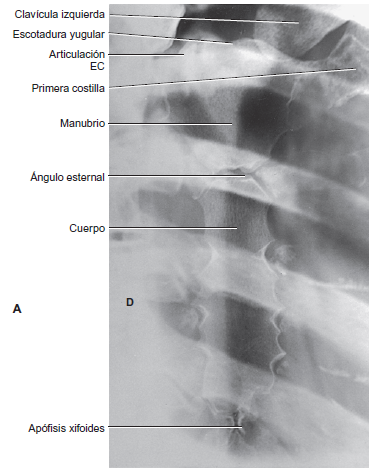
\includegraphics[width=0.7\linewidth]{imagenes/esternon3}
	\caption{OAD esternón}
	\label{fig:esternon3}
\end{figure*}

\clearpage

%%%%%%%%%%%%%%%%%%%%%%%%%%%%%%%%%%%%%%%%%%%%%%%%%%%%%%%%%%%
%  SECCIÓN: Esternón
%  Archivo: secciones/esternon.tex
%  Sin preámbulo ni \begin{document} — lo maneja main.tex
	%%%%%%%%%%%%%%%%%%%%%%%%%%%%%%%%%%%%%%%%%%%%%%%%%%%%%%%%%%%
	
	\section{Tórax}
	
	\subsection{Proyección Lateral de Esternón}
	
	\subsubsection*{1. Identificación}
	
	\textbf{Tipo:} Proyección complementaria del esternón. Forma par con la OAD de esternón.
	
	\textbf{Indicaciones clínicas principales:}
	\begin{itemize}
		\item Fractura esternal (contexto postraumático)
		\item Dolor retroesternal o dolor medio del pecho
		\item Procesos inflamatorios o infecciosos esternales
		\item Control de osteosíntesis esternal
	\end{itemize}
	
	\subsubsection*{2. Técnica Base}
	
	\textbf{Receptor de imagen:} 24 × 30 cm. Orientación \textbf{longitudinal} en relación al eje mayor del esternón.
	
	\textbf{DFRI:} 140 a 180 cm. La distancia aumentada compensa la magnificación geométrica producida por la mayor distancia entre el esternón y el receptor en posición lateral.
	
	\textbf{Técnica:} intermedia. El esternón es un hueso plano, subcutáneo y rodeado de partes blandas y aire; se utiliza únicamente el espesor del esternón como referencia de medición. Se busca \textbf{máximo contraste óseo}.
	
	\textbf{Factores técnicos:} kVp \textbf{intermedio} --- mAs según espesor medido exclusivamente a nivel del esternón.
	
	\textbf{Bucky:} sí, se utiliza Bucky con grilla.
	
	\subsubsection*{3. Posicionamiento}
	
	\paragraph{Paciente}
	De pie (preferible) o en decúbito lateral. En bipedestación, el hombro del lado estudiado apoyado contra el receptor. Plano medio sagital paralelo al receptor de imagen.
	
	\paragraph{Región de interés}
	\textbf{En bipedestación --- posición de himno:} se instruye al paciente a sacar el pecho, llevar los brazos y hombros hacia atrás y entrelazar las manos por detrás de la espalda. Esta maniobra proyecta el esternón anteriormente, separándolo de las estructuras posteriores y reduciendo la superposición de costillas.
	
	\textbf{En decúbito lateral:} paciente recostado sobre un lado, brazos elevados por encima de la cabeza, hombros llevados hacia atrás. Posición lateral estricta, sin rotación.
	
	\paragraph{Rayo Central}
	Perpendicular al plano del receptor. Punto de entrada: \textbf{borde lateral del esternón a nivel de su zona media}.
	
	\paragraph{Receptor de imagen}
	Centrado en el esternón. El borde superior del receptor se ubica \textbf{4 cm por encima de la escotadura yugular} para incluir el manubrio. Colimar a los cuatro lados del área esternal.
	
	\paragraph{Respiración}
	Suspendida en \textbf{inspiración}. Al inspirar, los pulmones se llenan de aire y el esternón se desplaza anteriormente, mejorando su separación de las estructuras posteriores y aumentando el contraste.
	
	\subsubsection*{4. Anatomía Visible}
	
	Todo el esternón en perfil: manubrio, cuerpo y apéndice xifoides, desde la escotadura yugular hasta el extremo inferior del xifoides. El esternón debe visualizarse libre de superposición de costillas y con mínima superposición de partes blandas. No es una imagen de alta fidelidad diagnóstica; su valor principal reside en la evaluación del contorno anterior y posterior del hueso.
	
	\subsubsection*{5. Criterios de Evaluación}
	
	\textbf{Posicionamiento correcto:} todo el eje longitudinal del esternón visible desde el manubrio hasta el xifoides, sin superposición de costillas.
	
	\textbf{Ausencia de rotación:} el esternón se proyecta en perfil estricto; cualquier rotación del tronco superpone estructuras costales sobre el cuerpo esternal.
	
	\textbf{Penetración y contraste:} bordes óseos nítidos con máximo contraste. La nitidez de los bordes confirma además la ausencia de movimiento durante la exposición. Mínima superposición de partes blandas sobre la cortical esternal.
	
	\subsubsection*{6. Puntos Críticos}
	
	\textbf{Magnificación por distancia objeto-receptor:} en posición lateral el esternón queda alejado del receptor. Si no se compensa aumentando la DFRI a \textbf{140--180 cm}, se produce magnificación significativa que distorsiona la imagen y dificulta la evaluación de trazos de fractura.
	
	\textbf{Rotación del paciente:} cualquier rotación del tronco superpone las costillas sobre el esternón, oscureciendo el contorno óseo. La posición de himno en bipedestación es la principal herramienta para evitar este error.
	
	\textbf{Adaptaciones:} en paciente que no puede estar de pie se utiliza el \textbf{decúbito lateral} con brazos elevados y hombros hacia atrás. La calidad de imagen es comparable si se mantiene la posición lateral estricta.
	
	\textbf{Trucos:} medir el espesor únicamente a nivel del esternón y no del tórax completo para evitar sobreexposición. Esta proyección tiene limitaciones diagnósticas inherentes a su geometría y debe interpretarse siempre en conjunto con la OAD.
	
	%----------------------------------------------------------
	%  Para agregar otro enfoque duplicá el bloque
	%  desde \subsection hasta \textbf{Trucos}
	%----------------------------------------------------------
	\input{secciones/Vias Aereas}
	\clearpage
\onecolumn
\thispagestyle{empty}
\vspace*{\fill}
\begin{center}
	{\color{radblue}\rule{\linewidth}{2pt}}\par
	\vspace{6mm}
	{\Huge\bfseries\color{radblue} Mamografía}\par
	\vspace{6mm}
	{\color{radblue}\rule{\linewidth}{2pt}}
\end{center}
\vspace*{\fill}
\clearpage
\twocolumn
\pagestyle{contenido}

%%%%%%%%%%%%%%%%%%%%%%%%%%%%%%%%%%%%%%%%%%%%%%%%%%%%%%%%%%%
%  SECCIÓN: Mamografía
%  Archivo: secciones/mamografia.tex
%  Sin preámbulo ni \begin{document} — lo maneja main.tex
	%%%%%%%%%%%%%%%%%%%%%%%%%%%%%%%%%%%%%%%%%%%%%%%%%%%%%%%%%%%
	
	\section{Mamografía}
	
	\subsection{Introducción a la Mamografía}
	
	\subsubsection*{1. Definición y Rol Clínico}
	
	\textbf{Técnica:} Principal método de estudio de la mama mediante imagen. Técnica de elección para la detección precoz del cáncer de mama.
	
	\textbf{Alcance diagnóstico:} La mamografía \textbf{no diagnostica} el cáncer de mama. El diagnóstico definitivo requiere confirmación anatomopatológica mediante biopsia del tejido de la lesión.
	
	\textbf{Comunicación con el paciente:} Siempre transmitir el mensaje con claridad, reducir el miedo y promover activamente la prevención.
	
	\subsubsection*{2. Anatomía de la Mama}
	
	\paragraph{Estructura general}
	Glándula lobulada de forma hemisférica, constituida por estroma fibroso con tejido adiposo. Se localiza en la aponeurosis superficial de la región anterolateral del tórax, tanto femenino como masculino. Presenta una prolongación axilar denominada \textbf{cola de Spence}, zona de ganglios linfáticos con relevancia oncológica.
	
	
	\paragraph{Organización glandular}
	La mama femenina adulta consta de \textbf{15 a 20 lóbulos}, cada uno subdividido en lobulillos individuales. Estos contienen los elementos glandulares denominados \textbf{acinos} o \textbf{ULDT} (Unidades Lobulillares Ductales Terminales), estructuras de importancia clínica por ser origen frecuente de carcinomas. Los conductos desembocan en el pezón.
	
	\paragraph{Ligamentos de Cooper}
	Las mamas están sujetas por los \textbf{ligamentos de Cooper}. La firmeza o flacidez de la mama depende del estado de estos ligamentos y del contenido relativo de tejido adiposo.
	
	\subsubsection*{3. Clasificación por Tipo de Mama}
	
	\paragraph{Mama A — Adiposa}
	Totalmente grasa. Radiolúcida (hipodensa). Presente en pacientes post-menopausia, mamas infantiles y masculinas. Requiere menor compresión.
	
	\paragraph{Mama B — Fibrosa / Densa}
	Predominio de tejido fibroso. Mayor densidad radiológica.
	
	\paragraph{Mama C — Heterogéneamente Densa}
	Densidad heterogénea. Fibroglandular. Requiere estudio complementario con ecografía. Mayor propensión a desarrollar cáncer.
	
	\paragraph{Mama D — Muy Densa / Fibroglandular}
	Hiperdensa, de mayor complejidad diagnóstica. Presente en pacientes post-pubertad hasta los 30 años, embarazadas, período de lactancia y por condicionamiento genético. La compresión puede resultar molesta. Requiere ecografía complementaria obligatoria. Mayor propensión a desarrollar cáncer.
	
	\subsubsection*{4. Signos Clínicos a Identificar}
	
	Al realizar el estudio, registrar y describir toda señal visible. Los principales signos a identificar son:
	
	\begin{itemize}
		\item Engrosamiento de la piel
		\item Secreción del pezón (acuosa, láctea o hemática), unilateral o bilateral
		\item Dilatación venosa superficial
		\item Hundimiento o retracción del pezón
		\item Protuberancia o masa palpable
		\item Cambio de forma o tamaño
		\item Costras en el pezón
		\item Piel de naranja (signo de edema dérmico con aspecto punteado)
	\end{itemize}
	

	
	\subsubsection*{5. Sistema BI-RADS}
	
	\textbf{Definición:} Sistema estandarizado de categorización de hallazgos mamográficos. Escala del \textbf{0 al 6}.
	
	\textbf{Categorías:}
	
	\begin{itemize}
		\item \textbf{0} — Estudio insuficiente. Se recomienda correlación con otro método de imagen.
		\item \textbf{1 y 2} — Benigno. Sin hallazgos significativos o hallazgo con características benignas definidas.
		\item \textbf{3} — Intermedio. Lesión con apariencia de benignidad; requiere control evolutivo cada 6 meses.
		\item \textbf{4} — Sospecha moderada. Subcategorías A, B y C según grado de sospecha.
		\item \textbf{5} — Altamente sospechoso de malignidad.
		\item \textbf{6} — Malignidad confirmada (diagnóstico histológico previo).
	\end{itemize}
	
	\subsubsection*{6. Consideraciones Clínicas Relevantes}
	
	\textbf{Límite diagnóstico:} La mamografía detecta lesiones pero no las diagnostica. Toda categoría BI-RADS 4 o superior requiere derivación para biopsia.
	
	\textbf{Mamas densas (C y D):} Reducen la sensibilidad de la mamografía por enmascaramiento de lesiones. La ecografía complementaria es obligatoria en estos casos.
	
	\textbf{Cola de Spence:} Zona axilar de la mama con presencia de ganglios linfáticos. Área de relevancia oncológica; puede ser asiento de metástasis ganglionares.
	
	\textbf{Prevención:} Promover activamente el control mamográfico periódico. La detección precoz modifica significativamente el pronóstico.
	
\clearpage
\onecolumn

\begin{figure}[]
	\centering
	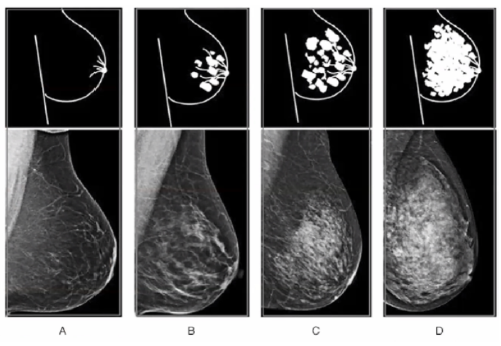
\includegraphics[width=0.5\linewidth]{imagenes/mamo1}
	\caption[]{Tipos de mama}
	\label{fig:mamo1}
\end{figure}

	\begin{figure}[]
	\centering
	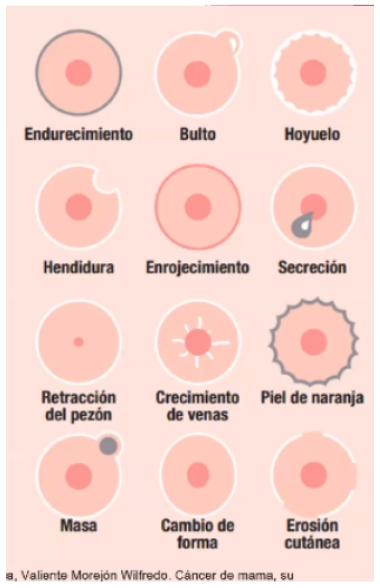
\includegraphics[width=0.40\linewidth]{imagenes/mamo2}
	\caption{Signos clínicos}
	\label{fig:mamo2}
\end{figure}

\twocolumn
\clearpage
	
	%----------------------------------------------------------
	%  Para agregar otro enfoque duplicá el bloque
	%  desde \subsection hasta \textbf{Trucos}
	%----------------------------------------------------------
	
	
%%%%%%%%%%%%%%%%%%%%%%%%%%%%%%%%%%%%%%%%%%%%%%%%%%%%%%%%%%%
%  SECCIÓN: Mamografía
%  Archivo: secciones/mamografia.tex
%  Sin preámbulo ni \begin{document} — lo maneja main.tex
	%%%%%%%%%%%%%%%%%%%%%%%%%%%%%%%%%%%%%%%%%%%%%%%%%%%%%%%%%%%
	
	\section{Mamografia}
	
	\subsection{Proyección Cráneo-Caudal (CC) Der / Izq}
	
	\subsubsection*{1. Identificación}
	
	\textbf{Tipo:} Proyección básica de mamografía. Forma par con la proyección oblicua mediolateral (OML).
	
	\textbf{Indicaciones clínicas principales:}
	\begin{itemize}
		\item Detección y evaluación de calcificaciones, quistes y carcinomas
		\item Identificación de otras anomalías o cambios del tejido mamario
		\item Estudio de nódulos palpables
		\item Estudio bilateral de rutina (screening o diagnóstico)
	\end{itemize}
	
	\subsubsection*{2. Técnica Base}
	
	\textbf{Receptor de imagen:} 18×24 cm o 24×30 cm según el tamaño de la mama. Orientación \textbf{transversal}.
	
	\textbf{DFRI:} \textit{[dato no suministrado]}.
	
	\textbf{Técnica:} Ultra contrastada. La mama está compuesta por tejidos con bajo contraste intrínseco (grasa y glándula son radiológicamente homogéneos); la técnica ultra contrastada --- mediante kVp bajo sumado a la compresión --- genera una escala de grises corta que permite diferenciarlos entre sí.
	
	\textbf{Factores técnicos:} kVp \textbf{\textit{[dato no suministrado]}} --- mAs \textbf{\textit{[dato no suministrado]}}. Espesor medido con la mama comprimida sobre el receptor.
	
	\textbf{Bucky:} Equipo de mamografía con compresor dedicado; grilla específica de mamografía.
	
	\subsubsection*{3. Posicionamiento}
	
	\paragraph{Paciente}
	De pie o sentado, con ambos pies orientados frente al equipo. Brazos relajados a los lados con descenso activo del hombro ipsilateral. Cabeza girada hacia el lado opuesto al seno a estudiar.
	
	\paragraph{Región de interés}
	La mama se coloca sobre el receptor, perpendicular a la caja torácica. Se rota levemente el pezón hasta dejarlo de perfil. Se realiza tracción del tejido mamario hacia el receptor, alejándolo de la pared torácica. El pliegue inframamario se eleva al nivel del borde del receptor.
	
	\paragraph{Rayo Central}
	Perpendicular a la base de la mama (plano horizontal). Punto de entrada: \textbf{base de la mama, a nivel del pliegue inframamario elevado}.
	
	\paragraph{Receptor de imagen}
	Elevado para apoyar el pliegue inframamario. Centrado de forma que incluya todo el parénquima mamario, la grasa retromamaria y, de ser posible, el músculo pectoral mayor en el borde posterior. El pedal del compresor se acciona una vez realizada la tracción y correcta posición de la mama.
	
	\paragraph{Respiración}
	Suspendida (paciente contiene la respiración durante la exposición). Reduce el movimiento y evita artefactos de borrosidad.
	
	\subsubsection*{4. Anatomía Visible}
	
	Parénquima mamario completo en proyección cráneo-caudal. Grasa retromamaria en el borde posterior. Músculo pectoral mayor visible en el margen posterior cuando la tracción y la elevación del pliegue son adecuadas. Pezón de perfil y centrado en el borde anterior. Piel y tejido subcutáneo en los bordes superior e inferior.
	
	\subsubsection*{5. Criterios de Evaluación}
	
	\textbf{Posicionamiento correcto:} Ambas proyecciones CC simétricas entre sí. Pezón de perfil y centrado. Bordes superior e inferior (pliegue inframamario) contenidos dentro del campo. Músculo pectoral mayor visible en el borde posterior. La medida de la PNL en la CC no debe diferir en más de 1 cm respecto a la PNL de la proyección OML del mismo lado.
	
	\textbf{Ausencia de rotación:} Pezón centrado y de perfil; si no está de perfil indica falta de rotación, corregible con rotación externa o interna leve de la mama. Densidad glandular simétrica entre ambas CC; asimetría puede indicar error de posicionamiento o variación anatómica del paciente.
	
	\textbf{Penetración y contraste:} Escala de grises corta que permita diferenciar tejido glandular de tejido graso. Técnica ultra contrastada verificable por la correcta separación tonal entre componentes mamarios.
	
	\subsubsection*{6. Puntos Críticos}
	
	\textbf{Pezón no de perfil:} La rotación insuficiente impide evaluar correctamente el tejido retroareolar; corregir con rotación externa o interna leve antes de comprimir.
	
	\textbf{Tracción insuficiente o elevación incorrecta del pliegue:} El músculo pectoral no se visualiza en el borde posterior y se excluye tejido mamario profundo; realizar nueva tracción activa y elevar correctamente el pliegue inframamario antes de comprimir.
	
	\textbf{Adaptaciones:} \textit{[dato no suministrado]}.
	
	\textbf{Trucos:} Verificar la PNL de la CC contra la PNL de la OML del mismo lado: una diferencia mayor a 1 cm indica pérdida de tejido profundo en alguna de las dos proyecciones y obliga a repetir. La asimetría de densidad entre ambas CC puede deberse a la anatomía del paciente o a un error de posicionamiento encubierto.
	
	\clearpage
	\onecolumn
	
	\begin{figure}
		\centering
		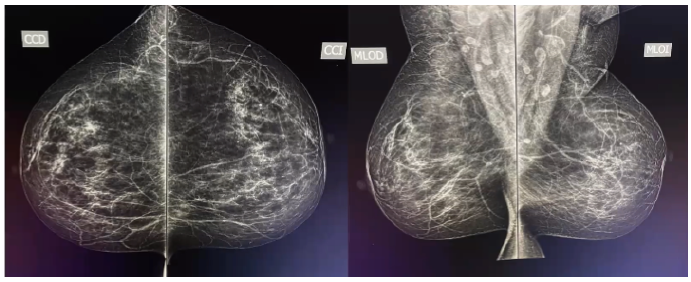
\includegraphics[width=1\linewidth]{imagenes/mamo4}
		\caption{CC: craneo caudal + I o D, MLO: medio lateral oblicua + I o D}
		\label{fig:mamo4}
	\end{figure}
	
	\twocolumn
	\clearpage
	
	%----------------------------------------------------------
	%  Para agregar otro enfoque duplicá el bloque
	%  desde \subsection hasta \textbf{Trucos}
	%----------------------------------------------------------
	
%%%%%%%%%%%%%%%%%%%%%%%%%%%%%%%%%%%%%%%%%%%%%%%%%%%%%%%%%%%
%  SECCIÓN: Mamografía
%  Archivo: secciones/mamografia.tex
%  Sin preámbulo ni \begin{document} — lo maneja main.tex
	%%%%%%%%%%%%%%%%%%%%%%%%%%%%%%%%%%%%%%%%%%%%%%%%%%%%%%%%%%%
	
	\section{Mamografia}
	
	\subsection{Proyección Mediolateral Oblicua (MLO)}
	
	\subsubsection*{1. Identificación}
	
	\textbf{Tipo:} Proyección básica de screening mamográfico. Forma par con la proyección craneocaudal (CC).
	
	\textbf{Indicaciones clínicas principales:}
	\begin{itemize}
		\item Screening mamográfico de rutina
		\item Dolor localizado en mama
		\item Sospecha de lesiones en cuadrantes externos y cara lateral profunda del tejido mamario
	\end{itemize}
	
	\subsubsection*{2. Técnica Base}
	
	\textbf{Receptor de imagen:} 18×24 cm o 24×30 cm. Orientación \textbf{transversal (horizontal)} según el biotipo de la paciente.
	
	\textbf{DFRI:} \textit{[dato no suministrado]}.
	
	\textbf{Técnica:} Bajo kVp para maximizar la visualización de la cola de Spence y los ganglios axilares. Los tejidos mamarios (grasa y glándula) son anatómicamente distintos pero radiológicamente homogéneos; el kVp bajo combinado con la compresión permite diferenciarlos, logrando una imagen ultra contrastada con escala larga pero de corto rango efectivo.
	
	\textbf{Factores técnicos:} kVp \textbf{bajo} --- mAs \textit{[dato no suministrado]}. \textit{[Método de medición del espesor no suministrado]}.
	
	\textbf{Bucky:} \textit{[dato no suministrado]}.
	
	\subsubsection*{3. Posicionamiento}
	
	\paragraph{Paciente}
	De pie; si no es posible, sentada. Cuerpo y cadera oblicuados hacia el equipo. El brazo del lado a estudiar se eleva sobre el soporte del equipo o sobre la cabeza. Hombro, brazo y cuerpo deben estar completamente relajados; se indica a la paciente un movimiento de rotación del húmero para favorecer la relajación del músculo pectoral mayor.
	
	\paragraph{Región de interés}
	Tubo y receptor rotados a 45° (rango aceptable: 30°--60°) a la altura del hueco axilar. La mama se tracciona en sentido anteromedial, alejándola de la pared torácica, y se coloca sobre el soporte del equipo para quedar bien perfilada. El pezón debe quedar de perfil. La compresión debe lograr grosor uniforme desplazando la mama hacia arriba y afuera.
	
	\paragraph{Rayo Central}
	Perpendicular al plano del receptor, sin angulación (RC inmóvil, 0°). Punto de entrada: \textbf{base de la mama al borde de la pared torácica}.
	
	\paragraph{Receptor de imagen}
	Centrado en la base de la mama al borde de la pared torácica, posicionado a 45° a la altura del hueco axilar. Debe incluir toda la mama desde el músculo pectoral mayor hasta el pezón, la cola de Spence y los ganglios axilares.
	
	\paragraph{Respiración}
	Apnea durante la exposición. Evita el movimiento y la borrosidad de las estructuras mamarias.
	
	\subsubsection*{4. Anatomía Visible}
	
	Toda la mama incluyendo tejido glandular y grasa subcutánea. Músculo pectoral mayor con convexidad anterior visible, indicando relajación adecuada del hombro y la axila. Cola de Spence y ganglios axilares. Pezón de perfil. Pliegue inframamario abierto y despejado, sin superposición del abdomen.
	
	\subsubsection*{5. Criterios de Evaluación}
	
	\textbf{Posicionamiento correcto:} Toda la mama incluida desde el músculo pectoral mayor hasta el pezón; cola de Spence y ganglios axilares visibles; pliegue inframamario abierto y libre de superposición abdominal.
	
	\textbf{Ausencia de rotación:} Pezón de perfil; mama desplazada hacia arriba y afuera con grosor uniforme producto de compresión óptima; músculo pectoral mayor con borde convexo anterior.
	
	\textbf{Penetración y contraste:} Imagen ultra contrastada con diferenciación visible entre tejido glandular y grasa, lograda mediante kVp bajo y compresión adecuada.
	
	\subsubsection*{6. Puntos Críticos}
	
	\textbf{Hombro y brazo tensionados:} El músculo pectoral mayor aparece recto o cóncavo en lugar de convexo, reduciendo el tejido mamario incluido. Corrección: indicar rotación activa del húmero antes de la compresión.
	
	\textbf{Mama caída o mal traccionada:} Grosor no uniforme y pliegue inframamario superpuesto al abdomen. Corrección: traccionar la mama en sentido anteromedial antes de aplicar la compresión.
	
	\textbf{Adaptaciones:} Si la paciente no puede estar de pie, realizar la proyección sentada manteniendo la angulación del tubo a 45°. Para movilidad limitada del brazo, ajustar el ángulo del tubo dentro del rango 30°--60°.
	
	\textbf{Trucos:} Colocar el delantal de protección abdominal antes de la exposición. Verificar el pezón de perfil y la convexidad del pectoral como indicadores rápidos de posicionamiento correcto antes de comprimir definitivamente.
	
	\clearpage
	\onecolumn
	\begin{figure}
		\centering
		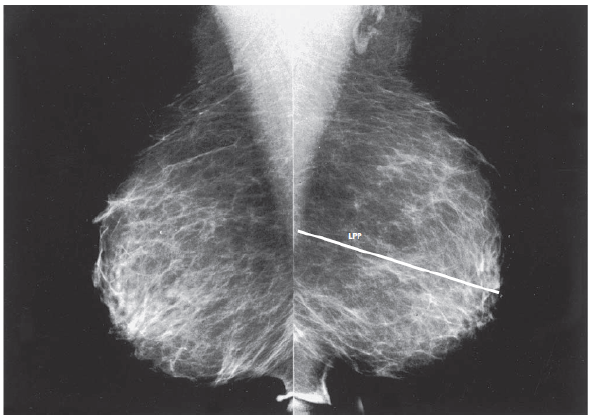
\includegraphics[width=0.7\linewidth]{imagenes/mamo5}
		\caption{Medio Lateral Oblicua}
		\label{fig:mamo5}
	\end{figure}
	\twocolumn
	\clearpage
	%----------------------------------------------------------
	%  Para agregar otro enfoque duplicá el bloque
	%  desde \subsection hasta \textbf{Trucos}
	%----------------------------------------------------------
	
	
	%%%%%%%%%%%%%%%%%%%%%%%%%%%%%%%%%%%%%%%%%%%%%%%%%%%%%%%%%%%
	%  SECCIÓN: [Nombre de la Sección]
	%  Archivo: implante_desplazado_eklund.tex
	%  Sin preámbulo ni \begin{document} — lo maneja main.tex
		%%%%%%%%%%%%%%%%%%%%%%%%%%%%%%%%%%%%%%%%%%%%%%%%%%%%%%%%%%%
		
		\section{Mamografia}
		
		\subsection{Implante Desplazado (ID) — Método de Eklund DC}
		
		\subsubsection*{1. Identificación}
		
		\textbf{Indicaciones clínicas principales:}
		\begin{itemize}
			\item Pacientes con implantes mamarios
			\item Aumento mamario
			\item Fuga intra o extracapsular del implante
		\end{itemize}
		
		\subsubsection*{2. Técnica Base}
		
		\textbf{Receptor de imagen:} 18x24 cm o 24x30 cm.
		
		\textbf{Técnica:} Manual o semiautomática (el equipo no detecta el implante).
		
		\subsubsection*{3. Posicionamiento}
		
		\paragraph{Paciente}
		De pie o sentada en taburete, de cara al portacartuchos. Se realiza tracción hacia atrás contra la pared torácica.
		
		\paragraph{Región de interés}
		El operador se coloca de pie en el lado interno de la mama a explorar. Se levanta el pliegue inframamario. Una vez localizado el borde anterior del implante, se tira con suavidad del tejido mamario anterior hacia el portacartucho. Se debe conseguir una compresión adicional de 2--5 cm con el implante desplazado. Se le pide al paciente que indique si la compresión le resulta incómoda.
		
		\paragraph{Respiración}
		Suspendida (contenida). Se solicita al paciente que aguante la respiración una vez conseguida la compresión completa, momento en el que se realiza la exposición.
		
		\subsubsection*{4. Anatomía Visible}
		
		Tejido mamario anterior y central sin superposición con el implante. Tejido glandular anterior al implante desplazado.
		
		\subsubsection*{5. Criterios de Evaluación}
		
		\textbf{Posicionamiento correcto:} Implante desplazado posteriormente contra la pared torácica. Tejido mamario anterior y central visualizado sin ninguna superposición del implante.
	
	\onecolumn
\begin{figure}
	\centering
	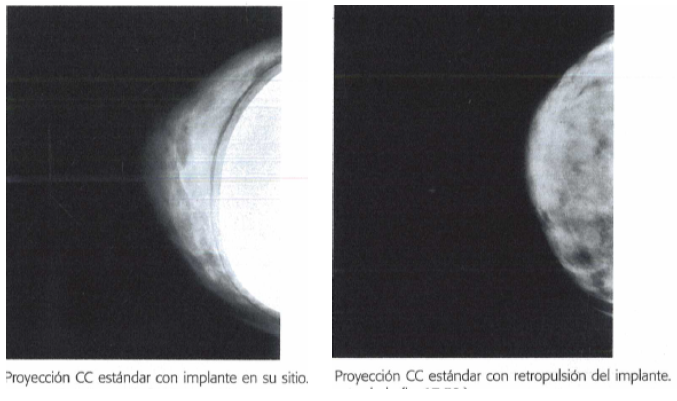
\includegraphics[width=0.7\linewidth]{imagenes/mamo6}
	\caption{}
	\label{fig:mamo6}
\end{figure}

\begin{figure}
	\centering
	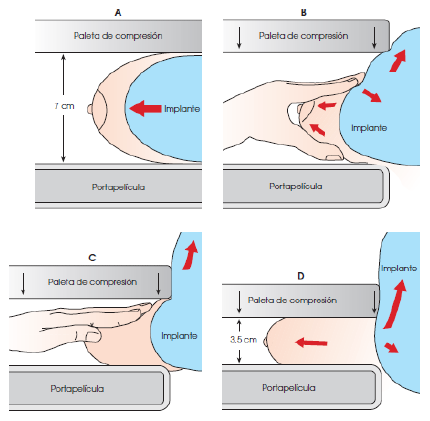
\includegraphics[width=0.7\linewidth]{imagenes/mamo7}
	\caption{}
	\label{fig:mamo7}
\end{figure}

\twocolumn
\clearpage
		
		%----------------------------------------------------------
		%  Para agregar otro enfoque duplicá el bloque
		%  desde \subsection hasta \textbf{Trucos}
		%----------------------------------------------------------
	\clearpage
\onecolumn
\thispagestyle{empty}
\vspace*{\fill}
\begin{center}
	{\color{radblue}\rule{\linewidth}{2pt}}\par
	\vspace{6mm}
	{\Huge\bfseries\color{radblue} Abdomen}\par
	\vspace{6mm}
	{\color{radblue}\rule{\linewidth}{2pt}}
\end{center}
\vspace*{\fill}
\clearpage
\twocolumn
\pagestyle{contenido}


%%%%%%%%%%%%%%%%%%%%%%%%%%%%%%%%%%%%%%%%%%%%%%%%%%%%%%%%%%%
%  SECCIÓN: Abdomen
%  Archivo: secciones/abdomen.tex
%  Sin preámbulo ni \begin{document} — lo maneja main.tex
%%%%%%%%%%%%%%%%%%%%%%%%%%%%%%%%%%%%%%%%%%%%%%%%%%%%%%%%%%%
	
	\section{Abdomen}
	\subsection{Generalidades de Abdomen}
	
	%----------------------------------------------------------
	%  INFORMACIÓN COMPLEMENTARIA GENERAL
	%----------------------------------------------------------
	
	\subsubsection*{División por Cuadrantes}
	
	Dos planos perpendiculares trazados a nivel del ombligo dividen la región en nueve zonas:
	
	\begin{itemize}
		\item \textbf{Hipocondrio derecho:} hígado y vías biliares
		\item \textbf{Epigastrio:} estómago
		\item \textbf{Hipocondrio izquierdo:} bazo
		\item \textbf{Flanco derecho:} colon ascendente
		\item \textbf{Mesogastrio / región umbilical:} intestino delgado
		\item \textbf{Flanco izquierdo:} colon descendente
		\item \textbf{Fosa ilíaca derecha:} ciego y apéndice
		\item \textbf{Hipogastrio:} vejiga urinaria (cuando está llena)
		\item \textbf{Fosa ilíaca izquierda:} colon sigmoideo
	\end{itemize}
	
	\subsubsection*{Repères Anatómicos}
	
	\textbf{Límite superior:} cúpulas diafragmáticas. \\
	\textbf{Límite inferior:} sínfisis del pubis.
	
	\begin{itemize}
		\item \textbf{Apófisis xifoides:} T9--T10
		\item \textbf{Borde costal inferior:} L2--L3
		\item \textbf{Cresta ilíaca:} L4--L5
		\item \textbf{EIAS}
		\item \textbf{Trocánter mayor:} 3--4 cm por encima de la sínfisis púbica
		\item \textbf{Sínfisis del pubis:} unión anterior de ambos huesos pelvianos
		\item \textbf{Tuberosidad isquiática:} 1--4 cm por debajo de la sínfisis del pubis
	\end{itemize}
	
	\subsubsection*{Consideraciones Técnicas Generales}
	
	\textbf{Bajo contraste intrínseco:} estructuras de densidad similar; se usan técnicas más contrastadas (básica o intermedia).
	
	\textbf{Densidades presentes:}
	\begin{itemize}
		\item Aire (tubo digestivo)
		\item Grasa (rodea riñones, músculos psoas)
		\item Agua (vísceras)
		\item Hueso
	\end{itemize}
	
	\textbf{Líneas grasas:} interfase entre densidad de agua y grasa. Su visualización confirma una técnica adecuada. Principales referencias: borde ínfero-externo del hígado, línea de los músculos psoas (desde L1 hasta la pelvis), contorno perirrenal. Si las vísceras no se ven es porque no hay contraste.
	
	\textbf{Movimientos involuntarios:} inevitables; se compensan con tiempos de exposición cortos. kVp no muy altos, especialmente en pacientes con más grasa abdominal (genera radiación dispersa). El paciente debe estar relajado y con la respiración suspendida en espiración: disminuye el aire y el espesor.
	
	\subsubsection*{Preparación del Paciente}
	
	Indispensable para estudios programados. Dieta controlada, laxantes y enemas previos. Elimina gases y materia fecal del tubo digestivo, mejorando la calidad de imagen.
	
	\textbf{Sin preparación:} pacientes con abdomen agudo, sospecha de perforación o provenientes de emergencias.
	
	\subsubsection*{Consideraciones sobre los Enfoques}
	
	La imagen debe abarcar toda la región: desde cúpulas diafragmáticas hasta sínfisis del pubis. Si no es posible en una sola proyección, se realizan dos: una en decúbito supino de sínfisis hacia arriba y otra en bipedestación de cúpulas hacia abajo.
	
	No confundir decúbito lateral (para obtener un frente de abdomen con RC horizontal) con un paciente en decúbito lateral para un perfil.
	
	\subsubsection*{Protocolo Abdomen Agudo}
	
	\textbf{Par estándar:}
	\begin{enumerate}
		\item Frente en decúbito supino
		\item Frente en bipedestación (ortostática)
	\end{enumerate}
	
	Si el paciente no puede pararse: decúbito lateral izquierdo con rayo horizontal, o como complemento un frente de tórax (sentado). El decúbito lateral izquierdo sustituye la bipedestación en pacientes que no pueden deambular; es el más importante para detectar neumoperitoneo.
	
	\textbf{RC en bipedestación:} perpendicular, para no distorsionar los niveles hidroaéreos.
	
	\subsubsection*{Indicaciones por Hallazgo Clínico}
	
	\textbf{Cuerpo extraño:} frente y perfil de abdomen.
	
	\textbf{Niveles hidroaéreos:} de pie (preferible) o decúbito supino frente y perfil. En el perfil el líquido baja y el aire sube.
	
	\textbf{Neumoperitoneo:} complementar con frente de tórax. Paciente de pie o sentado con torso erguido. El aire tiende a ascender a la zona más alta.
	
	\textbf{Abdomen agudo:} AP decúbito supino + AP bipedestación.
	
	\textbf{Trauma abdominal - hallazgos a valorar:}
	\begin{itemize}
		\item Neumoperitoneo: indica perforación de víscera hueca
		\item Borramiento de línea del psoas: asociado a lesiones retroperitoneales
		\item Fracturas costales
	\end{itemize}
	
	%----------------------------------------------------------
	%  Los enfoques se agregan a continuación como \subsection{}
	%----------------------------------------------------------
	
	\clearpage
	
%%%%%%%%%%%%%%%%%%%%%%%%%%%%%%%%%%%%%%%%%%%%%%%%%%%%%%%%%%%
%  SECCIÓN: Abdomen
%  Archivo: secciones/abdomen.tex
%  Sin preámbulo ni \begin{document} — lo maneja main.tex
	%%%%%%%%%%%%%%%%%%%%%%%%%%%%%%%%%%%%%%%%%%%%%%%%%%%%%%%%%%%
	
	\section{Abdomen}
	
	\subsection{Abdomen AP en Decúbito Supino}
	
	\subsubsection*{1. Identificación}
	
	\textbf{Tipo:} Proyección básica. Forma par con la proyección AP en bipedestación.
	
	\textbf{Indicaciones clínicas principales:}
	\begin{itemize}
		\item Obstrucción intestinal y evaluación de niveles hidroaéreos en paciente sin capacidad de bipedestación
		\item Calcificaciones abdominales, ascitis y exploraciones con contraste
		\item Abdomen agudo
	\end{itemize}
	
	\subsubsection*{2. Técnica Base}
	
	\textbf{Receptor de imagen:} 35$\times$43 cm. Orientación \textbf{longitudinal} en todos los biotipos.
	
	\textbf{DFRI:} \textit{[dato no suministrado]}.
	
	\textbf{Técnica:} Intermedia. Las densidades del abdomen son muy homogéneas (bajo contraste intrínseco), por lo que se requiere una escala larga de grises con kVp intermedio para diferenciar el contorno de las vísceras (riñones), tejido adiposo, aire y hueso. En paciente obeso se utiliza técnica básica por el gran espesor y la consecuente mayor radiación dispersa que engrisa la imagen; en paciente pediátrico muy delgado puede homogeneizarse con herramientas de posproceso.
	
	\textbf{Factores técnicos:} kVp \textbf{[valor]} --- mAs \textbf{[valor]}. Medición del espesor a nivel de las crestas iliacas.
	
	\textbf{Bucky:} Bucky de mesa con grilla.
	
	\subsubsection*{3. Posicionamiento}
	
	\paragraph{Paciente}
	Decúbito supino, brazos a los lados del cuerpo, piernas extendidas con soporte bajo las rodillas. Plano medio sagital perpendicular y centrado al receptor. Se puede aplicar tracción desde los tobillos (verificar ausencia de prótesis) o desde los hombros para corregir la alineación vertebral.
	
		
	\begin{figure}[h]
		\centering
		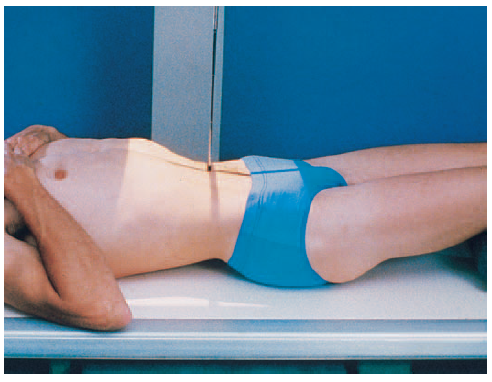
\includegraphics[width=0.7\linewidth]{imagenes/abd2}
		\caption{}
		\label{fig:abd}
	\end{figure}
	
	
	\paragraph{Región de interés}
	Pelvis y abdomen sin rotación: EIAS equidistantes al receptor. El colimador se abre en su totalidad a lo ancho para incluir toda la región abdominal.
	
	\paragraph{Rayo Central}
	Perpendicular al plano del receptor. Punto de entrada: \textbf{a la altura de las crestas iliacas}.
	
	\paragraph{Receptor de imagen}
	Centrado a la altura de las crestas iliacas. El borde inferior debe incluir la sínfisis del pubis; el borde superior debe alcanzar las cúpulas diafragmáticas. Si el paciente es muy alto y no se logra abarcar toda la pelvis, se realiza una segunda exposición centrada en pelvis para incluir la vejiga.
	
	\paragraph{Respiración}
	Al final de la espiración. El descenso del diafragma permite visualizar las estructuras supradiafragmáticas y amplía el campo abdominal visible.

	
	\subsubsection*{4. Anatomía Visible}
	
	Contorno de riñones, borde inferior hepático, músculo psoas bilateral, marco intestinal, columna lumbar y pelvis ósea. Límite superior obligatorio: cúpulas diafragmáticas. Límite inferior obligatorio: sínfisis del pubis. Si alguno de los dos límites queda excluido, la radiografía carece de valor diagnóstico. En decúbito supino los niveles hidroaéreos pueden observarse pero no son tan evidentes como en bipedestación.
	
	\subsubsection*{5. Criterios de Evaluación}
	
	\textbf{Posicionamiento correcto:} Columna vertebral centrada en el receptor; crestas iliacas y cúpulas diafragmáticas incluidas; sínfisis del pubis visible en el borde inferior.
	
	\textbf{Ausencia de rotación:} Espinas iliacas anterosuperiores simétricas; alas iliacas y agujeros obturadores simétricos; apófisis espinosas centradas en los cuerpos vertebrales lumbares; caderas equidistantes a los bordes laterales de la imagen.
	
	\textbf{Penetración y contraste:} Escala larga de grises con kVp intermedio; diferenciación visible entre contorno renal, tejido adiposo perivisceral, gas intestinal y estructuras óseas.
	
	\subsubsection*{6. Puntos Críticos}
	
	\textbf{No incluir la sínfisis del pubis:} La vejiga y el segmento pélvico quedan fuera del campo; ante paciente de gran talla agregar una segunda proyección centrada en pelvis.
	
	\textbf{Rotación de pelvis u hombros:} Genera asimetría de alas iliacas y agujeros obturadores; corregir distribución del peso y alineación del plano sagital antes de la exposición.
	
	\textbf{Adaptaciones:} Si el paciente no puede mantenerse en bipedestación para evaluar aire libre, realizar el enfoque en decúbito lateral izquierdo con RC horizontal como alternativa.
	
	\textbf{Trucos:} La tracción desde los tobillos mejora la alineación vertebral; si hay prótesis en miembros inferiores, traccionar desde los hombros. Si los riñones no son el área de interés, el enfoque puede realizarse en PA estando el paciente de pie para reducir la dosis gonadal.
	
	\clearpage
	\onecolumn
	\begin{figure}
		\centering
		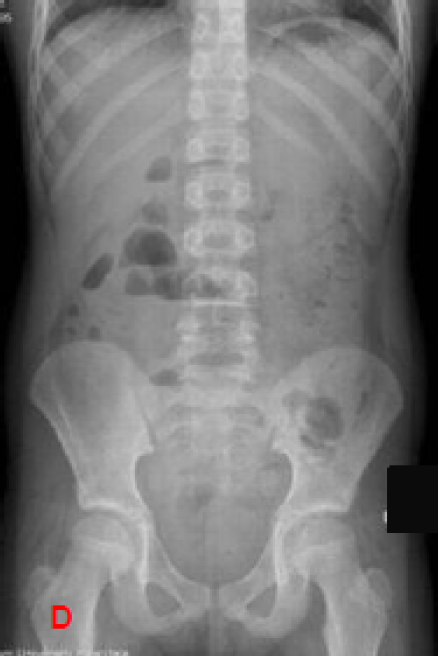
\includegraphics[width=0.7\linewidth]{imagenes/abd4}
		\caption{Desde sínfisis del pubis hacia arriba}
		\label{fig:abd3}
	\end{figure}
	
	\twocolumn
	%----------------------------------------------------------
	\clearpage
	
	\subsection{Abdomen AP en Bipedestación}
	
	\subsubsection*{1. Identificación}
	
	\textbf{Tipo:} Proyección básica. Forma par con la proyección AP en decúbito supino.
	
	\textbf{Indicaciones clínicas principales:}
	\begin{itemize}
		\item Búsqueda de aire libre subdiafragmático (neumoperitoneo)
		\item Obstrucción intestinal con evaluación de niveles hidroaéreos
		\item Abdomen agudo cuando el paciente puede mantenerse en pie
	\end{itemize}
	
	\subsubsection*{2. Técnica Base}
	
	\textbf{Receptor de imagen:} 35$\times$43 cm. Orientación \textbf{longitudinal} en todos los biotipos.
	
	\textbf{DFRI:} \textit{[dato no suministrado]}.
	
	\textbf{Técnica:} Intermedia. Igual justificación que en decúbito: el bajo contraste intrínseco abdominal requiere escala larga de grises con kVp intermedio. En paciente obeso se prefiere técnica básica por la mayor radiación dispersa generada por el gran espesor.
	
	\textbf{Factores técnicos:} kVp \textbf{[valor]} --- mAs \textbf{[valor]}. Medición del espesor a nivel de las crestas iliacas.
	
	\textbf{Bucky:} Bucky mural con grilla.
	
	\subsubsection*{3. Posicionamiento}
	
	\paragraph{Paciente}
	De pie, peso distribuido equitativamente entre ambos pies, brazos a los lados del cuerpo. Plano medio sagital perpendicular y centrado al receptor vertical. Ausencia de rotación de pelvis y hombros.
	
	\begin{figure}
		\centering
		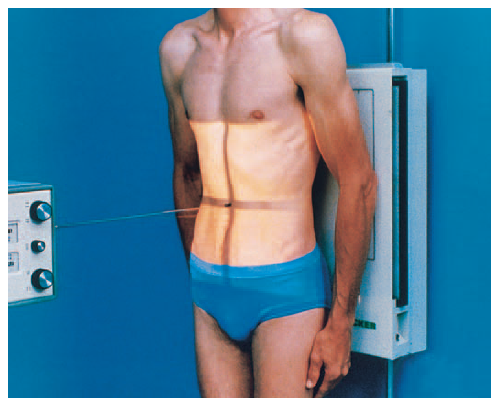
\includegraphics[width=0.7\linewidth]{imagenes/abd}
		\caption{}
		\label{fig:abd}
	\end{figure}
	
	
	\paragraph{Región de interés}
	Abdomen y pelvis sin rotación: EIAS equidistantes al receptor. El colimador se abre en su totalidad a lo ancho para incluir toda la región.
	
	\paragraph{Rayo Central}
	Perpendicular al plano del receptor. Punto de entrada: \textbf{5 cm por encima de las crestas iliacas}, para abarcar las cúpulas diafragmáticas.
	
	\paragraph{Receptor de imagen}
	Centrado por encima del nivel de las crestas iliacas de forma que el borde superior incluya ambas cúpulas diafragmáticas y el borde inferior alcance la sínfisis del pubis. Si el paciente es muy alto, agregar una segunda proyección centrada en pelvis.
	
	\paragraph{Respiración}
	Al final de la espiración. El diafragma desciende, maximizando la visualización del espacio subdiafragmático y facilitando la detección de aire libre.
	
	\subsubsection*{4. Anatomía Visible}
	
	Cúpulas diafragmáticas bilaterales, espacio subdiafragmático, contorno hepático inferior, riñones, músculo psoas bilateral, marco intestinal con eventuales niveles hidroaéreos, columna lumbar y pelvis ósea hasta la sínfisis del pubis. La bipedestación es la posición de elección para toda búsqueda de aire libre; todo lo que sea buscar aire se hace de pie.
	
	\subsubsection*{5. Criterios de Evaluación}
	
	\textbf{Posicionamiento correcto:} Cúpulas diafragmáticas incluidas en el borde superior; sínfisis del pubis en el borde inferior; columna lumbar centrada en el receptor.
	
	\textbf{Ausencia de rotación:} Alas iliacas y agujeros obturadores simétricos; apófisis espinosas centradas en cuerpos vertebrales lumbares; caderas equidistantes a los bordes laterales.
	
	\textbf{Penetración y contraste:} Escala larga de grises; diferenciación entre gas, tejido blando, grasa y hueso; niveles hidroaéreos nítidos si están presentes.
	
	\subsubsection*{6. Puntos Críticos}
	
	\textbf{No incluir las cúpulas diafragmáticas:} Se pierde la posibilidad de detectar neumoperitoneo o patología subdiafragmática; corregir elevando el RI o recentrando el RC 5 cm por encima de las crestas iliacas.
	
	\textbf{No incluir la sínfisis del pubis:} La imagen carece de valor diagnóstico completo; si el paciente es muy alto, agregar proyección complementaria de pelvis.
	
	\textbf{Adaptaciones:} Si el paciente no puede mantenerse de pie, sustituir por decúbito lateral izquierdo con RC horizontal para evaluar aire libre.
	
	\textbf{Trucos:} Todo estudio que busque aire libre debe realizarse en bipedestación. La tracción desde tobillos (verificar ausencia de prótesis) mejora la alineación. Si los riñones no son área de interés, realizar en PA
	 para proteger las gónadas.
	 
\clearpage
\onecolumn

\begin{figure}
	\centering
	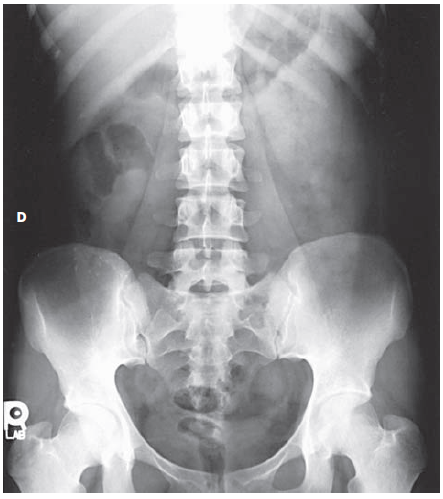
\includegraphics[width=0.7\linewidth]{imagenes/abd3}
	\caption{De cúpulas diafragmáticas hacia abajo}
	\label{fig:abd3}
\end{figure}


\clearpage
\twocolumn

%----------------------------------------------------------
%  Para agregar otro enfoque duplicá el bloque
%  desde \subsection hasta \textbf{Trucos}
%----------------------------------------------------------


%%%%%%%%%%%%%%%%%%%%%%%%%%%%%%%%%%%%%%%%%%%%%%%%%%%%%%%%%%%
%  SECCIÓN: Abdomen
%  Archivo: secciones/abdomen.tex
%  Sin preámbulo ni \begin{document} — lo maneja main.tex
	%%%%%%%%%%%%%%%%%%%%%%%%%%%%%%%%%%%%%%%%%%%%%%%%%%%%%%%%%%%
	
	\section{Abdomen}
	
	\subsection{AP Decúbito Lateral Izquierdo --- RC Horizontal (Frente Lateralizado)}
	
	\subsubsection*{1. Identificación}
	
	\textbf{Tipo:} Proyección complementaria. Suplanta la proyección frente en bipedestación cuando el paciente no puede ponerse de pie.
	
	\textbf{Indicaciones clínicas principales:}
	\begin{itemize}
		\item Sospecha de neumoperitoneo (aire libre intraperitoneal)
		\item Detección de niveles hidroaéreos en paciente sin tolerancia a la bipedestación
		\item Paciente en estado crítico o con movilidad muy reducida
	\end{itemize}
	
	\subsubsection*{2. Técnica Base}
	
	\textbf{Receptor de imagen:} 35$\times$43 cm. Orientación \textbf{transversal}, siguiendo el eje longitudinal de la región abdominal.
	
	\textbf{DFRI:} 100 cm. Distancia estándar para abdomen simple.
	
	\textbf{Técnica:} Alto kVp (técnica básica). Permite visualizar el aire libre como zona radiolúcida sobre el fondo gris de los órganos sólidos; el RC atraviesa el abdomen de forma horizontal para que el aire, al ascender por flotabilidad, quede proyectado en el margen superior de la cavidad.
	
	\textbf{Factores técnicos:} kVp \textbf{[dato no suministrado]} --- mAs \textbf{[dato no suministrado]}. Espesor medido a nivel de las crestas ilíacas.
	
	\textbf{Bucky:} Bucky de mesa con grilla.
	
	\subsubsection*{3. Posicionamiento}
	
	\paragraph{Paciente}
	Decúbito lateral izquierdo (perfil), apoyando el flanco izquierdo sobre la mesa o camilla. Se prefiere el lado izquierdo para evitar que el aire libre se confunda con la burbuja gástrica, que normalmente ocupa ese hemiabdomen. Si es posible, mantener al paciente en esta posición durante al menos 5 minutos antes de la exposición para permitir que el aire libre ascienda a su máxima altura y el líquido intraperitoneal se redistribuya hacia el flanco izquierdo.
	
	\begin{figure}[h]
		\centering
		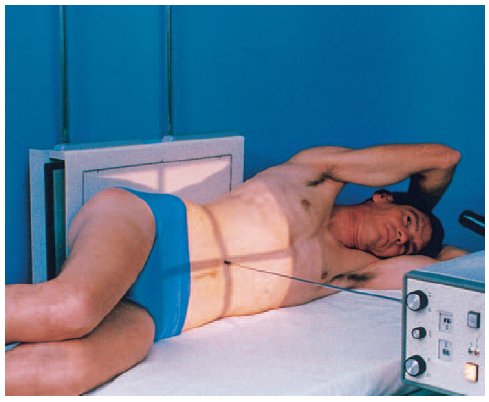
\includegraphics[width=0.7\linewidth]{imagenes/abd5}
		\caption{}
		\label{fig:abd5}
	\end{figure}
	
	
	\paragraph{Región de interés}
	Crestas ilíacas centradas sobre el receptor de imagen. Rodillas parcialmente flexionadas, apoyadas una sobre la otra, para estabilizar al paciente. Brazos elevados por encima del nivel del diafragma y apoyados bajo la cabeza, de modo que no se superpongan sobre el contenido abdominal.
	
	\paragraph{Rayo Central}
	Horizontal, perpendicular al plano del receptor. Punto de entrada: \textbf{centro de la región abdominal, 5 cm por encima de las crestas ilíacas}.
	
	\paragraph{Receptor de imagen}
	Centrado a nivel de las crestas ilíacas. Debe incluir ambos diafragmas en el margen superior y la sínfisis del pubis en el margen inferior. El receptor se coloca vertical, paralelo al eje longitudinal del paciente.
	
	\paragraph{Respiración}
	Al final de la espiración. Reduce el volumen pulmonar y desciende los diafragmas, ampliando el espacio visible de la cavidad abdominal superior. Si el paciente está lúcido, solicitarle colaboración activa para sostener la apnea.
	
	\subsubsection*{4. Anatomía Visible}
	
	Cavidad abdominal completa con ambos diafragmas incluidos. Silueta hepática en el hemiabdomen derecho. Burbuja gástrica en el hemiabdomen izquierdo. Niveles hidroaéreos dentro de las asas intestinales. Aire libre intraperitoneal proyectado sobre la silueta del hígado (lado derecho, margen superior) cuando existe neumoperitoneo. El lado superior es el de mayor relevancia diagnóstica para detección de aire libre.
	
	\subsubsection*{5. Criterios de Evaluación}
	
	\textbf{Posicionamiento correcto:} Ambos diafragmas incluidos en el campo. RC horizontal confirmado por la visualización de niveles líquidos perfectamente horizontales dentro de las asas. Crestas ilíacas centradas en la imagen.
	
	\textbf{Ausencia de rotación:} Alas ilíacas simétricas. Bordes costales inferiores externos equidistantes respecto a la columna vertebral. Cuerpos vertebrales sin oblicuidad apreciable.
	
	\textbf{Penetración y contraste:} Escala de grises que permite distinguir el aire libre (negro) sobre el fondo gris de los órganos sólidos. Niveles hidroaéreos visibles tanto en posición superior (gas) como inferior (líquido) dentro de las asas intestinales. Aire intraperitoneal libre identificable sobre la silueta hepática.
	
	\subsubsection*{6. Puntos Críticos}
	
	\textbf{RC no horizontal:} Si el RC no es estrictamente horizontal, los niveles hidroaéreos se distorsionan y el aire libre puede no proyectarse en el margen correcto, llevando a falsos negativos. Verificar la horizontalidad del tubo antes de exponer.
	
	\textbf{Tiempo insuficiente en decúbito:} Si no se respetan los 5 minutos previos, el aire libre puede no haber ascendido lo suficiente y quedar oculto. Cuando la situación clínica lo permita, respetar el tiempo de espera.
	
	\textbf En pacientes con trauma abdominal severo o inestabilidad hemodinámica, la exposición se realiza con el mínimo movimiento posible; se puede posicionar el receptor sin mover al paciente del transporte si la situación lo requiere.
	
	\textbf{Trucos:} Visualizar siempre el lado superior de la imagen al evaluar: es donde se proyecta el aire libre. La burbuja gástrica en el lado izquierdo no debe confundirse con neumoperitoneo; el decúbito izquierdo aleja precisamente ese artefacto del área diagnóstica crítica (margen hepático derecho).
	
	\onecolumn
	
	\begin{figure}
		\centering
		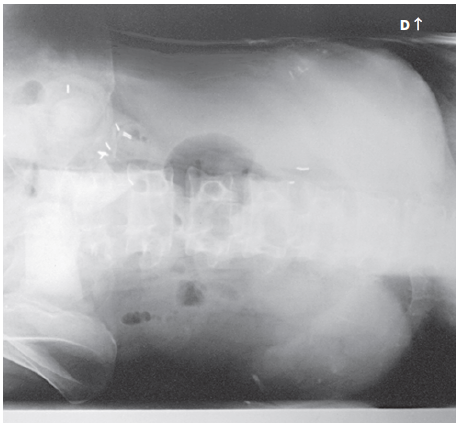
\includegraphics[width=0.7\linewidth]{imagenes/abd6}
		\caption{}
		\label{fig:abd6}
	\end{figure}
	
	\twocolumn

\clearpage

	
	%----------------------------------------------------------
	%  Para agregar otro enfoque duplicá el bloque
	%  desde \subsection hasta \textbf{Trucos}
	%----------------------------------------------------------
	
	
%%%%%%%%%%%%%%%%%%%%%%%%%%%%%%%%%%%%%%%%%%%%%%%%%%%%%%%%%%%
%  SECCIÓN: Abdomen
%  Archivo: secciones/abdomen.tex
%  Sin preámbulo ni \begin{document} — lo maneja main.tex
	%%%%%%%%%%%%%%%%%%%%%%%%%%%%%%%%%%%%%%%%%%%%%%%%%%%%%%%%%%%
	
	\section{Abdomen}
	
	\subsection{Abdomen Perfil}
	
	\subsubsection*{1. Identificación}
	
	\textbf{Tipo:} Proyección complementaria. Forma par con la proyección frente de abdomen.
	
	\textbf{Indicaciones clínicas principales:}
	\begin{itemize}
		\item Localización tridimensional de cuerpo extraño
		\item Aneurisma o calcificación de aorta abdominal
		\item Neoplasias, ascitis y exploraciones con medio de contraste
	\end{itemize}
	
	\subsubsection*{2. Técnica Base}
	
	\textbf{Receptor de imagen:} 35 $\times$ 43 cm. Orientación \textbf{longitudinal} en relación con el eje mayor de la región.
	
	\textbf{DFRI:} 100 cm. Distancia estándar para estudios de abdomen.
	
	\textbf{Técnica:} Básica o contrastada según indicación. A mayor espesor, mayor kVp requerido.
	
	\textbf{Factores técnicos:} kVp \textbf{[dato no suministrado]} --- mAs \textbf{[dato no suministrado]}. Medir el espesor en la región de mayor grosor abdominal.
	
	\textbf{Bucky:} Bucky mural (bipedestación) o Bucky de mesa (decúbito lateral). Con grilla.
	
	\subsubsection*{3. Posicionamiento}
	
	\paragraph{Paciente}
	De pie (bipedestación) o en decúbito lateral derecho o izquierdo. Plano medio sagital paralelo al receptor. Codos flexionados con ambos brazos levantados por encima de la cabeza, alejándose de la región abdominal.
	
	\begin{figure}[h]
		\centering
		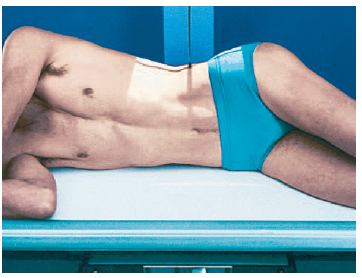
\includegraphics[width=0.7\linewidth]{imagenes/abd7}
		\caption{}
		\label{fig:abd7}
	\end{figure}
	
	
	\paragraph{Región de interés}
	Pelvis sin rotación. Rodillas flexionadas para reducir la lordosis lumbar; colocar apoyo bajo rodillas y tobillos en decúbito. Plano coronal del paciente perpendicular al receptor.
	
	\paragraph{Rayo Central}
	Perpendicular al plano del receptor. Punto de entrada: \textbf{5 cm por encima de las crestas ilíacas, al plano medio coronal}, de modo que incluya el diafragma.
	
	\paragraph{Receptor de imagen}
	Centrado a la altura de las crestas ilíacas (o 5 cm por encima). Debe incluir desde las cúpulas diafragmáticas hasta la pelvis, y los bordes anterior y posterior del abdomen.
	
	\paragraph{Respiración}
	Al final de la espiración. Permite mayor inclusión del diafragma y reduce la superposición de estructuras intestinales.
	
	\subsubsection*{4. Anatomía Visible}
	
	Asas intestinales, niveles hidroaéreos si presentes, aorta abdominal y sus calcificaciones, columna lumbar en perfil, cúpulas diafragmáticas, retroperitoneo y pelvis ósea. La columna debe verse recta y alineada con el receptor. Los huesos ilíacos deben aparecer superpuestos (con magnificación inevitable de uno respecto al otro por la divergencia del haz). No se incluye la sínfisis del pubis.
	
	\subsubsection*{5. Criterios de Evaluación}
	
	\textbf{Posicionamiento correcto:} Abdomen de perfil visible desde cúpulas diafragmáticas hasta pelvis; columna lumbar alineada con el receptor; sínfisis del pubis excluida.
	
	\textbf{Ausencia de rotación:} Bordes posteriores de los arcos costales superpuestos; bordes posteriores de las alas ilíacas superpuestos. Un ilíaco siempre presentará mayor magnificación que el otro por efecto geométrico.
	
	\textbf{Penetración y contraste:} Asas intestinales y niveles hidroaéreos diferenciables; tejidos blandos abdominales visibles en la región anterior y posterior.
	
	\subsubsection*{6. Puntos Críticos}
	
	\textbf{Rotación del paciente:} Produce asimetría de los arcos costales e ilíacos posteriores, impidiendo la localización tridimensional. Corregir alineando el plano coronal estrictamente perpendicular al receptor.
	
	\textbf{Centrado incorrecto del RC:} Si el RC se dirige a la altura exacta de crestas sin compensar, el diafragma puede quedar excluido. Subir 5 cm por encima de las crestas para asegurar su inclusión.
	
	\textbf{Adaptaciones:} En paciente politraumatizado que no puede moverse se utiliza el perfil tangencial (ver siguiente subsección). No se emplea esta proyección para diagnóstico de oclusión intestinal; en ese caso usar frente en decúbito dorsal más frente de pie.
	
	\textbf{Trucos:} Usar el cátodo en la parte superior del abdomen (región más gruesa) para obtener exposición uniforme aprovechando el efecto anódico. Colocar apoyo bajo rodillas y tobillos en decúbito lateral para mantener el plano coronal perpendicular y evitar rotación involuntaria.
	
	\clearpage
	\onecolumn
	
	\begin{figure}
		\centering
		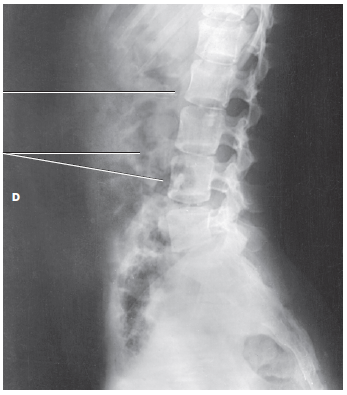
\includegraphics[width=0.7\linewidth]{imagenes/abd8}
		\caption{}
		\label{fig:abd8}
	\end{figure}
	
	
	
	\twocolumn
	\clearpage	
	%----------------------------------------------------------
	
	\subsection{Abdomen Perfil Tangencial}
	
	\subsubsection*{1. Identificación}
	
	\textbf{Tipo:} Proyección complementaria. Variante del perfil de abdomen para pacientes que no pueden adoptar bipedestación ni movilizarse.
	
	\textbf{Indicaciones clínicas principales:}
	\begin{itemize}
		\item Paciente que no puede ponerse de pie
		\item Paciente politraumatizado con imposibilidad de movimiento
		\item Sospecha de neumoperitoneo en paciente inmovilizado
	\end{itemize}
	
	\subsubsection*{2. Técnica Base}
	
	\textbf{Receptor de imagen:} 35 $\times$ 43 cm. Orientación \textbf{longitudinal} en relación con el eje mayor de la región.
	
	\textbf{DFRI:} 100 cm. Distancia estándar para estudios de abdomen.
	
	\textbf{Técnica:} Básica o contrastada según indicación.
	
	\textbf{Factores técnicos:} kVp \textbf{[dato no suministrado]} --- mAs \textbf{[dato no suministrado]}. Medir el espesor en la región de mayor grosor abdominal.
	
	\textbf{Bucky:} Con grilla. Adaptado a la posición del paciente (Bucky mural con tubo horizontal).
	
	\subsubsection*{3. Posicionamiento}
	
	\paragraph{Paciente}
	\textit Paciente decúbito supino, con brazos fuera del campo visual
	
	\begin{figure}[h]
		\centering
		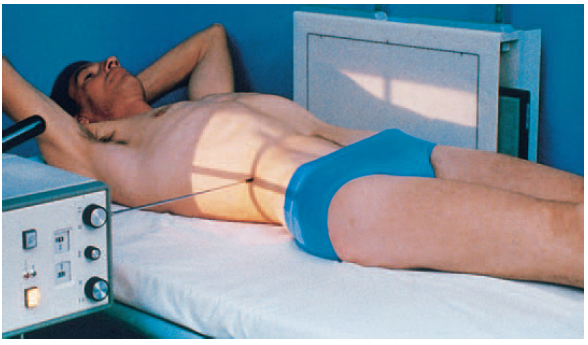
\includegraphics[width=0.7\linewidth]{imagenes/abd9}
		\caption{}
		\label{fig:abd9}
	\end{figure}
	
	\paragraph{Rayo Central}
	Perpendicular al plano del receptor, dirigido horizontalmente. Punto de entrada: \textbf{a la altura de las crestas ilíacas, al plano medio coronal}.
	
	\paragraph{Receptor de imagen}
	Centrado a la altura de las crestas ilíacas. Debe incluir desde las cúpulas diafragmáticas hasta la pelvis y los bordes anterior y posterior del abdomen.
	
	\paragraph{Respiración}
	\textit{suspendida en al final de una experiacion}
	
	\subsubsection*{4. Anatomía Visible}
	
	Abdomen de perfil desde cúpulas diafragmáticas hasta pelvis. Huesos ilíacos superpuestos como indicador de ausencia de rotación. En caso de neumoperitoneo, el aire libre se visualiza en la región anterior del abdomen (entre la pared abdominal anterior y el hígado/vísceras).
	
	\subsubsection*{5. Criterios de Evaluación}
	
	\textbf{Posicionamiento correcto:} Abdomen de perfil visible desde cúpulas diafragmáticas hasta pelvis.
	
	\textbf{Ausencia de rotación:} Huesos ilíacos superpuestos.
	
	\textbf{Penetración y contraste:} Diferenciación de tejidos blandos; región anterior del abdomen visible para detectar aire libre subdiafragmático anterior.
	
	\subsubsection*{6. Puntos Críticos}
	
	\textbf{Indicación incorrecta:} El perfil tangencial no reemplaza al perfil estándar en pacientes móviles; se reserva exclusivamente para politraumatizados o pacientes que no pueden moverse.
	
	\textbf{Rotación del paciente:} Impide la superposición de los ilíacos y dificulta la identificación de neumoperitoneo. Verificar alineación antes de la exposición.
	
	\textbf{Adaptaciones:} Técnica diseñada específicamente para pacientes con movilidad reducida o nula. El tubo se orienta horizontalmente con el receptor vertical junto al paciente.
	
	\textbf{Trucos:} La presencia de aire libre anterior al abdomen en esta proyección es indicador sensible de neumoperitoneo en el paciente inmovilizado.
	
		\clearpage
	\onecolumn
	
	\begin{figure}
		\centering
		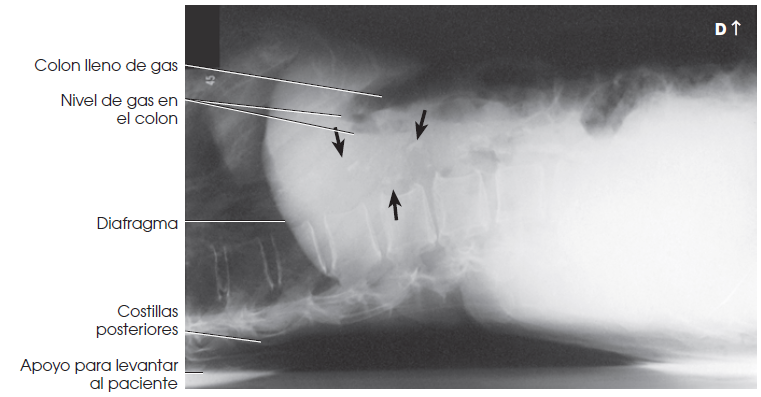
\includegraphics[width=0.7\linewidth]{imagenes/abd10}
		\caption{}
		\label{fig:abd8}
	\end{figure}
	
	
	
	\twocolumn
	\clearpage	
	%----------
	
	%----------------------------------------------------------
	%  Para agregar otro enfoque duplicá el bloque
	%  desde \subsection hasta \textbf{Trucos}
	%----------------------------------------------------------
	
	
%%%%%%%%%%%%%%%%%%%%%%%%%%%%%%%%%%%%%%%%%%%%%%%%%%%%%%%%%%%
%  SECCIÓN: Abdomen — Paciente Pediátrico
%  Archivo: secciones/abdomen_pediatrico.tex
%  Sin preámbulo ni \begin{document} — lo maneja main.tex
	%%%%%%%%%%%%%%%%%%%%%%%%%%%%%%%%%%%%%%%%%%%%%%%%%%%%%%%%%%%
	
	\section{Abdomen — Paciente Pediátrico}
	
	\subsection*{Consideraciones Clínicas}
	
	\textbf{Selección del estudio según diagnóstico clínico (DC):}
	El DC condiciona tanto la proyección como la posición del paciente. Dos situaciones frecuentes requieren criterio específico:
	
	\begin{itemize}
		\item \textbf{Abdomen agudo:} proyección de pie, incluyendo desde la sínfisis púbica hasta el diafragma.
		\item \textbf{Cuerpo extraño (CE):} frente y perfil de pie. Puede requerir campo desde peñascos hasta sínfisis púbica según tiempo de ingesta.
	\end{itemize}
	
	\textbf{Paciente que no puede estar de pie:} se realiza sentado o en decúbito lateral con RC horizontal, siempre que se requiera evaluar niveles hidroaéreos.
	
	\textbf{CE en decúbito supino:} aceptable en frente y perfil cuando no es posible la bipedestación ni la sedestación.
	
	\textbf{Protección gonadal:} aplicar siempre que no interfiera con el área de interés. En pacientes pediátricos se prioriza obtener una exposición diagnóstica correcta sin protección antes que intentar colocarla y comprometer la región de interés.
	
	\textbf{Campo de imagen:} toda la región de interés debe entrar en un único chasis.
	
	\medskip
	
	\textbf{¿Por qué de pie o sentado en CE?} Permite evaluar si el objeto puede haber perforado una víscera y determinar su localización exacta mediante niveles.
	
	\textbf{¿Por qué incluir desde peñascos hacia abajo?} Si la ingesta es reciente (menos de 2 horas), el CE puede no haber descendido al tracto digestivo y encontrarse aún en cuello o región torácica superior.
	
	\medskip
	
	\textbf{Interrogatorio previo:} preguntar a los padres o al niño (si puede comunicarse) el tiempo transcurrido desde la ingesta. Este dato orienta el nivel de búsqueda:
	
	\begin{itemize}
		\item \textbf{Menos de 2 hs:} cuello y región comprendida entre faringe y carina (vía aérea superior y esófago proximal). Se pide Rx de cuello, tórax y abdomen.
		\item \textbf{Primeras 12 hs:} estómago (tórax con porción superior de abdomen).
		\item \textbf{Más de 12 hs:} intestino delgado.
		\item \textbf{Entre 12 y 24 hs:} intestino grueso.
		\item \textbf{Más de 24 hs:} si no se visualiza, probable expulsión o localización en recto inminente.
	\end{itemize}
	
	%----------------------------------------------------------
	%  Continuar con \subsection{} para cada enfoque
	%----------------------------------------------------------
	
\clearpage
%%%%%%%%%%%%%%%%%%%%%%%%%%%%%%%%%%%%%%%%%%%%%%%%%%%%%%%%%%%
%  SECCIÓN: Aparato Urinario
%  Archivo: secciones/aparato_urinario.tex
%  Sin preámbulo ni \begin{document} — lo maneja main.tex
	%%%%%%%%%%%%%%%%%%%%%%%%%%%%%%%%%%%%%%%%%%%%%%%%%%%%%%%%%%%
	
	\section{Abdomen}
	
	\subsection{Aparato Urinario Simple (AUS) --- Proyección AP}
	
	\subsubsection*{1. Identificación}
	
	\textbf{Tipo:} Proyección básica. Radiografía exploratoria sin contraste, equivalente a un frente de abdomen. Constituye la proyección preliminar obligatoria antes de estudios con medio de contraste (UIV, uretrocistografía, etc.).
	
	\textbf{Indicaciones clínicas principales:}
	\begin{itemize}
		\item Litiasis renal o ureteral: detección de cálculos por su densidad cálcica pura (el contraste los encubriría)
		\item Valoración de calcificaciones anómalas en la vía urinaria
		\item Estudio preliminar previo a la administración de medio de contraste para identificar signos basales (obstrucción, hidronefrosis, tumores, infecciones)
	\end{itemize}
	
	\subsubsection*{2. Técnica Base}
	
	\textbf{Receptor de imagen:} 35$\times$43 cm. Orientación \textbf{longitudinal} para incluir desde T12 hasta la sínfisis del pubis. En pacientes muy altos, se realiza una primera exposición con este chasis y se complementa con un segundo receptor de 24$\times$30 cm en orientación \textbf{transversal}, centrado 5--7 cm por encima del borde superior de la sínfisis del pubis, para incluir la vejiga.
	
	\textbf{DFRI:} 100 cm. Distancia estándar para radiografía de abdomen.
	
	\textbf{Técnica:} Técnica intermedia. Las densidades del abdomen son muy homogéneas (bajo contraste intrínseco), por lo que se requiere una escala larga de grises para diferenciar el contorno de las vísceras (riñones), tejido adiposo, aire y estructuras óseas.
	
	\textbf{Factores técnicos:} Medición del espesor a nivel de las crestas ilíacas (L4).
	
	\textbf{Bucky:} Bucky de mesa con grilla.
	
	\subsubsection*{3. Posicionamiento}
	
	\paragraph{Paciente}
	Decúbito supino sobre la mesa de examen. El plano medio sagital (PMS) perpendicular a la mesa y centrado sobre la línea media del receptor. Los brazos colocados de manera que no proyecten sombras sobre el receptor de imagen.
	
	\begin{figure}[h]
		\centering
		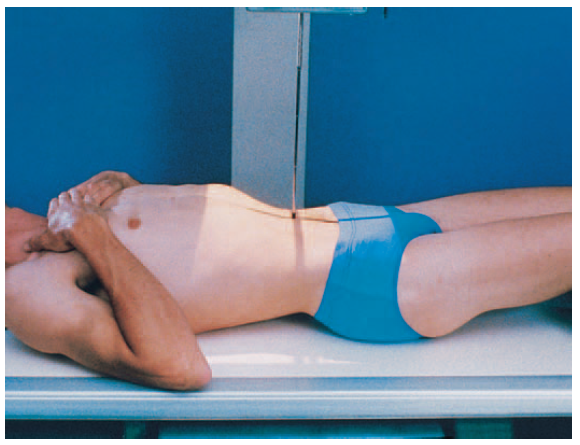
\includegraphics[width=0.7\linewidth]{imagenes/aus1}
		\caption{}
		\label{fig:aus1}
	\end{figure}
	
	
	\paragraph{Región de interés}
	Sin rotación de pelvis ni tronco: las espinas ilíacas anterosuperiores (EIAS) deben quedar equidistantes a la mesa. Leve flexión de rodillas con apoyo para aliviar la tensión lumbar. La región a incluir comprende desde T12 (polo superior de los riñones) hasta la sínfisis del pubis (incluida la vejiga, que puede extenderse por debajo de la sínfisis cuando está llena).
	
	\paragraph{Rayo Central}
	Perpendicular al plano del receptor. Punto de entrada: \textbf{a la altura de las crestas ilíacas (L4), sobre el plano medio coronal}.
	
	\paragraph{Receptor de imagen}
	Centrado a la altura de las crestas ilíacas. Borde superior en T12 para incluir los polos superiores renales; borde inferior en la sínfisis del pubis para incluir vejiga completa. En el enfoque complementario de vejiga: receptor de 24$\times$30 cm centrado 5--7 cm por encima del borde superior de la sínfisis del pubis.
	
	\paragraph{Respiración}
	Espiración máxima, suspendida. La espiración desciende el diafragma y reduce la superposición de estructuras torácicas basales sobre los riñones; la apnea elimina el movimiento de las vísceras abdominales durante la exposición.
	
	\subsubsection*{4. Anatomía Visible}
	
	Silueta completa de ambos riñones (polos superiores a nivel de T12, inferiores aproximadamente en L3--L4). Columna vertebral lumbar centrada en la imagen. Contornos de los músculos psoas. Sínfisis del pubis y vejiga urinaria. Alas ilíacas simétricas. En presencia de litiasis: opacidades cálcicas a lo largo del trayecto ureteral (desde pelvis renal hasta vejiga) o en el parénquima renal.
	
	\subsubsection*{5. Criterios de Evaluación}
	
	\textbf{Posicionamiento correcto:} Columna vertebral centrada en la radiografía. Inclusión completa desde T12 hasta la sínfisis del pubis. Silueta renal bilateral visible. Vejiga incluida en el campo.
	
	\textbf{Ausencia de rotación:} Alas ilíacas simétricas. EIAS equidistantes al eje vertical de la imagen. Apófisis espinosas centradas respecto a los pedículos vertebrales.
	
	\textbf{Penetración y contraste:} Escala larga de grises que permita diferenciar el contorno renal del tejido adiposo perirrenal, el gas intestinal y las estructuras óseas. Ausencia de artefactos por ropa interior u objetos metálicos del paciente.
	
	\subsubsection*{6. Puntos Críticos}
	
	\textbf{Paciente demasiado alto para un solo chasis:} La vejiga y la sínfisis del pubis quedan fuera del campo. Corrección: realizar primero la exposición de abdomen completo y luego un enfoque complementario de vejiga con receptor de 24$\times$30 cm transversal, centrado 5--7 cm por encima del borde superior de la sínfisis del pubis.
	
	\textbf{Rotación de pelvis o tronco:} Proyección asimétrica de las alas ilíacas y falsa lateralización de estructuras urinarias, dificultando la localización de cálculos. Corrección: verificar que las EIAS sean equidistantes a la mesa antes de disparar.
	
	\textbf{Adaptaciones:} En paciente con dificultad para el decúbito supino, puede realizarse en bipedestación (AP de pie); en ese caso verificar que no haya desplazamiento renal por efecto gravitacional que altere la región incluida.
	
	\textbf{Trucos:} Solicitar al paciente que retire ropa interior con elementos metálicos (hebillas, ganchos) para evitar artefactos sobre la región pelviana. Recordar que los cálculos NO se ven con medio de contraste: esta proyección es la única que los muestra por su densidad cálcica pura. No es indispensable incluir las cúpulas diafragmáticas; la región crítica es el polo inferior, la vejiga y la sínfisis.
	
	\begin{figure}[h]
		\centering
		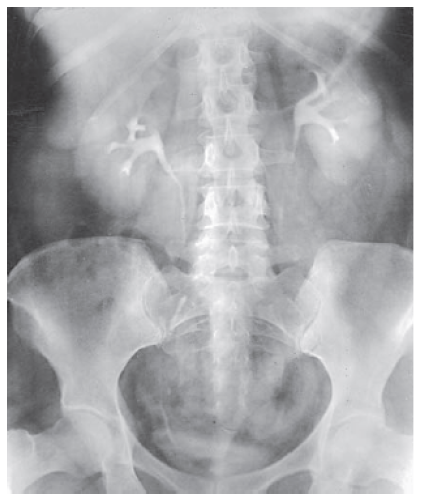
\includegraphics[width=0.7\linewidth]{imagenes/aus3}
		\caption{}
		\label{fig:aus3}
	\end{figure}
	
	\textbf{Caso:} Pct. rotado, afecta el valor diagnóstico (volver a repetirse, porque se evalúa morfología y función, si un lado está más inclinado es posible que el MC llegue mas rapido por eso mismo, falseando así el resultado).
	
	
	\clearpage
	\onecolumn
	
	\begin{figure}
		\centering
		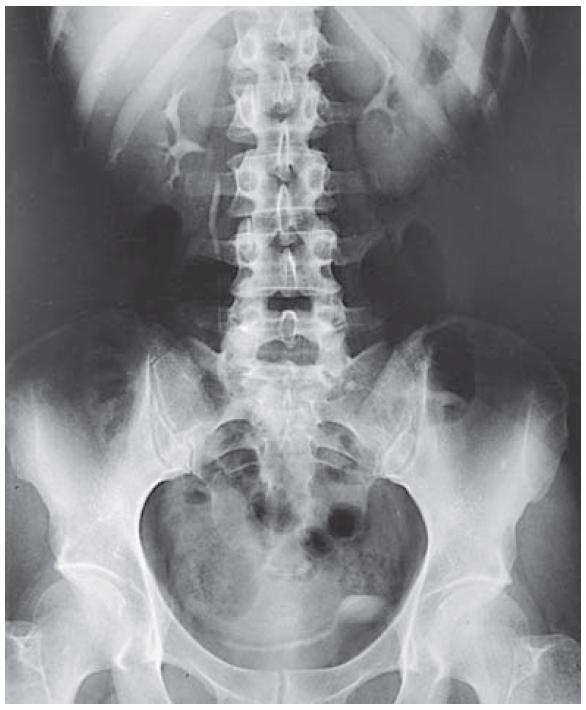
\includegraphics[width=0.7\linewidth]{imagenes/aus2}
		\caption{}
		\label{fig:aus2}
	\end{figure}
	
	
	
	\clearpage
	\twocolumn
	%----------------------------------------------------------
	%  Para agregar otro enfoque duplicá el bloque
	%  desde \subsection hasta \textbf{Trucos}
	%----------------------------------------------------------
	
	
%%%%%%%%%%%%%%%%%%%%%%%%%%%%%%%%%%%%%%%%%%%%%%%%%%%%%%%%%%%
%  SECCIÓN: Vejiga Urinaria
%  Archivo: secciones/vejiga.tex
%  Sin preámbulo ni \begin{document} — lo maneja main.tex
	%%%%%%%%%%%%%%%%%%%%%%%%%%%%%%%%%%%%%%%%%%%%%%%%%%%%%%%%%%%
	
	\section{Abdomen}
	
	\subsection{Vejiga Urinaria - Proyección AP Axial}
	
	\subsubsection*{1. Identificación}
	
	\textbf{Tipo:} Proyección complementaria. Se realiza como complemento cuando el chasis 35$\times$43 no alcanza para incluir la vejiga, o para valorar específicamente la vejiga.
	
	\textbf{Indicaciones clínicas principales:}
	\begin{itemize}
		\item Divertículo vesical
		\item Reflujo vesicoureteral
		\item Evaluación de próstata en hombres
	\end{itemize}
	
	\subsubsection*{2. Técnica Base}
	
	\textbf{Receptor de imagen:} 24$\times$30 cm. Orientación \textbf{transversal} en todos los biotipos.
	
	\textbf{DFRI:} 100 cm. Distancia estándar para estudios de pelvis con técnica convencional.
	
	\textbf{Técnica:} Intermedia. Permite diferenciar la densidad de la vejiga llena con medio de contraste respecto a las estructuras óseas (pelvis y sacro) que se encuentran por detrás.

	
	\textbf{Bucky:} Bucky de mesa con grilla.
	
	\subsubsection*{3. Posicionamiento}
	
	\paragraph{Paciente}
	Decúbito supino sobre la mesa (también puede realizarse en bipedestación). Plano medio sagital perpendicular al receptor. Brazos ubicados de modo que no proyecten sombra sobre el receptor de imagen.
	
	\begin{figure}[h]
		\centering
		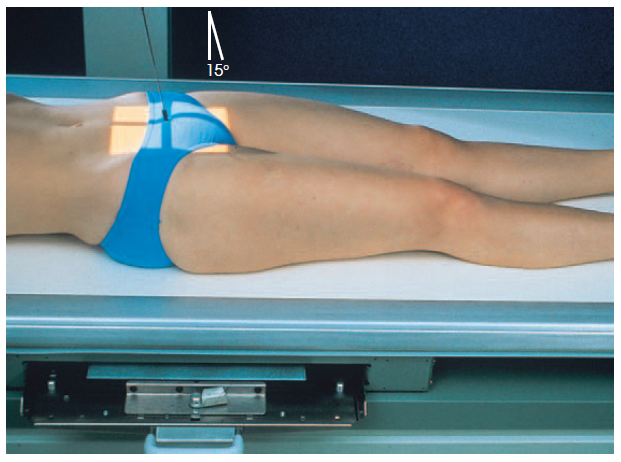
\includegraphics[width=0.7\linewidth]{imagenes/aus4}
		\caption{}
		\label{fig:aus4}
	\end{figure}
	
	
	\paragraph{Región de interés}
	Pelvis sin rotación: las espinas ilíacas anterosuperiors (EIAS) equidistantes al receptor. Piernas extendidas para lograr que la zona lumbosacra se arquee e incline hacia abajo los huesos pélvicos anteriores. Hombros en un mismo plano.
	
	\paragraph{Rayo Central}
	Angulado 10--15° en sentido caudal respecto al plano del receptor. La angulación exacta depende del grado de lordosis lumbar: a mayor lordosis, menor angulación requerida. Punto de entrada: \textbf{5 cm por encima del borde superior de la sínfisis del pubis}.
	
	\paragraph{Receptor de imagen}
	Centrado 5 cm por encima del borde superior de la sínfisis del pubis (referencia de altura equivalente al trocánter mayor del fémur). Debe incluir los extremos distales de los uréteres, la vejiga y la parte proximal de la uretra.
	
	\paragraph{Respiración}
	Espiración máxima, luego suspendida. Reduce el contenido abdominal sobre la región de interés y mejora la visualización de la vejiga.
	
	\subsubsection*{4. Anatomía Visible}
	
	Extremos distales de los uréteres (unión ureterovesical), vejiga urinaria con medio de contraste, y parte proximal de la uretra. Los huesos del pubis deben proyectarse por debajo del cuello vesical y la uretra proximal, sin superponerse a estas estructuras. La angulación caudal del RC desplaza la sínfisis del pubis hacia caudal, dejando libre la región del cuello vesical.
	
	\subsubsection*{5. Criterios de Evaluación}
	
	\textbf{Posicionamiento correcto:} La sínfisis del pubis aparece proyectada por debajo de la vejiga, sin superponer el cuello vesical ni la zona de los uréteres distales. El medio de contraste se visualiza claramente en vejiga, uréteres distales y uretra proximal.
	
	\textbf{Ausencia de rotación:} Las EIAS equidistantes respecto a la línea media; pelvis simétrica en la imagen.
	
	\textbf{Penetración y contraste:} Escala de contraste corta (alta densidad relativa) que permita diferenciar claramente el medio de contraste en la vejiga respecto a las estructuras óseas de la pelvis y el sacro subyacente.
	
	\subsubsection*{6. Puntos Críticos}
	
	\textbf{Angulación insuficiente del RC:} La sínfisis del pubis se superpone al cuello vesical y a los uréteres distales, impidiendo su evaluación. Aumentar la angulación caudal dentro del rango 10--15°.
	
	\textbf{Piernas no extendidas:} La zona lumbosacra no se arquea correctamente y los huesos pélvicos anteriores no se inclinan hacia abajo, reduciendo la efectividad de la angulación. Verificar que las piernas estén en extensión completa antes de exponer.
	
	\textbf{Adaptaciones:} En pacientes con mayor lordosis lumbar puede requerirse menor angulación (incluso por debajo de 10°). En bipedestación, verificar que el plano medio sagital se mantenga perpendicular al receptor.
	
	\textbf{Trucos:} El trocánter mayor del fémur sirve como referencia de altura para centrar el RI cuando no se palpa con facilidad el borde superior de la sínfisis. La angulación caudal es el elemento diferenciador de esta proyección respecto a la AP estándar de pelvis.
	
	
	\clearpage
	\onecolumn
	\begin{figure}
		\centering
		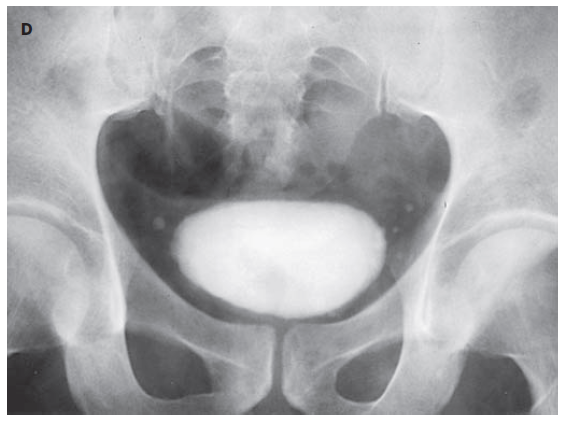
\includegraphics[width=0.7\linewidth]{imagenes/aus5}
		\caption{}
		\label{fig:aus5}
	\end{figure}
	
	\twocolumn
	\clearpage
	
	
	
	%----------------------------------------------------------
	%  Para agregar otro enfoque duplicá el bloque
	%  desde \subsection hasta \textbf{Trucos}
	%----------------------------------------------------------

%%%%%%%%%%%%%%%%%%%%%%%%%%%%%%%%%%%%%%%%%%%%%%%%%%%%%%%%%%%
%  SECCIÓN: Vejiga Urinaria
%  Archivo: secciones/vejiga.tex
%  Sin preámbulo ni \begin{document} — lo maneja main.tex
	%%%%%%%%%%%%%%%%%%%%%%%%%%%%%%%%%%%%%%%%%%%%%%%%%%%%%%%%%%%
	
	\section{Abdomen}
	
	\subsection{Vejiga - OPI/OPD}
	
	\subsubsection*{1. Identificación}
	
	\textbf{Tipo:} Proyección complementaria. Se realizan ambas oblicuas (OPD y OPI) como estudio comparativo bilateral.
	
	\textbf{Indicaciones clínicas principales:}
	\begin{itemize}
		\item Valoración de la unión ureterovesical (pasaje ureterovesical)
		\item Estudio de uréteres distales sin superposición con estructuras pélvicas
		\item Solicitud en el contexto de urografía excretora
	\end{itemize}
	
	\subsubsection*{2. Técnica Base}
	
	\textbf{Receptor de imagen:} 24$\times$30 cm. Orientación \textbf{longitudinal} (vertical).
	
	\textbf{DFRI:} 100 cm. Distancia estándar para proyecciones de abdomen y pelvis.
	
	\textbf{Técnica:} Intermedia. La rotación del paciente aumenta el espesor efectivo atravesado por el haz; se requiere mayor kVp para diferenciar la morfología interna de la vejiga sin que el medio de contraste sature la imagen.
	
	
	\textbf{Bucky:} Bucky de mesa con grilla.
	
	\subsubsection*{3. Posicionamiento}
	
	\paragraph{Paciente}
	Decúbito supino sobre la mesa de examen.
	
	\begin{figure}[h]
		\centering
		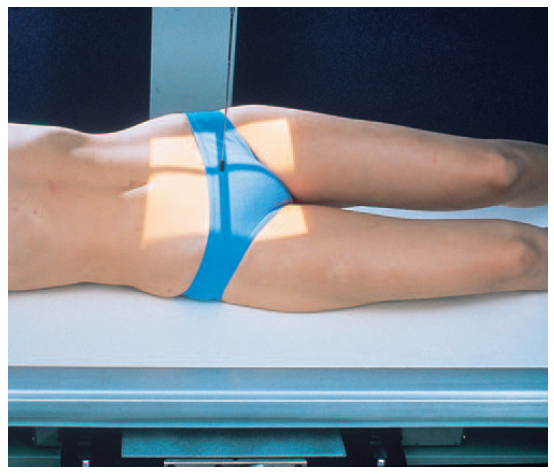
\includegraphics[width=0.7\linewidth]{imagenes/aus6}
		\caption{}
		\label{fig:aus6}
	\end{figure}
	
	
	\paragraph{Región de interés}
	Se gira al paciente 40--60° hacia el lado de interés (OPD: lado derecho apoyado; OPI: lado izquierdo apoyado). Para visualización óptima del pasaje ureterovesical, la rotación se reduce a 35°, ángulo que corresponde a la llegada del uréter a la vejiga respecto al plano coronal. La parte superior del muslo ipsilateral se extiende y abduce para evitar superposición sobre la zona vesical.
	
	\paragraph{Rayo Central}
	Perpendicular al plano del receptor. Punto de entrada: \textbf{5 cm por encima del borde superior de la sínfisis del pubis y 5 cm medial a la EIAS ipsilateral}. En estudios miccionales: perpendicular a la altura de la sínfisis púbica.
	
	\paragraph{Receptor de imagen}
	Centrado 5 cm por encima del borde superior de la sínfisis púbica y aproximadamente 5 cm medial a la EIAS (referencia Merrill: a la altura de las crestas ilíacas). Incluir los extremos distales de los uréteres, la vejiga completa y la parte proximal de la uretra.
	
	\paragraph{Respiración}
	Suspendida al final de la espiración. Estabiliza los órganos pélvicos durante la exposición.
	
	\subsubsection*{4. Anatomía Visible}
	
	Extremo distal de los uréteres, vejiga urinaria y parte proximal de la uretra. La unión ureterovesical del lado apoyado se proyecta libre de superposición. Los huesos del pubis deben proyectarse por debajo del cuello vesical y la uretra proximal. La parte superior del muslo no debe superponerse sobre la zona vesical.
	
	\subsubsection*{5. Criterios de Evaluación}
	
	\textbf{Posicionamiento correcto:} Huesos del pubis proyectados por debajo del cuello vesical y la uretra proximal. Extremos distales de los uréteres, vejiga y uretra proximal incluidos en el campo.
	
	\textbf{Ausencia de rotación:} El agujero obturador del lado apoyado aparece cerrado o estrecho; el del lado elevado aparece abierto. El ala ilíaca del lado apoyado se ve desplegada.
	
	\textbf{Penetración y contraste:} Escala de contraste semi-corta que muestre con claridad el medio de contraste en la vejiga, los uréteres distales y la uretra proximal, sin saturación de la imagen.
	
	\subsubsection*{6. Puntos Críticos}
	
	\textbf{Rotación incorrecta:} Menos de 35° superpone el uréter distal con la vejiga e impide ver el pasaje ureterovesical. Más de 60° pierde la referencia anatómica del lado de interés. Usar 35° específicamente para el pasaje ureterovesical; 40--60° para evaluación general.
	
	\textbf{Superposición del muslo:} Si no se extiende y abduce la parte superior del muslo, se cubre la región vesical inferior y la uretra proximal. Corregir la posición antes de la exposición.
	
	\textbf{Adaptaciones:} En pacientes con limitación de movilidad, usar cuñas radiolúcidas bajo el lado a elevar. En trauma pélvico, no forzar la rotación; documentar el grado alcanzado.
	
	\textbf{Trucos:} Para identificar el lado oblicuado en la radiografía: agujero obturador cerrado indica el lado hacia el que está oblicuado el paciente; agujero obturador abierto indica el lado elevado.
	
	\clearpage
	\onecolumn
	
	\begin{figure}
		\centering
		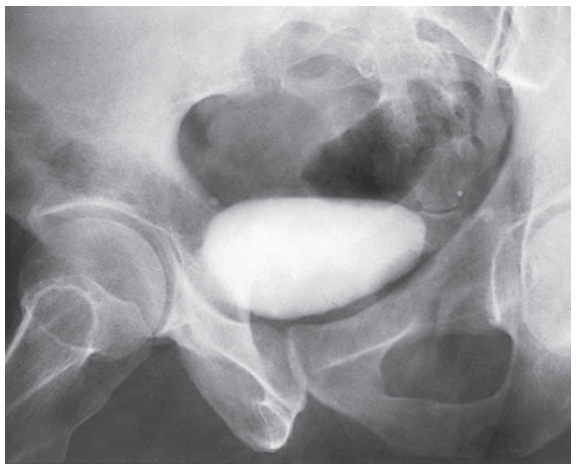
\includegraphics[width=0.7\linewidth]{imagenes/aus7}
		\caption{}
		\label{fig:aus7}
	\end{figure}
	
	\clearpage
	\twocolumn
	
	%----------------------------------------------------------
	%  Para agregar otro enfoque duplicá el bloque
	%  desde \subsection hasta \textbf{Trucos}
	%----------------------------------------------------------


%%%%%%%%%%%%%%%%%%%%%%%%%%%%%%%%%%%%%%%%%%%%%%%%%%%%%%%%%%%
%  SECCIÓN: Abdomen / Urografía
%  Archivo: secciones/abdomen.tex
%  Sin preámbulo ni \begin{document} — lo maneja main.tex
	%%%%%%%%%%%%%%%%%%%%%%%%%%%%%%%%%%%%%%%%%%%%%%%%%%%%%%%%%%%
	
	\section{Abdomen}
	
	\subsection{Urografía Intravenosa (Excretora) - OPD / OPI}
	
	\subsubsection*{1. Identificación}
	
	\textbf{Tipo:} Proyección complementaria. Forma par con la proyección AP de frente de la UIV.
	
	\textbf{Indicaciones clínicas principales:}
	\begin{itemize}
		\item Obstrucción del riñón elevado
		\item Signos de infección del tracto urinario
		\item Traumatismos en la cara inferior del uréter
	\end{itemize}
	
	\subsubsection*{2. Técnica Base}
	
	\textbf{Receptor de imagen:} 35$\times$43 cm. Orientación \textbf{longitudinal}.
	
	\textbf{DFRI:} 100 cm. Distancia estándar para estudios abdominales.
	
	\textbf{Técnica:} Intermedia o básica. \textit{[dato no suministrado sobre efecto en imagen]}.
	
	
	\textbf{Bucky:} Bucky de mesa con grilla.
	
	\subsubsection*{3. Posicionamiento}
	
	\paragraph{Paciente}
	Decúbito supino, girado de manera parcial hacia el lado derecho o izquierdo según el lado de interés. El giro permite separar el riñón elevado de la columna vertebral y proyectarlo en perfil.
	
	\begin{figure}[h]
		\centering
		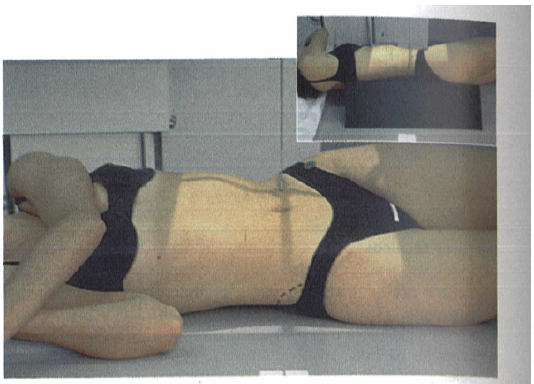
\includegraphics[width=0.7\linewidth]{imagenes/aus8}
		\caption{}
		\label{fig:aus8}
	\end{figure}
	
	
	\paragraph{Región de interés}
	Rotar el cuerpo 30° para obtener una oblicua posterior derecha (OPD) o izquierda (OPI). Flexionar la pierna del lado elevado para estabilizar el cuerpo. Elevar el brazo del lado elevado y cruzarlo sobre el tórax. Centrar la columna vertebral sobre la línea media del receptor.
	
	\paragraph{Rayo Central}
	Perpendicular al plano del receptor. Punto de entrada: \textbf{5 cm lateral a la línea media del paciente, hacia el lado elevado, a la altura de las crestas ilíacas}.
	
	\paragraph{Receptor de imagen}
	Centrado de modo que el campo incluya desde los riñones en el borde superior hasta la sínfisis del pubis en el borde inferior.
	
	\paragraph{Respiración}
	Suspendida en espiración. La espiración completa desciende el diafragma y reduce la superposición de estructuras abdominales sobre los riñones.
	
	\subsubsection*{4. Anatomía Visible}
	
	Lado elevado (alejado del RI): riñón paralelo al receptor, proyectado de frente sin superposición con la columna vertebral; uréter distal visible. Lado apoyado (próximo al RI): riñón en perfil; uréter proximal y medio proyectados lejos de la columna, despejados. Sínfisis del pubis visible en el borde inferior del campo.
	
	\subsubsection*{5. Criterios de Evaluación}
	
	\textbf{Posicionamiento correcto:} Riñón elevado paralelo al plano del receptor y separado de la columna; riñón apoyado en perfil; sínfisis del pubis incluida en el borde inferior; ambos riñones dentro del campo superior.
	
	\textbf{Ausencia de rotación:} El grado de oblicuidad es correcto cuando el riñón elevado se muestra completamente de frente sin superponerse a la columna y el riñón apoyado aparece en perfil neto.
	
	\textbf{Penetración y contraste:} \textit{[dato no suministrado]}.
	
	\subsubsection*{6. Puntos Críticos}
	
	\textbf{Oblicuidad insuficiente:} El riñón elevado se superpone a la columna vertebral, impidiendo la evaluación del uréter distal; corregir aumentando la rotación hasta 30°.
	
	\textbf{Centrado incorrecto del RC:} Desplazar el punto de entrada 5 cm hacia el lado elevado es crítico; un RC centrado en la línea media distorsiona la proyección del riñón de interés.
	
	\textbf{Adaptaciones:} En pacientes con limitación de movilidad o trauma, apoyar la oblicua con cuñas radiolúcidas para mantener los 30° de rotación sin esfuerzo del paciente.
	
	\textbf{Trucos:} Verificar antes de exponer que la columna esté centrada sobre la línea media del RI; esto asegura que el riñón elevado quede correctamente lateralizado respecto al RC.
	
	\clearpage
	\onecolumn
	
	\begin{figure}
		\centering
		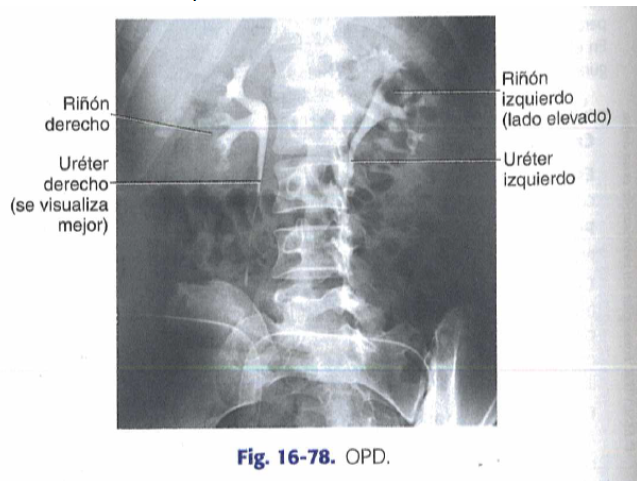
\includegraphics[width=0.7\linewidth]{imagenes/aus9}
		\caption{}
		\label{fig:aus9}
	\end{figure}
	
	\clearpage
	\twocolumn
	
	
	%----------------------------------------------------------
	%  Para agregar otro enfoque duplicá el bloque
	%  desde \subsection hasta \textbf{Trucos}
	%----------------------------------------------------------
	\input{secciones/Pelvis}
	\clearpage
\onecolumn
\thispagestyle{empty}
\vspace*{\fill}
\begin{center}
	{\color{radblue}\rule{\linewidth}{2pt}}\par
	\vspace{6mm}
	{\Huge\bfseries\color{radblue} Medición de huesos largos}\par
	\vspace{6mm}
	{\color{radblue}\rule{\linewidth}{2pt}}
\end{center}
\vspace*{\fill}
\clearpage
\twocolumn
\pagestyle{contenido}


%%%%%%%%%%%%%%%%%%%%%%%%%%%%%%%%%%%%%%%%%%%%%%%%%%%%%%%%%%%
%  SECCIÓN: Pelvis
%  Archivo: secciones/pelvis.tex
%  Sin preámbulo ni \begin{document} — lo maneja main.tex
	%%%%%%%%%%%%%%%%%%%%%%%%%%%%%%%%%%%%%%%%%%%%%%%%%%%%%%%%%%%
	
	\section{Medición de huesos largos}
	
	\subsection{Pelvimetría - AP de Pie}
	
	\subsubsection*{1. Identificación}
	
	\textbf{Tipo:} Proyección funcional. Estudio métrico de la pelvis orientado a la evaluación de ángulos y medidas estructurales del anillo pélvico.
	
	\textbf{Indicaciones clínicas principales:}
	\begin{itemize}
		\item Evaluación pré-quirúrgica o pré-obstétrica del diámetro pélvico
		\item Medición de dismetría de caderas y valoración de ángulos femorales
		\item Seguimiento de displasia del desarrollo de cadera
	\end{itemize}
	
	\subsubsection*{2. Técnica Base}
	
	\textbf{Receptor de imagen:} 35$\times$43 cm. Orientación \textbf{transversal (apaisado)}. El receptor debe ser cuadriculado especial para permitir las mediciones métricas. En ausencia del chasis cuadriculado, puede emplearse software de medición en el negatoscopio o sistema PACS.
	
	\textbf{DFRI:} 100 cm. Distancia estándar para técnica convencional de pelvis, permite reproducibilidad de las mediciones y minimiza la magnificación geométrica.
	
	\textbf{Técnica:} Intermedia, equivalente a la técnica estándar de pelvis. Permite visualizar partes blandas y estructuras óseas en equilibrio adecuado de contraste para realizar las mediciones.
	
	\textbf{Bucky:} Bucky mural con grilla. Se utiliza bucky mural ya que el paciente se posiciona de pie.
	
	\subsubsection*{3. Posicionamiento}
	
	\paragraph{Paciente}
	Paciente de pie, descalzo, de frente al receptor. La posición descalza es fundamental para evitar la influencia del calzado en la nivelación de la pelvis y garantizar la reproducibilidad de las mediciones.
	
	% TODO: \usepackage{graphicx} required
	\begin{figure}[h]
		\centering
		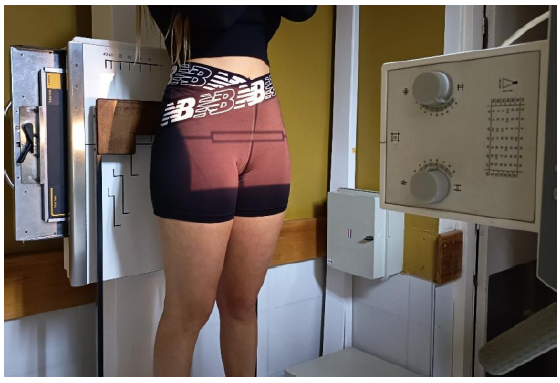
\includegraphics[width=0.7\linewidth]{imagenes/medi1}
		\caption{}
		\label{fig:medi1}
	\end{figure}
	
	
	\paragraph{Región de interés}
	Miembros inferiores con rotación interna para desplegar los cuellos femorales en toda su longitud, permitiendo su correcta valoración métrica. Esta rotación contrarrestará la anteversión femoral fisiológica.
	
	\paragraph{Rayo Central}
	Perpendicular al plano del receptor. Punto de entrada: \textbf{punto medio entre ambas espinas ilíacas anterosuperiores (EIAS)}.
	
	\paragraph{Receptor de imagen}
	Centrado al punto medio entre las EIAS. La región a incluir abarca desde las crestas ilíacas superiormente hasta la parte proximal de ambos fémures inferiormente, incluyendo la totalidad del anillo pélvico.
	
	\paragraph{Respiración}
	Respiración normal, sin apnea requerida. La región pélvica no se ve afectada por los movimientos respiratorios en un estudio en bipedestación.
	
	\subsubsection*{4. Anatomía Visible}
	
	Anillo pélvico completo con ambas alas ilíacas, sacro y cóccix. Articulaciones sacroilíacas simétricas. Cabezas femorales, cuellos femorales desplegados por la rotación interna, trocánteres mayores y menores. Articulaciones coxofemorales bilaterales. Sínfisis del pubis al centro.
	
	Las mediciones se realizan sobre el receptor cuadriculado o mediante software, trazando las siguientes referencias:
	\begin{itemize}
		\item \textbf{Línea A:} paralela a la línea de eburnación
		\item \textbf{Líneas B:} paralelas a la plomada a través de las cabezas femorales
		\item \textbf{Línea C:} perpendicular a la línea de la plomada
		\item \textbf{Valor D:} dismetría medida entre ambas cabezas femorales (Tilley, P.; 1966. Irvin, R., 1991). La dismetría puede medirse también con caliper digital en negatoscopio.
	\end{itemize}
	
	% TODO: \usepackage{graphicx} required
	\begin{figure}
		\centering
		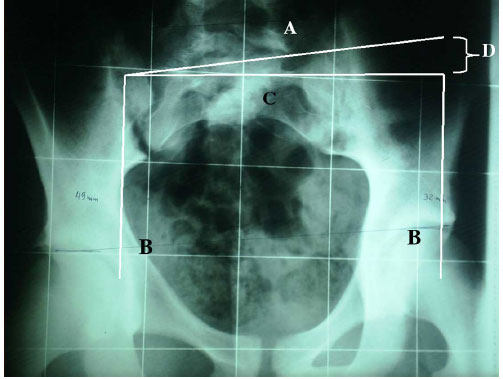
\includegraphics[width=0.7\linewidth]{imagenes/medi3}
		\caption{}
		\label{fig:medi3}
	\end{figure}
	
	
	\subsubsection*{5. Criterios de Evaluación}
	
	\textbf{Posicionamiento correcto:} Ambas espinas ilíacas anterosuperiores equidistantes del borde lateral del receptor. Cuellos femorales visibles en su totalidad sin acortamiento. Sacro proyectado en la línea media.
	
	\textbf{Ausencia de rotación:} Simetría de las alas ilíacas bilaterales. Agujeros obturadores de igual forma y tamaño a ambos lados. Articulaciones sacroilíacas simétricas.
	
	\textbf{Penetración y contraste:} Visualización simultánea de partes blandas pélvicas y estructuras óseas. Cuerpos vertebrales lumbares bajos visibles con densidad adecuada. Trabéculas del hueso esponjoso de cabezas femorales perceptibles para permitir las mediciones métricas.
	
	\subsubsection*{6. Puntos Críticos}
	
	\textbf{Calzado no retirado:} Introduce una diferencia artificial en la altura pélvica que invalida la medición de dismetría. Siempre verificar que el paciente esté descalzo antes de la exposición.
	
	\textbf{Rotación interna insuficiente de MMII:} Los cuellos femorales se proyectan acortados o superpuestos con los trocánteres mayores, imposibilitando la correcta medición del eje femoral. Corregir orientando los pies con las puntas hacia adentro.
	
	\textbf{Adaptaciones:} En pacientes con limitación de la rotación interna (prótesis, artrosis severa), documentar la posición real utilizada ya que afectará la interpretación de las mediciones. En pacientes que no pueden mantenerse de pie, consultar con el médico la viabilidad de técnica alternativa.
	
	\textbf{Trucos:} Si no se dispone del receptor cuadriculado especial, el estudio puede realizarse con receptor estándar y las mediciones se efectúan posteriormente mediante software en la estación de trabajo o PACS. La posición de pie es inherente a la naturaleza funcional del estudio, ya que reproduce la carga axial real sobre la pelvis.
	
	\onecolumn
	\clearpage
	
	% TODO: \usepackage{graphicx} required
	\begin{figure}
		\centering
		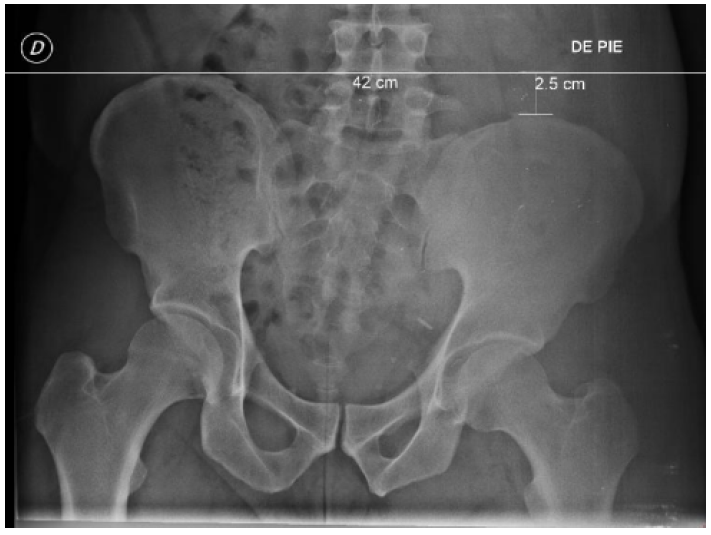
\includegraphics[width=0.7\linewidth]{imagenes/medi2}
		\caption{}
		\label{fig:medi2}
	\end{figure}
	
	\twocolumn
	\clearpage
	%----------------------------------------------------------
	%  Para agregar otro enfoque duplicá el bloque
	%  desde \subsection hasta \textbf{Trucos}
	%----------------------------------------------------------
	
%%%%%%%%%%%%%%%%%%%%%%%%%%%%%%%%%%%%%%%%%%%%%%%%%%%%%%%%%%%
%  SECCIÓN: Miembro Inferior — Medición
%  Archivo: secciones/green_ortorradiografia.tex
%  Sin preámbulo ni \begin{document} — lo maneja main.tex
	%%%%%%%%%%%%%%%%%%%%%%%%%%%%%%%%%%%%%%%%%%%%%%%%%%%%%%%%%%%
	
	\section{Medición de huesos largos}
	
	\subsection{Método de Green - Ortorradiografía (AP Bilateral Comparativa)}
	
	\subsubsection*{1. Identificación}
	
	\textbf{Tipo:} Estudio bilateral comparativo. Comprende tres enfoques secuenciales sobre el mismo receptor: articulación de la cadera, rodilla y tobillo (tibiotarsiana).
	
	\textbf{Indicaciones clínicas principales:}
	\begin{itemize}
		\item Dismetría funcional o estructural de miembros inferiores
		\item Escoliosis o desviación de columna por diferencia de longitud de miembros
		\item Control de crecimiento (hipometría o hipermetría)
	\end{itemize}
	
	\subsubsection*{2. Técnica Base}
	
	\textbf{Receptor de imagen:} 35$\times$43 cm. Orientación \textbf{apaisada (transversal)}, dividido en tres franjas de 14 cm aproximadamente, una por articulación.
	
	\textbf{DFRI:} 100 cm. Distancia estándar para este estudio; su cumplimiento estricto es condición indispensable para que las mediciones sean fidedignas.
	
	\textbf{Técnica:} Se calculan \textbf{tres técnicas independientes}, una por articulación.
	\begin{itemize}
		\item \textbf{Cadera:} técnica intermedia, ya que el RC ingresa al PMS y no está focalizado en la cadera; al ser un estudio bilateral se atraviesa más tejido y se genera mayor radiación dispersa. Esta técnica actúa como base, aportando densidad uniforme para ambas articulaciones.
		\item \textbf{Rodilla:} técnica homogeneizada respecto al disparo de cadera.
		\item \textbf{Tobillo:} técnica homogeneizada respecto al disparo de cadera.
	\end{itemize}
	El disparo de cadera permite visualizar desde la densidad alta del fémur proximal hasta las partes blandas y el trabeculado óseo a nivel distal.
	
	\textbf{Bucky:} Bucky de mesa con grilla. Se desplaza tanto el tubo de rayos como el receptor de imagen entre cada disparo.
	
	\subsubsection*{3. Posicionamiento}
	
	\paragraph{Paciente}
	Decúbito supino (proyección AP), inmovilizado durante las tres tomas. Las piernas se cinchan para mantener la posición. Se solicita al paciente que se relaje y permanezca flojo. Se le debe retirar el pantalón o subirlo lo máximo posible. Si presenta prótesis, se tracciona desde los hombros; de lo contrario, desde los pies. La comunicación constante con el paciente durante el estudio es fundamental para garantizar su colaboración y la fidelidad de las mediciones.
	
	\begin{figure}[h]
		\centering
		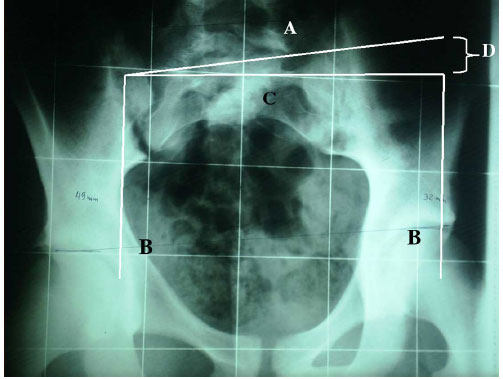
\includegraphics[width=0.7\linewidth]{imagenes/medi3}
		\caption{}
		\label{fig:medi3}
	\end{figure}
	
	
	\paragraph{Región de interés}
	Pelvis sin rotación, con las EIAS equidistantes al receptor de imagen. Miembros inferiores extendidos con rotación medial de 10--15°.
	
	\paragraph{Rayo Central}
	\begin{itemize}
		\item \textbf{Cadera:} RC perpendicular al receptor, punto de entrada 2,5 cm proximal a la sínfisis del pubis.
		\item \textbf{Rodilla:} RC perpendicular al receptor, a la altura del vértice de la rótula.
		\item \textbf{Tobillo:} RC perpendicular al receptor, a la altura de los maléolos.
	\end{itemize}
	
	\paragraph{Receptor de imagen}
	Centrado de modo que cada articulación quede incluida en su franja correspondiente del receptor. Las tres articulaciones se registran en el mismo chasis. La región a incluir comprende articulaciones de cadera, rodillas y tobillos (tibiotarsianas).
	
	\paragraph{Respiración}
	Respiración normal. No se requiere apnea. Lo determinante para la validez del estudio es la inmovilidad del paciente durante cada disparo.
	
	\subsubsection*{4. Anatomía Visible}
	
	Articulaciones de cadera bilateral, rodillas y tobillos en una sola imagen. Fémur proximal con alta densidad ósea, trabeculado y partes blandas a nivel distal. En pacientes pediátricos se visualizan las líneas de crecimiento, lo cual es un hallazgo de relevancia clínica. El estudio no presenta magnificación: es fidedigno a la estructura anatómica real, a diferencia de la telerradiografía.
	
	\subsubsection*{5. Criterios de Evaluación}
	
	\textbf{Posicionamiento correcto:} Cada articulación centrada en su franja del receptor; pelvis sin rotación con EIAS simétricas; miembros inferiores con rotación medial uniforme de 10--15°.
	
	\textbf{Ausencia de rotación:} Simetría bilateral de las articulaciones de cadera, rodillas y tobillos; fémures sin rotación visible.
	
	\textbf{Penetración y contraste:} Densidad adecuada en cadera (fémur proximal y partes blandas visibles simultáneamente); rodilla y tobillo con escala de grises homogeneizada respecto al disparo de cadera. Las tres articulaciones deben mostrar detalle trabecular.
	
	\subsubsection*{6. Puntos Críticos}
	
	\textbf{Movimiento del paciente entre disparos:} Invalida las mediciones de dismetría; el estudio deja de ser fidedigno. Corrección: inmovilizar con cinchas, explicar el procedimiento, hablarle al paciente antes de cada disparo indicándole que mantenga la posición y mirarlo constantemente durante el estudio.
	
	\textbf{Falta de protección gonadal:} Debe colocarse el protector gonadal sin que interfiera en el área de interés, especialmente en niños, donde también se deben visualizar las líneas de crecimiento.
	
	\textbf{Adaptaciones:} En pacientes con prótesis, la tracción se realiza desde los hombros en lugar de los pies. En pacientes pediátricos, verificar visibilidad de líneas de crecimiento en cada disparo.
	
	\textbf{Trucos:} Este estudio no muestra el hueso en su longitud completa, lo que impide visualizar áreas deformadas o patológicas de las diáfisis femorotibiales (limitación compensada por la telerradiografía). La diferencia de longitud entre miembros debe ser mínima para que el estudio sea concluyente. Recordar que es la colimación estrecha y el desplazamiento coordinado de tubo y receptor lo que permite los tres enfoques en un único chasis.
	
	\onecolumn
	\clearpage
	
	\begin{figure}
		\centering
		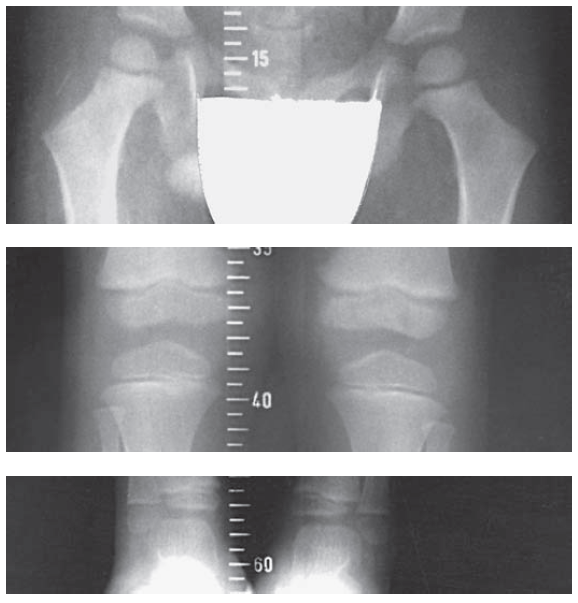
\includegraphics[width=0.7\linewidth]{imagenes/medi4}
		\caption{Una pierna}
		\label{fig:medi4}
	\end{figure}
	
	\begin{figure}
		\centering
		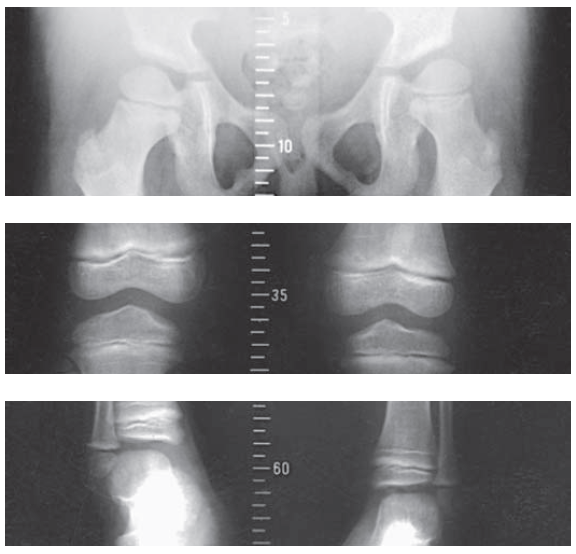
\includegraphics[width=0.7\linewidth]{imagenes/medi5}
		\caption{Ambas piernas}
		\label{fig:medi5}
	\end{figure}
	
	
	\twocolumn
	\clearpage
	%----------------------------------------------------------
	%  Para agregar otro enfoque duplicá el bloque
	%  desde \subsection hasta \textbf{Trucos}
	%----------------------------------------------------------
	
	
%%%%%%%%%%%%%%%%%%%%%%%%%%%%%%%%%%%%%%%%%%%%%%%%%%%%%%%%%%%
%  SECCIÓN: Goniometría
%  Archivo: secciones/goniometria.tex
%  Sin preámbulo ni \begin{document} — lo maneja main.tex
	%%%%%%%%%%%%%%%%%%%%%%%%%%%%%%%%%%%%%%%%%%%%%%%%%%%%%%%%%%%
	
	\section{Medición de huesos largos}
	
	\subsection{Goniometría - Telerradiografía de Miembros Inferiores}
	
	\subsubsection*{1. Identificación}
	
	\textbf{Tipo:} Estudio funcional comparativo bilateral o monopodalico. Puede realizarse de forma bilateral o monopodalica según indicación clínica.
	
	\textbf{Indicaciones clínicas principales:}
	\begin{itemize}
		\item Evaluación y medición de deformidades angulares del miembro inferior (genu varo, genu valgo)
		\item Planificación prequirúrgica en ortopedia y traumatología
		\item Seguimiento evolutivo de correcciones terapéuticas y patologías degenerativas
		\item Evaluación de secuelas post-traumáticas en medicina laboral y legal (determinación de incapacidad)
	\end{itemize}
	
	\subsubsection*{2. Técnica Base}
	
	\textbf{Receptor de imagen:} 35 $\times$ 43 cm. Orientación \textbf{vertical} en posición mural; en equipos convencionales el receptor se divide en tres sectores longitudinales de 14 cm cada uno para la técnica de tres exposiciones. En niños puede utilizarse un solo receptor según el tamaño del paciente.
	
	\textbf{DFRI:} 180 cm mínimo; óptimo a 200--250 cm. La mayor distancia reduce la magnificación inherente al estudio, aunque persiste un error aproximado del 15\% que puede paliarse con el uso de reglas radio-opacas de longitud conocida colocadas a la misma distancia que los huesos a medir.
	
	\textbf{Técnica:} Intermedia y homogenizada, adaptada a cada segmento anatómico según su grosor. Los valores de kVp se ajustan por región: cadera 75 kVp, rodilla 62 kVp, tobillo 54 kVp. Los mAs son variables y se calculan en función del grosor de la región a exponer. Al aumentar la DFRI a 2 metros se aplica compensación por ley del cuadrado inverso (factor $\times$4); técnica intermedia de referencia: 140 mAs a 2 metros.
	
	\textbf{Bucky:} Bucky mural con grilla. El paciente se posiciona con la espalda apoyada contra el bucky mural durante todo el estudio.
	
	\subsubsection*{3. Posicionamiento}
	
	\paragraph{Paciente}
	De pie, descalzo, sobre un cajón de madera elevador, con la espalda apoyada contra el bucky mural. El peso corporal debe distribuirse de forma simétrica y equitativa sobre ambos miembros. La tracción para alinear el miembro se realiza desde los miembros inferiores; en pacientes con prótesis de cadera se utiliza tracción axilar para evitar complicaciones.
	
	\begin{figure}[h]
		\centering
		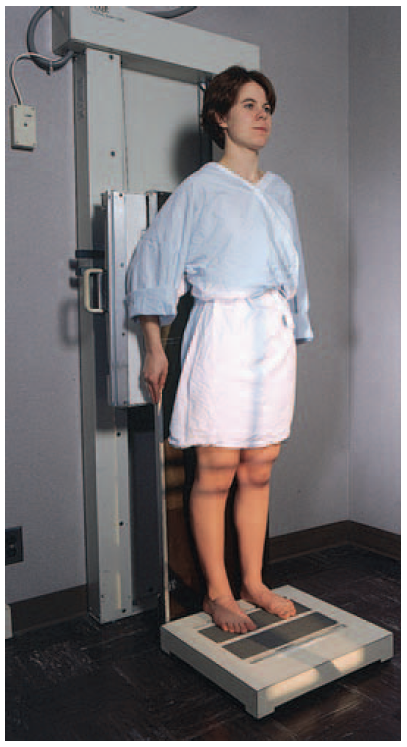
\includegraphics[width=0.7\linewidth]{imagenes/medi6}
		\caption{En esta imagen se usa un chasis propio para telerradiografia}
		\label{fig:medi6}
	\end{figure}
	
	
	\paragraph{Región de interés}
	Leve rotación interna de los miembros inferiores para desplegar el cuello femoral y estandarizar la posición. Las rótulas deben quedar orientadas al frente como referencia de ausencia de rotación. Ambos miembros deben mantenerse en posición comparable y simétrica durante todo el estudio.
	
	\paragraph{Rayo Central}
	Perpendicular al plano del receptor. El RC se centra a la altura de las rodillas como referencia general del estudio. En la técnica de tres exposiciones el centrado varía por segmento: primera exposición en la articulación de la cadera (2 cm por encima de la sínfisis púbica), segunda en el vértice de la rótula (articulación de la rodilla), tercera en la articulación tibiotarsiana (tobillo).
	
	\paragraph{Receptor de imagen}
	El receptor se centra de forma secuencial en cada una de las tres articulaciones principales. Entre exposiciones se desplaza únicamente el receptor (bucky), mientras el tubo y el paciente permanecen absolutamente inmóviles. Las imágenes deben solaparse aproximadamente 2 cm para garantizar la continuidad anatómica y permitir la unión digital posterior. La colimación debe mantenerse totalmente abierta (apertura máxima) para cubrir desde la articulación coxofemoral hasta los maléolos.
	

	
	\paragraph{Respiración}
	Respiración normal durante todo el estudio. No se requiere apnea. La inmovilización estricta del paciente es el factor crítico, no la fase respiratoria.
	
	\subsubsection*{4. Anatomía Visible}
	
	El estudio debe incluir las tres articulaciones principales del miembro inferior en su totalidad: articulación coxofemoral (cadera), articulación fémoro-tibial (rodilla) y articulación tibiotarsiana (tobillo). Se visualizan fémur completo, tibia y peroné en toda su extensión. La orientación de cada articulación se evalúa mediante líneas de referencia específicas: en cadera, línea trazada de la punta del trocánter mayor al centro de la cabeza femoral; en rodilla, dos trazos independientes sobre el extremo distal del fémur y el extremo proximal de la tibia, con un ángulo convergente normal de 3° entre ambos; en tobillo, línea trazada a nivel del extremo distal de la tibia. A partir de estas referencias se traza el eje mecánico del miembro inferior, línea imaginaria que une el centro de la cabeza femoral con el centro de la articulación tibiotarsiana y que en condiciones normales pasa por el centro de la rodilla con una desviación máxima de 8°.
	
	\subsubsection*{5. Criterios de Evaluación}
	
	\textbf{Posicionamiento correcto:} Las tres articulaciones principales deben estar completamente incluidas y visibles. Las imágenes parciales deben solaparse correctamente para permitir la reconstrucción del miembro completo. La imagen final debe comprender desde la articulación coxofemoral hasta los maléolos sin discontinuidad anatómica.
	
	\textbf{Ausencia de rotación:} Las rótulas deben proyectarse al frente, centradas entre los cóndilos femorales. La simetría bilateral en estudios comparativos confirma el posicionamiento estándar. El cuello femoral debe verse desplegado gracias a la rotación interna leve.
	
	\textbf{Penetración y contraste:} Cada segmento debe presentar densidad radiográfica adecuada a su grosor, lograda mediante la adaptación individual de los mAs. La técnica homogenizada permite visualizar correctamente las estructuras óseas en los tres niveles sin sobreexposición ni subexposición en ninguno de los sectores.
	
	\subsubsection*{6. Puntos Críticos}
	
	\textbf{Movimiento del paciente entre exposiciones:} Invalida el estudio completo ya que impide la alineación de las imágenes y la medición del eje mecánico. Se debe comunicar con claridad al paciente la necesidad de inmovilización estricta durante toda la adquisición, explicitando que el estudio es prolongado.
	
	\textbf{Asimetría de carga o posición:} Una distribución desigual del peso o una posición no estandarizada altera los ángulos medidos y produce resultados no reproducibles. Verificar carga simétrica y rotación interna leve antes de iniciar las exposiciones.
	
	\textbf{Adaptaciones:} En pacientes con prótesis de cadera sustituir la tracción desde miembros inferiores por tracción axilar. En pacientes pediátricos puede utilizarse un único receptor si el tamaño del paciente lo permite, y se deben adaptar los parámetros técnicos. Ante limitaciones de colaboración considerar si el estudio completo es clínicamente necesario.
	
	\textbf{Trucos:} Las medidas obtenidas son comparativas, no absolutas; el traumatólogo realiza las mediciones sobre la imagen final reconstruida. La magnificación inherente (aprox. 15\%) no se elimina pero puede paliarse con reglas radio-opacas de longitud conocida colocadas a la misma distancia que los huesos. En equipos con espinómetro digital el receptor se desplaza durante la exposición permitiendo captura continua del miembro en una sola imagen, lo que elimina el problema del solapamiento manual.
	
		\begin{figure}[h]
		\centering
		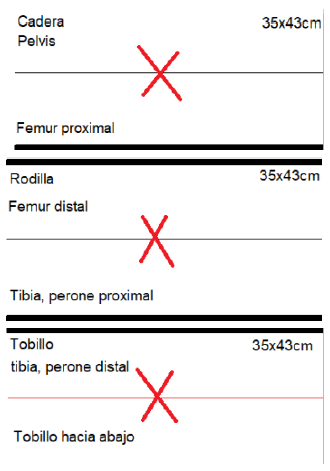
\includegraphics[width=0.7\linewidth]{imagenes/medi7}
		\caption{División del chasis}
		\label{fig:medi7}
	\end{figure}
	
	\onecolumn
	\clearpage
	
	\begin{figure}
		\centering
		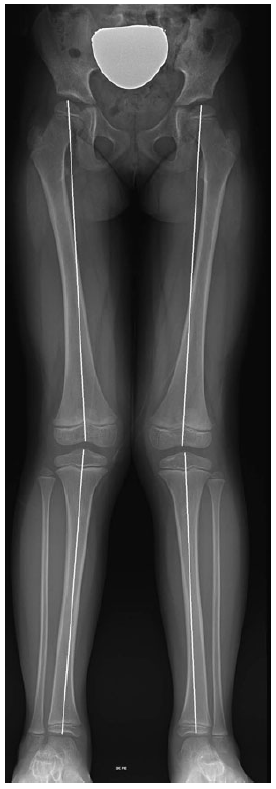
\includegraphics[width=0.5
		\linewidth]{imagenes/medi8}
		\caption{}
		\label{fig:medi8}
	\end{figure}
	
	
	\twocolumn
	\clearpage
	%----------------------------------------------------------
	%  Para agregar otro enfoque duplicá el bloque
	%  desde \subsection hasta \textbf{Trucos}
	%----------------------------------------------------------
	
	

	\clearpage
\onecolumn
\thispagestyle{empty}
\vspace*{\fill}
\begin{center}
	{\color{radblue}\rule{\linewidth}{2pt}}\par
	\vspace{6mm}
	{\Huge\bfseries\color{radblue}Columna}\par
	\vspace{6mm}
	{\color{radblue}\rule{\linewidth}{2pt}}
\end{center}
\vspace*{\fill}
\clearpage
\twocolumn
\pagestyle{contenido}



%%%%%%%%%%%%%%%%%%%%%%%%%%%%%%%%%%%%%%%%%%%%%%%%%%%%%%%%%%%
%  SECCIÓN: Columna Cervical — Articulación Atlanto-Axoidea
%  Archivo: secciones/columna_cervical.tex
%  Sin preámbulo ni \begin{document} — lo maneja main.tex
	%%%%%%%%%%%%%%%%%%%%%%%%%%%%%%%%%%%%%%%%%%%%%%%%%%%%%%%%%%%
	
	\section{Columna Cervical}
	
	\subsection{Articulación Atlanto-Axoidea - Enfoque Transbucal (Boca Abierta)}
	
	\subsubsection*{1. Identificación}
	
	\textbf{Tipo:} Proyección complementaria.
	
	\textbf{Indicaciones clínicas principales:}
	\begin{itemize}
		\item Traumatismo cervical alto: fractura de Jefferson (C1) y fractura de apófisis odontoides (C2)
		\item Fracturas de masas laterales de C1
		\item Cervicalgia, artritis reumatoidea con sospecha de subluxación del ligamento transverso
		\item Pacientes politraumatizados por accidentes de tránsito
		\item Luxaciones atlanto-axoideas e inestabilidad C1-C2
	\end{itemize}
	
	\subsubsection*{2. Técnica Base}
	
	\textbf{Receptor de imagen:} 18$\times$24 cm o 24$\times$30 cm. Orientación \textbf{longitudinal}, centrado a la altura del axis.
	
	\textbf{DFRI:} 70 cm (preferencial). Se aprovecha la divergencia del rayo: con el tubo más cerca, el haz permite proyectar la base del cráneo hacia arriba y los dientes fuera del campo, despejando la odontoides en el centro del receptor. Puede utilizarse hasta 1 metro, pero siempre menos de ese valor.
	
	\textbf{Técnica:} Intermedia (homogeneizada). La boca actúa como ventana natural, lo que resulta suficiente para obtener detalle de la odontoides, valorar el trabeculado óseo y detectar líneas de fractura cuando existieran.
	
	\textbf{Bucky:} Bucky de mesa con grilla.
	
	\subsubsection*{3. Posicionamiento}
	
	\paragraph{Paciente}
	Decúbito supino. Brazos a los lados del cuerpo; puede colocarse un apoyo bajo las rodillas para mayor comodidad. El plano medio sagital debe estar perpendicular y centrado en línea media respecto al receptor.
	
	\begin{figure}[h]
		\centering
		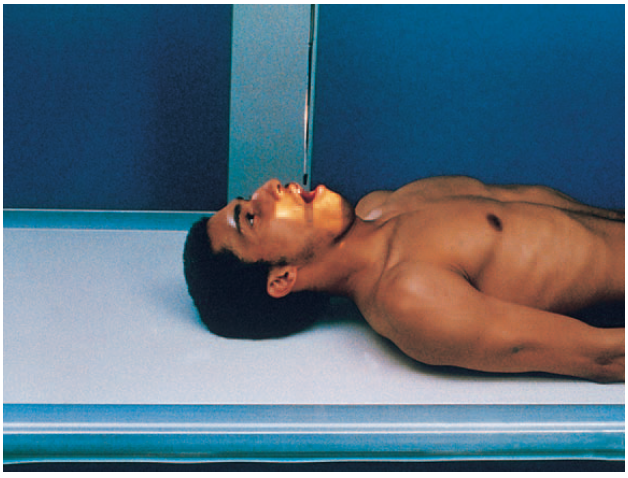
\includegraphics[width=0.7\linewidth]{imagenes/col1}
		\caption{}
		\label{fig:col1}
	\end{figure}
	
	
	\paragraph{Región de interés}
	Se ajusta la cabeza de manera que el \textbf{plano de oclusión} —línea trazada entre el borde inferior de los incisivos superiores y el vértice de la apófisis mastoides— quede \textbf{perpendicular al receptor de imagen}. Los hombros deben permanecer en el mismo plano horizontal. Se le pide al paciente que abra la boca al máximo.
	
	\paragraph{Rayo Central}
	Perpendicular al plano del receptor. Punto de entrada: \textbf{punto medio de la boca abierta}.
	
	\paragraph{Receptor de imagen}
	Centrado a la altura del axis (C2). La región a incluir abarca desde el borde inferior de los incisivos superiores hasta el borde superior del mentón (para asegurar el cuerpo de C2), y lateralmente las ramas mandibulares. Colimación ajustada a los cuatro lados del área de interés, aproximadamente 10$\times$10 cm.
	
	\paragraph{Respiración}
	Durante la exposición, indicar al paciente que mantenga la boca abierta y diga suavemente \textit{``ah''} de forma sostenida. La fonación hace que la lengua descienda y quede quieta, evitando su superposición sobre C1-C2 y previniendo la generación de imágenes falsas (pseudofracturas). Se le indica además que no respire ni trague durante la exposición.
	
	\subsubsection*{4. Anatomía Visible}
	
	Se visualizan la apófisis odontoides (C2), el atlas (C1) con sus masas laterales, el cuerpo del axis y las articulaciones atlanto-axoideas (C1-C2) a través de la cavidad bucal. Deben verse todas las superficies articulares del atlas y el axis para permitir la comprobación de desplazamiento lateral. Las ramas mandibulares deben proyectarse equidistantes respecto a la odontoides. La sombra de la lengua no debe superponerse sobre el atlas ni el axis.
	
	\subsubsection*{5. Criterios de Evaluación}
	
	\textbf{Posicionamiento correcto:} Odontoides visible sin superposición en el centro de la imagen. Borde inferior de los incisivos superiores y la base del cráneo alineados y ubicados por encima de la punta de la odontoides. Ramas mandibulares equidistantes. Boca bien abierta. Sombra de la lengua no proyectada sobre C1-C2. La posición es óptima cuando las sombras de la superficie de oclusión de los incisivos centrales superiores, la base del cráneo y los vértices de las apófisis mastoides se encuentran en línea.
	
	\textbf{Ausencia de rotación:} El espacio entre la odontoides y las masas laterales de C1 debe ser igual de ambos lados. Si un lado se observa más ancho que el otro, el paciente está rotado. El plano medio sagital (línea que pasa por nariz y mentón) debe quedar perpendicular al receptor sin desviación lateral.
	
	\textbf{Penetración y contraste:} Técnica intermedia que permite valorar el trabeculado óseo de la odontoides y detectar líneas de fractura finas. La imagen debe mostrar contraste suficiente para diferenciar las corticales de C1 y C2 del espacio articular y los tejidos blandos circundantes.
	
	\subsubsection*{6. Puntos Críticos}
	
	\textbf{Incisivos superiores superpuestos a la odontoides (mentón muy bajo):} Los dientes tapan la odontoides y pueden simular una línea de fractura (pseudofractura). Corrección: subir levemente el mentón aumentando la extensión de la cabeza.
	
	\textbf{Base del cráneo (occipital) superpuesta a la odontoides (mentón muy elevado):} La nuca cubre la odontoides impidiendo su valoración. Corrección: bajar levemente el mentón reduciendo la extensión.
	
	\textbf{Adaptaciones:} En pacientes con traumatismo cervical no debe intentarse ningún movimiento sin autorización médica previa. Antes de realizar este estudio debe haberse obtenido una radiografía lateral con rayo central horizontal para descartar inestabilidad. Si no se logra un enfoque adecuado luego de dos intentos, se debe recurrir a métodos alternativos como el enfoque de Fuchs o de Judd.
	
	\textbf{Trucos:} La fonación sostenida con \textit{``ah''} es el recurso más efectivo para inmovilizar la lengua y evitar pseudofracturas. La DFRI de 70 cm (menor de 1 metro) es clave: aprovecha la divergencia del haz para despejar la base del cráneo y los dientes del campo de la odontoides. Recordar siempre que este es un \textbf{enfoque complementario} que requiere correlación con la proyección lateral cervical.
	
	\onecolumn
	\clearpage
	
	\begin{figure}
		\centering
		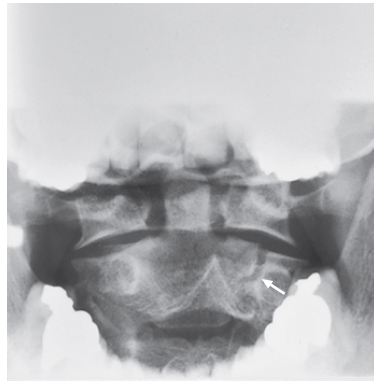
\includegraphics[width=0.7\linewidth]{imagenes/col2}
		\caption{Fractura en masa lateral}
		\label{fig:col2}
	\end{figure}
	
	\twocolumn
	\clearpage
	
	%----------------------------------------------------------
	%  Para agregar otro enfoque duplicá el bloque
	%  desde \subsection hasta \textbf{Trucos}
	%----------------------------------------------------------
	
	
	%%%%%%%%%%%%%%%%%%%%%%%%%%%%%%%%%%%%%%%%%%%%%%%%%%%%%%%%%%%
	%  SECCIÓN: Columna Cervical
	%  Archivo: secciones/columna_cervical.tex
	%  Sin preámbulo ni \begin{document} — lo maneja main.tex
		%%%%%%%%%%%%%%%%%%%%%%%%%%%%%%%%%%%%%%%%%%%%%%%%%%%%%%%%%%%
		
	\section{Columna Cervical}
		
		\subsection{Odontoides AP - Método de Fuchs}
		
		\subsubsection*{1. Identificación}
		
		\textbf{Tipo:} Proyección complementaria.
		
		\textbf{Indicaciones clínicas principales:}
		\begin{itemize}
			\item Artrosis severa que impida la apertura bucal para la proyección transoral.
			\item Trismo (limitación de la apertura bucal).
			\item Paciente con collarín cervical que no puede abrir la boca.
			\item Demostración de la odontoides cuando la mitad superior no se visualiza con claridad en boca abierta.
			\item Inestabilidad atlanto-axoidea.
		\end{itemize}
		
		\textbf{Contraindicación absoluta:} No intentar esta posición ante sospecha de trauma agudo. La extensión forzada del cuello puede desplazar una fractura inestable y causar daño neurológico permanente. Las fracturas de odontoides (Jefferson) están contraindicadas.
		
		\subsubsection*{2. Técnica Base}
		
		\textbf{Receptor de imagen:} 18$\times$24 cm (o 24$\times$30 cm). Orientación \textbf{transversal} centrado a la altura de los vértices de las apófisis mastoides.
		
		\textbf{DFRI:} 100 cm. Distancia estándar para proyecciones de columna cervical.
		
		\textbf{Técnica:} Homogeneizada. El rayo central debe atravesar la base del cráneo, estructura de alta densidad; se requiere un kVp elevado para penetrar y homogeneizar las densidades y visualizar la odontoides por transparencia con nitidez.
		
		\textbf{Bucky:} Bucky de mesa con grilla.
		
		\subsubsection*{3. Posicionamiento}
		
		\paragraph{Paciente}
		Decúbito supino sobre la mesa. Brazos extendidos a los lados del cuerpo. Hombros ajustados para que queden en el mismo plano horizontal. Se puede colocar un apoyo bajo las rodillas para mayor comodidad del paciente.
		
		\begin{figure}[h]
			\centering
			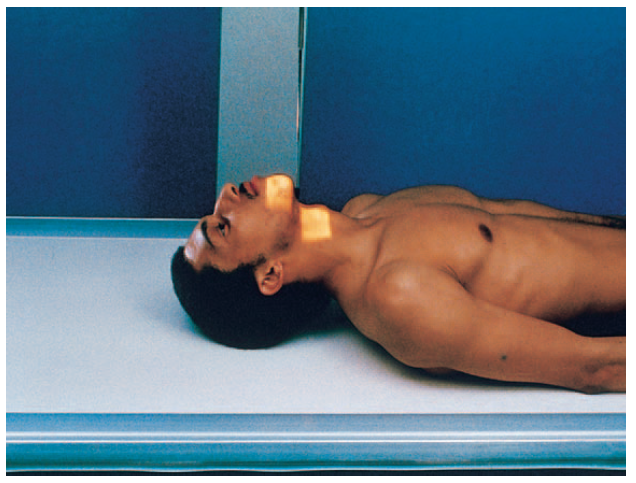
\includegraphics[width=0.7\linewidth]{imagenes/col3}
			\caption{}
			\label{fig:col3}
		\end{figure}
				
		\paragraph{Región de interés}
		El paciente eleva el mentón hasta que la línea mento-meatal (trazada desde el conducto auditivo externo hasta el mentón) quede perpendicular al receptor de imagen. El plano medio sagital debe quedar perpendicular y centrado respecto al RI.
		
		\paragraph{Rayo Central}
		Perpendicular al plano del receptor. Punto de entrada: \textbf{plano medio sagital, inmediatamente distal (inferior) al vértice del mentón}. Si el paciente no puede lograr que la línea mento-meatal quede perpendicular al RI, se angula el RC en dirección craneal de modo que siga incidiendo por debajo del vértice del mentón, compensando la falta de extensión.
		
		\paragraph{Receptor de imagen}
		Centrado a la altura de los vértices de las apófisis mastoides. La colimación se ajusta por los cuatro lados a la región C1--C2. La región a incluir comprende: borde superior del agujero occipital, cuerpo completo de C2 y ángulos mandibulares (para verificar el centrado).
		
		\paragraph{Respiración}
		Suspendida en espiración, sin deglutir. Se instruye al paciente a no respirar ni tragar durante la exposición para evitar cualquier movimiento que genere borrosidad en la imagen.
		
		\subsubsection*{4. Anatomía Visible}
		
		La estructura principal a demostrar es la \textbf{apófisis odontoides de C2 completa}, enmarcada dentro del agujero occipital (agujero magno), que actúa como \textbf{ventana radiológica}: espacio delimitado que forma una cavidad a través de la cual se valora la odontoides por transparencia. Se visualizan también la relación espacial entre la odontoides y el agujero magno, y los ángulos mandibulares como referencias de simetría y centrado.
		
		\subsubsection*{5. Criterios de Evaluación}
		
		\textbf{Posicionamiento correcto:} Toda la apófisis odontoides debe estar enmarcada dentro del agujero magno circular. El RC ha incidido inmediatamente distal al vértice del mentón en el PMS.
		
		\textbf{Ausencia de rotación:} Los ángulos mandibulares deben aparecer equidistantes respecto a la apófisis odontoides y respecto a la línea media del RI. El lado que se vea más ancho corresponde al lado menos apoyado. La nariz y el mentón deben estar alineados con la línea media del chasis.
		
		\textbf{Penetración y contraste:} Técnica homogeneizada que permita ver la odontoides con nitidez por detrás de la base del cráneo; densidades equilibradas entre las estructuras óseas superpuestas.
		
		\subsubsection*{6. Puntos Críticos}
		
		\textbf{Falta de extensión (mentón cubre la odontoides):} El mentón superpone la odontoides impidiendo su visualización. Corrección: indicar al paciente que eleve más el mentón, o angular el RC en dirección craneal para que incida igualmente distal al vértice del mentón.
		
		\textbf{Exceso de extensión (base del cráneo cubre la odontoides):} La base del cráneo se superpone sobre la odontoides. Corrección: indicar al paciente que baje el mentón hasta recuperar la posición correcta de la línea mento-meatal.
		
		\textbf{Adaptaciones:} En pacientes con limitación para extender el cuello (collarín, rigidez, posquirúrgico), compensar angulando el RC cranealmente en lugar de forzar la extensión cervical. No intentar la proyección en trauma agudo con sospecha de fractura inestable.
		
		\textbf{Trucos:} La ventana radiológica del agujero magno es el concepto clave de esta proyección: no se visualiza la odontoides directamente, sino \textit{por transparencia} a través del agujero occipital. Recordar que la línea mento-meatal (CAE--mentón) perpendicular al RI es el eje de posicionamiento central, y que la angulación del RC es el recurso corrector cuando el paciente no puede lograrlo anatómicamente.
		
		
		\onecolumn
		\clearpage
		
		\begin{figure}
			\centering
			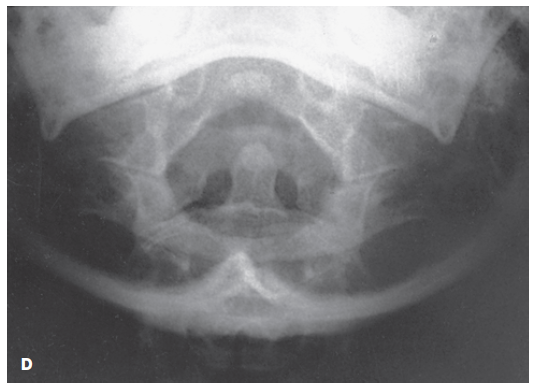
\includegraphics[width=0.7\linewidth]{imagenes/col4}
			\caption{}
			\label{fig:col4}
		\end{figure}
		
		
		\twocolumn
		\clearpage
		%----------------------------------------------------------
		%  Para agregar otro enfoque duplicá el bloque
		%  desde \subsection hasta \textbf{Trucos}
		%----------------------------------------------------------
	
	%%%%%%%%%%%%%%%%%%%%%%%%%%%%%%%%%%%%%%%%%%%%%%%%%%%%%%%%%%%
	%  SECCIÓN: Columna Cervical
	%  Archivo: secciones/columna_cervical.tex
	%  Sin preámbulo ni \begin{document} — lo maneja main.tex
		%%%%%%%%%%%%%%%%%%%%%%%%%%%%%%%%%%%%%%%%%%%%%%%%%%%%%%%%%%%
		
	\section{Columna Cervical}
		
		\subsection{Odontoides PA - Método de Judd}
		
		\subsubsection*{1. Identificación}
		
		\textbf{Tipo:} Proyección complementaria. Posición inversa al Método de Fuchs; ambos métodos son alternativas cuando el paciente no puede realizar la proyección transoral.
		
		\textbf{Indicaciones clínicas principales:}
		\begin{itemize}
			\item Demostración y evaluación de la apófisis odontoides
			\item Fracturas de odontoides y estructuras óseas circundantes de C1
			\item Alternativa al Método de Fuchs en pacientes con limitaciones (ej.\ trauma, collarín cervical)
			\item Alternativa a la proyección transoral cuando el paciente no puede abrir la boca
		\end{itemize}
		
		\subsubsection*{2. Técnica Base}
		
		\textbf{Receptor de imagen:} 18$\times$24 cm (o 24$\times$30 cm). Orientación \textbf{transversal} para incluir la región C1--C2 en su totalidad.
		
		\textbf{DFRI:} 100 cm. Distancia estándar para proyecciones de columna cervical.
		
		\textbf{Bucky:} Bucky de mesa. Técnica homogeneizada.
		
		\subsubsection*{3. Posicionamiento}
		
		\paragraph{Paciente}
		Decúbito prono sobre la mesa. Manos apoyadas sobre la mesa a los lados de la cabeza. El plano medio sagital debe quedar perpendicular al receptor para evitar rotación.
		
		\begin{figure}[h]
			\centering
			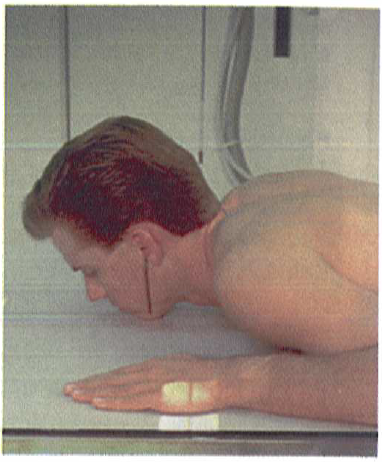
\includegraphics[width=0.7\linewidth]{imagenes/col5}
			\caption{}
			\label{fig:col5}
		\end{figure}
		
		
		\paragraph{Región de interés}
		El mentón descansa directamente sobre la superficie de la mesa. Se extiende la cabeza hasta que la línea mento-meatal (LMM) quede casi perpendicular a la mesa. La LMM une el mentón con el meato auditivo externo. El rayo central puede ajustarse según las necesidades del paciente para mantenerse paralelo a la LMM. Verificar ausencia de rotación de cabeza y cuello.
		
		\paragraph{Rayo Central}
		Paralelo a la línea mento-meatal (LMM). Punto de entrada: \textbf{a través del hueso occipital medio, aproximadamente 2,5 cm inferoposterior a las puntas de las apófisis mastoides y ángulos mandibulares}. Angulación referencial de 20° en vista lateral según necesidad del paciente.
		
		\paragraph{Receptor de imagen}
		Centrado en la región C1--C2. Colimación ajustada por los cuatro lados para incluir toda la odontoides enmarcada en el agujero magno.
		
		\paragraph{Respiración}
		Suspendida. Instruir al paciente que no respire ni trague durante la exposición, para evitar artefactos de movimiento en la región cervical superior.
		
		\subsubsection*{4. Anatomía Visible}
		
		Apófisis odontoides (proceso odontoideo), atlas (C1) y axis (C2). Relación atlanto-axoidea. La odontoides debe aparecer enmarcada dentro del agujero magno. Estructuras de referencia visibles: mandíbula con sus ángulos (gonios) y la V mandibular, cráneo y vértebras cervicales superiores.
		
		\subsubsection*{5. Criterios de Evaluación}
		
		\textbf{Posicionamiento correcto:} La apófisis odontoides queda completamente enmarcada dentro del agujero magno, visible en su totalidad sin superposiciones óseas que la oculten.
		
		\textbf{Ausencia de rotación:} Simetría bilateral de la mandíbula, del cráneo y de las vértebras cervicales; los ángulos mandibulares (gonios) deben verse equidistantes respecto al plano medio. La asimetría indica rotación de cabeza o cuello.
		
		\textbf{Penetración y contraste:} Técnica homogeneizada adecuada para visualizar la odontoides diferenciada del occipucio y las estructuras circundantes.
		
		\subsubsection*{6. Puntos Críticos}
		
		\textbf{Rotación de la cabeza o el cuello:} Genera asimetría mandibular y vertebral; la odontoides se desplaza del centro del agujero magno. Corregir reposicionando al paciente con el plano medio sagital estrictamente perpendicular al RI.
		
		\textbf{LMM no perpendicular a la mesa:} Si la extensión es insuficiente, la mandíbula se superpone sobre la odontoides. Ajustar el rayo central para que quede paralelo a la LMM o aumentar la extensión cervical dentro de las posibilidades del paciente.
		
		\textbf{Adaptaciones:} En pacientes con trauma o collarín cervical que no pueden abrir la boca (proyección transoral contraindicada), el Método de Judd en decúbito prono y el Método de Fuchs en decúbito supino son las alternativas de elección. Puede realizarse también en bipedestación.
		
		\textbf{Trucos:} La diferencia fundamental con el Método de Fuchs es la posición del paciente: Judd en decúbito prono (PA) y Fuchs en decúbito supino (AP). En el Judd el mentón contacta directamente la mesa. El método transoral sigue siendo el ideal, ya que permite ver además las masas laterales del atlas; Judd y Fuchs se usan cuando la boca cerrada es la única opción disponible.
		
		
			\onecolumn
		\clearpage
		
		\begin{figure}
			\centering
			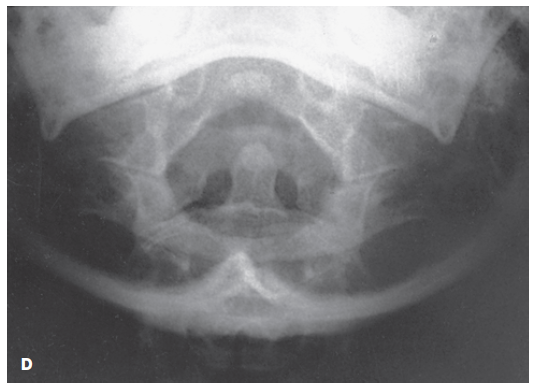
\includegraphics[width=0.7\linewidth]{imagenes/col4}
			\caption{}
			\label{fig:col4}
		\end{figure}
		
		
		\twocolumn
		\clearpage
		
		%----------------------------------------------------------
		%  Para agregar otro enfoque duplicá el bloque
		%  desde \subsection hasta \textbf{Trucos}
		%----------------------------------------------------------
		
		
	%%%%%%%%%%%%%%%%%%%%%%%%%%%%%%%%%%%%%%%%%%%%%%%%%%%%%%%%%%%
	%  SECCIÓN: Columna Cervical
	%  Archivo: secciones/columna_cervical.tex
	%  Sin preámbulo ni \begin{document} — lo maneja main.tex
		%%%%%%%%%%%%%%%%%%%%%%%%%%%%%%%%%%%%%%%%%%%%%%%%%%%%%%%%%%%
		
	\section{Columna Cervical}
		
		\subsection{Frente de Columna Cervical (AP)}
		
		\subsubsection*{1. Identificación}
		
		\textbf{Tipo:} Proyección básica. Forma par con el perfil de columna cervical (RC horizontal).
		
		\textbf{Indicaciones clínicas principales:}
		\begin{itemize}
			\item Cervicalgia y rectificación cervical
			\item Hernia del núcleo pulposo (HNP) con radiculopatía cervical
			\item Traumatismo de tránsito (latigazo cervical, fractura de apófisis espinosa — ``cavador de arcilla'')
			\item Fracturas por compresión vertebral
		\end{itemize}
		
		\subsubsection*{2. Técnica Base}
		
		\textbf{Receptor de imagen:} 18$\times$24 cm (o 24$\times$30 cm). Orientación \textbf{longitudinal} adaptada según biotipo del paciente.
		
		\textbf{DFRI:} 100 cm. Distancia estándar para proyecciones axiales de columna, reduce distorsión geométrica y mantiene definición.
		
		\textbf{Técnica:} Homogeneizada (escala larga). Se emplea suficiente kVp para visualizar simultáneamente tejidos blandos (vía aérea, laringe), detalle óseo (trabeculado y cortical) y espacios intervertebrales en una sola imagen.
		
		\textbf{Bucky:} Sí. Se utiliza Bucky mural (bipedestación) o Bucky de mesa (decúbito supino).
		
		\subsubsection*{3. Posicionamiento}
		
		\paragraph{Paciente}
		Decúbito supino o bipedestación (descalzo). Espalda apoyada contra el receptor. Hombros ubicados en el mismo plano horizontal y paralelos al RI para evitar curvatura lateral aparente de la columna. El plano medio sagital debe ser perpendicular al receptor.
		
		\begin{figure}[h]
			\centering
			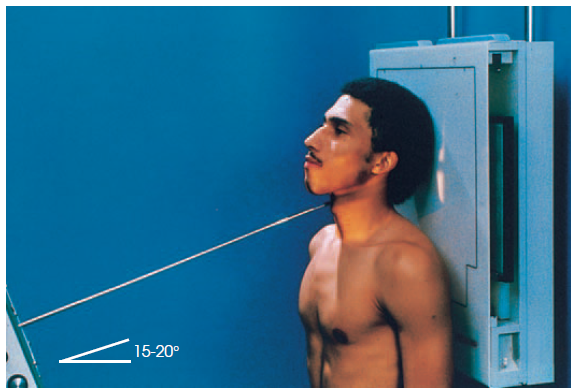
\includegraphics[width=0.7\linewidth]{imagenes/col7}
			\caption{}
			\label{fig:col7}
		\end{figure}
				
		\paragraph{Región de interés}
		Se eleva ligeramente el mentón para superponer el occipital con el mentón y evitar que la mandíbula se proyecte sobre las vértebras cervicales. Diferencia de posición occipital-mentón: aproximadamente 0,5 cm. En pacientes con lordosis pronunciada se provee apoyo bajo la cabeza. Referencia práctica: 2 dedos sobre el occipital y 1 dedo por delante del mentón.
		
		\paragraph{Rayo Central}
		Angulado \textbf{15--20° craneal} al plano del receptor. La angulación permite que el haz pase tangencial a los espacios intervertebrales, compensando la lordosis cervical. Punto de entrada: \textbf{C4 (por encima de la nuez de Adán)}. Si se logra correcta superposición anatómica occipital-mentón se angula 15°; si no se logra, se angula 20° (mayor angulación desplaza estructuras y puede comprometer la superposición ya lograda).
		
		\paragraph{Receptor de imagen}
		Centrado en C4. El borde superior se ubica a nivel del conducto auditivo externo (CAE) y el borde inferior debe incluir hasta T2--T3 (pasaje torácico). La región abarca de C3 a T2--T3.
		
		\paragraph{Respiración}
		Suspendida. Se indica al paciente que no respire y no degluta durante la exposición, para evitar movimiento a nivel de la vía aérea (laringe, tráquea) que genere borrosidad en las estructuras blandas del cuello.
		
		\subsubsection*{4. Anatomía Visible}
		
		Se visualizan los cuerpos vertebrales de C3 a C7 y T1--T3 con sus espacios discales intervertebrales abiertos. El Atlas (C1) y la mayor parte del Axis (C2) quedan superpuestos por el occipital y la mandíbula. Las apófisis transversas y articulares aparecen superpuestas entre sí. Son visibles la laringe, la tráquea y tejidos blandos prelaríngeos gracias a la técnica homogeneizada. Las clavículas deben verse paralelas entre sí y simétricas respecto a la columna.
		
		\subsubsection*{5. Criterios de Evaluación}
		
		\textbf{Posicionamiento correcto:} Espacios intervertebrales abiertos y nítidos gracias a la angulación craneal. Mandíbula y base del cráneo superpuestos a C1--C2. Cuerpos vertebrales de C3 hacia abajo claramente individualizados. Clavículas paralelas y simétricas respecto a la columna.
		
		\textbf{Ausencia de rotación:} Apófisis espinosas equidistantes y alineadas con la línea media de los cuerpos vertebrales. Ángulos mandibulares y apófisis mastoides equidistantes entre sí. Cualquier desviación de las apófisis espinosas indica rotación de cabeza o tronco; corregir con el PMS.
		
		\textbf{Penetración y contraste:} Técnica homogeneizada: escala larga con kVp suficiente para demostrar simultáneamente tejido blando (vía aérea, laringe) y detalle óseo (trabeculado, cortical, espacios intervertebrales) en una sola imagen.
		
		\subsubsection*{6. Puntos Críticos}
		
		\textbf{Superposición mandibular excesiva:} El mentón muy bajo proyecta los gonios mandibulares sobre las vértebras superiores, ocultando C3. Se identifica porque la mandíbula aparece cuadrada con gonios visibles. Corrección: elevar el mentón hasta lograr superposición occipital-mentón adecuada.
		
		\textbf{Occipital demasiado posterior:} El hueso occipital se proyecta redondeado sobre la columna (imagen en V), tapando C3. Corrección: ajustar posición del occipital y mentón en diferencia de 0,5 cm.
		
		\textbf{Adaptaciones:} En trauma de tránsito el estudio se realiza en decúbito supino sin movilizar al paciente. El complementario transoral es prioritario cuando el paciente porta collarín cervical. No se realizan estudios funcionales en contexto de traumatismo agudo.
		
		\textbf{Trucos:} La angulación cefálica dirige el haz entre cuerpos vertebrales superpuestos por la lordosis. Contar vértebras desde C7 hacia arriba (la prominente es el punto de referencia), ya que C1--C2 quedan bajo el cráneo. Si la colimación llega a T3--T4 puede reducirse. Para rectificación cervical o cervicalgia el estudio se complementa con funcionales (hiperextensión e hiperflexión) como proyecciones complementarias.
		
		\onecolumn
		\clearpage
		
		\begin{figure}
			\centering
			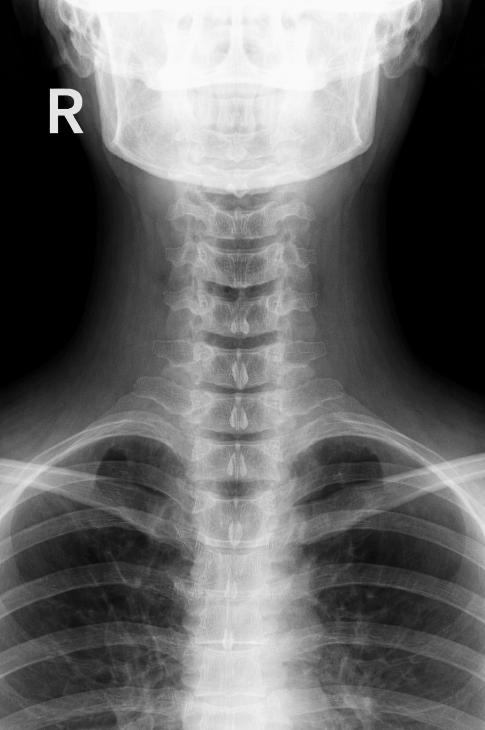
\includegraphics[width=0.7\linewidth]{imagenes/col6}
			\caption{}
			\label{fig:col6}
		\end{figure}
		
		
		\twocolumn
		\clearpage
		
		
		
		%----------------------------------------------------------
		%  Para agregar otro enfoque duplicá el bloque
		%  desde \subsection hasta \textbf{Trucos}
		%----------------------------------------------------------
		
		
	%%%%%%%%%%%%%%%%%%%%%%%%%%%%%%%%%%%%%%%%%%%%%%%%%%%%%%%%%%%
	%  SECCIÓN: Columna Cervical
	%  Archivo: secciones/columna_cervical.tex
	%  Sin preámbulo ni \begin{document} — lo maneja main.tex
		%%%%%%%%%%%%%%%%%%%%%%%%%%%%%%%%%%%%%%%%%%%%%%%%%%%%%%%%%%%
		
	\section{Columna Cervical}
		
		\subsection{Proyección Lateral de Columna Cervical (Método de Grandy)}
		
		\subsubsection*{1. Identificación}
		
		\textbf{Tipo:} Proyección básica. Forma par con la proyección anteroposterior de columna cervical.
		
		\textbf{Indicaciones clínicas principales:}
		\begin{itemize}
			\item Cervicalgia y discopatías (sospecha de hernia de disco / hernias del núcleo pulposo con pinzamiento radicular)
			\item Rectificación cervical y espondiloartrosis (visualización de osteofitos y desgaste articular)
			\item Traumatismo de tránsito: latigazo, fractura de apófisis espinosa (fractura del cavador de arcilla)
			\item Parestesias (hormigueos) de origen cervical
		\end{itemize}
		
		\subsubsection*{2. Técnica Base}
		
		\textbf{Receptor de imagen:} 18$\times$24 cm (puede utilizarse 24$\times$30 cm). Orientación \textbf{longitudinal} (vertical). El borde superior del receptor se ubica 2,5 cm por encima del conducto auditivo externo (C.A.E.).
		
		\textbf{DFRI:} 140 cm (1,52--1,83 m). La distancia aumentada compensa la separación entre la columna cervical y el receptor impuesta por la presencia de los hombros: los rayos llegan más paralelos y menos divergentes, se reduce la magnificación y se minimiza la distorsión geométrica. El incremento de distancia requiere multiplicar los mAs por 2 respecto a la técnica estándar.
		
		\textbf{Técnica:} Homogeneizada (escala larga). Suficiente kVp para demostrar simultáneamente el tejido blando (vías aéreas, laringe) y el detalle óseo (trabeculado, cortical) junto con los espacios intervertebrales en una sola imagen.
		
		\textbf{Bucky:} Bucky con grilla.
		
		\subsubsection*{3. Posicionamiento}
		
		\paragraph{Paciente}
		Bipedestación o sentado en posición lateral estricta. El plano medio sagital queda paralelo al receptor. Los hombros se desplazan hacia abajo tanto como sea posible (en la práctica: pedir al paciente que tome sus propias manos por detrás de la espalda y baje los hombros, o utilizar pesos en las muñecas). Ambos hombros deben quedar en el mismo plano horizontal para evitar rotación del tronco.
		
		\begin{figure}[h]
			\centering
			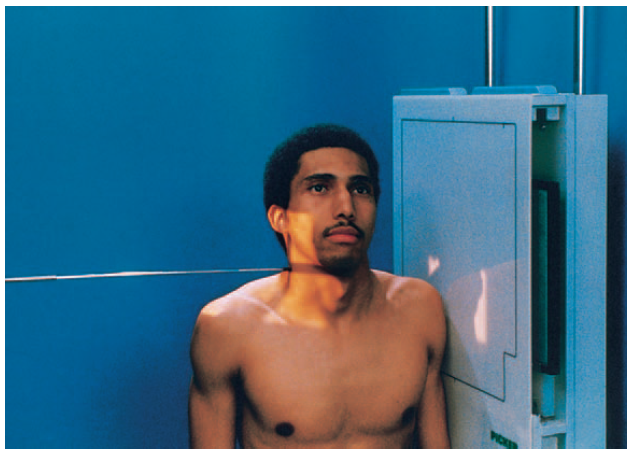
\includegraphics[width=0.7\linewidth]{imagenes/col8}
			\caption{}
			\label{fig:col8}
		\end{figure}
		
		
		\paragraph{Región de interés}
		La barbilla se eleva para que las ramas y los ángulos de la mandíbula no se superpongan a C1--C2. El paciente fija la mirada en un punto de la pared para mantener la posición y evitar rotación cervical. El plano medio sagital permanece paralelo al receptor durante toda la exposición.
		
		\paragraph{Rayo Central}
		Horizontal y perpendicular al plano del receptor. Punto de entrada: \textbf{C4, a nivel de la parte superior del cartílago tiroides}.
		
		\paragraph{Receptor de imagen}
		Centrado en C4. El borde superior queda 2,5 cm por encima del C.A.E. La colimación abarca 4 cm a cada lado del cuello. La región incluida comprende los cuerpos vertebrales desde C1 hasta C7, con al menos un tercio de T1 visible.
		
		\paragraph{Respiración}
		Suspendida al final de una espiración máxima. Este momento logra el máximo descenso de los hombros, favoreciendo la visualización de C7 y T1 sin superposición.
		
		\subsubsection*{4. Anatomía Visible}
		
		Las siete vértebras cervicales en perfil estricto y al menos un tercio de T1. Cuerpos vertebrales con morfología lateral sin doble contorno. Apófisis espinosas de perfil. Pilares articulares. Espacios discales intervertebrales abiertos y radiolúcidos. Cinco articulaciones interapofisarias inferiores abiertas y superpuestas entre sí (indicativo de ausencia de rotación). Tejidos blandos adyacentes: vías aéreas, laringe.
		
		\subsubsection*{5. Criterios de Evaluación}
		
		\textbf{Posicionamiento correcto:} Barbilla elevada de modo que las ramas y los ángulos mandibulares no se superpongan a C1--C2. C4 en el centro de la imagen. Las ramas mandibulares se proyectan superpuestas o casi superpuestas entre sí (un leve desfase es normal por diferencia de magnificación entre la rama más cercana y la más lejana al receptor). Apófisis espinosas de perfil.
		
		\textbf{Ausencia de rotación:} Articulaciones interapofisarias superpuestas y abiertas. Cuerpos vertebrales de perfil sin doble contorno. Si existe rotación, las ramas mandibulares aparecen desplazadas: una posterior y otra anterior. Si existe inclinación lateral, una rama queda superior y la otra inferior.
		
		\textbf{Penetración y contraste:} Escala larga (alto kVp) que permite visualizar simultáneamente el detalle óseo (trabeculado y cortical) y los tejidos blandos cervicales (vías aéreas, laringe) en una sola imagen. Espacios discales intervertebrales perceptibles y radiolúcidos.
		
		\subsubsection*{6. Puntos Críticos}
		
		\textbf{Elevación de hombros:} Impide la visualización de C7 y T1 por superposición. Corrección: pedir al paciente que baje los hombros activamente, utilizar pesos en las muñecas o indicar que tome sus manos por detrás; si C7 no es visible, obtener una proyección cervicotorácica separada.
		
		\textbf{Rotación cervical:} Las ramas mandibulares se proyectan desfasadas (una anterior y otra posterior) y los cuerpos vertebrales muestran doble contorno. Corrección: verificar que el plano medio sagital sea estrictamente paralelo al receptor y pedir al paciente que mire un punto fijo en la pared.
		
		\textbf{Adaptaciones:} Si el paciente no puede bajar los hombros voluntariamente, se utilizan pesos sujetos a las muñecas. En pacientes con inclinación lateral que cierra los espacios articulares, corregir dejando el plano medio sagital paralelo al receptor (ajustar el PMS).
		
		\textbf{Trucos:} Las ramas mandibulares siempre quedan levemente desfasadas entre sí por diferencia de magnificación (distinta distancia al receptor); este desfase leve es normal y no debe confundirse con rotación. Para contar las vértebras se procede de arriba hacia abajo. El paciente que fija la mirada en un punto fijo de la pared mantiene mejor la posición y reduce la necesidad de repetir la exposición.
		
		\onecolumn
		\clearpage
		
		\begin{figure}
			\centering
			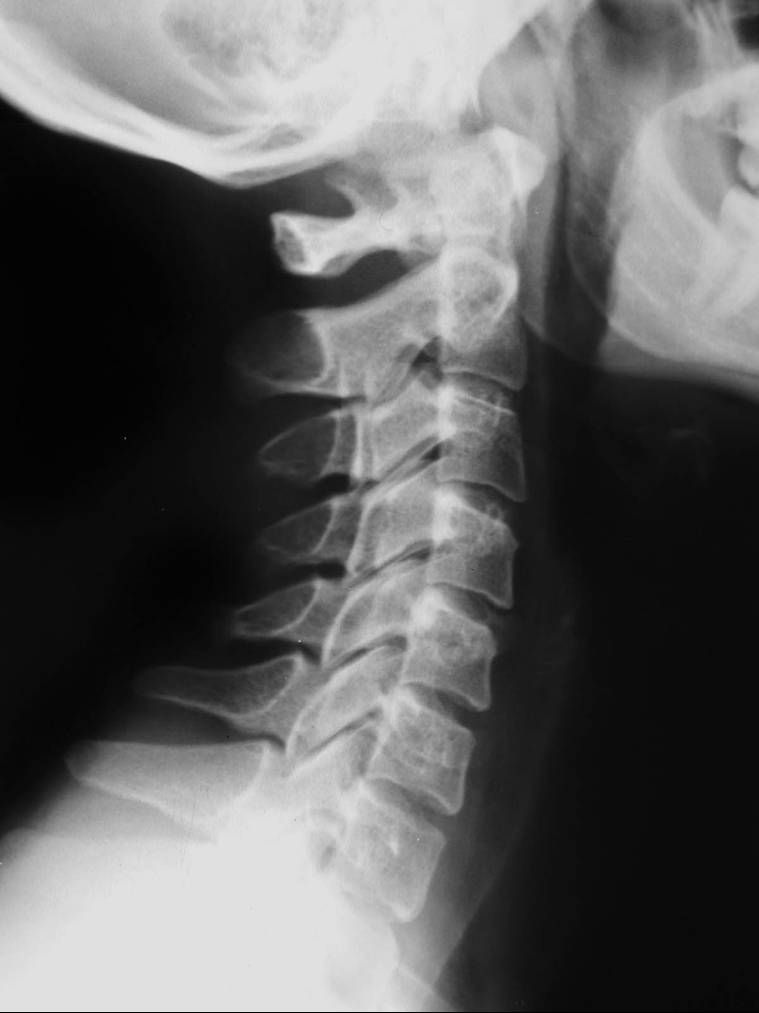
\includegraphics[width=0.7\linewidth]{imagenes/col9}
			\caption{}
			\label{fig:col9}
		\end{figure}
		
		
		\twocolumn
		\clearpage
		
		
		%----------------------------------------------------------
		%  Para agregar otro enfoque duplicá el bloque
		%  desde \subsection hasta \textbf{Trucos}
		%----------------------------------------------------------
		
		
		
%%%%%%%%%%%%%%%%%%%%%%%%%%%%%%%%%%%%%%%%%%%%%%%%%%%%%%%%%%%
%  SECCIÓN: Columna Cervical
%  Archivo: secciones/funcionales_cervical.tex
%  Sin preámbulo ni \begin{document} — lo maneja main.tex
	%%%%%%%%%%%%%%%%%%%%%%%%%%%%%%%%%%%%%%%%%%%%%%%%%%%%%%%%%%%
	
	\section{Columna Cervical}
	
	\subsection{Proyección Funcional - Hiperflexión}
	
	\subsubsection*{1. Identificación}
	
	\textbf{Tipo:} Proyección complementaria. Forma par con la proyección funcional de hiperextensión; ambas deben realizarse juntas como par radiológico. Si el paciente no cuenta con una de las dos, se efectúa el par completo.
	
	\textbf{Indicaciones clínicas principales:}
	\begin{itemize}
		\item Espondilolistesis (desplazamiento de una vértebra sobre otra).
		\item Latigazo cervical agudo o crónico por accidente de tránsito (evaluación de limitación del movimiento por lesión mecánica).
		\item Evaluación preoperatoria por artritis cervical.
		\item Seguimiento de artrodesis (placa, tornillos).
		\item Demostración del movimiento anteroposterior normal o de la ausencia de movimiento por traumatismo o patología; inestabilidad cervical y subluxaciones ocultas.
	\end{itemize}
	
	\subsubsection*{2. Técnica Base}
	
	\textbf{Receptor de imagen:} 24$\times$30 cm (puede usarse 18$\times$24 cm). Orientación \textbf{longitudinal}; en la práctica, a veces transversal para no cortar la apófisis espinosa de C7.
	
	\textbf{DFRI:} 140--150 cm (bibliografía: 152--183 cm). La distancia aumentada compensa la magnificación generada por la mayor distancia objeto--receptor debida al hombro que se interpone entre la columna y el RI.  Una distancia mayor también contribuye a visualizar C7.
	
	\textbf{Técnica:} Homogenizada, escala larga (suficiente kVp). Permite visualizar simultáneamente el tejido blando (vías aéreas, laringe), el detalle óseo (trabeculado y cortical) y los espacios intervertebrales en una sola imagen. \textbf{kVp --- mAs}
	
	\textbf{Bucky:} Bucky de pared con grilla.
	
	\subsubsection*{3. Posicionamiento}
	
	\paragraph{Paciente}
	De pie o sentado en posición lateral verdadera. El plano medio sagital (PMS) paralelo al RI. Los hombros en un mismo plano, apoyados sobre el RI.
	
	\begin{figure}[h]
		\centering
		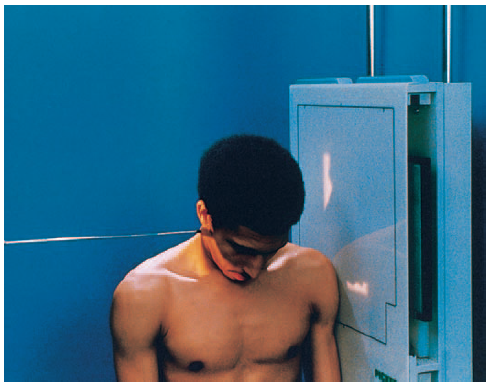
\includegraphics[width=0.7\linewidth]{imagenes/col10}
		\caption{}
		\label{fig:col10}
	\end{figure}
	
	
	\paragraph{Región de interés}
	El paciente se acerca pegado al RI para que el hombro se apoye en él. Para la hiperflexión se le indica que lleve el mentón hacia el pecho, intentando tocarse el esternón con la barbilla, manteniendo hombros y espalda quietos. No se permite que dé un paso hacia adelante. Esto sitúa las vértebras cervicales en flexión forzada para la primera exposición.
	
	\paragraph{Rayo Central}
	Horizontal, perpendicular al plano del receptor, sin angulación. Punto de entrada: \textbf{C4 (nuez de Adán)}.
	
	\paragraph{Receptor de imagen}
	Centrado a la altura de C4. El borde superior del RI se ubica aproximadamente 5 cm por encima del conducto auditivo externo (CAE). Se colima a los cuatro lados del área de interés. Deben incluirse las vértebras cervicales superiores e inferiores (C1--C7), con especial atención a C7 en hiperflexión, así como las articulaciones interapofisarias y los discos intervertebrales.
	
	\paragraph{Respiración}
	Suspendida en espiración completa: el paciente expulsa todo el aire y mantiene la apnea durante la exposición. El descenso natural de los hombros en espiración favorece la inclusión de C7.
	
	\subsubsection*{4. Anatomía Visible}
	
	Las siete vértebras cervicales (C1--C7) en posición lateral verdadera, con los cuerpos vertebrales y las apófisis espinosas de perfil. Discos intervertebrales y espacios interapofisarios. Articulaciones interapofisarias (carillas articulares) visibles como una única línea continua. Tejidos blandos anteriores: vías aéreas y laringe. En hiperflexión: los cuerpos vertebrales se juntan y las apófisis espinosas se separan (mayor apertura del espacio interespinoso). El cuerpo de la mandíbula adopta una posición casi vertical.
	
	\subsubsection*{5. Criterios de Evaluación}
	
	\textbf{Posicionamiento correcto:} Cuerpo de la mandíbula casi vertical. Las siete apófisis espinosas de perfil. Las siete vértebras cervicales en posición lateral verdadera. Se valora el grado de separación de las apófisis espinosas adyacentes: en hiperflexión normal, dichas apófisis se separan y se alejan de los cuerpos vertebrales.
	
	\textbf{Ausencia de rotación:} Las ramas mandibulares deben aparecer superpuestas entre sí. Si están desfasadas, el paciente presenta rotación: se corrige colocando el PMS paralelo al RI y asegurando que los hombros queden en un mismo plano apoyados sobre el RI. Las articulaciones interapofisarias deben verse como una única línea; si se ven dobles, indica rotación del cuello.
	
	\textbf{Penetración y contraste:} Técnica de escala larga con suficiente kVp que permita ver simultáneamente los tejidos blandos (vías aéreas, laringe) y el detalle óseo (trabeculado, cortical) junto con los espacios intervertebrales en una sola imagen.
	
	\subsubsection*{6. Puntos Críticos}
	
	\textbf{Rotación del paciente:} Las ramas mandibulares aparecen desfasadas y las carillas articulares se ven dobles. Corrección: colocar el PMS estrictamente paralelo al RI y los hombros en un mismo plano apoyados sobre el receptor.
	
	\textbf{Exclusión de C7:} La vértebra C7 queda fuera del campo por descenso insuficiente del hombro o centrado inadecuado. Corrección: pedir espiración completa para descenso natural de hombros; aumentar la DFRI; verificar centrado y campo colimado.
	
	\textbf{Adaptaciones:} No realizar proyecciones funcionales en pacientes con fractura cervical conocida o sospechada. En pacientes con movilidad reducida, registrar el máximo rango alcanzable sin forzar el movimiento.
	
	\textbf{Trucos:} Indicar claramente al paciente que no dé un paso hacia adelante al flexionar, ya que el movimiento del tronco invalida la posición lateral verdadera. La apnea en espiración, además de evitar borrosidad cinética, baja naturalmente los hombros y mejora la visualización de C7.
	
	\onecolumn
	\clearpage
	
	\begin{figure}
		\centering
		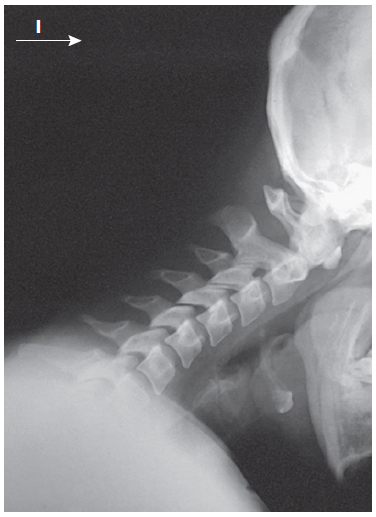
\includegraphics[width=0.7\linewidth]{imagenes/col12}
		\caption{}
		\label{fig:col12}
	\end{figure}
	
	
	\twocolumn
	\clearpage
	
	%----------------------------------------------------------
	%  Para agregar otro enfoque duplicá el bloque
	%  desde \subsection hasta \textbf{Trucos}
	%----------------------------------------------------------
	
	\subsection{Proyección Funcional - Hiperextensión}
	
	\subsubsection*{1. Identificación}
	
	\textbf{Tipo:} Proyección complementaria. Forma par con la proyección funcional de hiperflexión; ambas deben realizarse juntas como par radiológico. Si el paciente no cuenta con una de las dos, se efectúa el par completo.
	
	\textbf{Indicaciones clínicas principales:}
	\begin{itemize}
		\item Espondilolistesis (desplazamiento de una vértebra sobre otra).
		\item Latigazo cervical agudo o crónico por accidente de tránsito (evaluación de limitación del movimiento por lesión mecánica).
		\item Evaluación preoperatoria por artritis cervical.
		\item Seguimiento de artrodesis (placa, tornillos).
		\item Demostración del movimiento anteroposterior normal o de la ausencia de movimiento por traumatismo o patología; inestabilidad cervical y subluxaciones ocultas.
	\end{itemize}
	
	\subsubsection*{2. Técnica Base}
	
	\textbf{Receptor de imagen:} 24$\times$30 cm (puede usarse 18$\times$24 cm). Orientación \textbf{longitudinal}; en la práctica, a veces transversal para no cortar la apófisis espinosa de C7.
	
	\textbf{DFRI:} 140--150 cm (bibliografía: 152--183 cm). La distancia aumentada compensa la magnificación generada por la mayor distancia objeto--receptor debida al hombro que se interpone entre la columna y el RI. Una distancia mayor también contribuye a visualizar C7.
	
	\textbf{Técnica:} Homogenizada, escala larga (suficiente kVp). Permite visualizar simultáneamente el tejido blando (vías aéreas, laringe), el detalle óseo (trabeculado y cortical) y los espacios intervertebrales en una sola imagen. \textbf{kVp --- mAs}
	
	\textbf{Bucky:} Bucky de pared con grilla.
	
	\subsubsection*{3. Posicionamiento}
	
	\paragraph{Paciente}
	De pie o sentado en posición lateral verdadera. El plano medio sagital (PMS) paralelo al RI. Los hombros en un mismo plano, apoyados sobre el RI.
	
	\begin{figure}[h]
		\centering
		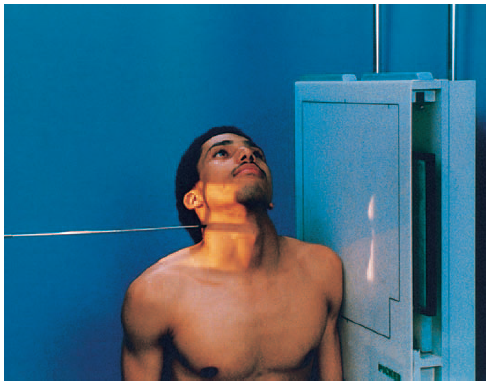
\includegraphics[width=0.7\linewidth]{imagenes/col11}
		\caption{}
		\label{fig:col11}
	\end{figure}
	
	
	\paragraph{Región de interés}
	El paciente se acerca pegado al RI para que el hombro se apoye en él. Para la hiperextensión se le indica que eleve la barbilla y deje caer la cabeza hacia atrás lo máximo que pueda (como si quisiera mirar el techo detrás suyo), manteniendo hombros y espalda quietos. No se permite que dé un paso hacia atrás. Esto sitúa las vértebras cervicales en extensión forzada para la segunda exposición.
	
	\paragraph{Rayo Central}
	Horizontal, perpendicular al plano del receptor, sin angulación. Punto de entrada: \textbf{C4 (nuez de Adán)}.
	
	\paragraph{Receptor de imagen}
	Centrado a la altura de C4. El borde superior del RI se ubica aproximadamente 5 cm por encima del conducto auditivo externo (CAE). Se colima a los cuatro lados del área de interés. Deben incluirse C1--C7, las articulaciones interapofisarias y los discos intervertebrales.
	
	\paragraph{Respiración}
	Suspendida en espiración completa: el paciente expulsa todo el aire y mantiene la apnea durante la exposición. El descenso natural de los hombros en espiración favorece la inclusión de C7.
	
	\subsubsection*{4. Anatomía Visible}
	
	Las siete vértebras cervicales (C1--C7) en posición lateral verdadera, con los cuerpos vertebrales y las apófisis espinosas de perfil. Discos intervertebrales y espacios interapofisarios. Articulaciones interapofisarias (carillas articulares) visibles como una única línea continua. Tejidos blandos anteriores: vías aéreas y laringe. En hiperextensión: los cuerpos vertebrales se separan y las apófisis espinosas se juntan (mayor cierre del espacio interespinoso). El cuerpo de la mandíbula adopta una posición casi horizontal.
	
	\subsubsection*{5. Criterios de Evaluación}
	
	\textbf{Posicionamiento correcto:} Cuerpo de la mandíbula casi horizontal. Las siete vértebras cervicales en posición lateral verdadera. Se valora el grado de separación de los cuerpos vertebrales adyacentes: en hiperextensión normal, los cuerpos se separan mientras las apófisis espinosas se aproximan.
	
	\textbf{Ausencia de rotación:} Las ramas mandibulares deben aparecer superpuestas entre sí. Si están desfasadas, el paciente presenta rotación: se corrige colocando el PMS paralelo al RI y asegurando que los hombros queden en un mismo plano apoyados sobre el RI. Las articulaciones interapofisarias deben verse como una única línea; si se ven dobles, indica rotación del cuello.
	
	\textbf{Penetración y contraste:} Técnica de escala larga con suficiente kVp que permita ver simultáneamente los tejidos blandos (vías aéreas, laringe) y el detalle óseo (trabeculado, cortical) junto con los espacios intervertebrales en una sola imagen.
	
	\subsubsection*{6. Puntos Críticos}
	
	\textbf{Rotación del paciente:} Las ramas mandibulares aparecen desfasadas y las carillas articulares se ven dobles. Corrección: colocar el PMS estrictamente paralelo al RI y los hombros en un mismo plano apoyados sobre el receptor.
	
	\textbf{Exclusión de C7:} La vértebra C7 queda fuera del campo por descenso insuficiente del hombro o centrado inadecuado. Corrección: pedir espiración completa para descenso natural de hombros; aumentar la DFRI; verificar centrado y campo colimado.
	
	\textbf{Adaptaciones:} No realizar proyecciones funcionales en pacientes con fractura cervical conocida o sospechada. En pacientes con movilidad reducida, registrar el máximo rango alcanzable sin forzar el movimiento.
	
	\textbf{Trucos:} Indicar claramente al paciente que no dé un paso hacia atrás al extender, ya que el movimiento del tronco invalida la posición lateral verdadera. La descripción ``como si quisieras mirar el techo detrás tuyo'' resulta útil para que el paciente comprenda el grado de extensión requerido.
	
	
	\onecolumn
	\clearpage
	
	\begin{figure}
		\centering
		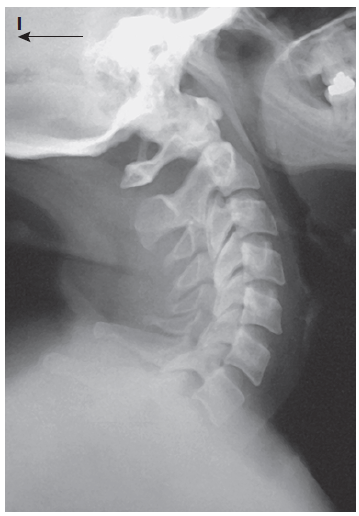
\includegraphics[width=0.7\linewidth]{imagenes/col13}
		\caption{}
		\label{fig:col13}
	\end{figure}
	
	\twocolumn
	\clearpage
	%----------------------------------------------------------
	%  Para agregar otro enfoque duplicá el bloque
	%  desde \subsection hasta \textbf{Trucos}
	%----------------------------------------------------------
	
	
%%%%%%%%%%%%%%%%%%%%%%%%%%%%%%%%%%%%%%%%%%%%%%%%%%%%%%%%%%%
%  SECCIÓN: Columna Cervical
%  Archivo: secciones/columna_cervical.tex
%  Sin preámbulo ni \begin{document} — lo maneja main.tex
	%%%%%%%%%%%%%%%%%%%%%%%%%%%%%%%%%%%%%%%%%%%%%%%%%%%%%%%%%%%
	
	\section{Columna Cervical}
	
	\subsection{Oblicua Posterior Derecha (OPD) - Oblicua Posterior Izquierda (ODI) - AP}
	
	\subsubsection*{1. Identificación}
	
	\textbf{Tipo:} Proyección complementaria. Forma par con la proyección oblicua contralateral (OPD con ODI y viceversa); siempre se realizan en conjunto.
	
	\textbf{Indicaciones clínicas principales:}
	\begin{itemize}
		\item Estenosis cervical de los orificios intervertebrales (compresión del canal espinal y raíces nerviosas)
		\item Osteofitosis y discopatías cervicales
		\item Cervicobraquialgia, radiculopatía y parestesias (dolor al flexionar el cuello o adormecimiento de manos)
	\end{itemize}
	
	\subsubsection*{2. Técnica Base}
	
	\textbf{Receptor de imagen:} 18$\times$24 cm o 24$\times$30 cm. Orientación \textbf{longitudinal} (vertical). El RI se centra a nivel de C3, aproximadamente 2{,}5 cm por encima del punto más prominente del cartílago tiroides, para compensar la angulación craneal del rayo central.
	
	\textbf{DFRI:} 150--180 cm. La distancia mayor se emplea para compensar el aumento de OID generado por la presencia de los hombros respecto al receptor de imagen.
	
	\textbf{Técnica:} Homogeneizada (escala larga, kVp suficiente). Permite atravesar y visualizar los diferentes espesores desiguales presentes en la proyección: hombro, hueso, aire y tejido blando cervical.
	
	\textbf{Bucky:} Bucky mural o de mesa con grilla, según la posición del paciente.
	
	\subsubsection*{3. Posicionamiento}
	
	\paragraph{Paciente}
	De pie (preferido por comodidad), sentado o en decúbito semisupino con la espalda apoyada contra el receptor. Se parte de la posición AP estándar con el plano medio sagital perpendicular al RI.
	
	\begin{figure}[h]
		\centering
		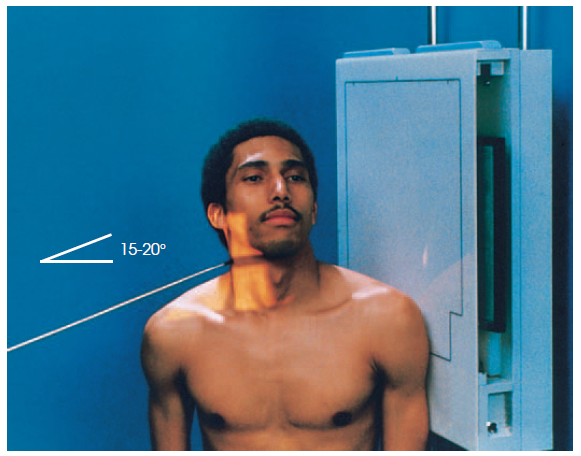
\includegraphics[width=0.7\linewidth]{imagenes/col14}
		\caption{Proyección AP axial oblicua en bipedestación de los agujeros intervertebrales derechos: posición\textbf{ OPI}.}
		\label{fig:col14}
	\end{figure}
	
	
	\paragraph{Región de interés}
	El cuerpo y la cabeza se rotan conjuntamente 45° respecto al plano del RI, apoyando la espalda contra el receptor. Se solicita al paciente que eleve y adelante el mentón para evitar superposición con las vértebras superiores, y que baje los hombros para no cubrir C7. Es fundamental que el mentón no gire hacia un lado, para evitar rotación de las primeras vértebras cervicales superiores. En posición semisupino: se colocan apoyos bajo la parte inferior del tórax y la cadera elevada, y un apoyo adicional bajo la cabeza.
	
	\paragraph{Rayo Central}
	Angulado 15--20° en dirección \textbf{craneal}, dirigido a \textbf{C4 (nuez de Adán)}. La angulación craneal responde a la orientación caudocraneal de los agujeros intervertebrales (inclinados aproximadamente 15° de atrás hacia adelante), permitiendo un paso tangencial a través de ellos y evitando que los hombros cubran C7.
	
	\paragraph{Receptor de imagen}
	Centrado a nivel de C3 (2{,}5 cm por encima del cartílago tiroides más prominente). Colimación a los bordes laterales de las partes blandas del cuello y a los bordes superior e inferior del RI. La región a incluir abarca desde la base del cráneo hasta los cuerpos vertebrales C1--C7 y T1, visualizando la transición cervicotorácica.
	
	\paragraph{Respiración}
	Suspendida al momento de la exposición. Permite eliminar el movimiento de las estructuras cervicales y garantiza nitidez en la imagen.
	
	\subsubsection*{4. Anatomía Visible}
	
	Se demuestran los agujeros intervertebrales del lado \textbf{más alejado del receptor} (C2--C3 a C7--T1) en posición abierta, permitiendo evaluar estenosis foraminal. Los pedículos del lado más alejado del RI quedan proyectados en visión de perfil. Los espacios discales intervertebrales aparecen abiertos por la curvatura cervical. Los cuerpos vertebrales se proyectan en oblicuo. El hueso occipital puede superponerse levemente a C1, lo cual es esperado y aceptable. Los hombros no deben cubrir C7.
	
	\subsubsection*{5. Criterios de Evaluación}
	
	\textbf{Posicionamiento correcto:} Agujeros intervertebrales del lado más alejado del receptor abiertos y de tamaño y contorno uniformes desde C2--C3 hasta C7--T1. Espacios discales intervertebrales abiertos. Barbilla elevada, sin superposición de la mandíbula sobre las vértebras superiores (atlas y axis). Hueso occipital superpuesto a C1 (aceptable y esperado). Hombros sin cubrir C7.
	
	\textbf{Ausencia de rotación:} Rotación homogénea de 45° del tronco y la cabeza. Si los agujeros intervertebrales aparecen cerrados, indica corrección insuficiente de la rotación del tronco. Tamaño y contorno uniformes de todos los agujeros visibles.
	
	\textbf{Penetración y contraste:} Técnica homogeneizada con escala larga (alto kVp). Debe permitir diferenciar simultáneamente los distintos espesores: tejido blando cervical, hueso, aire y región de hombros.
	
	\subsubsection*{6. Puntos Críticos}
	
	\textbf{Agujeros intervertebrales cerrados o vértebras amontonadas:} Indica insuficiente angulación craneal del RC o rotación de tronco incorrecta. Corregir aumentando la angulación craneal (hasta 20°) y verificando los 45° de rotación del cuerpo.
	
	\textbf{Mandíbula superpuesta a atlas y axis:} El mentón no fue elevado o adelantado correctamente. Solicitar al paciente que eleve y protruya el mentón. Verificar que no gire el mentón lateralmente para evitar rotación de las vértebras superiores.
	
	\textbf{Adaptaciones:} En paciente con trauma o limitación de movimiento, puede realizarse en decúbito semisupino con apoyos bajo tórax y cadera. La posición supina es equivalente en resultado si la rotación de 45° se mantiene correcta.
	
	\textbf{Trucos:} Las oblicuas cervicales posteriores se marcan como proyecciones de frente (no de perfil): la marca derecha corresponde al lado derecho de la imagen. Para identificar el lado en la radiografía, observar la posición de la mandíbula: si queda hacia la izquierda, corresponde a oblicua posterior derecha o anterior izquierda. Siempre se realizan ambas oblicuas (OPD y ODI) para comparación bilateral.
	
	
	\onecolumn
	\clearpage
	
	\begin{figure}
		\centering
		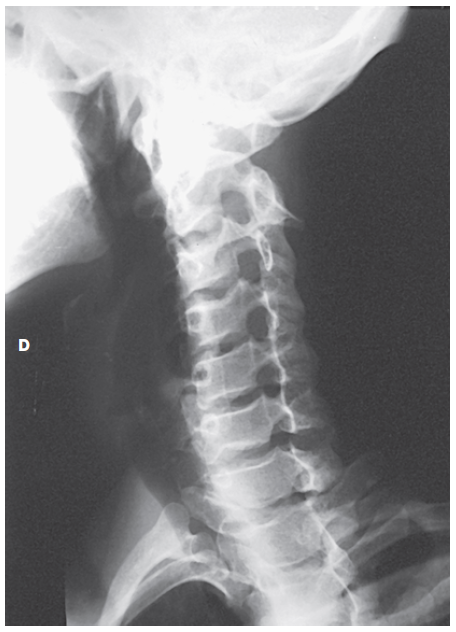
\includegraphics[width=0.7\linewidth]{imagenes/col16}
		\caption{Posición OPD para la demostración del lado izquierdo.
		}
		\label{fig:col16}
	\end{figure}
		
	
	\twocolumn
	\clearpage
	
	\onecolumn
	\clearpage
	
	\begin{figure}
		\centering
		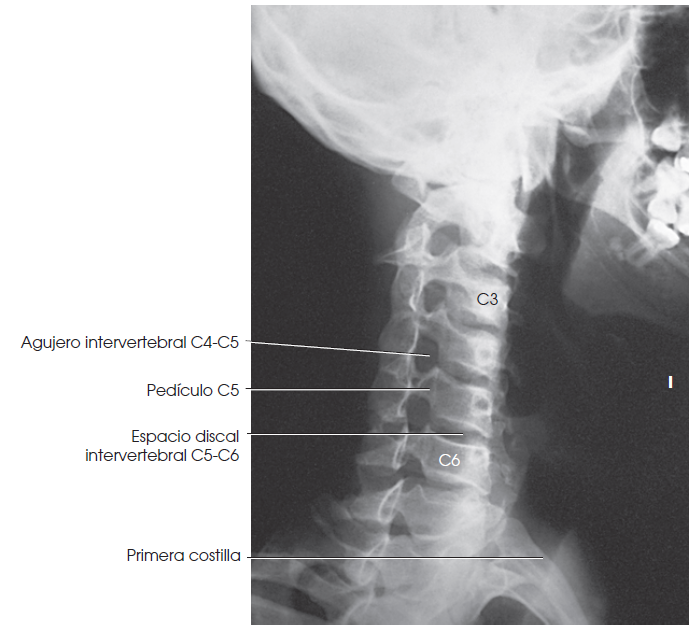
\includegraphics[width=0.7\linewidth]{imagenes/col15}
		\caption{Posición OPI para la demostración del lado derecho.
		}
		\label{fig:col15}
	\end{figure}
		
	
	\twocolumn
	\clearpage
	%----------------------------------------------------------
	%  Para agregar otro enfoque duplicá el bloque
	%  desde \subsection hasta \textbf{Trucos}
	%----------------------------------------------------------
	
	
	%%%%%%%%%%%%%%%%%%%%%%%%%%%%%%%%%%%%%%%%%%%%%%%%%%%%%%%%%%%
	%  SECCIÓN: Columna Cervical — PA Oblicuas Anteriores
	%  Archivo: secciones/oblicuas_anteriores_cervical.tex
	%  Sin preámbulo ni \begin{document} — lo maneja main.tex
		%%%%%%%%%%%%%%%%%%%%%%%%%%%%%%%%%%%%%%%%%%%%%%%%%%%%%%%%%%%
		
		\section{Columna Cervical}
		
		\subsection{Oblicua Anterior Derecha (OAD) - Oblicua Anterior Izquierda (OAI)}
		
		\subsubsection*{1. Identificación}
		
		\textbf{Tipo:} Complementaria. Forma par con las oblicuas posteriores (OPD/OPI); ambos lados se realizan siempre para comparación bilateral.
		
		\textbf{Indicaciones clínicas principales:}
		\begin{itemize}
			\item Estenosis de los orificios intervertebrales cervicales (compresión del canal espinal y raíces nerviosas)
			\item Osteofitosis y discopatías cervicales
			\item Cervicobraquialgia, radiculopatía y parestesias (dolor al flexionar el cuello o adormecimiento de manos)
		\end{itemize}
		
		\subsubsection*{2. Técnica Base}
		
		\textbf{Receptor de imagen:} 18$\times$24 cm o 24$\times$30 cm. Orientación \textbf{longitudinal}. Centrado a la altura de C5 (2,5 cm caudal al punto más prominente del cartílago tiroides).
		
		\textbf{DFRI:} 150--180 cm. La mayor distancia compensa el aumento de OID propio de la proyección oblicua y mejora la nitidez de la imagen.
		
		\textbf{Técnica:} Homogeneizada (escala larga, kVp suficiente). Permite atravesar y visualizar los diferentes espesores de la región: hombro, hueso, aire y tejido blando cervical.
		
		\textbf{Bucky:} Bucky de pared con grilla.
		
		\subsubsection*{3. Posicionamiento}
		
		\paragraph{Paciente}
		De pie o sentado en bipedestación, con el hombro apoyado contra el Bucky de pared. El paciente queda de cara al tubo (posición PA). También puede realizarse en decúbito prono (semiprono). Los brazos se mantienen a los lados del cuerpo; en espiración los hombros descienden, mejorando la visualización de C7.
		
		\begin{figure}[h]
			\centering
			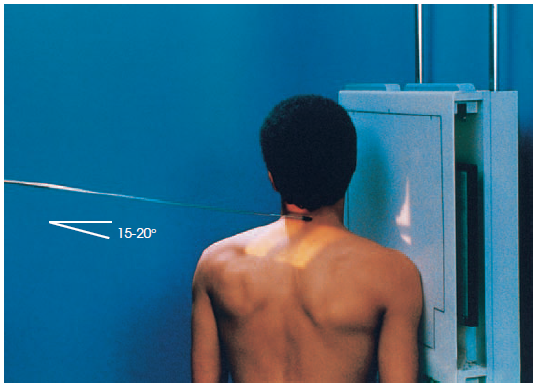
\includegraphics[width=0.7\linewidth]{imagenes/col17}
			\caption{}
			\label{fig:col17}
		\end{figure}
		
		\begin{figure}[h]
			\centering
			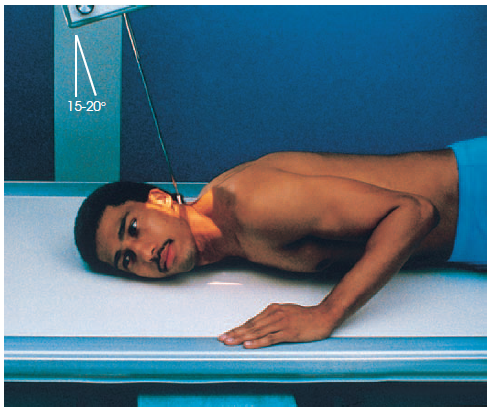
\includegraphics[width=0.7\linewidth]{imagenes/col18}
			\caption{}
			\label{fig:col18}
		\end{figure}
		
		
		
		\paragraph{Región de interés}
		Se rota todo el cuerpo del paciente 45° respecto al receptor de imagen, de modo que los agujeros intervertebrales del lado más alejado del RI queden en paralelo al plano del receptor. El plano medio sagital debe quedar alineado con el eje de la columna. Se eleva y hace protruir la barbilla lo suficiente para evitar la superposición de la mandíbula sobre las vértebras cervicales superiores (atlas y axis). En posición semiprono se utiliza el antebrazo y la rodilla flexionada del lado elevado como apoyo.
		
		\paragraph{Rayo Central}
		Angulado \textbf{15--20° en dirección caudal}, dirigido hacia \textbf{C4 (nuez de Adán)}. La angulación caudal coincide con la dirección descendente de los agujeros intervertebrales vistos desde atrás, permitiendo proyectarlos abiertos.
		
		\paragraph{Receptor de imagen}
		Centrado a la altura de C5. La colimación abarca los bordes laterales de las partes blandas del cuello y los bordes superior e inferior coinciden con los bordes del RI. La región a incluir es desde la base del cráneo hasta T1.
		
		\paragraph{Respiración}
		Suspendida en espiración. La espiración favorece el descenso de los hombros, liberando la visualización de C7 y reduciendo la necesidad de aumentar la angulación.
		
		\subsubsection*{4. Anatomía Visible}
		
		Agujeros intervertebrales del lado \textbf{más alejado del RI} (los más próximos al tubo), desde C2--C3 hasta C7--T1, proyectados abiertos. Pedículos del lado más cercano al receptor. Cuerpos vertebrales cervicales en proyección oblicua con espacios interdiscales abiertos. Articulaciones uncovertebrales. La mandíbula no debe superponerse al atlas ni al axis; el hueso occipital no debe superponerse al axis; los hombros no deben tapar C7.
		
		\subsubsection*{5. Criterios de Evaluación}
		
		\textbf{Posicionamiento correcto:} Agujeros intervertebrales del lado alejado al RI abiertos y de tamaño y contorno uniformes desde C2 hasta C7--T1. Espacios interdiscales abiertos. Barbilla elevada sin superposición mandibular sobre vértebras superiores. Todas las vértebras cervicales incluidas hasta T1.
		
		\textbf{Ausencia de rotación:} Rotación corporal exacta de 45°; si los agujeros aparecen cerrados, la rotación del tronco es insuficiente o excesiva y debe corregirse.
		
		\textbf{Penetración y contraste:} Técnica homogeneizada que permite diferenciar simultáneamente el hombro, el hueso, el aire y el tejido blando cervical en una escala de grises larga.
		
		\subsubsection*{6. Puntos Críticos}
		
		\textbf{Agujeros intervertebrales cerrados:} Indica rotación corporal inadecuada (diferente a 45°). Corregir la rotación del tronco hasta lograr el ángulo exacto.
		
		\textbf{Superposición mandibular sobre vértebras superiores:} La barbilla no fue elevada ni protraída suficientemente. Indicar al paciente que eleve y adelante el mentón.
		
		\textbf{Adaptaciones:} Si los hombros tapan C7, aumentar la angulación caudal o indicar al paciente que baje activamente los hombros. En pacientes con limitación de movilidad puede realizarse en decúbito semiprono usando antebrazo y rodilla como apoyo.
		
		\textbf{Trucos:} La angulación es caudal (opuesta a las oblicuas posteriores AP). Se prefieren las oblicuas anteriores sobre las posteriores por la menor dosis de radiación a la tiroides (tiroides queda en RP). Para identificar la proyección en la radiografía: si el mentón apunta hacia la marca derecha es OAI u OPD; si apunta hacia la marca izquierda es OAD u OPI. Las oblicuas anteriores demuestran los agujeros del lado \textbf{más alejado} del receptor (a diferencia de las posteriores, que muestran los más cercanos).
		
		\onecolumn
		\clearpage
		
		\begin{figure}
			\centering
			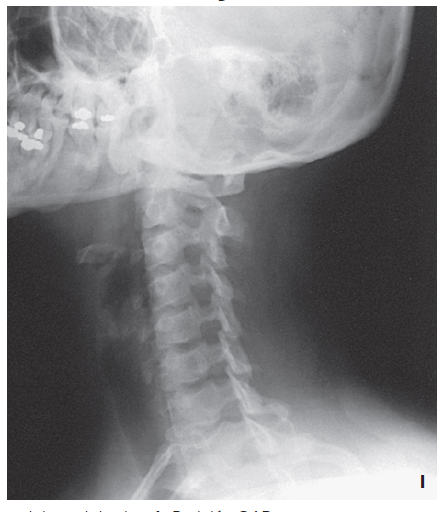
\includegraphics[width=0.7\linewidth]{imagenes/col20}
			\caption{Posición OAI para la demostración del lado izquierdo.
			}
			\label{fig:col20}
		\end{figure}
		
		
		\twocolumn
		\clearpage
		
		
		\onecolumn
		\clearpage
		
		\begin{figure}
			\centering
			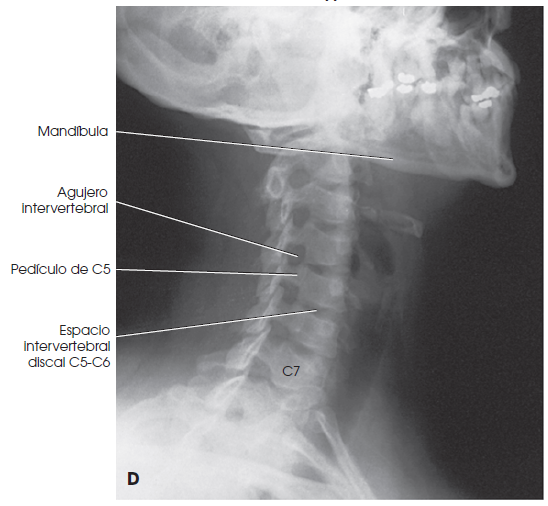
\includegraphics[width=0.7\linewidth]{imagenes/col19}
			\caption{Posición OAD para la demostración del lado derecho.}
			\label{fig:col19}
		\end{figure}
		
		
		\twocolumn
		\clearpage
		
		
		%----------------------------------------------------------
		%  Para agregar otro enfoque duplicá el bloque
		%  desde \subsection hasta \textbf{Trucos}
		%----------------------------------------------------------
		
		
		
	%%%%%%%%%%%%%%%%%%%%%%%%%%%%%%%%%%%%%%%%%%%%%%%%%%%%%%%%%%%
	%  SECCIÓN: Columna Torácica
	%  Archivo: secciones/pasaje_cervico_dorsal.tex
	%  Sin preámbulo ni \begin{document} — lo maneja main.tex
		%%%%%%%%%%%%%%%%%%%%%%%%%%%%%%%%%%%%%%%%%%%%%%%%%%%%%%%%%%%
		
		\section{Columna Torácica}
		
		\subsection{Pasaje Cérvico-Dorsal - Técnica del Nadador (Método de Twining)}
		
		\subsubsection*{1. Identificación}
		
		\textbf{Tipo:} Proyección complementaria. Forma par con la proyección lateral de columna torácica.
		
		\textbf{Indicaciones clínicas principales:}
		\begin{itemize}
			\item Traumatismo cervical, fractura o luxación de C7 o T1.
			\item Cervicobraquialgia: dolor irradiado a los brazos y la base del cuello.
			\item Cuello rígido.
			\item Proyección de elección cuando los hombros prominentes ocultan C7--T1 en la lateral cervical estándar, impidiendo la visualización de la cabeza del húmero.
			\item Proyección lateral de vértebras torácicas superiores y región de transición C7--T1.
		\end{itemize}
		
		\subsubsection*{2. Técnica Base}
		
		\textbf{Receptor de imagen:} 24x30 cm. Orientación \textbf{longitudinal} (vertical), centrado a la altura del espacio C7--T1, localizado 5 cm por encima de la escotadura yugular. \textbf{Filtro de compensación obligatorio:} las diferencias extremas de densidad entre el cuello fino y la región torácica gruesa exigen el uso de un filtro especialmente diseñado para demostrar el área C7--T1 en una sola imagen.
		
		\textbf{DFRI:} 150 o 180 cm. La mayor distancia reduce la penumbra geométrica y minimiza la magnificación de estructuras profundas en esta región anatómicamente compleja.
		
		\textbf{Técnica:} Intermedia. Se utiliza un kVp suficiente para atravesar el hombro y un mAs elevado para ganar densidad en los cuerpos vertebrales sin sobreexponer el aire del cuello. Los valores dependen del biotipo del paciente. Técnica respiratoria opcional: bajo mAs con tiempo de exposición de 3--4 segundos, solicitando al paciente respiraciones breves y regulares para difuminar la anatomía pulmonar y mejorar la visualización ósea.
		
		\textbf{Bucky:} Sí, con grilla. El uso de grilla es necesario dada la cantidad de tejido atravesado en la región del hombro y la parte superior del tórax.
		
		\subsubsection*{3. Posicionamiento}
		
		\paragraph{Paciente}
		El paciente se coloca en posición lateral verdadera, de pie (preferible), sentado o en decúbito lateral. El plano medio sagital debe quedar paralelo al plano del RI. En decúbito lateral, la cabeza se eleva sobre el brazo del paciente o un soporte firme; puede colocarse un apoyo bajo la parte inferior del tórax para alinear la columna. Si el paciente está incorporado, se apoya en un dispositivo de rejilla vertical.
		
		\begin{figure}[h]
			\centering
			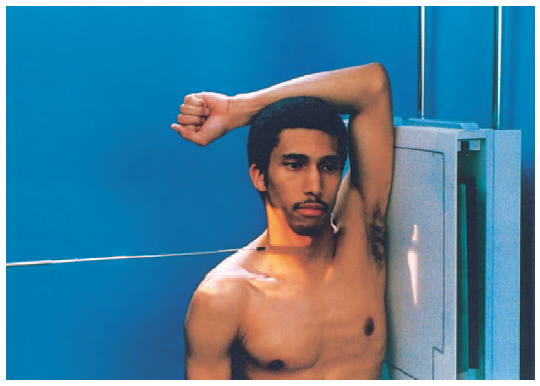
\includegraphics[width=0.7\linewidth]{imagenes/col21}
			\caption{}
			\label{fig:col21}
		\end{figure}
		
		\begin{figure}[h]
			\centering
			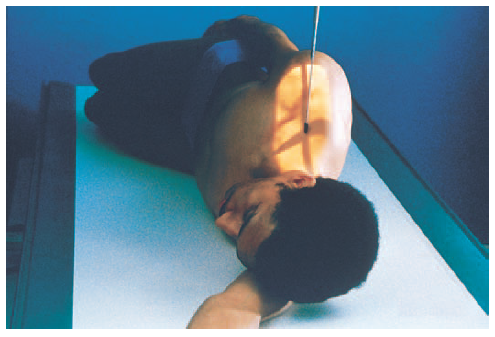
\includegraphics[width=0.7\linewidth]{imagenes/col22}
			\caption{}
			\label{fig:col22}
		\end{figure}
		
		
		
		\paragraph{Región de interés}
		El plano medio coronal del cuerpo se centra en la línea media de la rejilla. El brazo próximo al RI se extiende por encima de la cabeza desplazando la cabeza humeral hacia anterior (recomendado) para que no se superponga a la columna dorsal. Si el paciente está incorporado, el codo se flexiona y el antebrazo se apoya sobre la cabeza. El brazo alejado del RI se desciende lo máximo posible a lo largo del cuerpo, traccionándolo hacia posterior para separar ambos hombros en sentido vertical. Con estos dos movimientos se liberan las cabezas humerales y la columna cérvico-dorsal queda sin superposición. Se recomienda una leve rotación del paciente hacia anterior junto con el brazo elevado para terminar de separar las estructuras.
		
		\paragraph{Rayo Central}
		Perpendicular al plano del receptor, dirigido al espacio C7--T1, localizado \textbf{5 cm por encima de la escotadura yugular}. Si el paciente no puede descender el hombro alejado del RI, se aplica una angulación \textbf{caudal de 3--5°} para compensar la diferencia de altura entre los hombros.
		
		\paragraph{Receptor de imagen}
		Centrado a la altura del espacio C7--T1. La región de inclusión debe abarcar superiormente desde C4--C5 e inferiormente hasta T3--T4 para asegurar la visualización completa de la transición cérvico-torácica, incluyendo cuerpos vertebrales y apófisis espinosas. Siempre debe visualizarse el pasaje de una región a otra (C7--T1).
		
		\paragraph{Respiración}
		Suspendida en espiración. Si el paciente coopera, puede utilizarse la \textbf{técnica respiratoria opcional}: se solicitan respiraciones breves y regulares durante un tiempo de exposición de 3--4 segundos con bajo mAs, lo que difumina la anatomía pulmonar y resalta las estructuras óseas vertebrales.
		
		\subsubsection*{4. Anatomía Visible}
		
		Se visualizan las vértebras cervicales inferiores y las vértebras torácicas superiores entre los hombros. La región de transición cérvico-torácica (C7--T1) debe quedar claramente demostrada. Los cuerpos vertebrales y las apófisis espinosas deben incluirse en el campo. La separación de las cabezas humerales mediante la posición diferencial de los brazos permite liberar la columna de superposiciones. Los agujeros intervertebrales torácicos se visualizan en perfil sin necesidad de enfoques específicos, dado que se ubican a 45° respecto al plano sagital y en posición lateral ya se proyectan adecuadamente.
		
		\subsubsection*{5. Criterios de Evaluación}
		
		\textbf{Posicionamiento correcto:} Vértebras cervicales inferiores y torácicas superiores visibles entre los hombros, sin rotación significativa respecto a una posición lateral verdadera. El espacio C7--T1 debe estar centrado en la imagen. La región incluye desde C4--C5 hasta T3--T4, con cuerpos vertebrales y apófisis espinosas presentes.
		
		\textbf{Ausencia de rotación:} Cuerpos vertebrales de perfil, sin doble contorno. Si presentan doble contorno, el PMS no está paralelo al RI y debe corregirse. Las cabezas humerales deben estar mínimamente superpuestas a la columna vertebral. En posición lateral estricta la cabeza humeral tiende a superponerse al pasaje cérvico-dorsal; debe evitarse mediante la separación diferencial de los brazos.
		
		\textbf{Penetración y contraste:} Adecuada penetración de los rayos X a través de la región del hombro, con densidad suficiente para visualizar los cuerpos vertebrales sin sobreexponer el aire del cuello. El filtro de compensación debe haber equilibrado la diferencia de densidades entre el cuello y la región torácica superior, produciendo una imagen de densidad uniforme en toda la columna estudiada.
		
		\subsubsection*{6. Puntos Críticos}
		
		\textbf{Superposición humeral sobre la columna:} Si las cabezas humerales se superponen al espacio C7--T1, la proyección pierde su utilidad diagnóstica. Corrección: asegurar la máxima separación vertical de los hombros mediante la extensión del brazo proximal sobre la cabeza y el descenso del brazo distal; aplicar leve rotación anterior del brazo elevado.
		
		\textbf{Diferencia extrema de densidades:} Sin filtro de compensación, el cuello queda sobreexpuesto y la región torácica subexpuesta en la misma imagen, impidiendo la evaluación de C7--T1. Corrección: el uso del filtro de compensación es obligatorio en esta proyección.
		
		\textbf{Adaptaciones:} Si el paciente no puede descender el hombro alejado del RI, angular el RC caudal 3--5° incidiendo en C7--T1. Si en la imagen obtenida la cabeza humeral queda superpuesta al pasaje cérvico-dorsal por no haber oblicuado el brazo elevado ni movilizado el hombro contralateral, repetir la proyección corrigiendo el posicionamiento o angulando el RC. En decúbito lateral, colocar apoyo bajo el tórax inferior para alinear la columna con el RI.
		
		\textbf{Trucos:} La técnica respiratoria (3--4 segundos, respiraciones breves regulares) es especialmente útil para difuminar estructuras pulmonares y mejorar la nitidez ósea vertebral. La recomendación de desplazar el húmero del brazo elevado hacia anterior evita que se proyecte sobre la columna dorsal. Siempre verificar que el pasaje C7--T1 quede incluido y visible, ya que es el objetivo diagnóstico central de esta proyección.
		
		
		
		\clearpage
		\onecolumn
		
		\begin{figure}
			\centering
			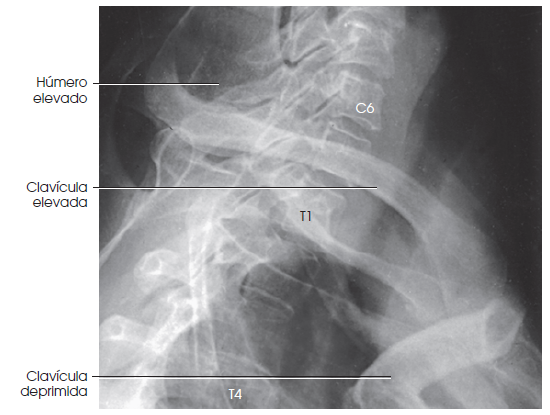
\includegraphics[width=0.7\linewidth]{imagenes/col23}
			\caption{}
			\label{fig:col23}
		\end{figure}
		
		
		\twocolumn
		\clearpage
		%----------------------------------------------------------
		%  Para agregar otro enfoque duplicá el bloque
		%  desde \subsection hasta \textbf{Trucos}
		%----------------------------------------------------------
		
		
	%%%%%%%%%%%%%%%%%%%%%%%%%%%%%%%%%%%%%%%%%%%%%%%%%%%%%%%%%%%
	%  SECCIÓN: Columna Dorsal
	%  Archivo: secciones/columna_dorsal.tex
	%  Sin preámbulo ni \begin{document} — lo maneja main.tex
		%%%%%%%%%%%%%%%%%%%%%%%%%%%%%%%%%%%%%%%%%%%%%%%%%%%%%%%%%%%
		
		\section{Columna Torácica}
		
		\subsection{Frente de Columna Torácica}
		
		\subsubsection*{1. Identificación}
		
		\textbf{Tipo:} Proyección básica. Forma par con la proyección lateral de columna dorsal.
		
		\textbf{Indicaciones clínicas principales:}
		\begin{itemize}
			\item Dorsalgia crónica
			\item Cifosis (joroba)
			\item Fracturas por compresión
			\item Escoliosis
		\end{itemize}
		
		\subsubsection*{2. Técnica Base}
		
		\textbf{Receptor de imagen:} 35$\times$43 cm. Orientación \textbf{longitudinal}. Borde superior del RI ubicado 4 a 5 cm por encima de los hombros, de forma que se incluya el pasaje C7-T1 en el extremo superior y el pasaje T12-L1 en el extremo inferior, permitiendo contar e identificar cada vértebra.
		
		\textbf{DFRI:} 100 cm.
		
		\textbf{Técnica:} Homogeneizada (alto kVp). Se utiliza alto kVp para engreír las distintas densidades y poder atravesar todo el espesor de la región, compensando la diferencia de grosor entre el extremo superior (tórax) y el extremo inferior (abdomen superior). Se orienta el ánodo hacia la cabeza y el cátodo hacia los pies, aprovechando que el cátodo emite mayor intensidad de rayos para atravesar la zona de mayor densidad.
		
		\textbf{Bucky:} Bucky de mesa o de pared. Grilla sí.
		
		\subsubsection*{3. Posicionamiento}
		
		\paragraph{Paciente}
		Decúbito supino (sin almohada para no acentuar la cifosis torácica) o en bipedestación. El plano medio sagital debe quedar perpendicular al receptor de imagen. En posición supina, se flexionan caderas y rodillas con los muslos en posición vertical para reducir la cifosis torácica y lograr un contacto más uniforme de la columna con el receptor. Los brazos se disponen a los lados del cuerpo y los hombros deben encontrarse en un mismo plano.
		
		\begin{figure}[h]
			\centering
			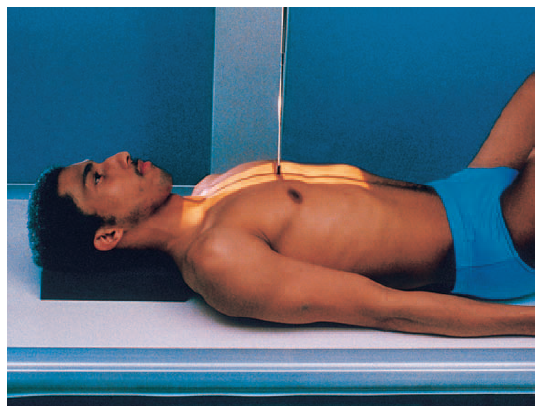
\includegraphics[width=0.7\linewidth]{imagenes/col25}
			\caption{}
			\label{fig:col25}
		\end{figure}
		
		
		\paragraph{Región de interés}
		Columna alineada y centrada en la porción media del receptor. Los hombros deben estar en un mismo plano, sin rotación del tronco, de modo que el plano medio sagital quede perpendicular al RI.
		
		\paragraph{Rayo Central}
		Perpendicular al plano del receptor. Punto de entrada: \textbf{T6}, que se localiza en el punto medio entre la escotadura yugular (T3) y el apéndice xifoides (T9), aproximadamente una palma de ancho hacia cada lado. Colimar estrechamente sobre la columna torácica.
		
		\paragraph{Receptor de imagen}
		Centrado en D6. Borde superior 4 a 5 cm por encima de los hombros para asegurar la inclusión del pasaje C7-D1 superiormente y del pasaje T12-L1 inferiormente.
		
		\paragraph{Respiración}
		Suspendida al final de una espiración forzada. Al espirar, el diafragma asciende, logrando una densidad más uniforme que facilita la visualización de las vértebras inferiores (T9-T12), que de otro modo quedarían ocultas por la sombra diafragmática.
		
		\subsubsection*{4. Anatomía Visible}
		
		Se deben visualizar las 12 vértebras torácicas en su totalidad, incluyendo los cuerpos vertebrales, apófisis espinosas, pedículos y costillas articuladas. Se debe incluir el pasaje cérvico-dorsal (C7-T1) y el pasaje dorso-lumbar (T12-L1), imprescindibles para la identificación y conteo correcto de cada vértebra. Con receptor de 35$\times$43 cm también deben visualizarse las columnas laterales, los hombros, los campos pulmonares y el diafragma. La identificación se realiza buscando la primera vértebra que porta costilla (T1) desde arriba y verificando que la última vértebra visible también las posea (T12); puede haber excepciones por costillas o vértebras supernumerarias, que se identifican por ser de menor tamaño o no coincidir con el conteo habitual.
		
		\subsubsection*{5. Criterios de Evaluación}
		
		\textbf{Posicionamiento correcto:} Las 12 vértebras torácicas deben estar visibles con densidad uniforme. Si no es posible lograr densidad uniforme en una sola toma, se obtienen dos radiografías separadas: una para vértebras superiores y otra para las inferiores. La columna vertebral debe estar alineada en la línea media de la radiografía. El haz debe estar colimado sobre la columna torácica.
		
		\textbf{Ausencia de rotación:} Las articulaciones esterno claviculares deben estar equidistantes respecto a la línea media de la columna. Las apófisis espinosas deben estar centradas en los cuerpos vertebrales. Si las espinosas aparecen desviadas, el paciente está rotado: corregir colocando el plano medio sagital perpendicular al RI.
		
		\textbf{Penetración y contraste:} La técnica homogeneizada de alto kVp debe mostrar densidad uniforme a lo largo de toda la columna, permitiendo visualizar tanto las vértebras superiores (menor espesor) como las inferiores (mayor espesor abdominal) en una sola imagen.
		
		\subsubsection*{6. Puntos Críticos}
		
		\textbf{Rotación del paciente:} Las apófisis espinosas aparecen desviadas del centro de los cuerpos vertebrales y las articulaciones esterno claviculares pierden su equidistancia. Corregir asegurando que el plano medio sagital quede estrictamente perpendicular al RI.
		
		\textbf{Cifosis no compensada:} Si no se flexionan caderas y rodillas en decúbito supino, la cifosis torácica acentuada aleja parte de la columna del receptor, aumentando el OID y degradando la nitidez. Corregir flexionando caderas y rodillas o utilizando la posición en bipedestación.
		
		\textbf{Adaptaciones:} En pacientes con cifosis severa o en trauma, puede utilizarse la posición en bipedestación o con apoyo adicional. En pacientes con diferencia de grosor muy marcada puede requerirse el uso de filtro de compensación o dos exposiciones separadas.
		
		\textbf{Trucos:} Orientar el cátodo hacia los pies (zona de mayor densidad del abdomen superior) aprovecha el efecto de talón del ánodo para lograr mayor intensidad donde más se necesita. La espiración forzada eleva el diafragma y homogeneiza la densidad de las vértebras inferiores. Para contar vértebras, identificar T1 como la primera con costilla desde arriba y verificar que T12 sea la última con costilla hacia abajo.
		
		
		\onecolumn
		\clearpage
		
		\begin{figure}
			\centering
			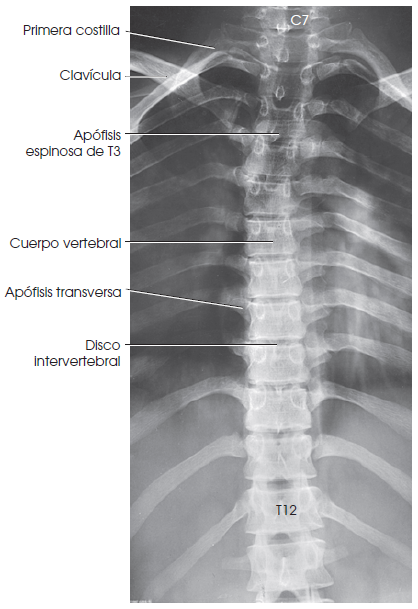
\includegraphics[width=0.7\linewidth]{imagenes/col24}
			\caption{El extremo catódico (-) del tubo de rayos X sobre la parte inferior del tórax (una densidad más uniforme).
			}
			\label{fig:col24}
		\end{figure}
		
		
		\twocolumn
		\clearpage
		
		%----------------------------------------------------------
		%  Para agregar otro enfoque duplicá el bloque
		%  desde \subsection hasta \textbf{Trucos}
		%----------------------------------------------------------
		
		
	%%%%%%%%%%%%%%%%%%%%%%%%%%%%%%%%%%%%%%%%%%%%%%%%%%%%%%%%%%%
	%  SECCIÓN: Columna Torácica
	%  Archivo: secciones/columna_toracica.tex
	%  Sin preámbulo ni \begin{document} — lo maneja main.tex
		%%%%%%%%%%%%%%%%%%%%%%%%%%%%%%%%%%%%%%%%%%%%%%%%%%%%%%%%%%%
		
		\section{Columna Torácica}
		
		\subsection{Lateral de Columna Torácica (Perfil)}
		
		\subsubsection*{1. Identificación}
		
		\textbf{Tipo:} Proyección complementaria. Forma par con la proyección AP de columna torácica.
		
		\textbf{Indicaciones clínicas principales:}
		\begin{itemize}
			\item Fracturas por compresión vertebral
			\item Subluxación vertebral
			\item Cifosis
		\end{itemize}
		
		\subsubsection*{2. Técnica Base}
		
		\textbf{Receptor de imagen:} 35$\times$43 cm. Orientación \textbf{longitudinal}. El borde superior del RI se ubica 4--5 cm por encima de los hombros.
		
		\textbf{DFRI:} 100 cm.
		
		\textbf{Técnica:} Técnica homogenizada (técnica respiratoria). Se separa el miliamperaje de los segundos; se aumenta el tiempo de exposición a 1400--1600 ms (equivalente a un ciclo respiratorio completo). Durante el disparo el paciente respira con normalidad (inspira y espira), lo que genera borrosidad cinética de los arcos costales, dejando la columna con mayor nitidez. La técnica respiratoria implica mayor dosis, por lo que no se indica en niños ni en pacientes con dolor agudo intenso.
		
		\textbf{Bucky:} Bucky de pared o de mesa según posición del paciente. Grilla obligatoria dada la técnica utilizada.
		
		\subsubsection*{3. Posicionamiento}
		
		\paragraph{Paciente}
		Decúbito lateral izquierdo (para que el corazón quede más próximo al RI) o en bipedestación. El paciente viste bata abierta por detrás de la columna. Se coloca almohada bajo la cabeza para mantener el eje longitudinal de la columna vertebral en posición horizontal. Se flexionan caderas y rodillas. El plano medio sagital debe mantenerse paralelo al RI.
		
		\begin{figure}[h]
			\centering
			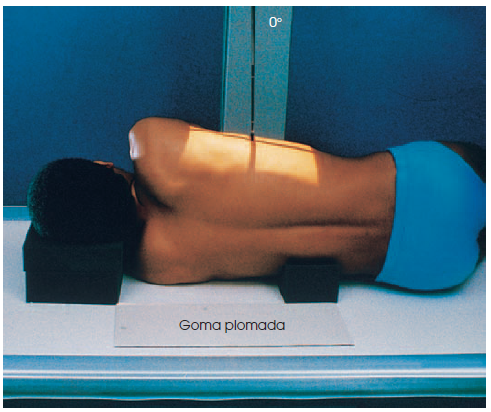
\includegraphics[width=0.7\linewidth]{imagenes/col27}
			\caption{}
			\label{fig:col27}
		\end{figure}
		
		\begin{figure}[h]
			\centering
			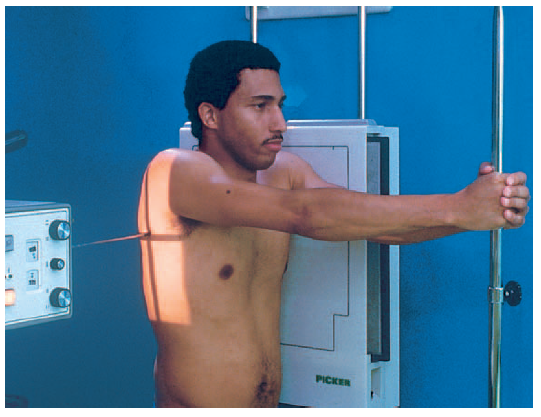
\includegraphics[width=0.7\linewidth]{imagenes/col26}
			\caption{}
			\label{fig:col26}
		\end{figure}
		
		
		\paragraph{Región de interés}
		La región abarca desde C7 hasta L1--L2, incluyendo los pasajes cervicotorácico y toracolumbar. Los brazos del paciente se dirigen hacia adelante (no hacia arriba), con el objetivo de desplazar el húmero fuera del pasaje cervicotorácico, desplegar los agujeros intervertebrales y elevar las costillas. Elevar los brazos provocaría superposición del húmero sobre T1--T3. Si la columna no es paralela al RI, se colocan soportes bajo la zona lumbar y se alinean hombros y cadera. Cuando el paciente está en decúbito, la espalda debe quedar orientada hacia el operador.
		
		\paragraph{Rayo Central}
		Perpendicular al plano del receptor. Punto de entrada: \textbf{T6/T7 (borde inferior de la escápula)}, cuatro traveses de dedos por dentro del reborde cutáneo posterior.
		
		\paragraph{Receptor de imagen}
		Centrado en T6/T7. Borde superior del RI ubicado 4--5 cm por encima de los hombros, de manera que el campo abarque desde C7 hasta L1--L2.
		
		\paragraph{Respiración}
		Técnica especial de respiración: se le indica al paciente que respire normalmente (inspire y espire) durante todo el tiempo de exposición. El tiempo de disparo se extiende a 1400--1600 ms para abarcar al menos un ciclo respiratorio completo. El movimiento de los arcos costales genera borrosidad cinética sobre éstos, eliminando su superposición sobre los cuerpos vertebrales y permitiendo visualizar la columna con mayor nitidez. Esto se obtiene separando el mA de los segundos en el equipo y ajustando el tiempo de exposición según el foco utilizado.
		
		\subsubsection*{4. Anatomía Visible}
		
		Se visualizan las 12 vértebras torácicas de perfil, con cuerpos vertebrales superpuestos entre sí (imagen de cuerpo único) y espacios discales abiertos. La región abarca desde C7 hasta L1--L2. Los arcos costales aparecen borrados por borrosidad cinética (técnica respiratoria). Las vértebras T1 a T3 pueden no visualizarse correctamente por superposición de los hombros. La línea posterolateral de los bordes posteriores debe presentarse como una línea única continua, lo que confirma la correcta superposición de los cuerpos vertebrales.
		
		\subsubsection*{5. Criterios de Evaluación}
		
		\textbf{Posicionamiento correcto:} Cuerpos vertebrales superpuestos de perfil formando una imagen única; espacios discales abiertos en toda la extensión; las 12 vértebras torácicas centradas en el RI; bordes posteriores formando una línea posterolateral única y continua.
		
		\textbf{Ausencia de rotación:} Superposición simétrica de las costillas homólogas entre sí; ausencia de doble línea en los bordes posteriores de los cuerpos vertebrales. La presencia de doble línea o falta de superposición costal indica rotación del paciente.
		
		\textbf{Penetración y contraste:} Amplia latitud de exposición. Vértebras claramente visibles a través de las sombras costales y pulmonares. Los arcos costales presentan borrosidad cinética uniforme. Colimación estrecha para reducir la radiación dispersa.
		
		\subsubsection*{6. Puntos Críticos}
		
		\textbf{Rotación del paciente:} Genera doble línea en los bordes posteriores de los cuerpos vertebrales y pérdida de superposición costal. Corrección: alinear hombros y caderas en el mismo plano, colocar soportes bajo la zona lumbar para que el eje longitudinal de la columna quede paralelo al RI, flexionar rodillas para estabilizar la posición.
		
		\textbf{No visualización de T1--T3:} Producida por superposición de los hombros y subexposición relativa en esa zona. El número de vértebras visibles depende del tamaño y la forma del paciente. No es un error corregible en todos los casos; se documenta como limitación de la proyección.
		
		\textbf{Adaptaciones:} En pacientes con dolor agudo o pediátricos se evalúa no utilizar la técnica respiratoria, dado que implica mayor tiempo de exposición y mayor dosis. En decúbito lateral, si la columna no es paralela al RI, se colocan soportes bajo la región lumbar para corregir la angulación.
		
		\textbf{Trucos:} La posición en decúbito lateral izquierdo se prefiere para acercar el corazón al RI y reducir la magnificación cardíaca. Los brazos deben dirigirse hacia adelante y no hacia arriba: esta diferencia es clave para evitar superposición del húmero en el pasaje cervicotorácico y para elevar las costillas. Al separar mA de segundos en el equipo, cambiar el foco recalcula automáticamente los milisegundos necesarios. La técnica respiratoria equivale a mayor dosis: la indicación depende de la calidad diagnóstica requerida y del estado del paciente.
		
		
		\onecolumn
		\clearpage
		
		\begin{figure}
			\centering
			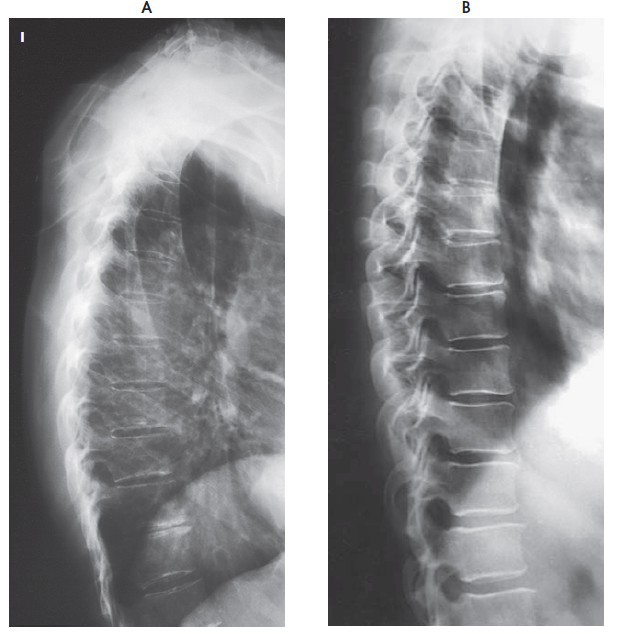
\includegraphics[width=0.7\linewidth]{imagenes/col28}
			\caption{Proyección lateral torácica.\textbf{ A}. Respiración suspendida con una exposición de 0,5 s. \textbf{B}. Técnica en respiración con una exposición de 1,5 s. Obsérvese que las marcas pulmonares están difuminadas.
			}
			\label{fig:col28}
		\end{figure}
		
		
		\twocolumn
		\clearpage
		
		%----------------------------------------------------------
		%  Para agregar otro enfoque duplicá el bloque
		%  desde \subsection hasta \textbf{Trucos}
		%----------------------------------------------------------
		
		
	%%%%%%%%%%%%%%%%%%%%%%%%%%%%%%%%%%%%%%%%%%%%%%%%%%%%%%%%%%%
	%  SECCIÓN: Columna Lumbar
	%  Archivo: secciones/columna_lumbar.tex
	%  Sin preámbulo ni \begin{document} — lo maneja main.tex
		%%%%%%%%%%%%%%%%%%%%%%%%%%%%%%%%%%%%%%%%%%%%%%%%%%%%%%%%%%%
		
		\section{Columna Lumbar}
		
		\subsection{Frente AP-PA}
		
		\subsubsection*{1. Identificación}
		
		\textbf{Tipo:} Proyección básica. Forma par con la proyección lateral de columna lumbar.
		
		\textbf{Indicaciones clínicas principales:}
		\begin{itemize}
			\item Fracturas de columna lumbar
			\item Escoliosis y otras curvaturas vertebrales
			\item Procesos neoplásicos vertebrales
		\end{itemize}
		
		\subsubsection*{2. Técnica Base}
		
		\textbf{Receptor de imagen:} 35$\times$43 cm (exploración lumbosacra) o 30$\times$35 cm (solo lumbar). Orientación \textbf{longitudinal (vertical)}.
		
		\textbf{DFRI:} 100 cm.
		
		\textbf{Técnica:} Intermedia, ajustada según el biotipo del paciente. Se utiliza kVp alto para penetrar la zona densa de la columna, permitiendo visualizar los detalles óseos, los espacios interdiscales y las partes blandas. El mAs se ajusta según el biotipo del paciente.
		
		\textbf{Bucky:} Bucky mural o de mesa con grilla.
		
		\subsubsection*{3. Posicionamiento}
		
		\paragraph{Paciente}
		Decúbito supino (posición preferida para la rutina). Plano medio sagital perpendicular al receptor de imagen y centrado en la línea media de la rejilla. Se indica al paciente vaciarse la vejiga urinaria previamente. Se prefiere la posición de bipedestación en pacientes con dolor intenso para reducir las molestias de la exploración. Si el paciente está en decúbito, se lo tracciona desde las axilas (preguntar por prótesis antes de realizar tracción). El paciente debe estar descalzo para evitar diferencias en la altura por calzado.
		
		\begin{figure}[h]
			\centering
			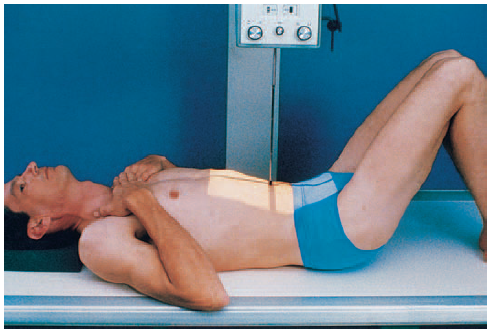
\includegraphics[width=0.7\linewidth]{imagenes/col29}
			\caption{}
			\label{fig:col29}
		\end{figure}
		
		
		\begin{figure}[h]
			\centering
			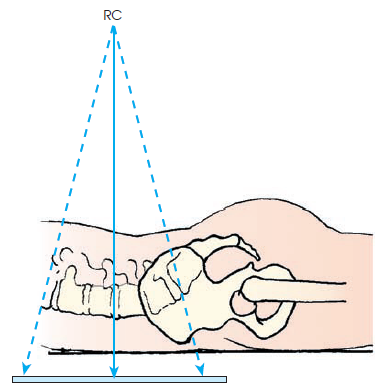
\includegraphics[width=0.7\linewidth]{imagenes/col30}
			\caption{}
			\label{fig:col30}
		\end{figure}
		
		
		\paragraph{Región de interés}
		Hombros y caderas ajustados en un mismo plano horizontal para evitar rotación. Codos flexionados con manos apoyadas sobre la parte superior del tórax, evitando que los antebrazos entren en el campo de exposición. Se reduce la lordosis lumbar mediante flexión suficiente de caderas y rodillas, colocando la espalda en contacto firme con la mesa. Se puede usar un soporte radiotransparente bajo la parte lateral inferior de la pelvis para reducir la rotación.
		
		\paragraph{Rayo Central}
		Perpendicular al plano del receptor. Para exploración \textbf{solo lumbar}: punto de entrada 4 cm por encima de las crestas ilíacas, incidiendo a nivel de L3. Para exploración \textbf{lumbosacra}: punto de entrada a la altura de las crestas ilíacas, incidiendo a nivel de L4.
		
		\paragraph{Receptor de imagen}
		Centrado en la región lumbar. Debe incluirse desde T12 hasta S1, abarcando una o dos vértebras torácicas inferiores, el sacro-cóccix y los huesos pélvicos. El colimador se ajusta hasta los márgenes laterales de los músculos psoas.
		
		\paragraph{Respiración}
		Suspendida al final de la espiración. La espiración máxima desplaza las vísceras abdominales y reduce la superposición de gas intestinal sobre las estructuras vertebrales, optimizando la nitidez de los cuerpos vertebrales y los espacios discales.
		
		\subsubsection*{4. Anatomía Visible}
		
		Se visualizan los cuerpos vertebrales lumbares (L1--L5), los espacios discales intervertebrales, los espacios interpedunculares, las láminas, y las apófisis espinosas y transversas. Las articulaciones sacroilíacas deben verse equidistantes de la columna vertebral. Las articulaciones intervertebrales deben estar abiertas. En estudios con RI de 35$\times$43 cm se incluyen además una o dos vértebras torácicas inferiores, el sacro, el cóccix y los huesos pélvicos. La sombra del músculo psoas debe ser visible como indicador de buena técnica de penetración.
		
		Para contar las vértebras lumbares se procede de abajo hacia arriba: partiendo de la vértebra ubicada por encima del sacro (L5), se numeran 5, 4, 3, 2 y 1, verificando que L1 sea la que porta costilla.
		
		\textbf{Ventaja de la proyección PA (prono-anterior):} La divergencia del haz de rayos, combinada con la lordosis lumbar, hace que los rayos divergentes pasen tangenciales a los espacios intervertebrales, manteniéndolos bien abiertos. Además reduce la dosis al paciente respecto de la posición AP. En caso de escoliosis detectada en el frente, se apoya el lado convexo contra el RI y el RC entra por el lado cóncavo, aprovechando la divergencia del haz para pasar tangencial a la curvatura.
		
		\subsubsection*{5. Criterios de Evaluación}
		
		\textbf{Posicionamiento correcto:} El área de imagen comprende desde las vértebras torácicas inferiores hasta el sacro. Las apófisis espinosas se visualizan centradas en los cuerpos vertebrales. Las articulaciones intervertebrales aparecen abiertas. La mitad de T12 debe ser visible; de no ser así, se repite la toma.
		
		\textbf{Ausencia de rotación:} Las articulaciones sacroilíacas se encuentran equidistantes de la columna vertebral. Las vértebras son simétricas en ambos lados del plano medio sagital. No debe haber asimetría en las apófisis transversas.
		
		\textbf{Penetración y contraste:} Todos los cuerpos vertebrales lumbares presentan penetración adecuada. La sombra del músculo psoas es visible bilateralmente. El colimado llega hasta los márgenes laterales del psoas, sin incluir partes blandas laterales innecesarias. Ausencia de artefactos producidos por elásticos de ropa interior.
		
		\subsubsection*{6. Puntos Críticos}
		
		\textbf{Rotación del paciente:} Produce asimetría de las articulaciones sacroilíacas y de los pedículos, dificultando la evaluación de los cuerpos vertebrales. Corregir alineando hombros y caderas en el mismo plano horizontal y verificando la perpendicularidad del plano medio sagital al RI.
		
		\textbf{Lordosis lumbar no corregida:} Los espacios intervertebrales aparecen cerrados, especialmente en los niveles L4--L5 y L5--S1, impidiendo su evaluación. Corregir mediante flexión de caderas y rodillas hasta que la espalda contacte firmemente con la mesa.
		
		\textbf{Adaptaciones:} En pacientes con dolor lumbar agudo, utilizar la posición en bipedestación para reducir las molestias. En pacientes con prótesis de cadera u hombro, evitar la tracción de axilas y utilizar otros métodos de estabilización. En pacientes obesos, aumentar el kVp para garantizar la penetración adecuada de la zona densa.
		
		\textbf{Trucos:} Al sospechar o confirmar escoliosis en la imagen, apoyar el lado convexo de la curvatura contra el RI y dirigir el RC desde el lado cóncavo para que los rayos divergentes pasen tangenciales a los espacios intervertebrales de la curva. Verificar siempre la presencia de T12 (con su costilla) para la correcta identificación y conteo vertebral de abajo hacia arriba.
		
		
		\onecolumn
		\clearpage
		
		\begin{figure}
			\centering
			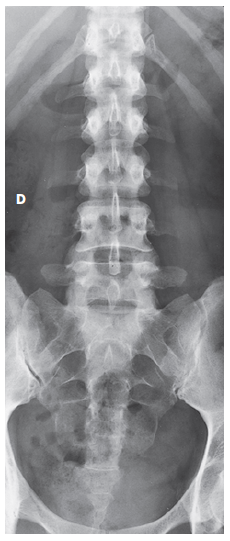
\includegraphics[width=0.5\linewidth]{imagenes/col31}
			\caption{}
			\label{fig:col31}
		\end{figure}
				
		\twocolumn
		\clearpage
		
		%----------------------------------------------------------
		%  Para agregar otro enfoque duplicá el bloque
		%  desde \subsection hasta \textbf{Trucos}
		%----------------------------------------------------------
		
	%%%%%%%%%%%%%%%%%%%%%%%%%%%%%%%%%%%%%%%%%%%%%%%%%%%%%%%%%%%
	%  SECCIÓN: Columna Lumbar
	%  Archivo: secciones/columna_lumbar.tex
	%  Sin preámbulo ni \begin{document} — lo maneja main.tex
		%%%%%%%%%%%%%%%%%%%%%%%%%%%%%%%%%%%%%%%%%%%%%%%%%%%%%%%%%%%
		
		\section{Columna Lumbar}
		
		\subsection{Lateral}
		
		\subsubsection*{1. Identificación}
		
		\textbf{Tipo:} Proyección básica. Forma par con la proyección AP de columna lumbar.
		
		\textbf{Indicaciones clínicas principales:}
		\begin{itemize}
			\item Fractura vertebral y espondilolistesis
			\item Osteoporosis de vértebras lumbares
			\item Procesos neoplásicos
			\item Evaluación de espacios discales y agujeros intervertebrales
		\end{itemize}
		
		\subsubsection*{2. Técnica Base}
		
		\textbf{Receptor de imagen:} 35$\times$43 cm para proyección lumbosacra; 30$\times$35 cm para columna lumbar exclusiva. Orientación \textbf{longitudinal}.
		
		\textbf{DFRI:} 100 cm. Distancia estándar para técnica homogeneizada.
		
		\textbf{Técnica:} Básica con kVp intermedio-alto para penetrar la zona densa de la columna y lograr visualización simultánea de detalles óseos, espacios interdiscales y partes blandas. Para evaluación de litiasis puede optarse por escala corta.
		
		\textbf{Bucky:} Sí. Uso obligatorio de Bucky con grilla por el alto grosor de la región.
		
		\subsubsection*{3. Posicionamiento}
		
		\paragraph{Paciente}
		Decúbito lateral (preferiblemente sobre el lado afectado o derecho para mayor comodidad operativa) o bipedestación lateral. Bata abierta por detrás para dejar la columna expuesta. Plano medio coronal perpendicular al receptor y centrado. El paciente se apoya sobre el lado de interés.
		
		\begin{figure}[h]
			\centering
			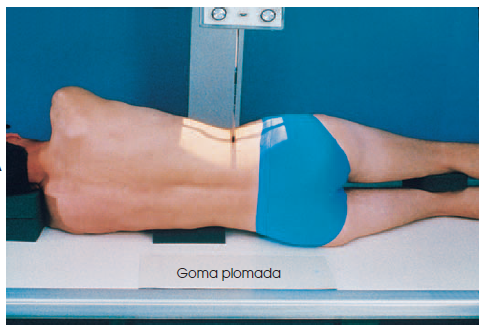
\includegraphics[width=0.7\linewidth]{imagenes/col32}
			\caption{}
			\label{fig:col32}
		\end{figure}
		
		
		\paragraph{Región de interés}
		Caderas y rodillas flexionadas cómodamente para reducir la lordosis lumbar. Las rodillas se superponen entre sí para prevenir la rotación pélvica. Se coloca almohadilla bajo la cabeza para mantener la columna horizontal. En pacientes con escoliosis, se apoya el lado convexo contra el receptor y el rayo central ingresa por el lado cóncavo, aprovechando el efecto de abanico para abrir los espacios intervertebrales. La región debe abarcar de T11--T12 hasta S1.
		
		\paragraph{Rayo Central}
		Perpendicular al receptor en condiciones estándar. Punto de entrada: \textbf{a la altura de la cresta ilíaca (L4--L5), 4 traveses de dedo por dentro del reborde cutáneo posterior}. La angulación se modifica según la morfología del paciente: angulación caudal de 5° en hombres y 8° en mujeres (según anchura de pelvis) cuando la columna no está horizontal; mayor angulación caudal ante pelvis más ancha. En columnas rectificadas no se requiere angulación. Para el pasaje L5--S1, se angula con mayor frecuencia; a mayor cadera, mayor angulación necesaria para abrir ese espacio.
		
		\paragraph{Receptor de imagen}
		Centrado a la altura de las crestas ilíacas (L4) para la proyección lumbosacra, o 4 cm por encima de las crestas ilíacas (L3) para la proyección lumbar exclusiva. Los bordes deben incluir desde T11--T12 hasta S1.
		
		\paragraph{Respiración}
		Suspendida al final de una espiración. La espiración completa reduce el diámetro anteroposterior del tronco, disminuye la superposición de estructuras y permite mayor nitidez en la imagen.
		
		\subsubsection*{4. Anatomía Visible}
		
		Se visualizan los cuerpos vertebrales lumbares de perfil, con sus bordes posteriores superpuestos entre sí como criterio de ausencia de rotación. Los espacios intervertebrales deben aparecer abiertos y bien definidos. Los agujeros intervertebrales se muestran abiertos, lo que permite evaluar su morfología. Las apófisis espinosas se proyectan de perfil. Las crestas ilíacas deben aparecer superpuestas cuando el haz no está angulado. Las escotaduras ciáticas mayores también deben superponerse.
		
		\subsubsection*{5. Criterios de Evaluación}
		
		\textbf{Posicionamiento correcto:} Espacios discales intervertebrales y agujeros intervertebrales abiertos. Apófisis espinosas proyectadas de perfil. Región abarcada desde T11--T12 hasta S1.
		
		\textbf{Ausencia de rotación:} Bordes posteriores de cada cuerpo vertebral superpuestos entre sí. Crestas ilíacas superpuestas (en proyección sin angulación). Escotaduras ciáticas mayores superpuestas. Si los cuerpos vertebrales presentan su base superior e inferior desplazadas entre sí (una adelante y otra atrás), indica que el paciente no está completamente de perfil.
		
		\textbf{Penetración y contraste:} Visualización clara y simultánea de estructuras óseas, espacios interdiscales y partes blandas. La técnica de kVp intermedio-alto debe permitir penetrar la zona densa de la columna sin sobreexponer las partes blandas periféricas.
		
		\subsubsection*{6. Puntos Críticos}
		
		\textbf{Rotación corporal:} Produce desalineación de los bordes posteriores vertebrales y de las crestas ilíacas, generando superposición asimétrica que impide la evaluación. Corrección: superponer rodillas, colocar saco de arena entre ellas y verificar que el plano medio coronal quede perpendicular al receptor.
		
		\textbf{Columna no horizontal:} Genera apertura desigual de los espacios intervertebrales. Corrección: colocar apoyo radiotransparente bajo el tórax inferior (método de elección) o aplicar angulación caudal del rayo central (5° en hombres, 8° en mujeres como promedio, ajustando según anchura de pelvis).
		
		\textbf{Adaptaciones:} En pacientes delgados, colocar almohadilla en la cadera declive para horizontalizar la columna. En pacientes con escoliosis, apoyar el lado convexo contra el receptor y dirigir el RC por el lado cóncavo. Para el segmento L5--S1, aumentar la angulación caudal según la anchura de la pelvis del paciente.
		
		\textbf{Trucos:} Colocar el brazo inferior perpendicular al cuerpo para estabilizar al paciente. El saco de arena entre rodillas superpuestas previene la rotación pélvica eficazmente. La rotación residual se detecta observando los cuerpos vertebrales: si la base superior e inferior de un mismo cuerpo no se superponen, el paciente está rotado. En escoliosis, el efecto de abanico al apoyar la convexidad permite abrir los espacios intervertebrales del lado cóncavo.
		
		\onecolumn
		\clearpage
		
		\begin{figure}
			\centering
			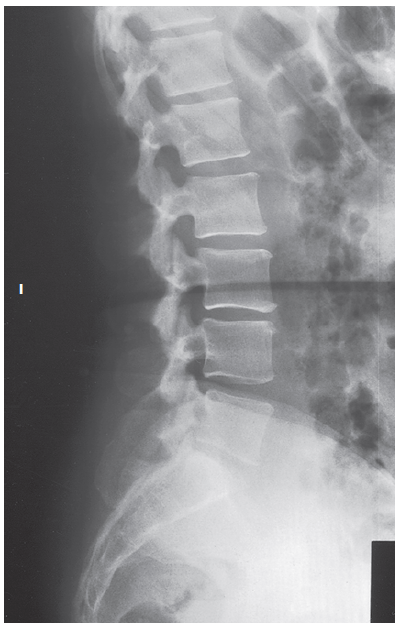
\includegraphics[width=0.7\linewidth]{imagenes/col33}
			\caption{}
			\label{fig:col33}
		\end{figure}
		
		\twocolumn
		\clearpage
		
		%----------------------------------------------------------
		%  Para agregar otro enfoque duplicá el bloque
		%  desde \subsection hasta \textbf{Trucos}
		%----------------------------------------------------------
		
	%%%%%%%%%%%%%%%%%%%%%%%%%%%%%%%%%%%%%%%%%%%%%%%%%%%%%%%%%%%
	%  SECCIÓN: Columna Lumbar
	%  Archivo: secciones/columna_lumbar.tex
	%  Sin preámbulo ni \begin{document} — lo maneja main.tex
		%%%%%%%%%%%%%%%%%%%%%%%%%%%%%%%%%%%%%%%%%%%%%%%%%%%%%%%%%%%
		
		\section{Columna Lumbar}
		
		\subsection{Charnela Lumbosacra (L5-S1) - Proyección Lateral}
		
		\subsubsection*{1. Identificación}
		
		\textbf{Tipo:} Complementario.
		
		\textbf{Indicaciones clínicas principales:}
		\begin{itemize}
			\item Espondilolistesis: deslizamiento anterior o posterior de una vértebra respecto a la adyacente, frecuente en el segmento L4-L5 hasta S1.
			\item Espondilosis: degeneración discovertebal que debilita el hueso, afecta principalmente L5-S1.
			\item Discopatías y estenosis del canal en la charnela lumbosacra.
		\end{itemize}
		
		\subsubsection*{2. Técnica Base}
		
		\textbf{Receptor de imagen:} 18$\times$24 cm. Orientación \textbf{longitudinal} (vertical), adaptada al eje mayor de la región lumbosacra.
		
		\textbf{DFRI:} 100 cm. Distancia estándar para columna lumbar.
		
		\textbf{Técnica:} Intermedia en pacientes estándar (kVp alto para penetrar la zona densa de la columna y visualizar detalles óseos, espacios interdiscales y partes blandas). Básica en pacientes con mayor grosor corporal. Debe compensarse la colimación reducida aplicando un incremento del 50--75\% en los factores, calculado mediante regla de tres.
		
		\textbf{Bucky:} Sí, con rejilla antidifusora (Bucky de mesa).
		
		\subsubsection*{3. Posicionamiento}
		
		\paragraph{Paciente}
		Decúbito lateral sobre la mesa radiológica. En caso de inestabilidad o sospecha de trauma, puede realizarse de pie. El plano medio sagital (PMS) de la cabeza debe ubicarse en el mismo plano que el eje longitudinal de la columna, utilizando una almohada de apoyo.
		
		\begin{figure}[h]
			\centering
			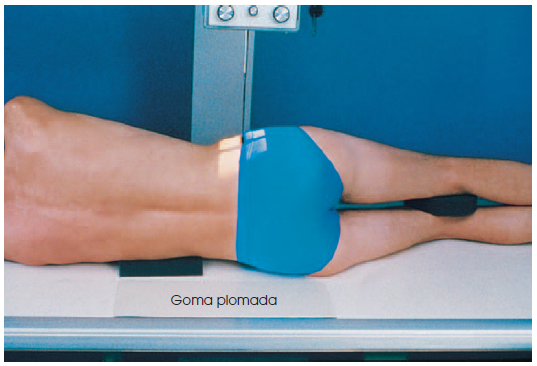
\includegraphics[width=0.7\linewidth]{imagenes/col34}
			\caption{}
			\label{fig:col34}
		\end{figure}
	
		\paragraph{Región de interés}
		El plano medio coronal (PMC) del cuerpo debe quedar perpendicular al receptor de imagen. Se superponen las rodillas con un apoyo entre ellas para evitar la rotación pélvica. Si es posible, las caderas se extienden completamente. Se puede colocar un soporte radiotransparente bajo la parte inferior del tórax para que el eje longitudinal de la columna quede en posición horizontal verdadera, lo que es el método de elección. El brazo inferior se flexiona en el codo y se posiciona perpendicular al cuerpo.
		
		\paragraph{Rayo Central}
		Perpendicular al receptor cuando la columna está correctamente horizontalizada. Punto de entrada: \textbf{5 cm posterior a la EIAS elevada y 4 cm inferior a la cresta ilíaca}. Para localizar el PMC se apoya una mano sobre el reborde cutáneo posterior del paciente y se avanzan 4 dedos hacia adelante; para la altura, se palpa la cresta ilíaca y se descienden 2 dedos.
		
			
		
		\begin{figure}[h]
			\centering
			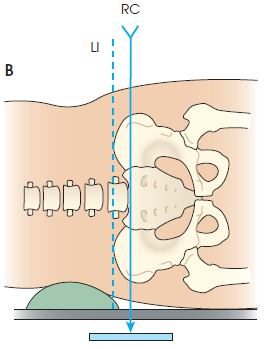
\includegraphics[width=0.7\linewidth]{imagenes/col35}
			\caption{}
			\label{fig:col35}
		\end{figure}
		
		
		
		Cuando la columna no puede horizontalizarse, se angula el RC en sentido \textbf{caudal 5° en hombres} y \textbf{8° en mujeres}, ingresando por la EIAS, para mejorar la apertura del espacio intervertebral L5-S1.
		
		\textit{Técnica alternativa de Francis:} localizar ambas crestas ilíacas, trazar una línea imaginaria entre ellas (plano interilíaco) y dirigir el RC paralelo a dicha línea.
		
		\begin{figure}[h]
			\centering
			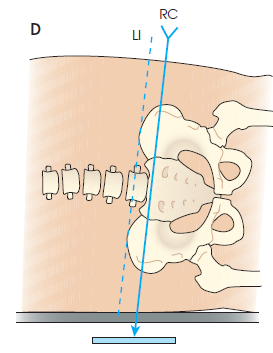
\includegraphics[width=0.7\linewidth]{imagenes/col37}
			\caption{}
			\label{fig:col37}
		\end{figure}
		
		
		\textit{Referencia angular adicional:} el espacio L5-S1 presenta una orientación oblicua de 10--15° condicionada por la lordosis lumbar y la inclinación sacra (35--50° respecto a la horizontal). Esto implica que, para obtener incidencia perpendicular al espacio intervertebral sin horizontalización, serían necesarios 30--35° en sentido craneal o 10--15° en sentido caudal según la variante anatómica individual.
		
		\paragraph{Receptor de imagen}
		Centrado en la articulación L5-S1. Colimación estrecha sobre la charnela lumbosacra. El área de exposición debe incluir los cuerpos vertebrales de L5 y S1 completos, y la parte superior del sacro.
		
		\paragraph{Respiración}
		Suspendida durante la exposición para eliminar microdesplazamientos de las estructuras óseas adyacentes.
		
		\subsubsection*{4. Anatomía Visible}
		
		Se visualiza la unión lumbosacra (L5-S1) con el espacio intervertebral completamente abierto, la vértebra L5 íntegra y la parte superior del sacro (S1). Las apófisis espinosas se proyectan de perfil. Las crestas ilíacas deben aparecer casi superpuestas entre sí cuando el RC no está angulado. La charnela lumbosacra ocupa el centro del área de exposición.
		
		\subsubsection*{5. Criterios de Evaluación}
		
		\textbf{Posicionamiento correcto:} articulación intervertebral lumbosacra L5-S1 completamente abierta; toda la vértebra L5 y la parte superior del sacro incluidas dentro del área colimada; charnela lumbosacra centrada en el área de exposición.
		
		\textbf{Ausencia de rotación:} crestas ilíacas casi superpuestas entre sí (cuando el RC no está angulado); apófisis espinosas proyectadas de perfil sin oblicuidad.
		
		\textbf{Penetración y contraste:} adecuada visualización de las estructuras óseas densas de la charnela; contraste suficiente para diferenciar los espacios discales y las partes blandas perivertebral.
		
		\subsubsection*{6. Puntos Críticos}
		
		\textbf{Espacio articular L5-S1 cerrado:} consecuencia de no aplicar la angulación caudal cuando la columna no está en posición horizontal verdadera. Corregir horizontalizando la columna con soporte radiotransparente bajo el tórax inferior, o angulando el RC 5° (hombres) u 8° (mujeres) en sentido caudal.
		
		\textbf{Rotación pélvica:} impide la superposición de las crestas ilíacas y genera proyección oblicua de las apófisis espinosas. Corregir verificando que las rodillas estén exactamente superpuestas con apoyo intermedio antes de exponer.
		
		\textbf{Adaptaciones:} en pacientes con trauma o inestabilidad, mantener la posición lateral sin movilizaciones excesivas; puede realizarse de pie si es necesario. Cuando no se pueda horizontalizar la columna, aplicar la técnica alternativa de Francis. En pacientes con cintura grande puede requerirse angulación cefálica del RC.
		
		\textbf{Trucos:} la EIAS elevada es fácilmente palpable con el paciente en decúbito lateral y constituye el punto de referencia estandarizado para centrar en L5-S1. El soporte radiotransparente bajo el tórax es el método de elección para horizontalizar la columna. Compensar la colimación estrecha incrementando los factores técnicos un 50--75\% (calcular mediante regla de tres). Verificar superposición de rodillas antes de la exposición.
		
		\onecolumn
		\clearpage
		
		\begin{figure}
			\centering
			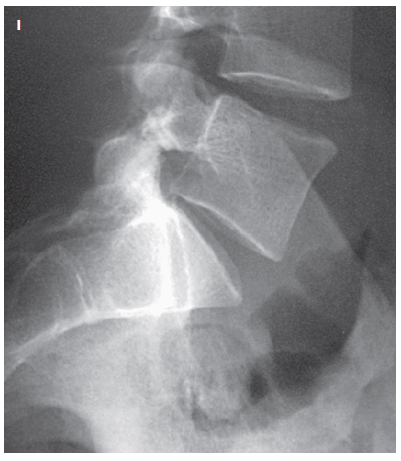
\includegraphics[width=0.7\linewidth]{imagenes/col36}
			\caption{}
			\label{fig:col36}
		\end{figure}
		
		
		\twocolumn
		\clearpage
		
		%----------------------------------------------------------
		%  Para agregar otro enfoque duplicá el bloque
		%  desde \subsection hasta \textbf{Trucos}
		%----------------------------------------------------------
		
	%%%%%%%%%%%%%%%%%%%%%%%%%%%%%%%%%%%%%%%%%%%%%%%%%%%%%%%%%%%
	%  SECCIÓN: Columna Lumbar
	%  Archivo: secciones/columna_lumbar_oblicua.tex
	%  Sin preámbulo ni \begin{document} — lo maneja main.tex
		%%%%%%%%%%%%%%%%%%%%%%%%%%%%%%%%%%%%%%%%%%%%%%%%%%%%%%%%%%%
		
		\section{Columna Lumbar}
		
		\subsection{AP Oblicua (OPD / OPI)}
		
		\subsubsection*{1. Identificación}
		
		\textbf{Tipo:} Proyección complementaria. Se realizan ambas oblicuas en conjunto de forma comparativa bilateral.
		
		\textbf{Indicaciones clínicas principales:}
		\begin{itemize}
			\item Evaluación de articulaciones interapofisarias y pars interarticularis (espondilólisis, espondilolistesis)
			\item Dolor crónico de columna; también indicada como referencia anatómica previa a infiltración anestésica interapofisaria bajo arco en C
			\item Fracturas de pars interarticularis no visibles en proyecciones estándar
		\end{itemize}
		
		\subsubsection*{2. Técnica Base}
		
		\textbf{Receptor de imagen:} 35$\times$43 cm (o 30$\times$35 cm). Orientación \textbf{longitudinal}. Para estudio focalizado en la quinta articulación interapofisaria se reduce a 18$\times$24 cm.
		
		\textbf{DFRI:} 100 cm. Distancia estándar para columna lumbar que equilibra nitidez geométrica y magnificación.
		
		\textbf{Técnica:} Intermedia para paciente estándar; básica para paciente de mayor grosor corporal. Se emplea kVp alto para garantizar la penetración de la zona densa de la columna y obtener visibilidad adecuada de detalles óseos, espacios interdiscales y partes blandas. \textbf{kVp --- mAs:} \textit{[dato no suministrado]}.
		
		\textbf{Bucky:} Con Bucky de mesa.
		
		\subsubsection*{3. Posicionamiento}
		
		\paragraph{Paciente}
		Decúbito supino sobre la mesa radiográfica, o en bipedestación según capacidad del paciente. El decúbito es preferible: estabiliza la posición evitando que la pelvis rote independientemente del tronco, y en pacientes de gran tamaño corporal reduce el espesor efectivo, disminuyendo la radiación dispersa y mejorando la calidad de imagen.
		
		\begin{figure}[h]
			\centering
			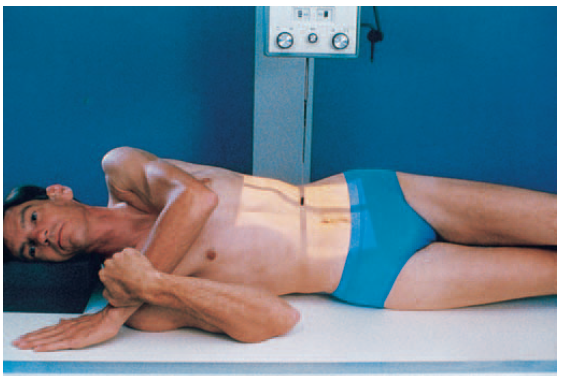
\includegraphics[width=0.7\linewidth]{imagenes/col38OPD}
			\caption{OPD}
			\label{fig:col38-opd}
		\end{figure}
		
		
		\paragraph{Región de interés}
		Partiendo del decúbito supino con el plano medio sagital perpendicular al receptor, se rota el cuerpo hacia el lado a estudiar aproximadamente \textbf{45°}. La \textbf{OPD} (rotación hacia la derecha) demuestra las articulaciones interapofisarias derechas; la \textbf{OPI} (rotación hacia la izquierda) demuestra las izquierdas. En ambos casos se visualizan las articulaciones del lado más próximo al receptor. Para las articulaciones de L5--S1 puede requerirse hasta \textbf{60°} de oblicuidad. Las articulaciones lumbares forman un ángulo de 30--60° con el plano sagital, por lo que la angulación varía según el nivel: menor angulación para articulaciones más superiores, mayor para las más inferiores. El eje longitudinal del paciente se mantiene paralelo al eje de la mesa. Se pueden colocar soportes bajo el hombro elevado, la cadera y la rodilla para evitar movimientos involuntarios.
		
		\paragraph{Rayo Central}
		Perpendicular al plano del receptor. Punto de entrada estándar: \textbf{5 cm medial a la EIAS elevada y 4 cm por encima de la cresta ilíaca} (nivel aproximado de L3). Para énfasis en la quinta articulación interapofisaria: \textbf{5 cm medial a la EIAS elevada y en el punto medio entre la cresta ilíaca y la EIAS}.
		
		\paragraph{Receptor de imagen}
		Centrado en la región lumbar media. El campo debe abarcar desde las vértebras torácicas inferiores hasta el sacro. La columna vertebral debe quedar paralela a la superficie del receptor para que los espacios intervertebrales T12--L1 y L1--L2 permanezcan abiertos.
		
		\paragraph{Respiración}
		Suspendida al final de una espiración completa. La espiración reduce el diámetro abdominal, disminuye la superposición de estructuras y minimiza el movimiento durante la exposición.
		
		\subsubsection*{4. Anatomía Visible}
		
		Se visualizan las articulaciones interapofisarias del lado más próximo al receptor, abiertas y uniformemente visibles a través de los cuerpos vertebrales. Se identifican las apófisis articulares superiores e inferiores y la pars interarticularis, estructura clave para detectar fracturas en espondilólisis y espondilolistesis.
		
		El criterio anatómico central es la imagen del \textbf{perro Scottie} (Proyección de La Chapelle): cuando el posicionamiento es correcto, cada vértebra lumbar adquiere la silueta de un perro escocés. Sus componentes son: el \textbf{ojo} corresponde al pedículo; la \textbf{oreja} a la apófisis articular superior (que articula con la apófisis articular inferior de la vértebra suprayacente, formando la ``pata''); el \textbf{hocico} a la apófisis transversa; el \textbf{cuello} a la pars interarticularis; y el \textbf{cuerpo} a la lámina. Una fractura de la pars interarticularis se evidencia como una línea radiolúcida en el cuello del perro, visible únicamente en proyección oblicua.
		
		Se aprecian además los cuerpos vertebrales, pedículos, espacios interdiscales y partes blandas paravertebrales.
		
		\begin{figure}[h]
			\centering
			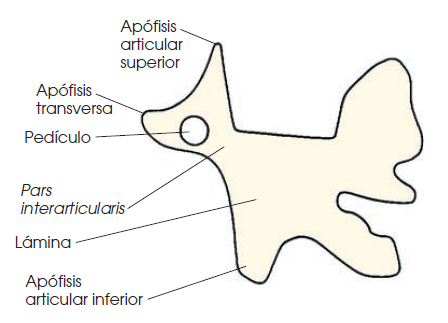
\includegraphics[width=0.7\linewidth]{imagenes/col39}
			\caption{}
			\label{fig:col39}
		\end{figure}
		
		
		\subsubsection*{5. Criterios de Evaluación}
		
		\textbf{Posicionamiento correcto:} La figura del perro Scottie se forma con nitidez en cada vértebra lumbar. Las articulaciones interapofisarias del lado estudiado se encuentran abiertas y visibles de forma uniforme. El pedículo se proyecta centrado sobre el cuerpo vertebral. Los espacios intervertebrales T12--L1 y L1--L2 están abiertos, confirmando que la columna es paralela al receptor.
		
		\textbf{Ausencia de rotación:} La oblicuidad es correcta cuando el pedículo se ubica sobre el cuerpo vertebral sin desplazamiento anterior ni posterior apreciable. La articulación interapofisaria aparece abierta y bien definida.
		
		\textbf{Penetración y contraste:} El kVp alto produce escala larga de grises que permite visualizar simultáneamente los detalles trabeculares óseos, los espacios interdiscales y las partes blandas adyacentes en una sola exposición.
		
		\subsubsection*{6. Puntos Críticos}
		
		\textbf{Rotación insuficiente:} El pedículo (ojo del perro) se proyecta anterior al cuerpo vertebral y la articulación interapofisaria no se abre. Corrección: aumentar la oblicuidad del paciente hacia el lado estudiado.
		
		\textbf{Rotación excesiva:} El pedículo se proyecta posterior al cuerpo vertebral. Corrección: reducir la oblicuidad del paciente.
		
		\textbf{Adaptaciones:} Para L5--S1 se incrementa la oblicuidad hasta 60° y, si el estudio es exclusivo de esa articulación, se utiliza RI de 18$\times$24 cm con RC en el punto medio entre la cresta ilíaca y la EIAS elevada. En pacientes de gran tamaño corporal, el decúbito es preferible al bipedestación por la estabilidad posicional y la reducción de la dispersión.
		
		\textbf{Trucos:} La identificación de la marca lateral sigue esta lógica: en una OPD los cuerpos vertebrales (estructura más anterior) se orientan hacia el lado derecho de la imagen y las apófisis espinosas hacia el lado opuesto; en la OPI, a la inversa. La comparación sistemática OPD--OPI es indispensable para diferenciar espondilólisis unilateral de espondilolistesis bilateral. En el contexto de infiltración interapofisaria, ambas oblicuas se solicitan en bloque y sirven como referencia anatómica previa al procedimiento bajo arco en C.
		
		
		\onecolumn
		\clearpage
		
		\begin{figure}
			\centering
			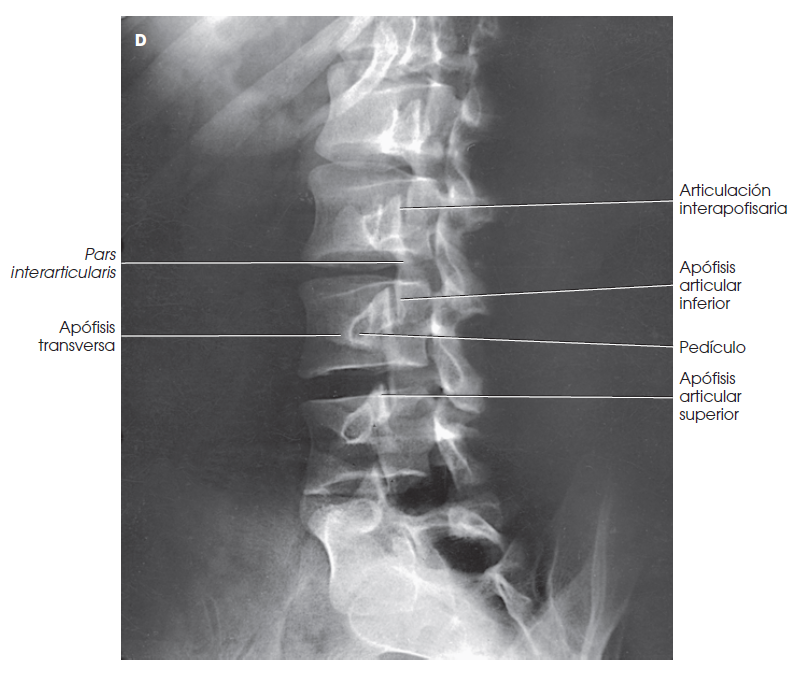
\includegraphics[width=0.7\linewidth]{imagenes/col40}
			\caption{}
			\label{fig:col40}
		\end{figure}
		
		
		\twocolumn
		\clearpage
		
		%----------------------------------------------------------
		%  Para agregar otro enfoque duplicá el bloque
		%  desde \subsection hasta \textbf{Trucos}
		%----------------------------------------------------------
		
	
	%%%%%%%%%%%%%%%%%%%%%%%%%%%%%%%%%%%%%%%%%%%%%%%%%%%%%%%%%%%
	%  SECCIÓN: Columna Lumbar
	%  Archivo: secciones/columna_lumbar_pa_oblicua.tex
	%  Sin preámbulo ni \begin{document} — lo maneja main.tex
		%%%%%%%%%%%%%%%%%%%%%%%%%%%%%%%%%%%%%%%%%%%%%%%%%%%%%%%%%%%
		
		\section{Columna Lumbar}
		
		\subsection{PA Oblicua (OAD / OAI)}
		
		\subsubsection*{1. Identificación}
		
		\textbf{Tipo:} Proyección complementaria. OAD y OAI son el mismo enfoque ejecutado hacia cada lado; se realizan en par para estudiar ambas columnas interapofisarias.
		
		\textbf{Indicaciones clínicas principales:}
		\begin{itemize}
			\item Defectos en la pars interarticularis (espondilólisis)
			\item Espondilolistesis
			\item Evaluación de las articulaciones interapofisarias del lado más alejado del RI
		\end{itemize}
		
		\subsubsection*{2. Técnica Base}
		
		\textbf{Receptor de imagen:} 35$\times$43 cm. Orientación \textbf{longitudinal} en paciente estándar. Para estudio exclusivo de la última articulación interapofisaria: 18$\times$24 cm.
		
		\textbf{DFRI:} 100 cm. Distancia estándar para radiografía de columna con Bucky de mesa o mural.
		
		\textbf{Técnica:} Intermedia en paciente estándar; básica (mayor carga) en paciente de mayor espesor.
		
		\textbf{Bucky:} Bucky con grilla. Uso obligatorio dado el espesor de la región lumbar.
		
		\subsubsection*{3. Posicionamiento}
		
		\paragraph{Paciente}
		Decúbito prono (posición preferida por mayor facilidad de inmovilización y menor porcentaje de repeticiones respecto a la oblicua AP). Alternativa: posición incorporada. Desde el decúbito prono, se rota al paciente hacia una posición de semiprono, apoyando el cuerpo sobre el antebrazo y la rodilla flexionados del lado que quedará elevado.
		
		\begin{figure}[h]
			\centering
			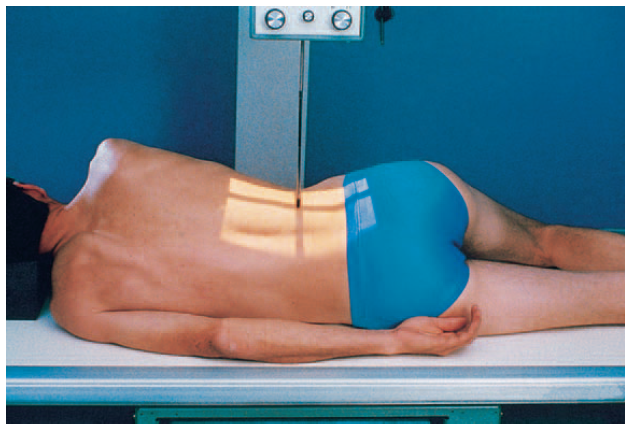
\includegraphics[width=0.7\linewidth]{imagenes/col41}
			\caption{OAI}
			\label{fig:col41}
		\end{figure}
		
		
		\paragraph{Región de interés}
		Rotación corporal oblicua de 45°; puede requerirse hasta 60° para demostrar correctamente las articulaciones interapofisarias de L5--S1 (charnela lumbosacra). La pierna del lado elevado se flexiona formando un ``4'' con la pierna contralateral extendida. Centrar L3 en la línea media de la rejilla. Para demostrar la charnela lumbosacra, centrar el RI sobre L5. La columna vertebral debe quedar paralela a la superficie de la mesa para mantener abiertos los espacios intervertebrales T12--L1 y L1--L2.
		
		\paragraph{Rayo Central}
		Perpendicular al plano del receptor. Punto de entrada: \textbf{L3, entre 2,5 y 3,8 cm por encima de la cresta ilíaca}, aproximadamente 5 cm lateral a las apófisis espinosas palpables. El RC entra siempre por el \textbf{lado elevado}.
		
		\paragraph{Receptor de imagen}
		Centrado en L3. La región a incluir abarca desde las vértebras torácicas inferiores (T12--L1) hasta el sacro. En la variante de 18$\times$24 cm, centrar sobre la última articulación interapofisaria de interés.
		
		\paragraph{Respiración}
		Suspendida al final de la espiración. La espiración completa reduce el espesor abdominal y la superposición de gas intestinal, mejorando el contraste de los elementos óseos posteriores.
		
		\subsubsection*{4. Anatomía Visible}
		
		Se demuestran las articulaciones interapofisarias del lado \textbf{más alejado del RI} (lado contrario al apoyo). En OAD el paciente apoya el lado derecho y se visualizan las articulaciones izquierdas; en OAI apoya el lado izquierdo y se visualizan las articulaciones derechas. Se incluyen las apófisis articulares superiores e inferiores, la pars interarticularis y la articulación T12--L1 en el RI de 35$\times$43 cm. La quinta articulación lumbosacra suele quedar bien visible. Los espacios intervertebrales T12--L1 y L1--L2 deben estar abiertos.
	
		Imagen del ``perro de Scottie'': figura radiológica característica de la oblicua lumbar cuyas partes corresponden a estructuras anatómicas específicas:
		\begin{itemize}
			\item \textbf{Ojo:} pedículo
			\item \textbf{Oreja:} apófisis articular superior
			\item \textbf{Hocico:} apófisis transversa
			\item \textbf{Cuello:} pars interarticularis
			\item \textbf{Cuerpo:} lámina
			\item \textbf{Patas delanteras:} apófisis articular inferior
		\end{itemize}
		
			
		\begin{figure}[h]
			\centering
			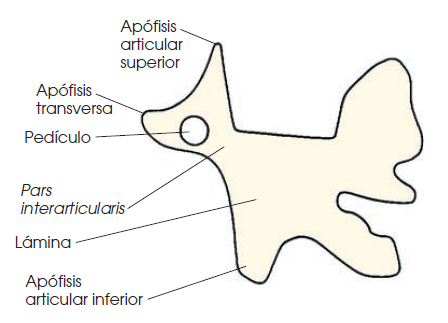
\includegraphics[width=0.7\linewidth]{imagenes/col39}
			\caption{}
			\label{fig:col98988}
		\end{figure}
		
		
		
		\textbf{Marca y orientación del cuerpo vertebral:}
		\begin{itemize}
			\item OAD: el cuerpo vertebral mira hacia la \textbf{izquierda} (lado contrario a la marca).
			\item OAI: el cuerpo vertebral mira hacia la \textbf{derecha} (mismo lado que la marca).
		\end{itemize}
		
		\subsubsection*{5. Criterios de Evaluación}
		
		\textbf{Posicionamiento correcto:} Articulaciones interapofisarias del lado más alejado del RI claramente abiertas y visibles. Columna vertebral paralela a la superficie de la mesa, con apertura de los espacios intervertebrales T12--L1 y L1--L2. Área cubierta desde las vértebras torácicas inferiores hasta el sacro.
		
		\textbf{Rotación insuficiente o excesiva:} Si la articulación interapofisaria no se visualiza bien y el pedículo aparece claramente anterior al cuerpo vertebral, la rotación es insuficiente (aumentar la oblicuidad). Si el pedículo aparece claramente posterior al cuerpo vertebral, la rotación es excesiva (reducir la oblicuidad).
		
		\textbf{Penetración y contraste:} Técnica adecuada cuando se distinguen con claridad las trabéculas óseas y los espacios articulares. Ajustar a técnica básica en pacientes de mayor espesor.
		
		\subsubsection*{6. Puntos Críticos}
		
		\textbf{Rotación insuficiente:} Las articulaciones interapofisarias no se abren y el pedículo se proyecta anterior al cuerpo vertebral. Corrección: aumentar la oblicuidad, hasta 60° si es necesario para L5--S1.
		
		\textbf{Aumento de la DORI:} La posición de semiprono incrementa la distancia objeto--receptor de imagen respecto a la oblicua AP, lo que puede reducir la resolución espacial. Es la principal desventaja de esta proyección frente a la AP oblicua.
		
		\textbf{Adaptaciones:} En paciente con limitaciones de movilidad o trauma, puede realizarse en posición incorporada. Verificar que se mantenga la oblicuidad de 45° con apoyo de cuñas radiolúcidas si es necesario.
		
		\textbf{Trucos:} Pedir al paciente que forme el número ``4'' con la pierna elevada estabiliza la rotación y facilita reproducir el ángulo. Regla práctica: en la PA oblicua lumbar siempre se visualizan las articulaciones del lado \textit{contrario} al apoyo, lo opuesto a las oblicuas torácicas.
		
		
		\onecolumn
		\clearpage
		
		\begin{figure}
			\centering
			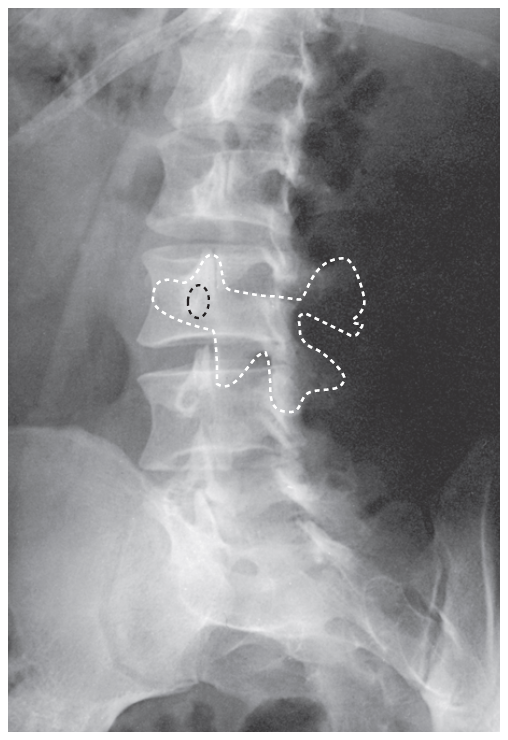
\includegraphics[width=0.7\linewidth]{imagenes/col42}
			\caption{OAI/OPD}
			\label{fig:col42}
		\end{figure}
		
		
		\twocolumn
		\clearpage
		
		%----------------------------------------------------------
		%  Para agregar otro enfoque duplicá el bloque
		%  desde \subsection hasta \textbf{Trucos}
		%----------------------------------------------------------
	
	
	%%%%%%%%%%%%%%%%%%%%%%%%%%%%%%%%%%%%%%%%%%%%%%%%%%%%%%%%%%%
	%  SECCIÓN: [Nombre de la Sección]
	%  Archivo: secciones/[nombre_archivo].tex
	%  Sin preámbulo ni \begin{document} — lo maneja main.tex
		%%%%%%%%%%%%%%%%%%%%%%%%%%%%%%%%%%%%%%%%%%%%%%%%%%%%%%%%%%%
		
		\section{Columna Lumbar}
		
		\subsection{Proyecciones Funcionales Lumbares - Hiperflexión / Hiperextensión}
		
		\subsubsection*{1. Identificación}
		
		\textbf{Tipo:} Complementaria. Forma par entre sí: se obtienen dos imágenes laterales, una en hiperflexión y otra en hiperextensión.
		
		\textbf{Indicaciones clínicas principales:}
		\begin{itemize}
			\item Valoración de la movilidad en sitio de artrodesis vertebral.
			\item Inestabilidad vertebral y subluxaciones.
			\item Localización de hernia discal (evidenciada por limitación del movimiento en el punto de la lesión).
		\end{itemize}
		
		\subsubsection*{2. Técnica Base}
		
		\textbf{Receptor de imagen:} 35$\times$43 cm. Orientación \textbf{longitudinal}, colocado en vertical. Borde inferior del RI 3--5 cm por debajo de la cresta ilíaca.
		
		\textbf{DFRI:} 100 cm. Distancia estándar para la región en posición de perfil.
		
		\textbf{Técnica:} Contrastada (alto contraste) con kV moderado. El alto contraste permite definir con precisión los bordes óseos para detectar posibles desplazamientos vertebrales; el kV moderado garantiza la penetración adecuada de la región en posición lateral durante los movimientos de flexo-extensión.
		
		\textbf{Bucky:} Sí, con rejilla.
		
		\subsubsection*{3. Posicionamiento}
		
		\paragraph{Paciente}
		De pie, descalzo y en carga con peso distribuido equitativamente entre ambos pies. Al ser una proyección funcional debe realizarse de pie. Como alternativa puede realizarse en decúbito lateral. La pelvis permanece inmóvil durante toda la exploración.
		
		\begin{figure}[h]
			\centering
			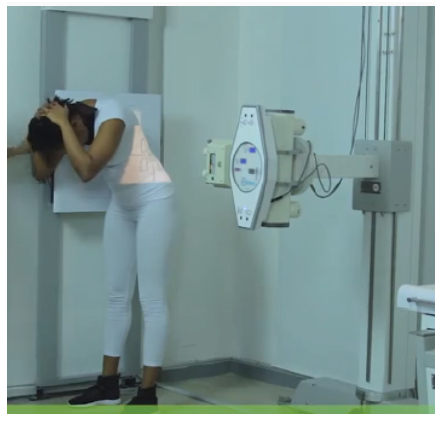
\includegraphics[width=0.7\linewidth]{imagenes/col43}
			\caption{Flexión}
			\label{fig:col43}
		\end{figure}
		
		\begin{figure}
			\centering
			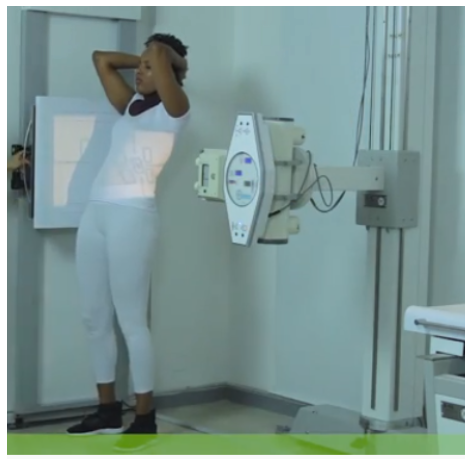
\includegraphics[width=0.7\linewidth]{imagenes/col44}
			\caption{Extensión}
			\label{fig:col44}
		\end{figure}
		
		
		\paragraph{Región de interés}
		Plano medio sagital paralelo al receptor. Se incluye desde T12 hasta la parte superior del cóccix, con bordes posterior y anterior sin cortar las apófisis espinosas.
		
		\paragraph{Rayo Central}
		Perpendicular al plano del receptor. Punto de entrada: \textbf{4 cm por encima de las crestas ilíacas}.
		
		\paragraph{Receptor de imagen}
		Vertical (longitudinal). Centrado a nivel del RC. Borde inferior 3--5 cm por debajo de la cresta ilíaca. Colimación a los 4 lados del área de interés.
		
		\paragraph{Respiración}
		Suspendida en espiración. Favorece la relajación muscular y facilita los movimientos de flexión y extensión. Se realizan dos exposiciones separadas, una por posición.
		
		\subsubsection*{4. Anatomía Visible}
		
		Cuerpos vertebrales de T12, L1--L5, sacro y parte superior del cóccix. Discos intervertebrales, espacios discales y apófisis espinosas de perfil. Articulaciones interapofisiarias.
		
		En \textbf{hiperflexión}: mayor separación entre apófisis espinosas y menor espacio entre cuerpos vertebrales. En \textbf{hiperextensión}: menor espacio entre apófisis espinosas y mayor espacio entre cuerpos vertebrales.
		
		\subsubsection*{5. Criterios de Evaluación}
		
		\textbf{Posicionamiento correcto:} En hiperflexión, el paciente se inclina hacia adelante sin doblar rodillas ni desplazar la pelvis hacia atrás; en decúbito lateral, muslos elevados al máximo. En hiperextensión, el paciente se inclina hacia atrás como intentando mirar el techo, con pies firmes en el suelo. Los marcadores identificadores (hiperflexión / hiperextensión) deben estar correctamente utilizados en cada proyección.
		
		\textbf{Ausencia de rotación:} Márgenes posteriores de los cuerpos vertebrales superpuestos, sin rotación de la columna vertebral.
		
		\textbf{Penetración y contraste:} Bordes óseos de los cuerpos vertebrales y apófisis espinosas bien definidos con alto contraste. Espacios discales y apófisis espinosas claramente diferenciables en ambas posiciones, permitiendo valorar la movilidad en el sitio de artrodesis o restricción por lesión.
		
		\subsubsection*{6. Puntos Críticos}
		
		\textbf{Rotación vertebral:} Produce superposición asimétrica de los márgenes vertebrales, impidiendo la correcta valoración de la movilidad. Corregir alineando el plano medio sagital paralelo al RI y verificando que pelvis y hombros queden en el mismo plano.
		
		\textbf{Insuficiente amplitud de movimiento:} Imágenes con escasa diferencia entre ambas posiciones no permiten valorar la movilidad articular. Guiar al paciente verbalmente con referencias concretas (``doble la espalda como si quisiera tocarse los pies'' / ``inclínese hacia atrás como si quisiera mirar el techo'') sin forzar el movimiento.
		
		\textbf{Adaptaciones:} Si el paciente no tolera la bipedestación, puede realizarse en decúbito lateral; en esa posición se le solicita llevar los muslos hacia arriba (hiperflexión) o extender el torso y miembros hacia atrás (hiperextensión). Para la hiperextensión de pie puede utilizarse un soporte de suero, barras o barandas para que el paciente se afirme. Todos los movimientos deben ser cómodos y dentro del rango tolerable.
		
		\textbf{Trucos:} Preferir siempre la posición erguida por ser más fisiológica y reproducible. Utilizar marcadores identificadores en cada imagen para distinguir hiperflexión de hiperextensión. Valorar comparativamente los cambios en los espacios discales y en las apófisis espinosas entre ambas proyecciones para determinar si existe movilidad en el sitio de fusión o restricción por lesión.
		
		
		\clearpage
		\onecolumn
		
		\begin{figure}
			\centering
			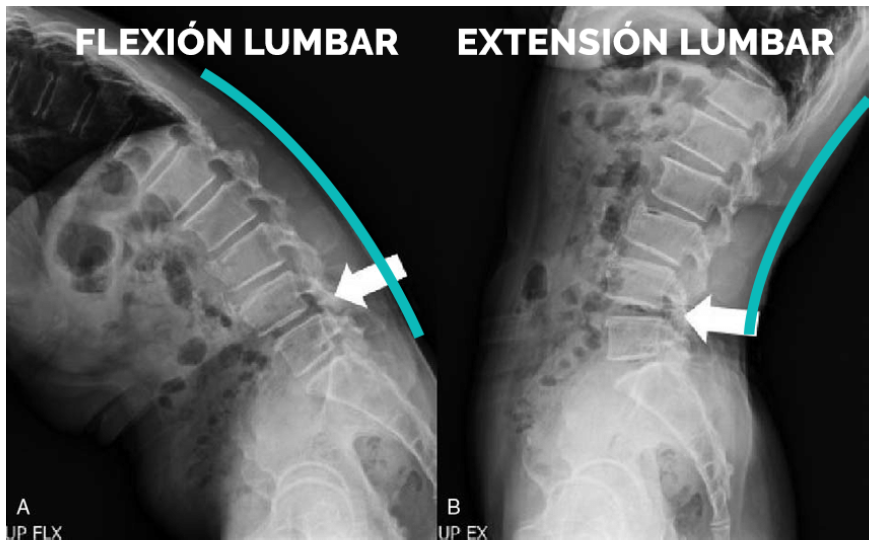
\includegraphics[width=0.7\linewidth]{imagenes/col45}
			\caption{}
			\label{fig:col45}
		\end{figure}
		
		
		\twocolumn
		\clearpage
		%----------------------------------------------------------
		%  Para agregar otro enfoque duplicá el bloque
		%  desde \subsection hasta \textbf{Trucos}
		%----------------------------------------------------------
		
		
	%%%%%%%%%%%%%%%%%%%%%%%%%%%%%%%%%%%%%%%%%%%%%%%%%%%%%%%%%%%
	%  SECCIÓN: Articulaciones Sacroilíacas
	%  Archivo: secciones/sacroiliacas_ap_pa_axial.tex
	%  Sin preámbulo ni \begin{document} — lo maneja main.tex
		%%%%%%%%%%%%%%%%%%%%%%%%%%%%%%%%%%%%%%%%%%%%%%%%%%%%%%%%%%%
		
		\section{Columna Sacra}
		
		\subsection{Proyección AP/PA Axial - Método de Ferguson}
		
		\subsubsection*{1. Identificación}
		
		\textbf{Tipo:} Proyección básica. Las variantes AP (supino) y PA (prono) son intercambiables según la condición del paciente; la PA en prono es la recomendada por Meese para las articulaciones sacroilíacas.
		
		\textbf{Indicaciones clínicas principales:}
		\begin{itemize}
			\item Fracturas de la articulación sacroilíaca
			\item Luxaciones y subluxaciones sacroilíacas
			\item Evaluación de la charnela lumbosacra (pasaje L5--S1)
		\end{itemize}
		
		\subsubsection*{2. Técnica Base}
		
		\textbf{Receptor de imagen:} 18$\times$24 cm o 24$\times$30 cm. Orientación \textbf{longitudinal} respecto al eje mayor de la región.
		
		\textbf{DFRI:} 100 cm.
		
		\textbf{Técnica:} Intermedia en paciente estándar --- Básica en paciente con gran espesor --- Homogenizada en niños o pacientes muy delgados.
		
		\textbf{Bucky:} Bucky de mesa con grilla.
		
		\subsubsection*{3. Posicionamiento}
		
		\paragraph{Paciente}
		\textbf{AP axial:} decúbito supino, plano medio sagital centrado en la rejilla.
		\textbf{PA axial:} decúbito prono (recomendado por Meese), plano medio sagital centrado en la rejilla. En prono, la oblicuidad natural de las articulaciones sacroilíacas las ubica más paralelas al receptor, y la divergencia del haz mejora su visualización sin necesidad de mayor angulación.
		
		\begin{figure}[h]
			\centering
			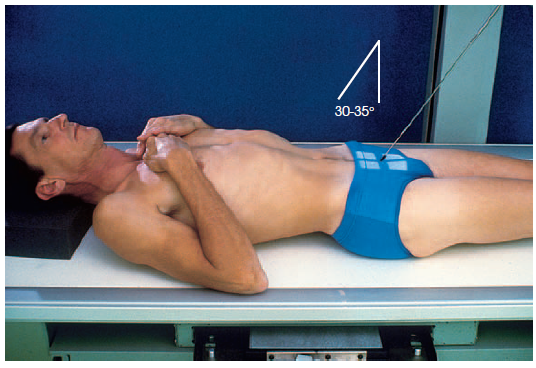
\includegraphics[width=0.7\linewidth]{imagenes/col46}
			\caption{}
			\label{fig:col46}
		\end{figure}
		
		\begin{figure}[h]
			\centering
			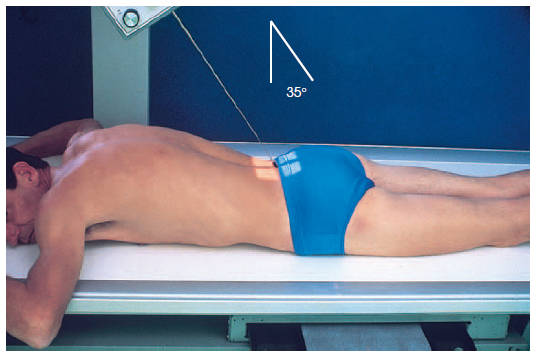
\includegraphics[width=0.7\linewidth]{imagenes/col48}
			\caption{}
			\label{fig:col48}
		\end{figure}
				
		
		\paragraph{Región de interés}
		En ambas variantes se extienden los miembros inferiores o se abducen los muslos, ajustándolos en posición vertical. Debe verificarse que la pelvis no esté rotada. La combinación de la oblicuidad articular y la divergencia del haz permite que el rayo incida de forma tangencial sobre las articulaciones sacroilíacas, mejorando su visualización. Se protegen las gónadas.
		
		\paragraph{Rayo Central}
		\textbf{AP axial:} angulado en dirección \textbf{cefálica}. En hombres: \textbf{30°}. En mujeres: \textbf{35°} (mayor lordosis y ángulo lumbosacro). Ferguson recomendó originalmente 45°; el rango de 30--35° es actualmente el estándar. Dirigido a través de la articulación lumbosacra. Punto de entrada: \textbf{4 cm por encima de la sínfisis del pubis, en el plano medio sagital}.
		
		\textbf{PA axial:} angulado en dirección \textbf{caudal}, con una angulación promedio de \textbf{35°}. Dirigido a través de la articulación lumbosacra hacia el punto medio del RI. Punto de entrada: \textbf{apófisis espinosa de L4}.
		
		La justificación de la angulación en ambos casos es la misma: las curvaturas de la columna impiden que el rayo pase tangencial al espacio articular sin angular; de ahí el calificativo \textit{axial}.
		
		\paragraph{Receptor de imagen}
		Centrado sobre el rayo central en ambas variantes. Los márgenes laterales deben incluir ambas articulaciones sacroilíacas sin cortarlas. La colimación se restringe al área de interés asegurando la inclusión de la charnela lumbosacra y el sacro completo.
		
		\paragraph{Respiración}
		Suspendida en el momento de la exposición. Evita el movimiento de estructuras abdominopélvicas que generarían borrosidad.
		
		\subsubsection*{4. Anatomía Visible}
		
		La imagen muestra la charnela lumbosacra (L5--S1) y el sacro. Se visualizan simétricamente ambas articulaciones sacroilíacas, libres de superposición. La angulación abre el espacio intervertebral entre L5 y S1, que de otra forma quedaría obliterado por las curvaturas de la columna. En la variante PA (Meese), el posicionamiento en prono acerca las articulaciones al plano paralelo al receptor, optimizando aún más su representación.
		
		\subsubsection*{5. Criterios de Evaluación}
		
		\textbf{Posicionamiento correcto:} espacio intervertebral L5--S1 abierto y visible; charnela lumbosacra y sacro incluidos en su totalidad.
		
		\textbf{Ausencia de rotación:} imagen simétrica de ambas articulaciones sacroilíacas, sin superposiciones que las oculten.
		
		\textbf{Penetración y contraste:} ambas articulaciones sacroilíacas adecuadamente penetradas, con densidad que permita distinguir el espacio articular.
		
		\subsubsection*{6. Puntos Críticos}
		
		\textbf{Angulación insuficiente:} el espacio intervertebral L5--S1 no se abre y las articulaciones sacroilíacas quedan superpuestas. Corregir ajustando los grados según el sexo del paciente y valorando visualmente el contorno de la zona lumbar baja para estimar la lordosis real.
		
		\textbf{Rotación pélvica:} asimetría de las articulaciones sacroilíacas en la imagen. Verificar que las EIAS equidisten del plano medio sagital antes de exponer.
		
		\textbf{Adaptaciones:} en pacientes con dolor o trauma agudo que no toleran el decúbito prono, utilizar la variante AP axial. Valorar la angulación según la lordosis real del paciente, aumentándola o reduciéndola respecto al promedio de 30--35°.
		
		\textbf{Trucos:} valorar el contorno de la parte inferior de la espalda para estimar una acentuación o disminución no habitual del ángulo lumbosacro y variar la angulación del RC en consecuencia. En la variante PA, el RC entra por la línea media aproximadamente 5 cm distal a la apófisis espinosa de L5, centrado a la altura de las EIAS.
		
		\clearpage
		\onecolumn
		
		\begin{figure}
			\centering
			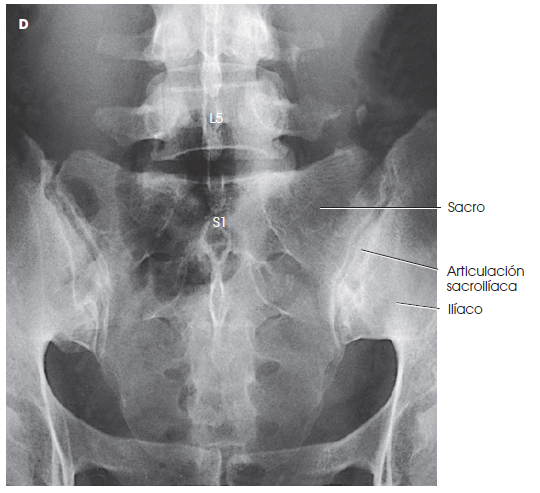
\includegraphics[width=0.7\linewidth]{imagenes/col47}
			\caption{AP}
			\label{fig:col47}
		\end{figure}
		
		\begin{figure}
			\centering
			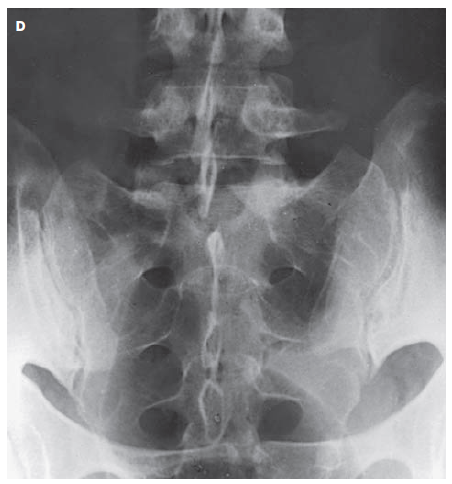
\includegraphics[width=0.7\linewidth]{imagenes/col49}
			\caption{PA}
			\label{fig:col49}
		\end{figure}
		
		
		\twocolumn
		\clearpage
		
		%----------------------------------------------------------
		%  Para agregar otro enfoque duplicá el bloque
		%  desde \subsection hasta \textbf{Trucos}
		%----------------------------------------------------------
	
	
	%%%%%%%%%%%%%%%%%%%%%%%%%%%%%%%%%%%%%%%%%%%%%%%%%%%%%%%%%%%
	%  SECCIÓN: Articulaciones Sacroilíacas
	%  Archivo: secciones/sacroiliacas_oblicua.tex
	%  Sin preámbulo ni \begin{document} — lo maneja main.tex
		%%%%%%%%%%%%%%%%%%%%%%%%%%%%%%%%%%%%%%%%%%%%%%%%%%%%%%%%%%%
		
		\section{Columna Sacra}
		
		\subsection{Proyección AP Oblicua (OPD / OPI) - Articulaciones Sacroilíacas}
		
		\subsubsection*{1. Identificación}
		
		\textbf{Tipo:} Proyección complementaria. Se realiza en ambas posiciones (OPD y OPI) para comparación bilateral.
		
		\textbf{Indicaciones clínicas principales:}
		\begin{itemize}
			\item Evaluación de luxación o subluxación de la articulación sacroilíaca.
			\item Procesos patológicos de la articulación sacroilíaca.
			\item Estudio comparativo bilateral de ambas articulaciones.
		\end{itemize}
		
		\subsubsection*{2. Técnica Base}
		
		\textbf{Receptor de imagen:} 24x30 cm. Orientación \textbf{longitudinal} (vertical). Se realizan ambas oblicuas.
		
		\textbf{DFRI:} 100 cm.
		
		\textbf{Técnica:} Básica para pacientes de gran espesor; intermedia para pacientes estándar; homogeneizada para pacientes muy delgados o pediátricos.
		
		\textbf{Bucky:} Bucky de mesa con grilla.
		
		\subsubsection*{3. Posicionamiento}
		
		\paragraph{Paciente}
		Decúbito supino. La cabeza se eleva sobre una almohada para mayor comodidad. Se eleva el lado en estudio aproximadamente 25--30°, apoyando el hombro, la parte inferior del tórax y la parte superior del muslo para mantener la oblicuidad.
		
		
		\begin{figure}[h]
			\centering
			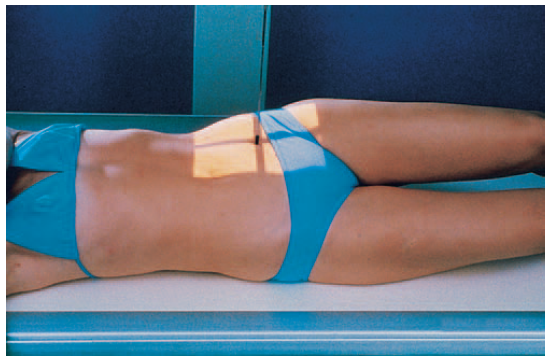
\includegraphics[width=0.7\linewidth]{imagenes/col50}
			\caption{AP OPD}
			\label{fig:col50}
		\end{figure}
		
		
		\paragraph{Región de interés}
		Se alinea el cuerpo de forma que un plano sagital que pase 2,5 cm medial a la EIAS del lado elevado quede centrado sobre la línea media de la rejilla. Se verifica la rotación en varios puntos a lo largo de la espalda. El lado en estudio es el más alejado del receptor de imagen: posición OPI para demostrar la articulación derecha; posición OPD para demostrar la articulación izquierda.
		
		\paragraph{Rayo Central}
		Perpendicular al plano del receptor. Punto de entrada: \textbf{2,5 cm medial a la EIAS del lado elevado}.
		
		\begin{figure}[h]
			\centering
			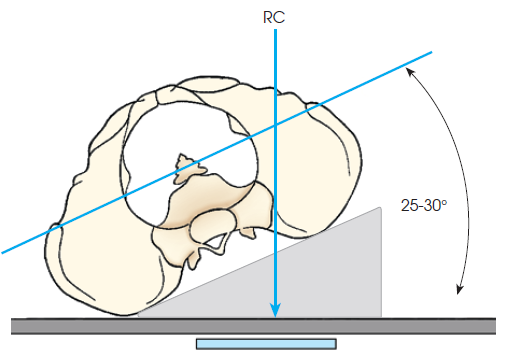
\includegraphics[width=0.7\linewidth]{imagenes/col51}
			\caption{}
			\label{fig:col51}
		\end{figure}
		
		
		\paragraph{Receptor de imagen}
		Centrado a la altura de la EIAS. Debe incluir la articulación sacroilíaca del lado en estudio con márgenes adecuados para su evaluación.
		
		\paragraph{Respiración}
		Suspendida durante la exposición.
		
		\subsubsection*{4. Anatomía Visible}
		
		Se visualiza la articulación sacroilíaca del lado más alejado del receptor (lado elevado). La oblicuidad proyecta la articulación de forma que solo se radiografía la porción más posterior de la misma; el rayo central no pasa tangencial a la parte anterior de la articulación. Esto es consecuencia de la oblicuidad propia de la articulación sacroilíaca, cuya orientación no es completamente coronal, sino que presenta un componente posterior y otro anterior.
		
		\subsubsection*{5. Criterios de Evaluación}
		
		\textbf{Posicionamiento correcto:} Espacio articular sacroilíaco abierto con mínima superposición del ilíaco y el sacro. La articulación debe quedar centrada en la radiografía.
		
		\textbf{Ausencia de rotación:} Oblicuidad de 25--30° correctamente mantenida, verificada por la apertura del espacio articular sacroilíaco sin exceso de superposición ósea.
		
		\textbf{Penetración y contraste:} Técnica adecuada al biotipo del paciente (básica, intermedia u homogeneizada), con visualización nítida de la interlínea articular sacroilíaca.
		
		\subsubsection*{6. Puntos Críticos}
		
		\textbf{Confusión de lado:} Recordar que el lado en estudio es el elevado (más alejado del RI). OPI demuestra la articulación derecha; OPD demuestra la izquierda.
		
		\textbf{Visualización parcial de la articulación:} Por la oblicuidad anatómica de la articulación sacroilíaca, solo se radiografía su porción posterior. No es posible obtener una imagen completa en una sola proyección oblicua, lo que limita la valoración. Este enfoque no es de uso común por esta razón.
		
		\textbf{Adaptaciones:} En pacientes con limitación para el decúbito supino, ajustar el apoyo con cuñas o almohadillas para mantener los 25--30° de oblicuidad.
		
		\textbf{Trucos:} Siempre explorar ambos lados para comparación bilateral. La radioprotección gonadal es de aplicación obligatoria en varones mediante colimación estrecha centrada en la articulación; en mujeres es técnicamente difícil de aplicar sin comprometer la región de interés.
		
		
		\onecolumn
		\clearpage
		
		\begin{figure}
			\centering
			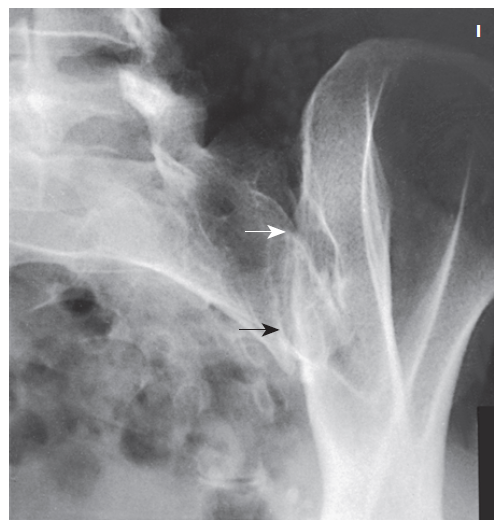
\includegraphics[width=0.7\linewidth]{imagenes/col52}
			\caption{}
			\label{fig:col52}
		\end{figure}
		
		
		\twocolumn
		\clearpage
		%----------------------------------------------------------
		%  Para agregar otro enfoque duplicá el bloque
		%  desde \subsection hasta \textbf{Trucos}
		%----------------------------------------------------------
		
		
	%%%%%%%%%%%%%%%%%%%%%%%%%%%%%%%%%%%%%%%%%%%%%%%%%%%%%%%%%%%
	%  SECCIÓN: Articulaciones Sacroilíacas
	%  Archivo: secciones/sacroiliacas_oblicua.tex
	%  Sin preámbulo ni \begin{document} — lo maneja main.tex
		%%%%%%%%%%%%%%%%%%%%%%%%%%%%%%%%%%%%%%%%%%%%%%%%%%%%%%%%%%%
		
		\section{Columna Sacra}
		
		\subsection{Proyección AP Oblicua (OPD / OPI) - Articulaciones Sacroilíacas}
		
		\subsubsection*{1. Identificación}
		
		\textbf{Tipo:} Proyección complementaria. Se realiza en ambas posiciones (OPD y OPI) para comparación bilateral.
		
		\textbf{Indicaciones clínicas principales:}
		\begin{itemize}
			\item Evaluación de luxación o subluxación de la articulación sacroilíaca.
			\item Procesos patológicos de la articulación sacroilíaca.
			\item Estudio comparativo bilateral de ambas articulaciones.
		\end{itemize}
		
		\subsubsection*{2. Técnica Base}
		
		\textbf{Receptor de imagen:} 24x30 cm. Orientación \textbf{longitudinal} (vertical). Se realizan ambas oblicuas.
		
		\textbf{DFRI:} 100 cm.
		
		\textbf{Técnica:} Básica para pacientes de gran espesor; intermedia para pacientes estándar; homogeneizada para pacientes muy delgados o pediátricos.
		
		\textbf{Bucky:} Bucky de mesa con grilla.
		
		\subsubsection*{3. Posicionamiento}
		
		\paragraph{Paciente}
		Decúbito supino. La cabeza se eleva sobre una almohada para mayor comodidad. Se eleva el lado en estudio aproximadamente 25--30°, apoyando el hombro, la parte inferior del tórax y la parte superior del muslo para mantener la oblicuidad.
		
		\begin{figure}[h]
			\centering
			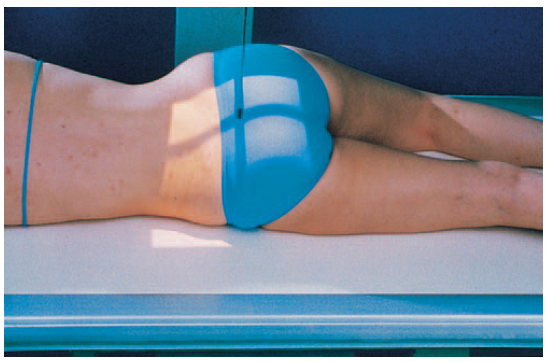
\includegraphics[width=0.7\linewidth]{imagenes/col53}
			\caption{}
			\label{fig:col53}
		\end{figure}
		
		
		\paragraph{Región de interés}
		Se alinea el cuerpo de forma que un plano sagital que pase 2,5 cm medial a la EIAS del lado elevado quede centrado sobre la línea media de la rejilla. Se verifica la rotación en varios puntos a lo largo de la espalda. El lado en estudio es el más alejado del receptor de imagen: posición OPI para demostrar la articulación derecha; posición OPD para demostrar la articulación izquierda.
		
		\paragraph{Rayo Central}
		Perpendicular al plano del receptor. Punto de entrada: \textbf{2,5 cm medial a la EIAS del lado elevado}.
		
		\begin{figure}[h]
			\centering
			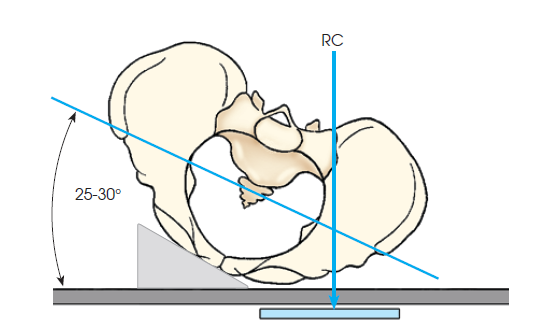
\includegraphics[width=0.7\linewidth]{imagenes/col54}
			\caption{}
			\label{fig:col54}
		\end{figure}
		
		
		\paragraph{Receptor de imagen}
		Centrado a la altura de la EIAS. Debe incluir la articulación sacroilíaca del lado en estudio con márgenes adecuados para su evaluación.
		
		\paragraph{Respiración}
		Suspendida durante la exposición.
		
		\subsubsection*{4. Anatomía Visible}
		
		Se visualiza la articulación sacroilíaca del lado más alejado del receptor (lado elevado). La oblicuidad proyecta la articulación de forma que solo se radiografía la porción más posterior de la misma; el rayo central no pasa tangencial a la parte anterior de la articulación. Esto es consecuencia de la oblicuidad propia de la articulación sacroilíaca, cuya orientación no es completamente coronal, sino que presenta un componente posterior y otro anterior.
		
		\subsubsection*{5. Criterios de Evaluación}
		
		\textbf{Posicionamiento correcto:} Espacio articular sacroilíaco abierto con mínima superposición del ilíaco y el sacro. La articulación debe quedar centrada en la radiografía.
		
		\textbf{Ausencia de rotación:} Oblicuidad de 25--30° correctamente mantenida, verificada por la apertura del espacio articular sacroilíaco sin exceso de superposición ósea.
		
		\textbf{Penetración y contraste:} Técnica adecuada al biotipo del paciente (básica, intermedia u homogeneizada), con visualización nítida de la interlínea articular sacroilíaca.
		
		\subsubsection*{6. Puntos Críticos}
		
		\textbf{Confusión de lado:} Recordar que el lado en estudio es el elevado (más alejado del RI). OPI demuestra la articulación derecha; OPD demuestra la izquierda.
		
		\textbf{Visualización parcial de la articulación:} Por la oblicuidad anatómica de la articulación sacroilíaca, solo se radiografía su porción posterior. No es posible obtener una imagen completa en una sola proyección oblicua, lo que limita la valoración. Este enfoque no es de uso común por esta razón.
		
		\textbf{Adaptaciones:} En pacientes con limitación para el decúbito supino, ajustar el apoyo con cuñas o almohadillas para mantener los 25--30° de oblicuidad.
		
		\textbf{Trucos:} Siempre explorar ambos lados para comparación bilateral. La radioprotección gonadal es de aplicación obligatoria en varones mediante colimación estrecha centrada en la articulación; en mujeres es técnicamente difícil de aplicar sin comprometer la región de interés.
		
		\subsection{Proyección PA Oblicua (OAD / OAI) --- Articulaciones Sacroilíacas}
		
		\subsubsection*{1. Identificación}
		
		\textbf{Tipo:} Proyección complementaria. Se realiza en ambas posiciones (OAD y OAI) para comparación bilateral.
		
		\textbf{Indicaciones clínicas principales:}
		\begin{itemize}
			\item Traumatismo de la articulación sacroilíaca.
			\item Pinzamiento, luxación o subluxación de la articulación sacroilíaca.
			\item Procesos patológicos de la articulación sacroilíaca.
		\end{itemize}
		
		\subsubsection*{2. Técnica Base}
		
		\textbf{Receptor de imagen:} 18x24 cm o 24x30 cm. Orientación \textbf{longitudinal} (vertical).
		
		\textbf{DFRI:} 100 cm.
		
		\textbf{Técnica:} Básica para pacientes de gran espesor; intermedia para pacientes estándar; homogeneizada para pacientes pediátricos o muy delgados.
		
		\textbf{Bucky:} Bucky de mesa con grilla.
		
		\subsubsection*{3. Posicionamiento}
		
		\paragraph{Paciente}
		Posición semiprona. El lado a estudiar queda más próximo al receptor de imagen. Se coloca almohada bajo la cabeza. El paciente se apoya sobre su antebrazo y flexiona la rodilla del lado elevado para estabilizar la posición.
		
		\paragraph{Región de interés}
		Se rota al paciente del lado de interés hacia la mesa unos 25--50°. Se ajusta el cuerpo de forma que su eje longitudinal sea paralelo al eje longitudinal de la mesa. Se centra el cuerpo de forma que un punto 2,5 cm medial a la EIAS más próxima al RI quede centrado sobre la línea media de la rejilla. OAD para demostrar la articulación derecha; OAI para demostrar la articulación izquierda.
		
		\paragraph{Rayo Central}
		Perpendicular al plano del receptor. Punto de entrada: \textbf{2,5 cm medial a la EIAS más próxima al RI}.

		
		\paragraph{Receptor de imagen}
		Centrado a la altura de la EIAS. Debe incluir la articulación sacroilíaca del lado en estudio.
		
		\paragraph{Respiración}
		Suspendida durante la exposición.
		
		\subsubsection*{4. Anatomía Visible}
		
		Se visualiza la articulación sacroilíaca del lado más próximo al receptor (lado en estudio). La colimación debe ser estrecha, limitada a la articulación sacroilíaca de interés.
		
		\subsubsection*{5. Criterios de Evaluación}
		
		\textbf{Posicionamiento correcto:} Articulación sacroilíaca del lado en estudio centrada en la radiografía, con apertura adecuada del espacio articular.
		
		\textbf{Ausencia de rotación:} Oblicuidad de 25--50° correctamente mantenida, verificada por la visualización del espacio articular sin superposición excesiva.
		
		\textbf{Penetración y contraste:} Técnica adecuada al biotipo del paciente (básica, intermedia u homogeneizada), con nitidez de la interlínea articular sacroilíaca.
		
		\subsubsection*{6. Puntos Críticos}
		
		\textbf{Confusión de lado:} En esta proyección el lado en estudio es el más próximo al RI (a diferencia de la AP oblicua). OAD demuestra la articulación derecha; OAI demuestra la izquierda.
		
		\textbf{Ángulo insuficiente o excesivo:} El rango de oblicuidad es amplio (25--50°); un ángulo inadecuado genera superposición del ilíaco sobre el sacro y cierre del espacio articular.
		
		\textbf{Adaptaciones:} En pacientes con dificultad para mantener la posición semiprona, utilizar cuñas o almohadillas bajo el tórax y la pelvis para sostener la oblicuidad requerida.
		
		\textbf{Trucos:} Siempre realizar ambas posiciones (OAD y OAI) para comparación bilateral. La colimación estrecha es obligatoria en todos los pacientes. Confirmar la oblicuidad palpando la posición de la EIAS antes de exponer.
		
		
		
		\onecolumn
		\clearpage
		
		\begin{figure}
			\centering
			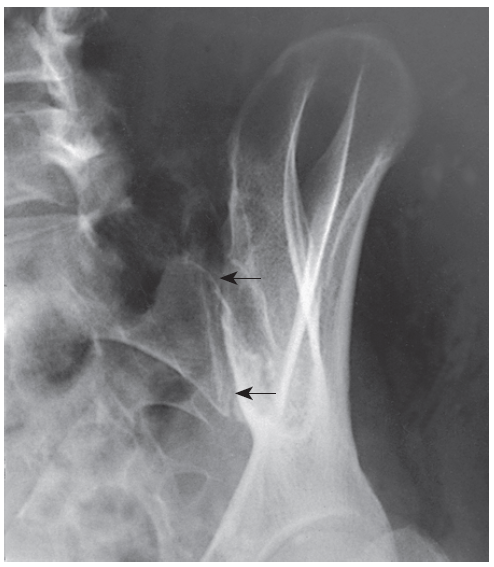
\includegraphics[width=0.7\linewidth]{imagenes/col55}
			\caption{OAI con 20° de angulación caudal}
			\label{fig:col55}
		\end{figure}
		
		
		
		\twocolumn
		\clearpage
		
		%----------------------------------------------------------
		%  Para agregar otro enfoque duplicá el bloque
		%  desde \subsection hasta \textbf{Trucos}
		%----------------------------------------------------------
		
		
%%%%%%%%%%%%%%%%%%%%%%%%%%%%%%%%%%%%%%%%%%%%%%%%%%%%%%%%%%%
%  SECCIÓN: Sacro y Cóccix
%  Archivo: secciones/sacro_coccix.tex
%  Sin preámbulo ni \begin{document} — lo maneja main.tex
	%%%%%%%%%%%%%%%%%%%%%%%%%%%%%%%%%%%%%%%%%%%%%%%%%%%%%%%%%%%
	
	\section{Columna Sacra}
	
	% ----------------------------------------------------------
	%  ENFOQUE 1: AP / PA AXIAL — SACRO
	% ----------------------------------------------------------
	
	\subsection{Proyección AP / PA Axial - Sacro}
	
	\subsubsection*{1. Identificación}
	
	\textbf{Tipo:} Proyección básica. La variante PA se emplea como alternativa posicional cuando la AP no es viable.
	
	\textbf{Indicaciones clínicas principales:}
	\begin{itemize}
		\item Patologías del sacro
		\item Fracturas o lesiones destructivas del sacro
		\item Evaluación de agujeros sacros, alas sacras y articulación lumbosacra
	\end{itemize}
	
	\subsubsection*{2. Técnica Base}
	
	\textbf{Receptor de imagen:} 24x30 cm.
	
	\textbf{DFRI:} 100 cm.
	
	\textbf{Técnica:} Intermedia. Permite equilibrar la visualización de las estructuras óseas del sacro con adecuado contraste.
	
	\textbf{Bucky:} Bucky de mesa con grilla.
	
	\subsubsection*{3. Posicionamiento}
	
	\paragraph{Paciente}
	\textbf{AP:} Decúbito supino. \textbf{PA:} Decúbito prono, empleada en pacientes con lesión dolorosa o enfermedad destructiva, sin pérdida de detalle diagnóstico respecto a la AP.
	En ambos casos el plano medio sagital perpendicular y centrado al receptor.
	
	% TODO: \usepackage{graphicx} required
	\begin{figure}[h]
		\centering
		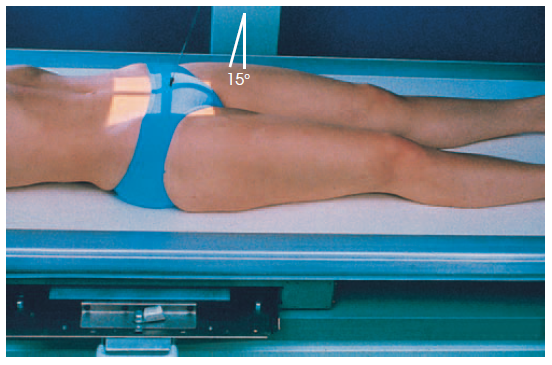
\includegraphics[width=0.7\linewidth]{imagenes/col56}
		\caption{}
		\label{fig:col56}
	\end{figure}
	
	
	\paragraph{Región de interés}
	Ambas EIAS equidistantes de la grilla para evitar rotación. Codos flexionados, brazos en posición simétrica bilateral cómoda. En supino, apoyo bajo las rodillas para reducir la lordosis lumbar y acercar el sacro al receptor. Los huesos deben estar tan próximos al receptor como sea posible.
	
	\paragraph{Rayo Central} - punto de entrada 5 cm por encima de la sínfisis púbica.\\
	\textbf{PA (prono):} 15° caudal - punto de entrada centrado sobre la curvatura sacra.\\
	La dirección se invierte al cambiar de posición para lograr el mismo efecto de desplegado del sacro.
	
	\paragraph{Receptor de imagen}
	Centrado de modo que incluya desde L5 hasta el cóccix.
	
	\paragraph{Respiración}
	Suspendida durante la exposición.
	
	\subsubsection*{4. Anatomía Visible}
	
	Sacro con su curvatura rectificada gracias a la angulación del RC. Se observan los agujeros sacros anteriores, las alas sacras simétricas, la articulación lumbosacra (L5--S1) y los huesos pubianos libres de superposición sobre el sacro. La angulación de 15° compensa la inclinación anterior del sacro, desplegando su curvatura.
	
	\subsubsection*{5. Criterios de Evaluación}
	
	\textbf{Posicionamiento correcto:} Sacro centrado, libre de acortamiento y con curvatura rectificada. Huesos pubianos no superpuestos al sacro. Ausencia de materia fecal superpuesta a la región de interés.
	
	\textbf{Ausencia de rotación:} Alas sacras simétricas en ambos lados. Ambas EIAS equidistantes de la línea media.
	
	\textbf{Penetración y contraste:} Escala de contraste corta que permita diferenciar las estructuras óseas del sacro.
	
	\subsubsection*{6. Puntos Críticos}
	
	\textbf{Angulación insuficiente del RC:} Provoca superposición del pubis sobre el sacro. El ángulo exacto (entre 10° y 20°) se ajusta según el promontorio y la morfología de caderas del paciente.
	
	\textbf{Confusión en la dirección de angulación al pasar a prono:} En PA la angulación es caudal, opuesta a la AP. Invertir la dirección es el error más frecuente al cambiar de posición.
	
	\textbf{Adaptaciones:} En pacientes con lesión dolorosa o enfermedad destructiva, emplear la variante PA (prono) con angulación caudal de 15°.
	
	\textbf{Trucos:} El sacro visto de perfil tiende a irse hacia adelante. La angulación del RC compensa esa inclinación natural; el ángulo exacto varía por paciente según el promontorio y la morfología de las caderas.
	
	
	\clearpage
	\onecolumn
	
	% TODO: \usepackage{graphicx} required
	\begin{figure}
		\centering
		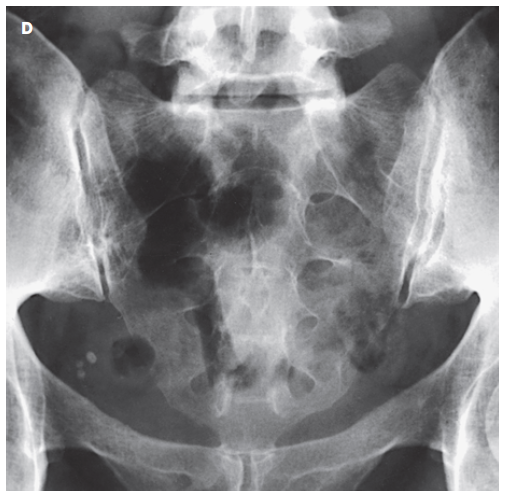
\includegraphics[width=0.7\linewidth]{imagenes/col57}
		\caption{AP de Sacro}
		\label{fig:col57}
	\end{figure}
			
	\twocolumn
	\clearpage
	
		\clearpage
	\onecolumn
	
	% TODO: \usepackage{graphicx} required
	\begin{figure}
		\centering
		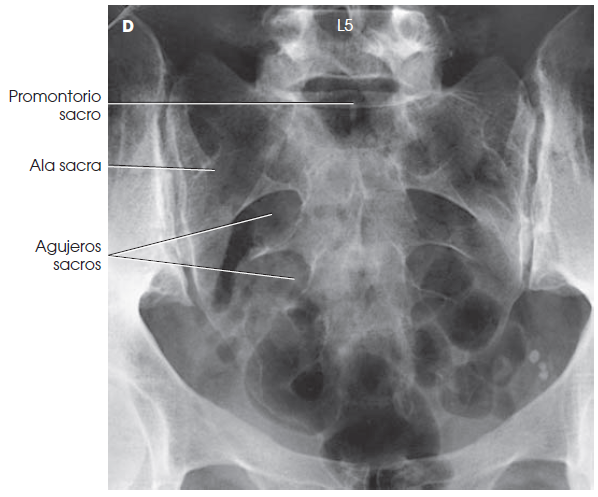
\includegraphics[width=0.7\linewidth]{imagenes/col58}
		\caption{AP de Sacro}
		\label{fig:col58}
	\end{figure}
	
	\twocolumn
	\clearpage
	% ----------------------------------------------------------
	%  ENFOQUE 2: AP / PA AXIAL — CÓCCIX
	% ----------------------------------------------------------
	
	\subsection{Proyección AP / PA Axial - Cóccix}
	
	\subsubsection*{1. Identificación}
	
	\textbf{Tipo:} Proyección básica. La variante PA se emplea como alternativa posicional cuando la AP no es viable.
	
	\textbf{Indicaciones clínicas principales:}
	\begin{itemize}
		\item Patologías del cóccix
		\item Traumatismos y fracturas coccígeas
		\item Evaluación de la alineación de los segmentos del cóccix
	\end{itemize}
	
	\subsubsection*{2. Técnica Base}
	
	\textbf{Receptor de imagen:} 18x24 cm.
	
	\textbf{DFRI:} 100 cm.
	
	\textbf{Técnica:} Intermedia.
	
	\textbf{Bucky:} Bucky de mesa con grilla.
	
	\subsubsection*{3. Posicionamiento}
	
	\paragraph{Paciente}
	\textbf{AP:} Decúbito supino. \textbf{PA:} Decúbito prono, empleada en pacientes con lesión dolorosa o enfermedad destructiva, sin pérdida de detalle diagnóstico respecto a la AP.
	En ambos casos el plano medio sagital perpendicular y centrado al receptor.
	
	% TODO: \usepackage{graphicx} required
	\begin{figure}[h]
		\centering
		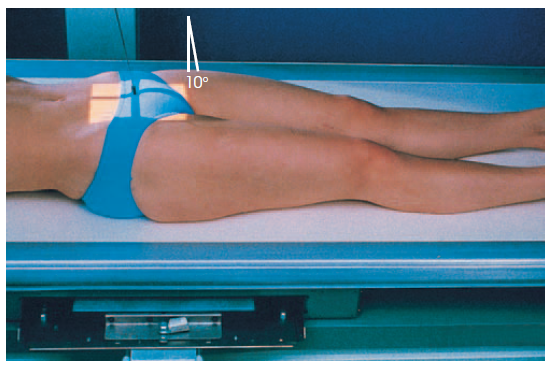
\includegraphics[width=0.7\linewidth]{imagenes/col59}
		\caption{}
		\label{fig:col59}
	\end{figure}
	
	
	\paragraph{Región de interés}
	Ambas EIAS equidistantes de la grilla. Codos flexionados, brazos en posición simétrica bilateral cómoda. En supino, apoyo bajo las rodillas. Los huesos deben estar tan próximos al receptor como sea posible.
	
	\paragraph{Rayo Central}
	\textbf{AP (supino):} 10° caudal - punto de entrada 5 cm por encima de la sínfisis púbica.\\
	\textbf{PA (prono):} 10° craneal - punto de entrada centrado sobre el cóccix prominente.\\
	La dirección se invierte al cambiar de posición para lograr el mismo efecto de desplegado de los segmentos coccígeos.
	
	\paragraph{Receptor de imagen}
	Centrado sobre la región coccígea. Colimación estrecha para mejorar la visualización y reducir la radiación dispersa. Incluir desde el sacro distal hasta el extremo del cóccix.
	
	\paragraph{Respiración}
	Suspendida durante la exposición.
	
	\subsubsection*{4. Anatomía Visible}
	
	Segmentos del cóccix sin superposición entre sí, centrados en la imagen, y articulación sacrococcígea. El cóccix presenta una curvatura cifótica opuesta a la del sacro, por lo que la angulación del RC en AP es caudal (inversa a la del sacro). La colimación estrecha mejora el contraste al reducir la radiación dispersa.
	
	\subsubsection*{5. Criterios de Evaluación}
	
	\textbf{Posicionamiento correcto:} Cóccix centrado y visible en su totalidad. Segmentos del cóccix no superpuestos. Colimación estrecha evidente en la imagen.
	
	\textbf{Ausencia de rotación:} Cóccix alineado sobre la línea media sin desviación lateral de sus segmentos.
	
	\textbf{Penetración y contraste:} Escala de contraste corta. La colimación estrecha mejora el contraste de la región.
	
	\subsubsection*{6. Puntos Críticos}
	
	\textbf{Confusión en la dirección de angulación respecto al sacro:} A diferencia del sacro (AP craneal), en el cóccix la AP es caudal por su curvatura cifótica opuesta. Es el error conceptual más frecuente al estudiar ambas regiones juntas.
	
	\textbf{Colimación inadecuada:} Una colimación amplia incrementa la radiación dispersa y degrada el contraste. Colimar estrictamente a la región de interés.
	
	\textbf{Adaptaciones:} En pacientes con lesión dolorosa, emplear la variante PA (prono) con angulación craneal de 10°.
	
	\textbf{Trucos:} El cóccix de perfil presenta una curvatura en cifosis, angulación contraria a la del sacro. La protección gonadal no puede colocarse en mujeres en esta proyección; en hombres se protegen las gónadas colocando el protector en los hombros.
	
	\onecolumn
	\clearpage
	
	% TODO: \usepackage{graphicx} required
	\begin{figure}
		\centering
		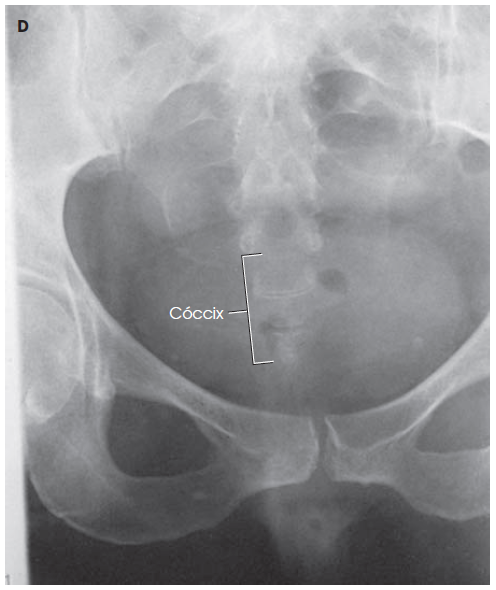
\includegraphics[width=0.7\linewidth]{imagenes/col60}
		\caption{AP Coxis}
		\label{fig:col60}
	\end{figure}
	
	
	\twocolumn
	\clearpage
	
	%----------------------------------------------------------
	%  Para agregar otro enfoque duplicá el bloque
	%  desde \subsection hasta \textbf{Trucos}
	%----------------------------------------------------------
	
	
%%%%%%%%%%%%%%%%%%%%%%%%%%%%%%%%%%%%%%%%%%%%%%%%%%%%%%%%%%%
%  SECCIÓN: Columna Lumbosacra — Sacro y Cóccix
%  Archivo: secciones/lateral_sacro_coccix.tex
%  Sin preámbulo ni \begin{document} — lo maneja main.tex
	%%%%%%%%%%%%%%%%%%%%%%%%%%%%%%%%%%%%%%%%%%%%%%%%%%%%%%%%%%%
	
	\section{Columna Coxis}
	
	\subsection{Proyección Lateral: Sacro y Cóccix}
	
	\subsubsection*{1. Identificación}
	
	\textbf{Tipo:} Proyección complementaria. Forma par con la proyección AP de sacro y cóccix.
	
	\textbf{Indicaciones clínicas principales:}
	\begin{itemize}
		\item Patologías del sacro
		\item Patologías del cóccix
	\end{itemize}
	
	\subsubsection*{2. Técnica Base}
	
	\textbf{Receptor de imagen (sacro):} 24$\times$30 cm, centrado en la línea media del sacro.
	
	\textbf{Receptor de imagen (cóccix):} 18$\times$24 cm, centrado en la línea media del cóccix.
	
	\textbf{DFRI:} 100 cm.
	
	\textbf{Técnica:} Intermedia.
	
	\textbf{Bucky:} Sí.
	
	\subsubsection*{3. Posicionamiento}
	
	\paragraph{Paciente}
	Paciente en decúbito lateral, girado hacia el lado indicado. Flexionar caderas y rodillas en una posición cómoda. Ajustar brazos en una posición cómoda. Colocar soporte bajo el cuerpo para situar el eje longitudinal de la columna horizontal. Ajustar pelvis y hombros para obtener una posición lateral verdadera.
	
	% TODO: \usepackage{graphicx} required
	\begin{figure}[h]
		\centering
		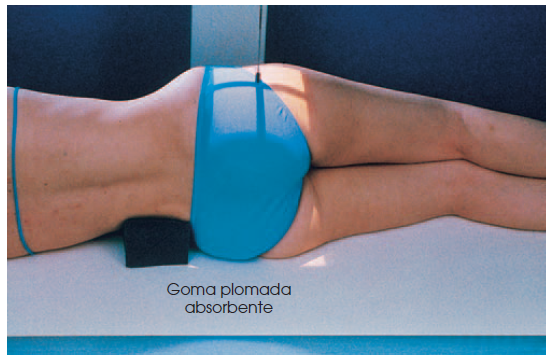
\includegraphics[width=0.7\linewidth]{imagenes/col61}
		\caption{Lateral de Coxis}
		\label{fig:col61}
	\end{figure}
	
	% TODO: \usepackage{graphicx} required
	\begin{figure}[h]
		\centering
		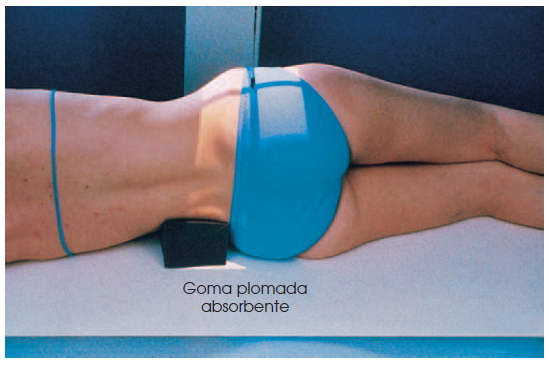
\includegraphics[width=0.7\linewidth]{imagenes/col62}
		\caption{Lateral de Sacro}
		\label{fig:col62}
	\end{figure}
	
	
	\paragraph{Región de interés}
	La posición exacta del sacro depende de la curvatura pélvica del paciente. Los márgenes posteriores de los isquiones y los iliacos deben quedar casi superpuestos entre sí. Colimación estrecha sobre la región de interés.
	
	\paragraph{Rayo Central — Sacro}
	RC perpendicular al plano del receptor. Punto de entrada: \textbf{EIAS, dirigido 9 cm posterior a la misma}.
	
	\paragraph{Rayo Central — Cóccix}
	RC perpendicular al plano del receptor. Punto de entrada: \textbf{9 cm posterior y 5 cm inferior a la EIAS}.
	
	\paragraph{Respiración}
	Suspendida durante la exposición.
	
	\subsubsection*{4. Anatomía Visible}
	
	Sacro y cóccix en proyección lateral. La superposición de los márgenes posteriores de los isquiones e iliacos entre sí confirma el posicionamiento lateral verdadero. La curvatura natural del sacro queda demostrada sin rotación pélvica.
	
	\subsubsection*{5. Criterios de Evaluación}
	
	\textbf{Posicionamiento correcto:} Márgenes posteriores de los isquiones y los iliacos casi superpuestos entre sí; eje longitudinal de la columna horizontal al receptor.
	
	\textbf{Ausencia de rotación:} Superposición simétrica de los elementos posteriores de la pelvis; pelvis y hombros en lateral verdadero sin inclinación.
	
	\textbf{Penetración y contraste:} Técnica intermedia que permita visualizar el sacro y el cóccix con densidad adecuada, diferenciando las estructuras óseas del tejido blando circundante.
	
	\subsubsection*{6. Puntos Críticos}
	
	\textbf{Rotación pélvica:} Genera superposición asimétrica de los isquiones e iliacos, distorsionando la imagen del sacro y el cóccix; corregir ajustando pelvis y hombros a lateral verdadero.
	
	\textbf{Eje de columna no horizontal:} Si el soporte bajo el cuerpo es insuficiente, la columna queda inclinada y el RC no incide perpendicularmente sobre la región; verificar la horizontalidad antes de la exposición.
	
	\textbf{Adaptaciones:} En pacientes con limitaciones de movilidad o dolor agudo, ajustar el grado de flexión de caderas y rodillas según tolerancia, manteniendo la prioridad de lograr el lateral verdadero.
	
	\textbf{Trucos:} La EIAS es el repere principal y es fácilmente palpable con el paciente en decúbito lateral. Para el sacro, medir 9 cm posterior a la EIAS; para el cóccix, combinar 9 cm posterior y 5 cm inferior. Solicitar colimación estrecha para reducir radiación dispersa y mejorar el contraste en ambas estructuras.
	
	
	\onecolumn
	\clearpage
	
	% TODO: \usepackage{graphicx} required
	\begin{figure}
		\centering
		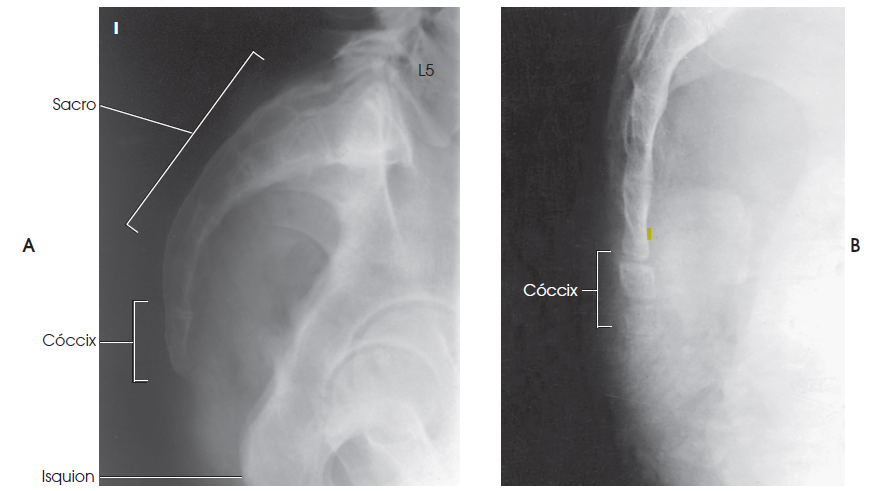
\includegraphics[width=1\linewidth]{imagenes/col63}
		\caption{\textbf{A}. Proyección lateral del sacro. \textbf{B}. Proyección lateral del cóccix.
		}
		\label{fig:col63}
	\end{figure}
		
	
	\twocolumn
	\clearpage
	
	%----------------------------------------------------------
	%  Para agregar otro enfoque duplicá el bloque
	%  desde \subsection hasta \textbf{Trucos}
	%----------------------------------------------------------
	
	
%%%%%%%%%%%%%%%%%%%%%%%%%%%%%%%%%%%%%%%%%%%%%%%%%%%%%%%%%%%
%  SECCIÓN: Diagnóstico por Imágenes — Escoliosis
%  Archivo: secciones/dc_escoliosis.tex
%  Sin preámbulo ni \begin{document} — lo maneja main.tex
	%%%%%%%%%%%%%%%%%%%%%%%%%%%%%%%%%%%%%%%%%%%%%%%%%%%%%%%%%%%
	
	\section{Columna - Escoliosis}
	
	%----------------------------------------------------------
	\subsection{Definición y Características Generales}
	
	\subsubsection*{Concepto}
	
	La escoliosis es la desviación de la columna vertebral con deformidad tridimensional. La deformidad predominante se localiza en el \textbf{plano coronal} (desviación derecha–izquierda), con un componente rotacional asociado que puede afectar la cifosis dorsal y la lordosis lumbar. Para ser considerada escoliosis, la angulación debe superar los \textbf{10°}.
	
	\subsubsection*{Planos de la Columna}
	
	\textbf{Plano sagital:} contiene las curvaturas fisiológicas normales.
	\begin{itemize}
		\item Lordosis cervical y lumbar
		\item Cifosis torácica y sacra
	\end{itemize}
	
	\textbf{Plano coronal:} toda curvatura en este plano es \textbf{patológica} (desviación lateral derecha–izquierda o izquierda–derecha).
	
	
	\begin{figure}[h]
		\centering
		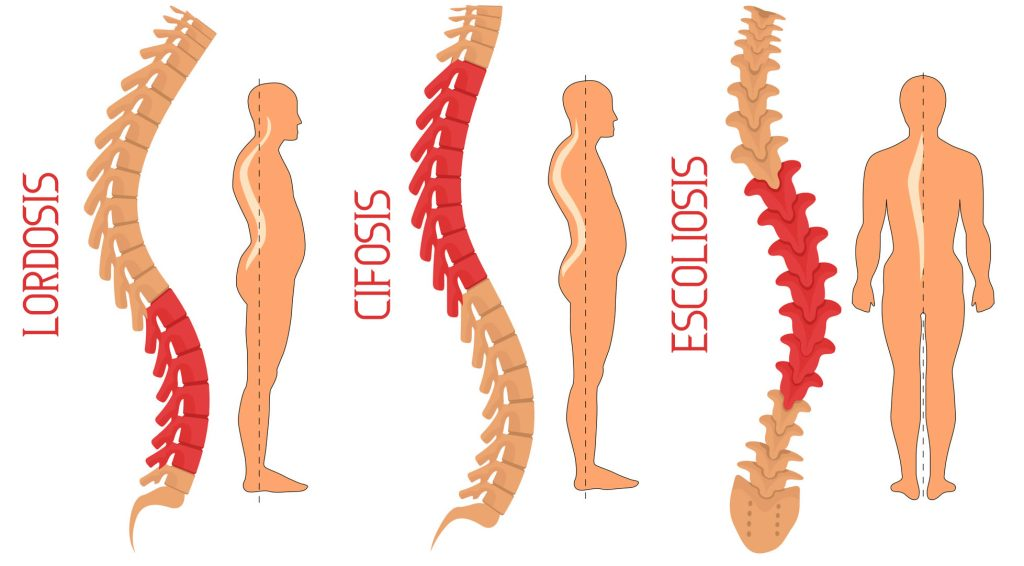
\includegraphics[width=0.7\linewidth]{imagenes/col64}
		\caption{}
		\label{fig:col64}
	\end{figure}
	
	
	%----------------------------------------------------------
	\subsection{Vértebras de Referencia en Escoliosis}
	
		% TODO: \usepackage{graphicx} required
	\begin{figure}[h]
		\centering
		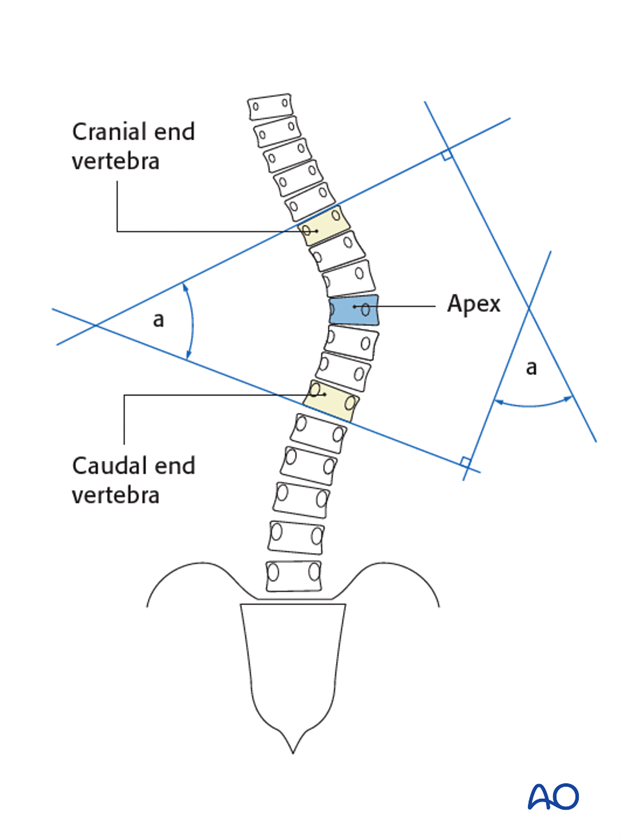
\includegraphics[width=0.7\linewidth]{imagenes/col67}
		\caption{}
		\label{fig:col65}
	\end{figure}
	
	
	\subsubsection*{Vértebra Proximal (Extremo Superior)}
	Es la vértebra más superior de la curvatura. Su superficie superior gira en sentido máximo hacia la concavidad de la curva. Es la primera vértebra en manifestarse en la curvatura.
	
	\subsubsection*{Vértebra Distal (Terminal)}
	Es la vértebra más inferior de la curvatura. Su superficie inferior gira en sentido máximo hacia la concavidad de la curva. Es la última vértebra en manifestarse en la curvatura.
	
	\subsubsection*{Vértebra Ápex (Apical)}
	Es la vértebra más desviada del eje vertical del paciente. Es también la más rotada, lo que determina su mayor desplazamiento lateral. Corresponde al punto máximo de la curvatura.
	
	
	%----------------------------------------------------------
	\subsection{Clasificación de las Curvas}
	

	
	\subsubsection*{Curva Primaria}
	La curva principal de la escoliosis. Presenta mayor rotación y desviación de los cuerpos vertebrales. Es la menos flexible: al colocar un cajón bajo el pie del lado convexo, esta curva no se modifica. Corresponde siempre a la curva con \textbf{mayor ángulo de Cobb}.
	
	\subsubsection*{Curva Secundaria (Compensadora)}
	Son las curvas que el cuerpo genera para compensar la curva primaria, en dirección opuesta. Son menos acentuadas y más flexibles. Siempre están presentes junto a la curva primaria. El ángulo de la curva compensadora es \textbf{menor} que el de la curva primaria.
	
	\textbf{Ejemplo:} curva primaria dorsal + curva compensadora lumbar.
	
	\subsubsection*{Curva Estructural}
	La curva está fija en ese segmento espinal. No puede corregirse por completo en radiografías con el paciente en decúbito dorsal ni en flexión lateral. Se perdió flexibilidad en la columna.
	
	\subsubsection*{Curva No Estructural}
	No tiene rotación fija ni angulación lateral permanente. Puede corregirse completamente por tracción o flexión lateral. Corresponde a escoliosis postural o por mala posición; al colocar un cajoncito, esta curva mejora.
	
	\onecolumn
	
	\begin{figure}
		\centering
		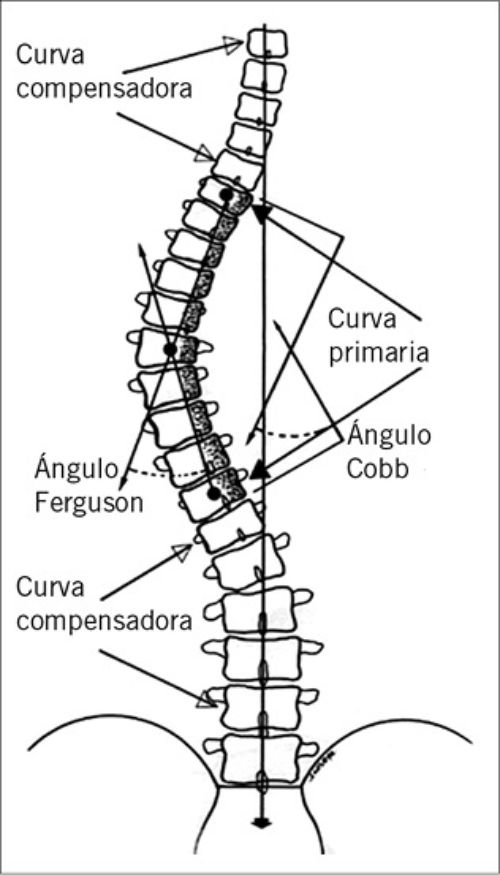
\includegraphics[width=0.6\linewidth]{imagenes/col65}
		\caption{}
		\label{fig:col65}
	\end{figure}
	
	\twocolumn	
	%----------------------------------------------------------
	\clearpage
	\subsection{Ángulo de Cobb}
	
	\subsubsection*{Técnica de Medición}
	
	\paragraph{Paso 1}
	Trazar una línea paralela al \textbf{platillo superior} de la vértebra límite superior de la curvatura.
	
	\paragraph{Paso 2}
	Trazar una línea paralela al \textbf{platillo inferior} de la vértebra límite inferior de la curvatura.
	
	\paragraph{Paso 3}
	Trazar perpendiculares a ambas líneas y medir el ángulo formado entre ellas.
	
	\paragraph{Referencia alternativa}
	Si los platillos no son identificables en la radiografía, se toman como referencia los \textbf{bordes de los pedículos}.
	
	\subsubsection*{Interpretación Clínica}
	
	\textbf{Menos de 20°:} observación y control periódico.
	
	\textbf{Entre 20° y 40°:} tratamiento ortopédico.
	
	\textbf{Mayor de 50°:} indicación quirúrgica.
	
	\subsubsection*{Utilidad del Ángulo de Cobb}
	Cuantifica la desviación vertebral en el plano coronal. Permite diferenciar la \textbf{curva mayor} (mayor ángulo) de las \textbf{curvas menores} (ángulo menor). Las curvaturas menores tienden a compensar la curvatura mayor. Siempre se visualizan al menos dos curvaturas: una escoliótica y una compensatoria.
	
	\clearpage
	\onecolumn
	
	% TODO: \usepackage{graphicx} required
	\begin{figure}
		\centering
		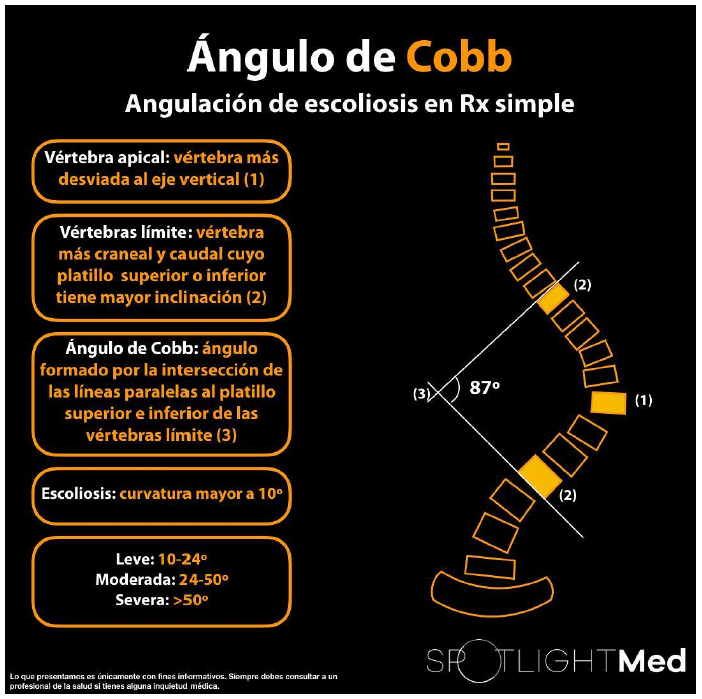
\includegraphics[width=0.7\linewidth]{imagenes/col66}
		\caption{}
		\label{fig:col66}
	\end{figure}
	
	
	\twocolumn
	\clearpage
	
	%----------------------------------------------------------
\subsection{Signo de Risser}

\subsubsection*{Definición}
Indicador radiográfico de \textbf{madurez esquelética} desarrollado por el Dr. Joseph C. Risser en 1958. Evalúa el grado de osificación de la \textbf{apófisis ilíaca (cresta ilíaca)} en radiografías de pelvis. La osificación de las apófisis ilíacas ocurre de manera paralela a la de las apófisis vertebrales, permitiendo estimar el potencial de crecimiento espinal restante.

\subsubsection*{Proceso de Osificación}
La osificación comienza en la región \textbf{anterolateral} de la cresta ilíaca (cerca de la espina ilíaca anterosuperior), avanza medialmente hacia la espina ilíaca posterosuperior y finalmente se fusiona en dirección medial a lateral.

\subsubsection*{Escala de Clasificación (0--5)}

\textbf{Risser 0:} Sin osificación visible. Crecimiento significativo restante. Alto riesgo de progresión de escoliosis. Etapa prepuberal o pubertad temprana.

\textbf{Risser 1:} Osificación del 25\% de la cresta ilíaca. Potencial de crecimiento considerable. Etapa prepuberal o pubertad temprana.

\textbf{Risser 2:} Osificación del 50\%. Potencial de crecimiento moderado. Antes o durante el pico de crecimiento.

\textbf{Risser 3:} Osificación del 75\%. Potencial limitado. Etapa de desaceleración del crecimiento.

\textbf{Risser 4:} Osificación completa (100\%) sin fusión. Potencial mínimo. Casi cesación del crecimiento.

\textbf{Risser 5:} Fusión completa de la apófisis con el ilion. Madurez esquelética completa. Sin crecimiento restante.

\subsubsection*{Importancia Clínica}

\textbf{Predicción de progresión:} Pacientes con Risser 0--2 presentan mayor riesgo de progresión de la curvatura escoliótica y requieren seguimiento más intensivo.

\textbf{Decisión terapéutica:} El corsé ortopédico es más efectivo en grados bajos (0--2). A mayor madurez, mayor probabilidad de indicación quirúrgica. Pacientes con Risser 4--5 requieren menos seguimiento activo.

\subsubsection*{Importancia Técnica --- Colimación}
Al dejar el colimador abierto en la radiografía panorámica de columna, se incluyen la pelvis y las crestas ilíacas en una sola toma. Esto \textbf{evita una radiografía adicional de pelvis} y reduce la dosis de radiación al paciente.

\subsubsection*{Técnica Radiológica}
Se evalúa en la \textbf{radiografía AP de pelvis}, incluida en el estudio de columna completa, con el paciente en bipedestación. Se requiere visualización completa de \textbf{ambas crestas ilíacas} y evaluación bilateral del porcentaje de osificación y de la fusión apofisaria.
	
	\onecolumn
	
	
	% TODO: \usepackage{graphicx} required
	\begin{figure}
		\centering
		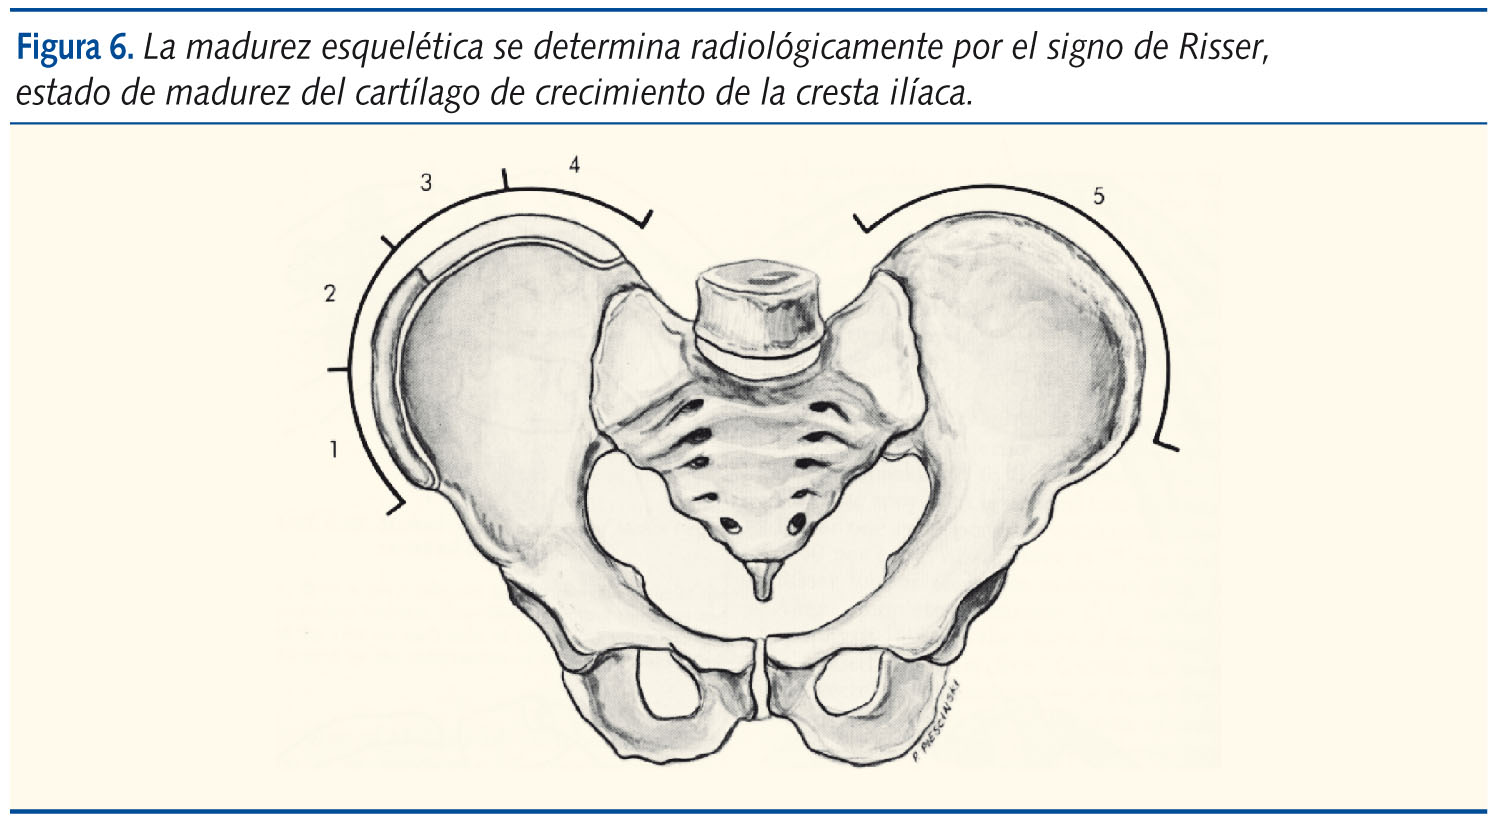
\includegraphics[width=0.8\linewidth]{imagenes/col71}
		\caption{}
		\label{fig:col70}
	\end{figure}
	
	\begin{figure}
		\centering
		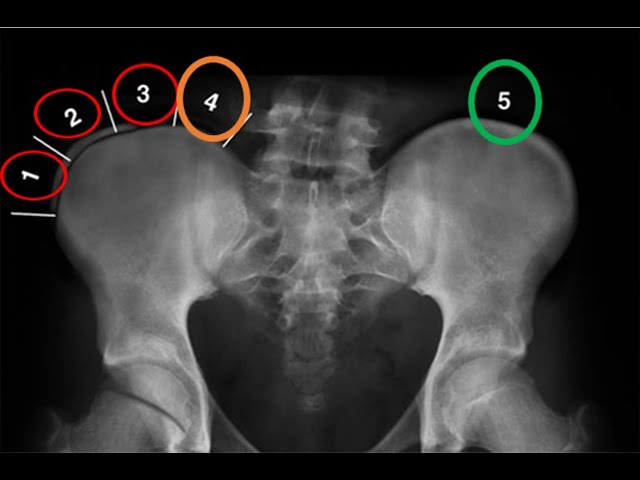
\includegraphics[width=0.8\linewidth]{imagenes/col70}
		\caption{}
		\label{fig:col70}
	\end{figure}
	
	
	
	
	\twocolumn
	\clearpage
	%----------------------------------------------------------
	\subsection{Estudio Radiológico de la Escoliosis}
	
	\subsubsection*{Objetivos del Estudio}
	\begin{itemize}
		\item Visualizar las deformidades de los ejes de la columna vertebral.
		\item Cuantificar el grado de desviación mediante el ángulo de Cobb.
		\item Estimar el grado de madurez ósea del paciente (Signo de Risser).
	\end{itemize}
	
	\subsubsection*{Proyecciones Indicadas}
	\begin{itemize}
		\item Proyección panorámica de columna AP (PA) — frente.
		\item Proyección panorámica lateral de columna.
	\end{itemize}
	
	\subsubsection*{Elección del Perfil}
	La elección del perfil depende de la curvatura del paciente. Se coloca siempre la \textbf{concavidad de la curvatura hacia el lado del tubo}.
	
	\textbf{Ejemplo:} si la curvatura tiene concavidad izquierda → perfil derecho.
	
	\subsubsection*{Posición del Paciente — Aspectos Críticos}
	
	\textbf{Bipedestación:} el paciente debe estar de pie de forma \textbf{obligatoria}. La radiografía en carga refleja la posición anatómica real.
	
	\textbf{Descalzo:} el paciente debe estar sin calzado de forma \textbf{fundamental}. El calzado (especialmente con tacones o desgaste desigual) puede generar un falso diagnóstico al alterar la postura basal.
	
	\textbf{Distribución del peso:} el peso corporal debe estar distribuido equitativamente en ambos pies, para valorar la columna con la carga activa real del paciente.
	
	
	
	%----------------------------------------------------------
	%  Fin de sección dc_escoliosis.tex
	%----------------------------------------------------------
	\clearpage
	
%%%%%%%%%%%%%%%%%%%%%%%%%%%%%%%%%%%%%%%%%%%%%%%%%%%%%%%%%%%
%  SECCIÓN: Columna Vertebral — Proyecciones Panorámicas
%  Archivo: secciones/columna_panoramica.tex
%  Sin preámbulo ni \begin{document} — lo maneja main.tex
	%%%%%%%%%%%%%%%%%%%%%%%%%%%%%%%%%%%%%%%%%%%%%%%%%%%%%%%%%%%
	
	\section{Columna Escoliosis}
	
	\subsection{Panorámica de Columna AP/PA - Frente}
	
	\subsubsection*{1. Identificación}
	
	\textbf{Tipo:} Proyección básica. Forma par con la proyección panorámica de columna en perfil.
	
	\textbf{Indicaciones clínicas principales:}
	\begin{itemize}
		\item Escoliosis: evaluación de grado e intensidad de la curvatura.
		\item Caracterización de deformidades de los ejes de la columna vertebral.
		\item Estimación del grado de madurez esquelética (índice de Risser) como factor pronóstico para el manejo médico o quirúrgico.
	\end{itemize}
	
	\subsubsection*{2. Técnica Base}
	
	\textbf{Receptor de imagen:} 35x43 cm. Orientación \textbf{longitudinal} (vertical). Borde inferior ubicado 3--5 cm por debajo de la cresta ilíaca.
	
	\textbf{DFRI:} 180--200 cm (mínimo 150 cm). Se requiere mayor SID cuando se utiliza un receptor de mayor tamaño, a fin de obtener la colimación requerida.
	
	\textbf{Técnica:} Homogenizada en paciente pediátrico (80\,kVp --- 40\,mAs; perfil: 80\,kVp --- 80\,mAs o 100\,kVp --- 100\,mAs). Técnica intermedia en adulto.
	
	\textbf{Bucky:} Bucky vertical con grilla.
	
	\subsubsection*{3. Posicionamiento}
	
	\paragraph{Paciente}
	De pie (bipedestación), descalzo, con el peso distribuido equitativamente sobre ambos miembros inferiores. Se recomienda la posición PA (pecho pegado al Bucky vertical) por razones de radioprotección. En pacientes pediátricos se prefiere AP, dado que los niños tienden a moverse y es más difícil mantenerlos en PA.
	
	% TODO: \usepackage{graphicx} required
	\begin{figure}[h]
		\centering
		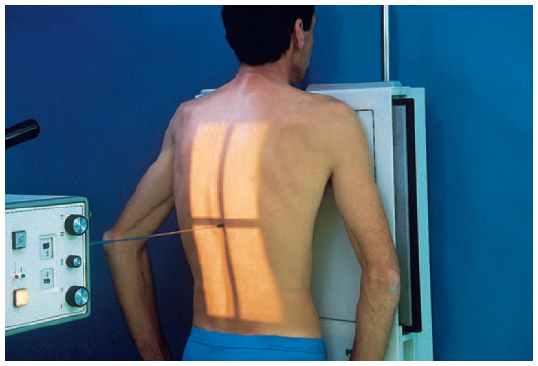
\includegraphics[width=0.7\linewidth]{imagenes/col76}
		\caption{}
		\label{fig:col76}
	\end{figure}
	
	
	\paragraph{Región de interés}
	Brazos a los costados del cuerpo. Verificar ausencia de rotación del torso y de la pelvis. Se toma referencia desde el plano medio sagital, 4 dedos lateralmente. Nota: la escoliosis puede generar rotación vertebral inherente, por lo que cierta rotación es inevitable y esperada.
	
	\paragraph{Rayo Central}
	Perpendicular al plano del receptor. Punto de entrada: \textbf{punto medio del receptor de imagen}.
	
	\paragraph{Receptor de imagen}
	Centrado de modo que el borde inferior quede 3-5 cm por debajo de la cresta ilíaca. Debe incluir vértebras torácicas, lumbares y quirúrgicas, y la totalidad de las crestas ilíacas (especialmente en adolescentes). Colimación a los cuatro lados; no se recomienda colimación estrecha, ya que es necesario evaluar las deformidades de costillas y pelvis adyacentes.
	
	\paragraph{Respiración}
	Suspendida al final de una espiración: se indica al paciente que inhale y luego aguante la respiración.
	
	\subsubsection*{4. Anatomía Visible}
	
	Vértebras torácicas, lumbares y quirúrgicas en proyección frontal. Totalidad de las crestas ilíacas, con al menos 2.5 cm visibles por encima de su borde superior en pacientes adolescentes, como indicador del índice de Risser. Regiones costales adyacentes y pelvis en sus márgenes. Puede evidenciarse rotación vertebral asociada a la curvatura escoliótica, lo cual es un hallazgo esperado y no un error técnico.
	
	\subsubsection*{5. Criterios de Evaluación}
	
	\textbf{Posicionamiento correcto:} Visualización de al menos 2.5 cm de crestas ilíacas por encima de su borde superior en pacientes adolescentes. Inclusión completa de vértebras torácicas, lumbares y quirúrgicas en un solo receptor.
	
	\textbf{Ausencia de rotación:} Simetría del torso y pelvis en la medida en que la patología lo permita. Se acepta rotación inherente a la escoliosis.
	
	\textbf{Penetración y contraste:} Adecuada visualización de los cuerpos vertebrales y espacios intervertebrales en toda la extensión de la columna. La técnica homogeneizada (niño) o intermedia (adulto) debe garantizar uniformidad de densidad en regiones torácica y lumbar simultáneamente.
	
	\subsubsection*{6. Puntos Críticos}
	
	\textbf{Colimación excesivamente estrecha:} Impide la evaluación de costillas adyacentes y pelvis, perdiendo información clínica relevante para la clasificación de la deformidad. Colimar a los cuatro lados sin estrechar lateralmente.
	
	\textbf{Omisión de crestas ilíacas:} En adolescentes, no visualizar al menos 2.5 cm de crestas ilíacas impide determinar el índice de Risser, dato esencial para la decisión médico-quirúrgica. Ajustar el borde inferior del receptor a 3--5 cm por debajo de la cresta.
	
	\textbf{Adaptaciones:} Si las estructuras no entran en el receptor, priorizar la región donde el paciente presenta la curvatura. En pediátricos que no cooperan en PA, realizar en AP.
	
	\textbf{Trucos:} La imagen se invierte horizontalmente al revelar; marcar a la derecha (queda del mismo lado que el corazón). Según criterio Pereira: la marca queda del lado izquierdo y el perfil no se marca. El mayor grado de madurez ósea implica menor posibilidad de corrección sin intervención quirúrgica.
	
	\clearpage
	\onecolumn
	
	% TODO: \usepackage{graphicx} required
	\begin{figure}
		\centering
		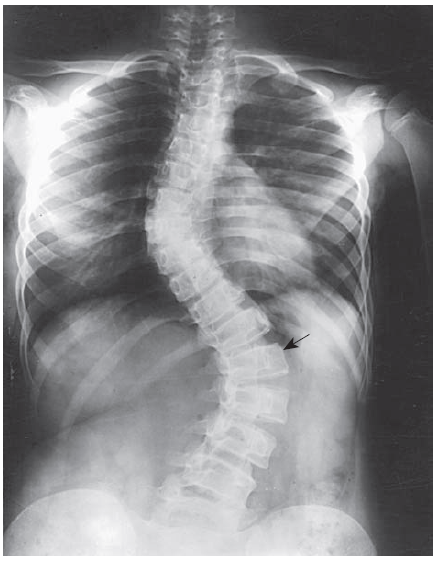
\includegraphics[width=0.7\linewidth]{imagenes/col75}
		\caption{}
		\label{fig:col75}
	\end{figure}
	
	
	
	\clearpage
	\twocolumn
	
	%----------------------------------------------------------
	%  Para agregar otro enfoque duplicá el bloque
	%  desde \subsection hasta \textbf{Trucos}
	%---------------------------------------------------------
	
	
%%%%%%%%%%%%%%%%%%%%%%%%%%%%%%%%%%%%%%%%%%%%%%%%%%%%%%%%%%%
%  SECCIÓN: Columna Vertebral — Proyecciones Panorámicas
%  Archivo: secciones/columna_panoramica_lateral.tex
%  Sin preámbulo ni \begin{document} — lo maneja main.tex
	%%%%%%%%%%%%%%%%%%%%%%%%%%%%%%%%%%%%%%%%%%%%%%%%%%%%%%%%%%%
	
	\section{Columna Escoliosis}
	
	\subsection{Panorámica Lateral de Columna (Niño)}
	
	\subsubsection*{1. Identificación}
	
	\textbf{Tipo:} Proyección complementaria. Forma par con la proyección panorámica AP/PA de frente.
	
	\textbf{Indicaciones clínicas principales:}
	\begin{itemize}
		\item Escoliosis: evaluación en el plano sagital.
		\item Espondilolistesis.
		\item Valoración del grado de cifosis y lordosis.
	\end{itemize}
	
	\subsubsection*{2. Técnica Base}
	
	\textbf{Receptor de imagen:} 35x43 cm. Orientación \textbf{longitudinal} (vertical), con respecto al eje mayor de la región. Borde superior a nivel de C7; borde inferior 3--5 cm por debajo de las crestas ilíacas.
	
	\textbf{DFRI:} 180--200 cm (mínimo 150 cm).
	
	\textbf{Técnica:} Homogenizada. Los mAs se duplican respecto al frente para compensar el mayor espesor lateral.
	
	\textbf{Bucky:} Bucky vertical con grilla.
	
	\subsubsection*{3. Posicionamiento}
	
	\paragraph{Paciente}
	De pie (bipedestación), descalzo. Lateralizado al Bucky. El lado \textbf{convexo} de la curva se apoya contra el receptor. Se aplica marcador D o I acorde a hacia donde esté la curvatura.
	
	\paragraph{Región de interés}
	Posición lateral verdadera de pelvis y torso. Brazos llevados hacia adelante a 45°, posición más cómoda para el paciente. Esta posición de brazos evita la superposición sobre la columna y no falsea la lordosis.
	
	\paragraph{Rayo Central}
	Perpendicular al plano del receptor. Punto de entrada: \textbf{4 dedos por dentro del reborde cutáneo posterior}, dirigido al punto medio del receptor de imagen.
	
	\paragraph{Receptor de imagen}
	Borde superior a nivel de C7, dirección caudal. Borde inferior 3--5 cm por debajo de las crestas ilíacas. Debe incluir la región de C7 hacia abajo y al menos 2.5 cm de crestas ilíacas.
	
	\paragraph{Respiración}
	Suspendida al final de la espiración.
	
	\subsubsection*{4. Anatomía Visible}
	
	Vértebras torácicas y lumbares en proyección lateral. Crestas ilíacas (al menos 2.5 cm). En pacientes con escoliosis los arcos costales no estarán bien superpuestos; esto es un hallazgo esperado y no un error técnico, ya que las vértebras de la curvatura pueden estar rotadas, ocasionando distorsión de la caja torácica.
	
	\subsubsection*{5. Criterios de Evaluación}
	
	\textbf{Posicionamiento correcto:} Visualización de C7 hacia abajo con inclusión de al menos 2.5 cm de crestas ilíacas. Posición lateral verdadera de pelvis y torso.
	
	\textbf{Ausencia de rotación:} En lo posible, plano coronal perpendicular al receptor. Se acepta rotación residual inherente a la curvatura escoliótica; los arcos costales no superpuestos en escoliosis dorsal son esperados.
	
	\textbf{Penetración y contraste:} Adecuada visualización de cuerpos vertebrales, espacios intervertebrales y platillos vertebrales en toda la extensión toracolumbar con técnica homogeneizada.
	
	\subsubsection*{6. Puntos Críticos}
	
	\textbf{Elección incorrecta del lado de apoyo:} Siempre realizar primero el frente panorámico para identificar la curvatura. El lado \textbf{cóncavo} debe quedar orientado hacia el tubo: la divergencia cónica del haz hace que los rayos pasen tangenciales a los espacios discales y tiendan a abrirlos. Si se coloca la convexidad hacia el tubo, los espacios articulares se cierran. Ejemplo: concavidad izquierda → perfil derecho (lado izquierdo hacia el tubo).
	
	\textbf{Brazos en posición incorrecta:} Llevar los brazos hacia atrás los superpone a la columna dorsal. Siempre hacia adelante a 45°.
	
	\textbf{Adaptaciones:} En pacientes pediátricos la posición a 45° de brazos resulta más cómoda y reduce el movimiento. Registrar siempre el lado de apoyo utilizado.
	
	\textbf{Trucos:} Consultar siempre la proyección de frente antes de posicionar al paciente para el perfil. La posición de brazos hacia adelante además evita falsear la lordosis lumbar.
	
	
	\onecolumn
	\clearpage
	
	% TODO: \usepackage{graphicx} required
	\begin{figure}
		\centering
		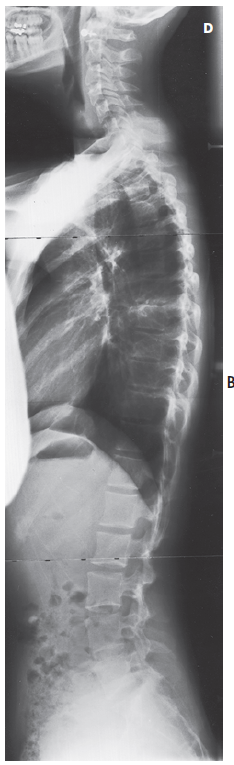
\includegraphics[width=0.3\linewidth]{imagenes/col77}
		\caption{}
		\label{fig:col77}
	\end{figure}
		
	\twocolumn
	\clearpage
	
	%----------------------------------------------------------
	%  Para agregar otro enfoque duplicá el bloque
	%  desde \subsection hasta \textbf{Trucos}
	%----------------------------------------------------------
	
	\subsection{Panorámica Lateral de Columna (Eddy) - Técnica con Doble Exposición}
	
	\subsubsection*{1. Identificación}
	
	\textbf{Tipo:} Proyección complementaria. Forma par con la proyección panorámica AP/PA de frente.
	
	\textbf{Indicaciones clínicas principales:}
	\begin{itemize}
		\item Escoliosis: evaluación en el plano sagital.
		\item Espondilolistesis.
		\item Valoración del grado de cifosis y lordosis.
	\end{itemize}
	
	\subsubsection*{2. Técnica Base}
	
	\textbf{Receptor de imagen:} 35x43 cm. Orientación \textbf{longitudinal} (vertical). Borde superior a nivel de C7; borde inferior 3--5 cm por debajo de las crestas ilíacas.
	
	\textbf{DFRI:} 180--200 cm en ambas exposiciones, para que las dos imágenes queden con igual magnificación y sean comparables.
	
	\textbf{Técnica:} Intermedia. Se realizan \textbf{dos exposiciones} sobre el mismo receptor: la primera centrada en región torácica (C7 hacia abajo, en inspiración) y la segunda centrada en región lumbar (a nivel de crestas ilíacas, en espiración).
	
	\textbf{Bucky:} Bucky vertical con grilla.
	
	\subsubsection*{3. Posicionamiento}
	
	\paragraph{Paciente}
	De pie (bipedestación), descalzo. PMS paralelo al receptor. Lateralizado al Bucky. El lado \textbf{convexo} de la curva primaria se apoya contra el receptor. Se aplica marcador D o I acorde a la curvatura.
	
	% TODO: \usepackage{graphicx} required
	\begin{figure}[h]
		\centering
		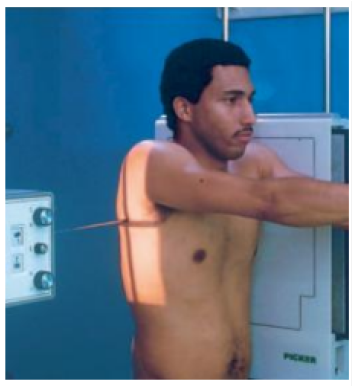
\includegraphics[width=0.7\linewidth]{imagenes/col78}
		\caption{}
		\label{fig:col78}
	\end{figure}
	
	% TODO: \usepackage{graphicx} required
	\begin{figure}[h]
		\centering
		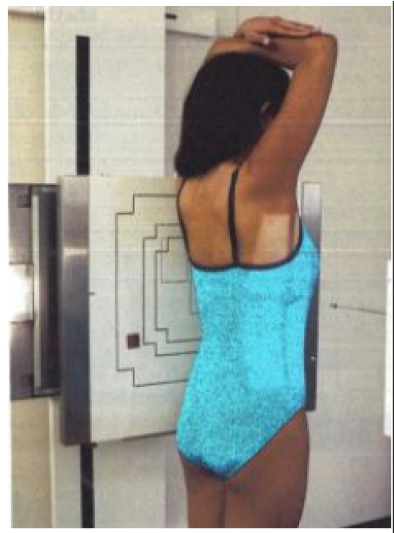
\includegraphics[width=0.7\linewidth]{imagenes/col80}
		\caption{}
		\label{fig:col80}
	\end{figure}
	
	
	\paragraph{Región de interés}
	Posición lateral verdadera de pelvis y torso. Brazos llevados hacia arriba, agarrándose por encima de la cabeza, o hacia adelante.
	
	\paragraph{Rayo Central}
	Perpendicular al plano del receptor.
	\begin{itemize}
		\item \textbf{1ra exposición:} punto de entrada 4 dedos por dentro del reborde cutáneo posterior, centrado a nivel de C7 hacia abajo. Para palpar C7, buscar la vértebra prominente. Técnica del ``techito'': mano en la espalda del paciente y por encima la otra mano formando techo con 4 dedos (ajustar si el paciente tiene mayor panículo adiposo).
		\item \textbf{2da exposición:} centrado a la altura de las crestas ilíacas.
	\end{itemize}
	
	\paragraph{Receptor de imagen}
	Borde superior a nivel de C7, dirección caudal. Borde inferior 3--5 cm por debajo de las crestas ilíacas. Debe incluir al menos 2.5 cm de crestas ilíacas.
	
	\paragraph{Respiración}
	\begin{itemize}
		\item \textbf{1ra exposición:} en \textbf{inspiración} (el diafragma baja, libera las vértebras torácicas inferiores).
		\item \textbf{2da exposición:} en \textbf{espiración} (el diafragma sube, libera las vértebras lumbosacras).
	\end{itemize}
	
	\subsubsection*{4. Anatomía Visible}
	
	\textbf{1ra exposición:} vértebras torácicas en proyección lateral.
	\textbf{2da exposición:} vértebras lumbosacras en proyección lateral. En pacientes con escoliosis los arcos costales no estarán bien superpuestos por la rotación vertebral asociada a la curvatura; esto es esperado y no constituye error técnico.
	
	\subsubsection*{5. Criterios de Evaluación}
	
	\textbf{Posicionamiento correcto:} Visualización completa de C7 hacia abajo con inclusión de al menos 2.5 cm de crestas ilíacas. Ambas exposiciones con igual DFRI para comparabilidad.
	
	\textbf{Ausencia de rotación:} PMS paralelo al receptor. Se acepta rotación residual inherente a la escoliosis.
	
	\textbf{Penetración y contraste:} Técnica intermedia con adecuada visualización de cuerpos vertebrales y espacios discales en ambas regiones. Las dos exposiciones deben ser comparables en densidad.
	
	\subsubsection*{6. Puntos Críticos}
	
	\textbf{Diferencia de DFRI entre exposiciones:} Si se varía la distancia entre la primera y segunda exposición, las imágenes quedan con distinta magnificación y no son comparables. Mantener siempre la misma distancia (180 o 200 cm) en ambas.
	
	\textbf{Respiración incorrecta:} Invertir las fases respiratorias oscurece las vértebras de interés. Inspiración para torácicas (diafragma baja), espiración para lumbares (diafragma sube).
	
	\textbf{Adaptaciones:} Si el paciente no puede mantener los brazos por encima de la cabeza, posicionarlos hacia adelante. Ajustar los dedos de referencia del RC si el paciente tiene mayor panículo adiposo.
	
	\textbf{Trucos:} Consultar siempre el frente antes de posicionar: el lado cóncavo de la curvatura debe quedar hacia el tubo para aprovechar la divergencia cónica del haz y abrir los espacios discales. La técnica del
	 ``techito'' con las manos permite localizar el RC con precisión sin necesidad de referencias externas adicionales.
	 
	 \onecolumn
	 \clearpage
	 
	 % TODO: \usepackage{graphicx} required
	 \begin{figure}
	 	\centering
	 	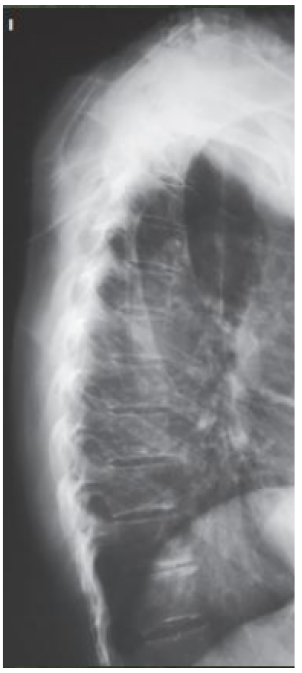
\includegraphics[width=0.3\linewidth]{imagenes/col79}
	 	\caption{Primer disparo}
	 	\label{fig:col79}
	 \end{figure}
	 
	 % TODO: \usepackage{graphicx} required
	 \begin{figure}
	 	\centering
	 	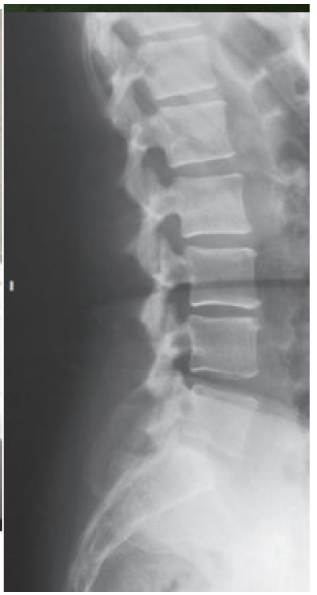
\includegraphics[width=0.3\linewidth]{imagenes/col81}
	 	\caption{Segundo disparo}
	 	\label{fig:col81}
	 \end{figure}
	 
	 
	 \twocolumn
	 \clearpage
	
	%----------------------------------------------------------
	%  Para agregar otro enfoque duplicá el bloque
	%  desde \subsection hasta \textbf{Trucos}
	%----------------------------------------------------------
	% \input{secciones/craneo}
	
\end{document}